%\documentclass[table]{article}
%\usepackage{beamerarticle}
\documentclass[10pt,xcolor=table,ignorenonframetext,handout,aspectratio=169]{beamer}
%\documentclass[10pt,xcolor=table,ignorenonframetext]{beamer}
\mode<presentation>
{
  \usetheme{default}
  \useoutertheme{split}
% \usefonttheme{serif}
}

\usenavigationsymbolstemplate{}
\usepackage{amssymb}
\usepackage{amsmath}
\usepackage{setspace}
\usepackage{graphicx}
\usepackage{multirow}
\usepackage[english]{babel}
\usepackage[latin1]{inputenc}
\usepackage{bm}
\usepackage{graphicx}
\usepackage{multirow}
\usepackage{tikz}
\usepackage[english]{babel}
\usepackage[latin1]{inputenc}
%\usepackage{ulem}
\usepackage{pifont}
\usepackage{changepage}
%\usepackage{colortbl}
%\usepackage[table]{xcolor}
%\usepackage{xcolor}

\setbeamersize{text margin left=1cm,text margin right=5cm}

\setbeamertemplate{itemize item}[circle]
\setbeamertemplate{frametitle}[default][center]

\newlength{\wideitemsep}
\setlength{\wideitemsep}{\itemsep}
\addtolength{\wideitemsep}{4pt}
\let\olditem\item
\renewcommand{\item}{\setlength{\itemsep}{\wideitemsep}\olditem}

\newcommand{\HRule}{\rule{0.5\textwidth}{0.05mm}}

\usetikzlibrary{arrows,positioning,shapes}
\usetikzlibrary{decorations.pathreplacing}
\usetikzlibrary{snakes}

\definecolor{blueish}{RGB}{97,156,255}
\definecolor{greenish}{RGB}{0,186,56}
\definecolor{reddish}{RGB}{248,118,109}

\definecolor{oiverm}{RGB}{213,94,0}
\definecolor{oiblue}{RGB}{0,114,178}
\definecolor{oigreen}{RGB}{0,158,115}
\definecolor{oipurple}{RGB}{204,121,167}
\definecolor{oiorange}{RGB}{230,159,0}
\definecolor{oisky}{RGB}{86,180,233}
\definecolor{oiyellow}{RGB}{240,228,66}
\definecolor{williams}{RGB}{81,38,152}

\definecolor{hue1}{RGB}{255,255,204}
\definecolor{hue2}{RGB}{161,218,180}
\definecolor{hue3}{RGB}{65,182,196}
\definecolor{hue4}{RGB}{44,127,184}
\definecolor{hue5}{RGB}{37,52,148}

\definecolor{dvg1}{RGB}{213,62,79}
\definecolor{dvg2}{RGB}{244,109,67}
\definecolor{dvg3}{RGB}{253,174,97}
\definecolor{dvg4}{RGB}{254,224,139}
\definecolor{dvg5}{RGB}{230,245,152}
\definecolor{dvg6}{RGB}{171,221,164}
\definecolor{dvg7}{RGB}{102,194,165}
\definecolor{dvg8}{RGB}{50,136,189}

\setbeamercolor{structure}{fg=williams,bg=williams!12}

\title{False Counterfactuals, Slide \insertframenumber}
\subtitle{}

\author{Economics 379 (Professor Jakiela)}
\date{}



\begin{document}
	
	
	
%%%%%%%%%%%%%%%%%%%%%%%%%%%%%%%%%%%%%%%%%%%%%%%%%%%%%%%%%%%%%%%%%%%%%%%%%%
	% COURSE Title slide
%%%%%%%%%%%%%%%%%%%%%%%%%%%%%%%%%%%%%%%%%%%%%%%%%%%%%%%%%%%%%%%%%%%%%%%%%%
	
\begin{frame}<beamer:0>[plain]
	
	\begin{center}
		\begin{tikzpicture}
		
		\node [opacity=1] (bg)  {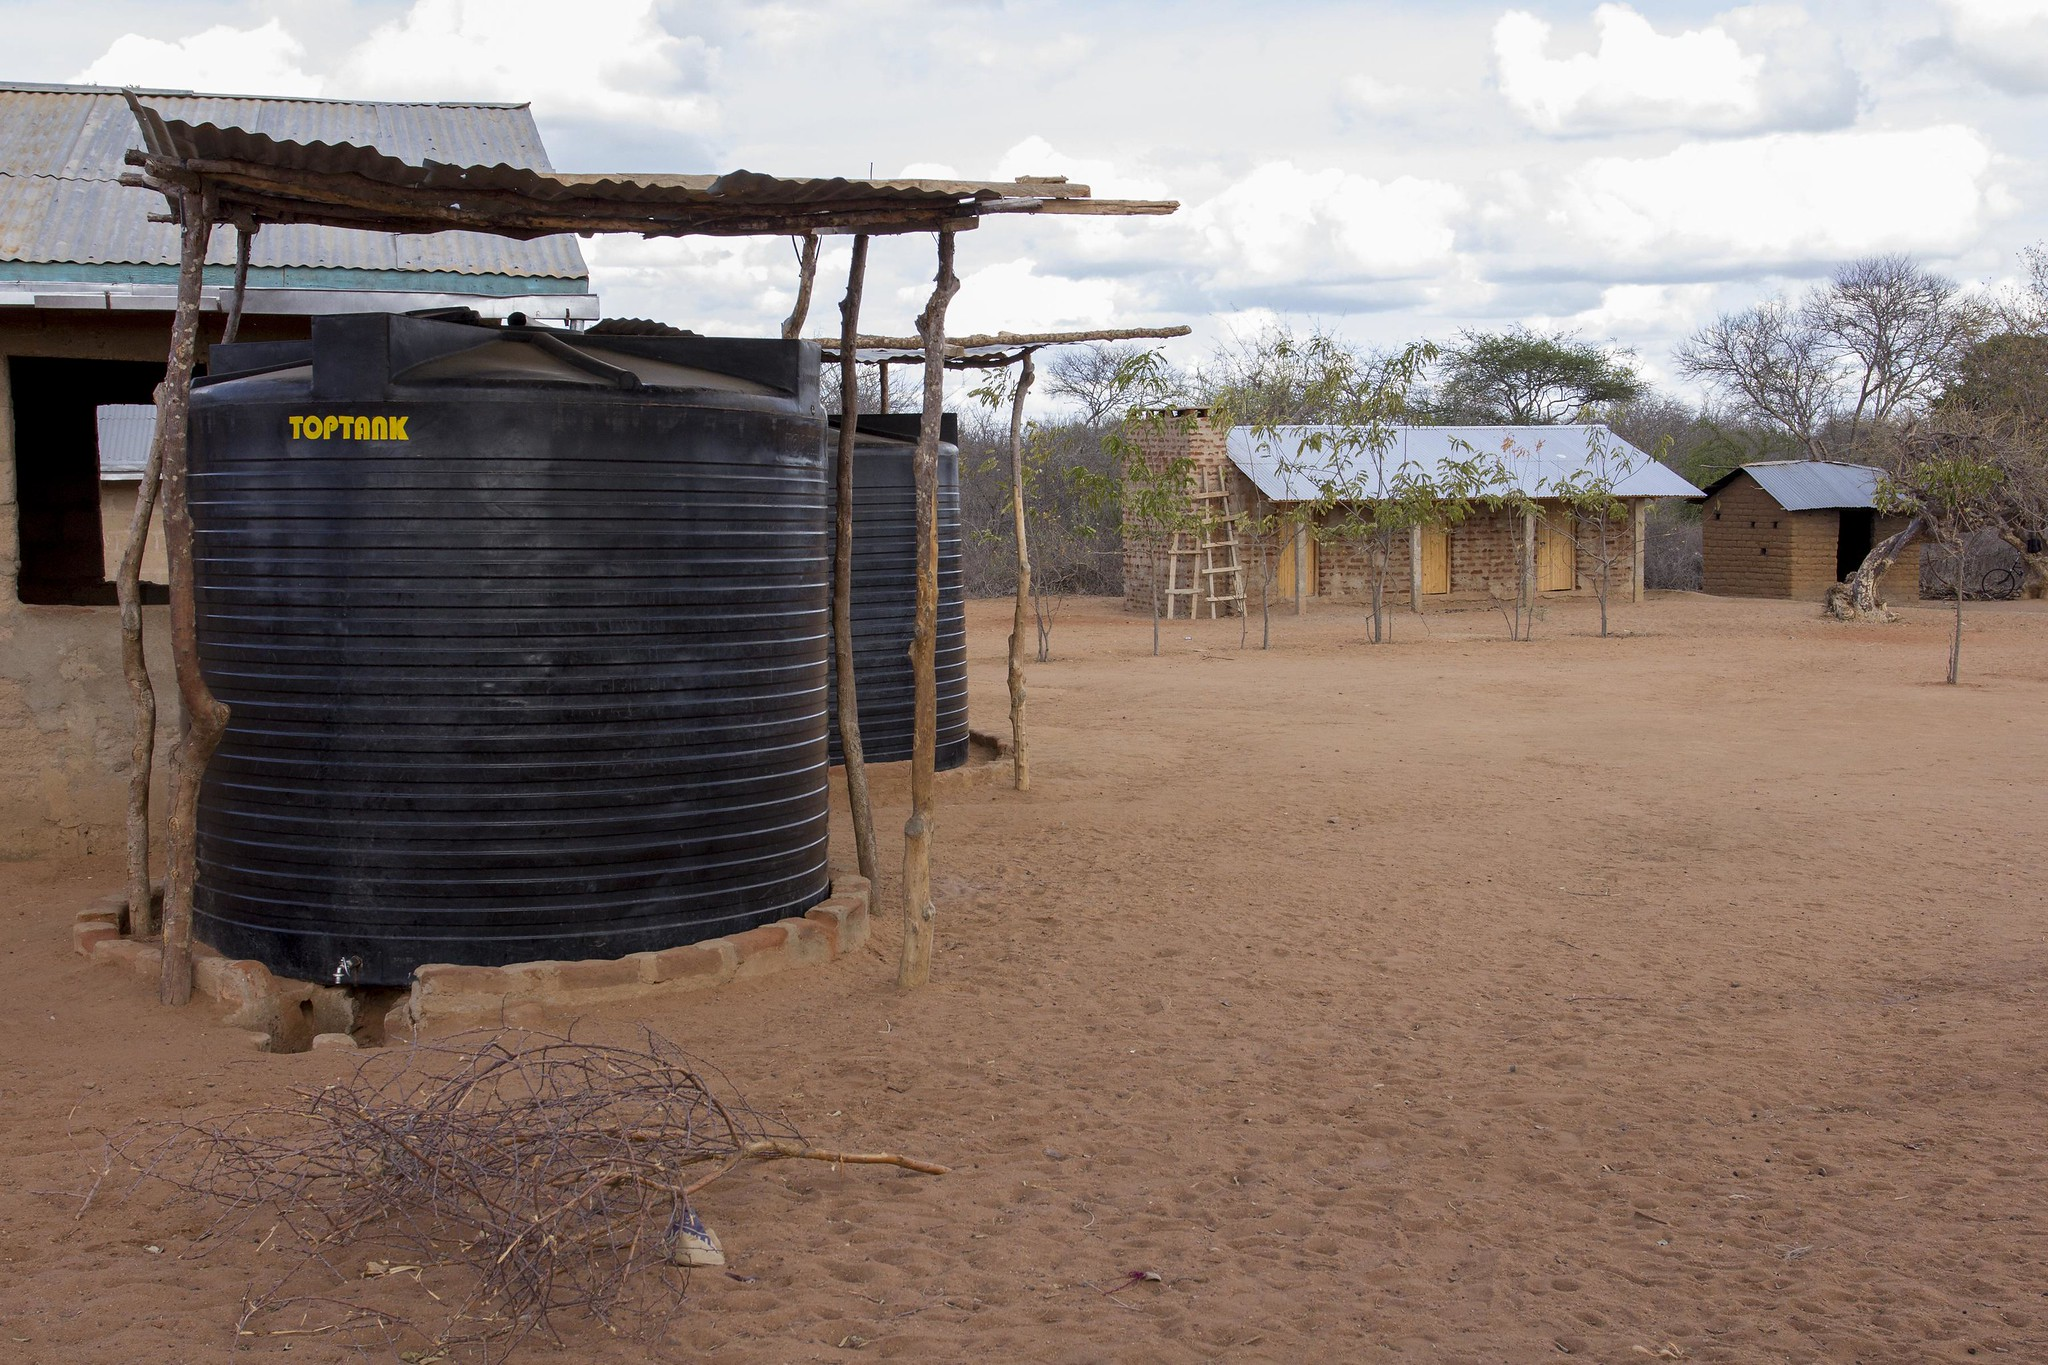
\includegraphics[keepaspectratio,height=0.9\paperheight]{photos/Kenya-cistern-Flore-de-Preneuf-2011-LARGE.jpg}};
		
		\node [anchor=east,align=right] at (6,-2.25) {\Large{\textcolor{white}{Williams College ECON 379:}}};		
		\node [anchor=east,align=right] at (6,-3) {\Large{\textcolor{white}{Program Evaluation for International Development}}};

		\node [anchor=east] at (6,-3.8) {\textcolor{yellow}{\tiny{photo:  Flore de Preneuf / World Bank}}};
		
		\end{tikzpicture}
	\end{center}
\end{frame}


%%%%%%%%%%%%%%%%%%%%%%%%%%%%%%%%%%%%%%%%%%%%%%%%%%%%%%%%%%%%%%%%%%%%%%%%%%
% LECTURE Title slide
%%%%%%%%%%%%%%%%%%%%%%%%%%%%%%%%%%%%%%%%%%%%%%%%%%%%%%%%%%%%%%%%%%%%%%%%%%

\begin{frame}[plain]

\only<beamer>{\begin{adjustwidth}{0cm}{-4cm}}

\begin{center}
	\begin{tikzpicture}
	
	\node [opacity=0.25] (bg)  {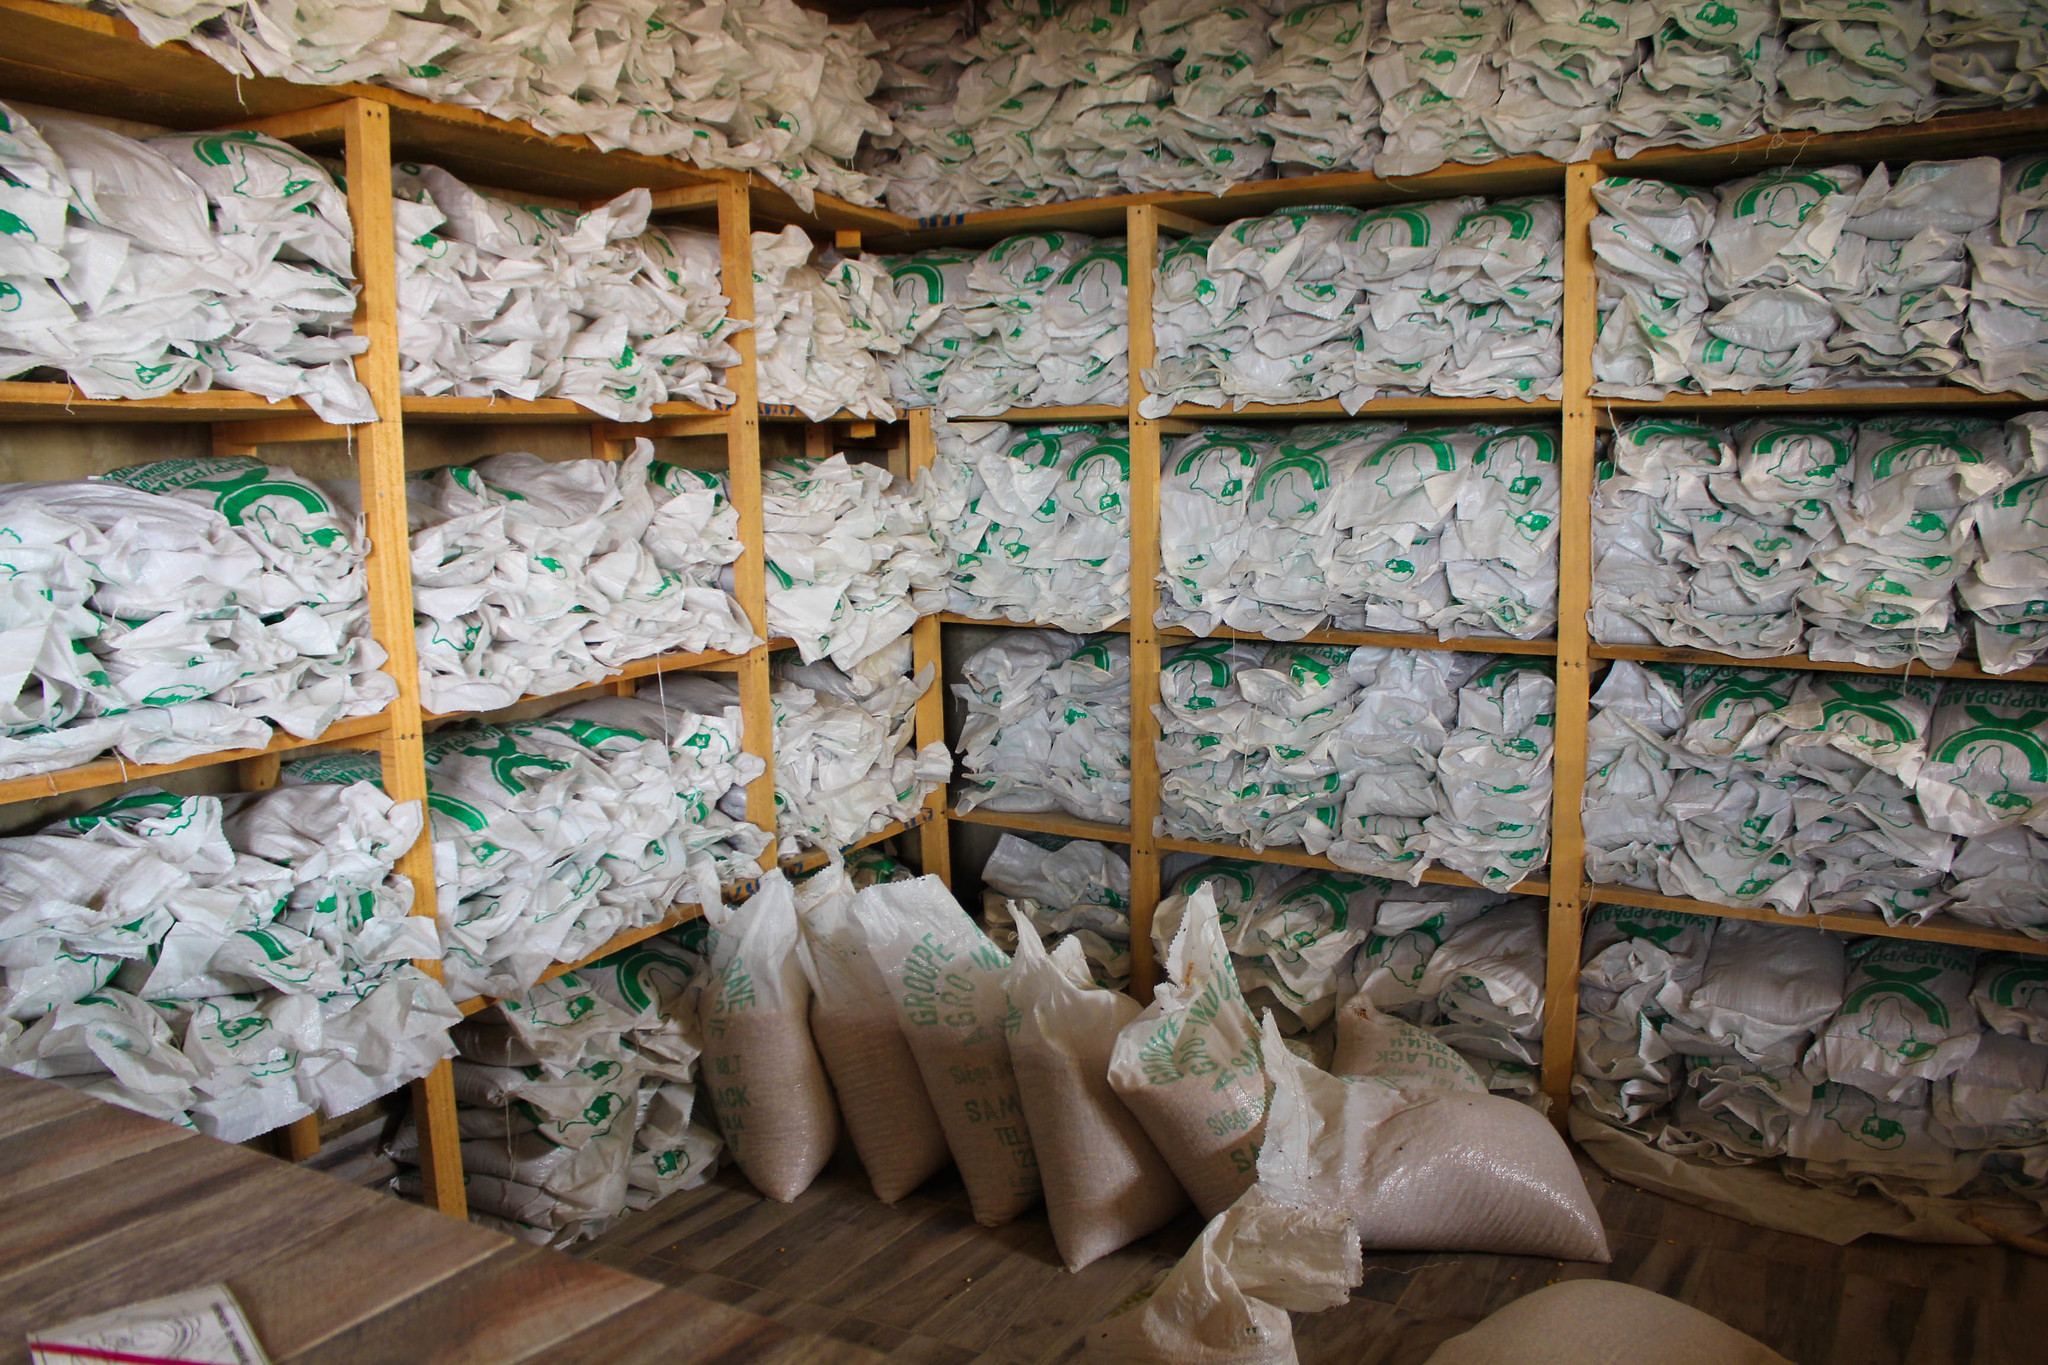
\includegraphics[keepaspectratio,height=0.9\paperheight]{photos/Senegal-WAAPP-seeds-Daniella-Van-Leggelo-Padilla-LARGE.jpg}};
	
	\node at (0,2.5) {\large{\textcolor{williams}{Williams College ECON 379:}}};		
	\node at (0,1.5) {\large{\textcolor{williams}{Program Evaluation for International Development}}};
	
	\node at (0,-0.5) {\large{\textcolor{williams}{\textbf{Module 3: False Counterfactuals}}}};
	
	\node at (0,-2) {\large{\textcolor{williams}{Professor:  Pamela Jakiela}}};
	
	\node [anchor=east] at (6,-3.8) {\textcolor{yellow}{\tiny{photo:  Daniella Van Leggelo-Padilla / World Bank}}};
	
	\end{tikzpicture}
\end{center}
\only<beamer>{\end{adjustwidth}}
\end{frame}


%%%%%%%%%%%%%%%%%%%%%%%%%%%%%%%%%%%%%%%%%%%%%%%%%%%%%%%%%%%%%%%%%%%%%%%%%%%

\begin{frame}[plain]

\only<beamer>{\begin{adjustwidth}{0cm}{-4cm}}
	
	\begin{center}
		
		\Large{\textcolor{williams}{False Counterfactuals}}
		
	\end{center}
	
	\only<beamer>{\end{adjustwidth}}
\end{frame}


%%%%%%%%%%%%%%%%%%%%%%%%%%%%%%%%%%%%%%%%%%%%%%%%%%%%%%%%%%%%%%%%%%%%%

\begin{frame}{False Counterfactual \#1}

\medskip
\textbf{Participant vs.~Non-Participant Comparisons:}

\medskip
\begin{itemize}
	
	\item
	Compares individuals/communities/units/etc that chose \\
	to participate in a program to those that did not
	
	\item 
	Treatment effect conflated with \ldots ?
	
\end{itemize}

\pause
\medskip
\medskip
\textbf{The Experimental Ideal:}

\medskip
\begin{itemize}
	
	\item
	Treatment is randomly assigned
	
	\item
	Treatment, control groups similar in terms of observable, unobservable characteristics (at least in expectation)
	
	\item 
	Difference in means $=$ unbiased estimate of treatment effect
	
\end{itemize}

\end{frame}



%%%%%%%%%%%%%%%%%%%%%%%%%%%%%%%%%%%%%%%%%%%%%%%%%%%%%%%%%%%%%%%%%%%%%%%

\begin{frame}{False Counterfactual \#2:  Before/After Comparison}

\begin{center}
	\begin{tikzpicture}
	
	% blank canvas
	\only<handout>{\fill[fill=white,draw=white,ultra thin]
		(0,0) -- (11,0) -- (11,6) -- (0,6) -- cycle;}
	\only<beamer>{\fill[fill=white,draw=white,ultra thin]
		(0,0) -- (14,0) -- (14,6) -- (0,6) -- cycle;}
	\only<beamer>{\draw[draw=oiblue!60,fill=oiblue!10,opacity=0.5] (11,1) rectangle (14,5);}
	%\draw[step=1.0,gray!20,thin] (0,0) grid (11,6);
	
	%	\pgfmathsetmacro\xshift{0.5cm};
	%	\pgfmathsetmacro\yshift{5.5cm};
	
	\pgfmathsetmacro\mycolor{"oiblue!72"};
	
	\filldraw [\mycolor] (1,2.95) -- (1,3.05) -- (8,3.05) -- (8,2.95) -- cycle;
	\filldraw [\mycolor] (8,2.75) -- (8,3.25) -- (8.5,3) -- cycle;
	
	\node [oiverm,anchor=south,align=center] at (4.5,3.25) {\textbf{treatment}};
	\draw [oiverm, thick] (4.5,3.25) -- (4.5,2.75) ;
	
	\node [oigreen,anchor=north,align=center,text width = 3.2 cm] at (6,2.75) {post-treatment \\
		outcomes: \\
	$Y_{post,i}$};
	\draw [oigreen, thick] (6,3.25) -- (6,2.75) ;

	
	\node [oigreen,anchor=north,align=center,text width = 3.2 cm] at (3,2.75) {pre-treatment \\
		outcomes: \\
		$Y_{pre,i}$};
	\draw [oigreen, thick] (3,3.25) -- (3,2.75) ;
		
	\end{tikzpicture}
\end{center}
\end{frame}



%%%%%%%%%%%%%%%%%%%%%%%%%%%%%%%%%%%%%%%%%%%%%%%%%%%%%%%%%%%%%%%%%%%%%%%

\begin{frame}<handout:0>{False Counterfactual \#2:  Before/After Comparison}

\begin{center}
	\begin{tikzpicture}
	
	% blank canvas
	\only<handout>{\fill[fill=white,draw=white,ultra thin]
		(0,0) -- (11,0) -- (11,6) -- (0,6) -- cycle;}
	\only<beamer>{\fill[fill=white,draw=white,ultra thin]
		(0,0) -- (14,0) -- (14,6) -- (0,6) -- cycle;}
	\only<beamer>{\draw[draw=oiblue!60,fill=oiblue!10,opacity=0.5] (11,1) rectangle (14,5);}
	%\draw[step=1.0,gray!20,thin] (0,0) grid (11,6);
	
	%	\pgfmathsetmacro\xshift{0.5cm};
	%	\pgfmathsetmacro\yshift{5.5cm};
	
	\pgfmathsetmacro\mycolor{"oiblue!72"};
	
	\filldraw [\mycolor] (1,2.95) -- (1,3.05) -- (8,3.05) -- (8,2.95) -- cycle;
	\filldraw [\mycolor] (8,2.75) -- (8,3.25) -- (8.5,3) -- cycle;
	
	\node [oiverm,anchor=south,align=center] at (4.5,3.25) {\textbf{treatment}};
	\draw [oiverm, thick] (4.5,3.25) -- (4.5,2.75) ;
	
	\node [gray,anchor=south,align=center] at (4.5,4.5) {what else happened?};
	\draw [gray, ->] (3.325,4.5) -- (3.325,3.325) ;
	\draw [gray, ->] (5.625,4.5) -- (5.625,3.25) ;
	
	\node [oigreen,anchor=north,align=center,text width = 3.2 cm] at (6,2.75) {post-treatment \\
		outcomes: \\
		$Y_{post,i}$};
	\draw [oigreen, thick] (6,3.25) -- (6,2.75) ;
	
	
	\node [oigreen,anchor=north,align=center,text width = 3.2 cm] at (3,2.75) {pre-treatment \\
		outcomes: \\
		$Y_{pre,i}$};
	\draw [oigreen, thick] (3,3.25) -- (3,2.75) ;
	
	\end{tikzpicture}
\end{center}
\end{frame}



%%%%%%%%%%%%%%%%%%%%%%%%%%%%%%%%%%%%%%%%%%%%%%%%%%%%%%%%%%%%%%%%%%%%%

\begin{frame}{Three Approaches to Estimating Treatment Effects}

\medskip
Any of these \textbf{can} be credible (all require assumptions):

\medskip
\begin{enumerate}
	
	\item
	The experimental ideal:  randomized treatment vs.~control
	
	\item
	Participant vs.~non-participant comparisons $\rightarrow$ selection bias?
	
	\item 
	Pre vs.~post comparisons $\rightarrow$ changes over time?
	
\end{enumerate}

\medskip
\medskip
In each case, we ask:

\medskip
\begin{enumerate}
	
	\item
	Is there a difference (in means) between groups?
	
	\item
	Is that difference likely to have occurred by chance?
	
	\item 
	Should we interpret difference as causal effect of treatment?
	
\end{enumerate}

\end{frame}



%%%%%%%%%%%%%%%%%%%%%%%%%%%%%%%%%%%%%%%%%%%%%%%%%%%%%%%%%%%%%%%%%%%%%%%

\begin{frame}<handout:0>{Testing $H_0: \bar{Y}_T =\bar{Y}_C$ }

\begin{center}
	\begin{tikzpicture}
	
	% blank canvas
	\only<handout>{\fill[fill=white,draw=white,ultra thin]
		(0,0) -- (11,0) -- (11,6) -- (0,6) -- cycle;}
	\only<beamer>{\fill[fill=white,draw=white,ultra thin]
		(0,0) -- (14,0) -- (14,6) -- (0,6) -- cycle;}
	\only<beamer>{\draw[draw=oiblue!60,fill=oiblue!10,opacity=0.5] (11,1) rectangle (14,5);}
	%\draw[step=1.0,gray!20,thin] (0,0) grid (11,6);
	
	%\pgfmathsetmacro\mycolor{"oiblue!72"};
	
	\node [anchor=north,opacity=1] at (2.5,6)  {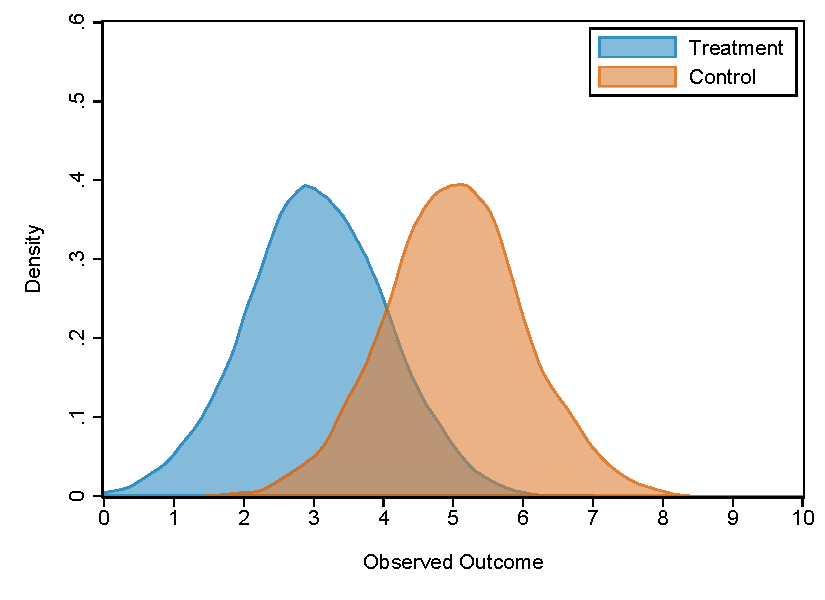
\includegraphics[keepaspectratio,width=4.8cm]{fig/TvsC-density.pdf}};

	\pgfmathsetmacro\xshift{5cm};
	\pgfmathsetmacro\yshift{5.75cm};	
	\node [anchor=north west,align=left,text width = 5.5cm,xshift=\xshift,yshift=\yshift] (text1) at (0,0) {\small{When $\bar{Y}_T$ and $\bar{Y}_C$ are independent:}};
	%\node [anchor=north west,align=left,text width = 5.5cm,] (text2) at (text1.south west) {\small{$SE \left(\bar{Y}_T - \bar{Y}_C \right) = \sqrt{\textcolor{red}{s^2_T / n_T} + \textcolor{red}{s^2_C / n_C}}$}};
	\node [anchor=north west,align=left,text width = 5.5cm,] (text2) at (text1.south west) {\small{$SE \left(\bar{Y}_T - \bar{Y}_C \right) = \sqrt{\textcolor{black}{SE^2_{\bar{Y}_T}} + \textcolor{black}{SE^2_{\bar{Y}_C}}}$}};
	
	\end{tikzpicture}
\end{center}
\end{frame}


%%%%%%%%%%%%%%%%%%%%%%%%%%%%%%%%%%%%%%%%%%%%%%%%%%%%%%%%%%%%%%%%%%%%%%%

\begin{frame}{Testing $H_0: \bar{Y}_T =\bar{Y}_C$ }

\begin{center}
	\begin{tikzpicture}
	
	% blank canvas
	\only<handout>{\fill[fill=white,draw=white,ultra thin]
		(0,0) -- (11,0) -- (11,6) -- (0,6) -- cycle;}
	\only<beamer>{\fill[fill=white,draw=white,ultra thin]
		(0,0) -- (14,0) -- (14,6) -- (0,6) -- cycle;}
	\only<beamer>{\draw[draw=oiblue!60,fill=oiblue!10,opacity=0.5] (11,1) rectangle (14,5);}
	%\draw[step=1.0,gray!20,thin] (0,0) grid (11,6);
	
	%\pgfmathsetmacro\mycolor{"oiblue!72"};
	
	\node [anchor=north,opacity=1] at (2.5,6)  {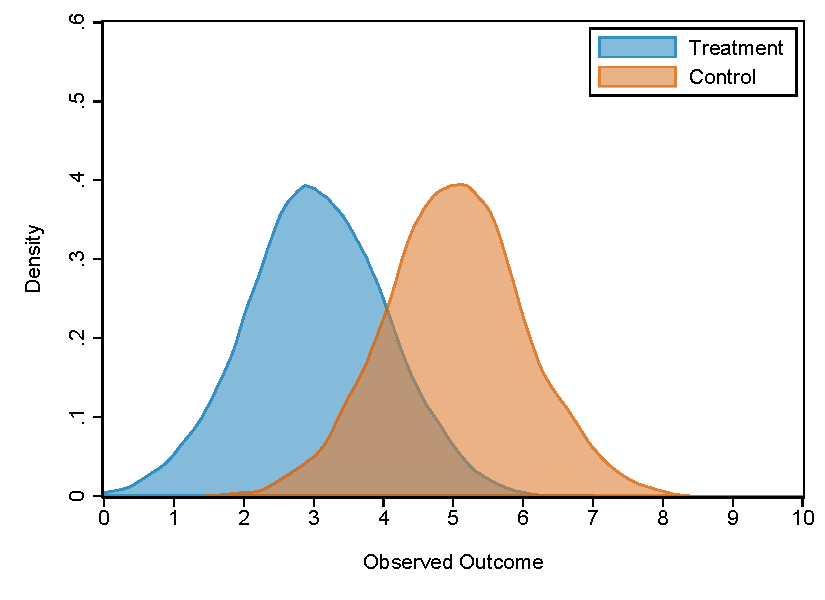
\includegraphics[keepaspectratio,width=4.8cm]{fig/TvsC-density.pdf}};
	
	\pgfmathsetmacro\xshift{5cm};
	\pgfmathsetmacro\yshift{5.75cm};	
	\node [anchor=north west,align=left,text width = 5.5cm,xshift=\xshift,yshift=\yshift] (text1) at (0,0) {\small{When $\bar{Y}_T$ and $\bar{Y}_C$ are independent:}};
	%\node [anchor=north west,align=left,text width = 5.5cm,] (text2) at (text1.south west) {\small{$SE \left(\bar{Y}_T - \bar{Y}_C \right) = \sqrt{\textcolor{red}{s^2_T / n_T} + \textcolor{red}{s^2_C / n_C}}$}};
	\node [anchor=north west,align=left,text width = 5.5cm,] (text2) at (text1.south west) {\small{$SE \left(\bar{Y}_T - \bar{Y}_C \right) = \sqrt{\textcolor{red}{SE^2_{\bar{Y}_T}} + \textcolor{black}{SE^2_{\bar{Y}_C}}}$}};
	
	\node [anchor=north,align=center] (lbl1) at ([xshift=0.2cm,yshift=-0.5cm]text2.south) {\small{$\textcolor{red}{=}$}};
	\draw[red,->] (lbl1.north) -- ([yshift=0.625cm]lbl1.north);
	\node [anchor=east,align=right] (lbl1A) at (lbl1.west) {\small{$\textcolor{red}{SE_{\bar{Y}_T}}$}};
	\node [anchor=west,align=left] (lbl1C) at (lbl1.east) {\small{$\textcolor{red}{\sqrt{\frac{s^2_T}{n_T}}}$}};
	\node [anchor=north,align=center] (lbl2) at ([yshift=-0.5cm]lbl1.south) {\small{$\textcolor{red}{=}$}};
	\node [anchor=west,align=left] (lbl2C) at (lbl2.east) {\small{$\textcolor{red}{\sqrt{\frac{ \sum_{i \in T} \left( Y_i - \bar{Y} \right)^2 }{ n_T \left( n_T - 1 \right)  }}}$}};
	\node [red,anchor=north,align=center,text width=5cm] (lbl3) at ([yshift=-0.5cm]lbl2.south) {\small{where $n_T$ is treatment observations, and $\sum_{i \in T}$ sums over treated $i$}};
	
	\end{tikzpicture}
\end{center}
\end{frame}



%%%%%%%%%%%%%%%%%%%%%%%%%%%%%%%%%%%%%%%%%%%%%%%%%%%%%%%%%%%%%%%%%%%%%%%

\begin{frame}<handout:0>{Testing $H_0: \bar{Y}_T =\bar{Y}_C$ }

\begin{center}
	\begin{tikzpicture}
	
	% blank canvas
	\only<handout>{\fill[fill=white,draw=white,ultra thin]
		(0,0) -- (11,0) -- (11,6) -- (0,6) -- cycle;}
	\only<beamer>{\fill[fill=white,draw=white,ultra thin]
		(0,0) -- (14,0) -- (14,6) -- (0,6) -- cycle;}
	\only<beamer>{\draw[draw=oiblue!60,fill=oiblue!10,opacity=0.5] (11,1) rectangle (14,5);}
	%\draw[step=1.0,gray!20,thin] (0,0) grid (11,6);
	
	%\pgfmathsetmacro\mycolor{"oiblue!72"};
	
	\node [anchor=north,opacity=1] at (2.5,6)  {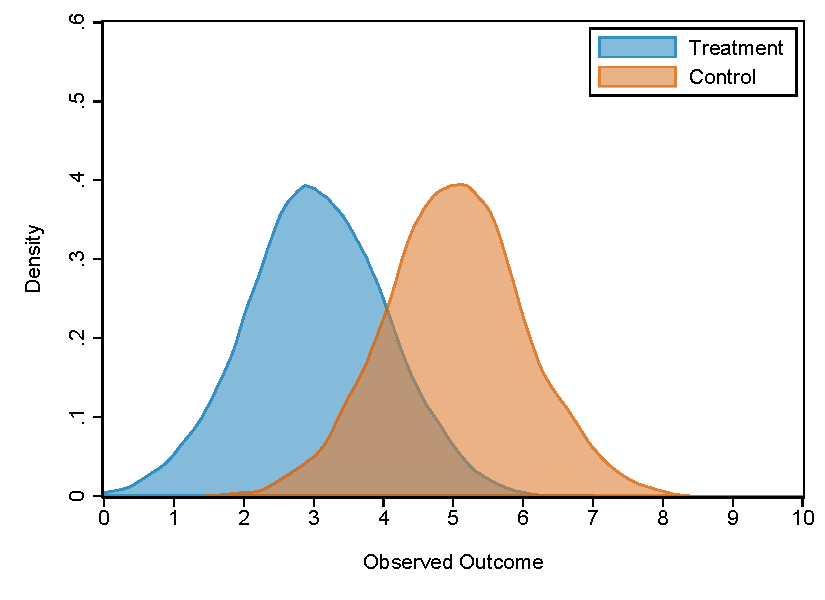
\includegraphics[keepaspectratio,width=4.8cm]{fig/TvsC-density.pdf}};
	
	\pgfmathsetmacro\xshift{5cm};
	\pgfmathsetmacro\yshift{5.75cm};	
	\node [anchor=north west,align=left,text width = 5.5cm,xshift=\xshift,yshift=\yshift] (text1) at (0,0) {\small{When $\bar{Y}_T$ and $\bar{Y}_C$ are independent:}};
	\node [anchor=north west,align=left,text width = 5.5cm,] (text2) at (text1.south west) {\small{$SE \left(\bar{Y}_T - \bar{Y}_C \right) = \sqrt{\textcolor{black}{SE^2_{\bar{Y}_T}} + \textcolor{black}{SE^2_{\bar{Y}_C}}}$}};

	%\node [anchor=north west,align=left,text width = 5.5cm,] (text3) at ([yshift=-0.5cm]text2.south west) {\small{$\Rightarrow t = \frac{\bar{Y}_T - \bar{Y}_C}{\sqrt{SE^2_{\bar{Y}_T} + SE^2_{\bar{Y}_C}}}$}};	
	\node [red,anchor=north west,align=left,text width = 5.5cm,] (text3) at ([yshift=-0.25cm]text2.south west) {\small{$\Rightarrow t = \left( \bar{Y}_T - \bar{Y}_C \right) / \sqrt{SE^2_{\bar{Y}_T} + SE^2_{\bar{Y}_C}}$}};
		
%	\node [anchor=north west,align=left,text width = 5.5cm,] (text4) at ([yshift=-0.25cm]text3.south west) {\small{$\Rightarrow $ p-value -- which is what, again?}};	
%	
%	\node [gray,anchor=north,align=center,text width = 5.5cm,] (text5) at (text4.south) {\footnotesize{probability of a t-stat that big \\
%			occurring under the null}};	

	\end{tikzpicture}
\end{center}
\end{frame}



%%%%%%%%%%%%%%%%%%%%%%%%%%%%%%%%%%%%%%%%%%%%%%%%%%%%%%%%%%%%%%%%%%%%%%%

\begin{frame}<handout:0>{Testing $H_0: \bar{Y}_T =\bar{Y}_C$ }

\begin{center}
	\begin{tikzpicture}
	
	% blank canvas
	\only<handout>{\fill[fill=white,draw=white,ultra thin]
		(0,0) -- (11,0) -- (11,6) -- (0,6) -- cycle;}
	\only<beamer>{\fill[fill=white,draw=white,ultra thin]
		(0,0) -- (14,0) -- (14,6) -- (0,6) -- cycle;}
	\only<beamer>{\draw[draw=oiblue!60,fill=oiblue!10,opacity=0.5] (11,1) rectangle (14,5);}
	%\draw[step=1.0,gray!20,thin] (0,0) grid (11,6);
	
	%\pgfmathsetmacro\mycolor{"oiblue!72"};
	
	\node [anchor=north,opacity=1] at (2.5,6)  {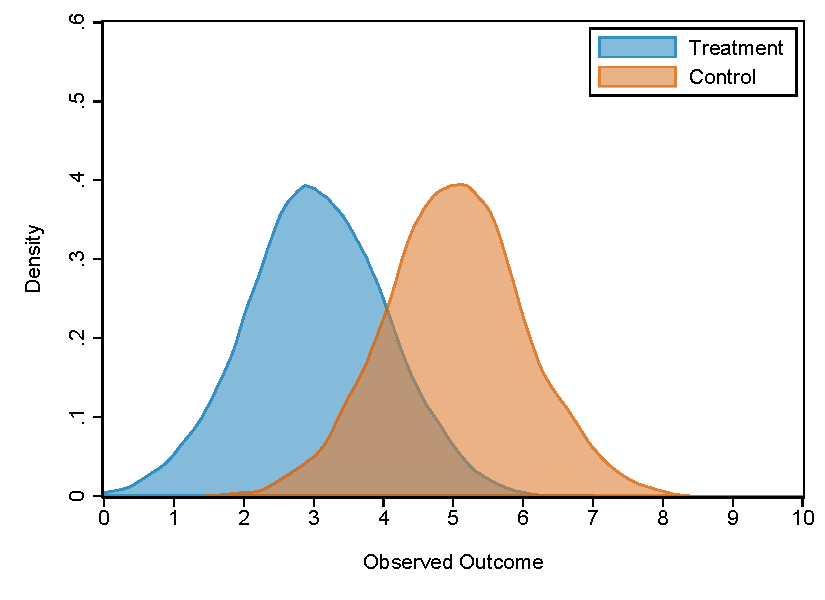
\includegraphics[keepaspectratio,width=4.8cm]{fig/TvsC-density.pdf}};
	
	\pgfmathsetmacro\xshift{5cm};
	\pgfmathsetmacro\yshift{5.75cm};	
	\node [anchor=north west,align=left,text width = 5.5cm,xshift=\xshift,yshift=\yshift] (text1) at (0,0) {\small{When $\bar{Y}_T$ and $\bar{Y}_C$ are independent:}};
	\node [anchor=north west,align=left,text width = 5.5cm,] (text2) at (text1.south west) {\small{$SE \left(\bar{Y}_T - \bar{Y}_C \right) = \sqrt{\textcolor{black}{SE^2_{\bar{Y}_T}} + \textcolor{black}{SE^2_{\bar{Y}_C}}}$}};
	
	%\node [anchor=north west,align=left,text width = 5.5cm,] (text3) at ([yshift=-0.5cm]text2.south west) {\small{$\Rightarrow t = \frac{\bar{Y}_T - \bar{Y}_C}{\sqrt{SE^2_{\bar{Y}_T} + SE^2_{\bar{Y}_C}}}$}};	
	\node [red,anchor=north west,align=left,text width = 5.5cm,] (text3) at ([yshift=-0.25cm]text2.south west) {\small{$\Rightarrow t = \left( \bar{Y}_T - \bar{Y}_C \right) / \sqrt{SE^2_{\bar{Y}_T} + SE^2_{\bar{Y}_C}}$}};
	
	\node [anchor=north west,align=left,text width = 5.5cm,] (text4) at ([yshift=-0.25cm]text3.south west) {\small{$\Rightarrow $ p-value -- which is what, again?}};	
	
	\node [gray,anchor=north,align=center,text width = 5.5cm,] (text5) at (text4.south) {\footnotesize{probability of a t-stat that big \\
			occurring under the null}};	
	
	\end{tikzpicture}
\end{center}
\end{frame}



%%%%%%%%%%%%%%%%%%%%%%%%%%%%%%%%%%%%%%%%%%%%%%%%%%%%%%%%%%%%%%%%%%%%%%%

\begin{frame}{Testing $H_0: \bar{Y}_T =\bar{Y}_C$ }

\begin{center}
	\begin{tikzpicture}
	
	% blank canvas
	\only<handout>{\fill[fill=white,draw=white,ultra thin]
		(0,0) -- (11,0) -- (11,6) -- (0,6) -- cycle;}
	\only<beamer>{\fill[fill=white,draw=white,ultra thin]
		(0,0) -- (14,0) -- (14,6) -- (0,6) -- cycle;}
	\only<beamer>{\draw[draw=oiblue!60,fill=oiblue!10,opacity=0.5] (11,1) rectangle (14,5);}
	%\draw[step=1.0,gray!20,thin] (0,0) grid (11,6);
	
	%\pgfmathsetmacro\mycolor{"oiblue!72"};
	
	\node [anchor=north,opacity=1] at (2.5,6)  {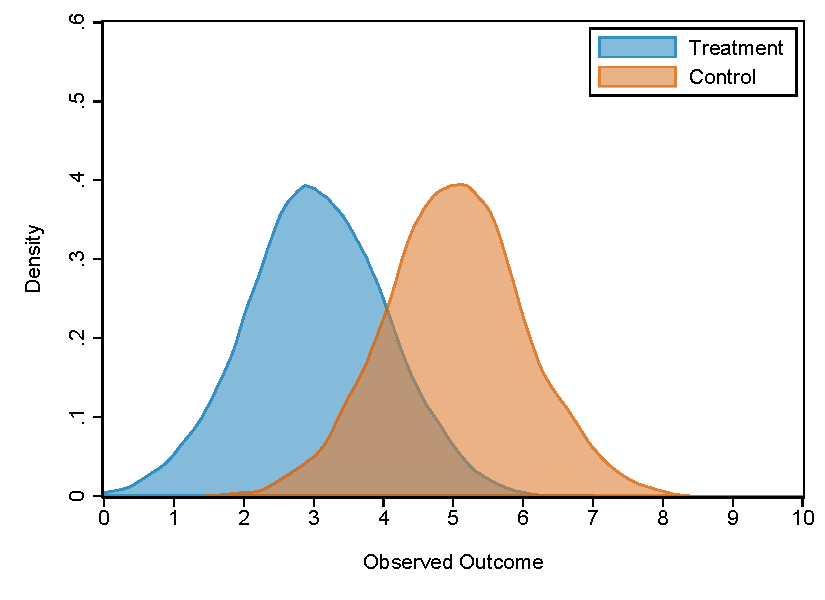
\includegraphics[keepaspectratio,width=4.8cm]{fig/TvsC-density.pdf}};
	
	\pgfmathsetmacro\xshift{5cm};
	\pgfmathsetmacro\yshift{5.75cm};	
	\node [anchor=north west,align=left,text width = 5.5cm,xshift=\xshift,yshift=\yshift] (text1) at (0,0) {\small{When $\bar{Y}_T$ and $\bar{Y}_C$ are independent:}};
	\node [anchor=north west,align=left,text width = 5.5cm,] (text2) at (text1.south west) {\small{$SE \left(\bar{Y}_T - \bar{Y}_C \right) = \sqrt{\textcolor{black}{SE^2_{\bar{Y}_T}} + \textcolor{black}{SE^2_{\bar{Y}_C}}}$}};
	
	%\node [anchor=north west,align=left,text width = 5.5cm,] (text3) at ([yshift=-0.5cm]text2.south west) {\small{$\Rightarrow t = \frac{\bar{Y}_T - \bar{Y}_C}{\sqrt{SE^2_{\bar{Y}_T} + SE^2_{\bar{Y}_C}}}$}};	
	\node [red,anchor=north west,align=left,text width = 5.5cm,] (text3) at ([yshift=-0.25cm]text2.south west) {\small{$\Rightarrow t = \left( \bar{Y}_T - \bar{Y}_C \right) / \sqrt{SE^2_{\bar{Y}_T} + SE^2_{\bar{Y}_C}}$}};
	
	\node [anchor=north west,align=left,text width = 5.5cm,] (text4) at ([yshift=-0.25cm]text3.south west) {\small{$\Rightarrow $ p-value -- which is what, again?}};	
	
	\node [anchor=north west,align=left,text width = 10.5cm,] at (0.25,2) {\small{When $\bar{Y}_T$ and $\bar{Y}_C$ are NOT independent, calculate the change, and \\ test null hypothesis that the mean (change in $Y$) is equal to 0}};	
	
	\end{tikzpicture}
\end{center}
\end{frame}


%%%%%%%%%%%%%%%%%%%%%%%%%%%%%%%%%%%%%%%%%%%%%%%%%%%%%%%%%%%%%%%%%%%%%%%

\begin{frame}<handout:0>{Testing $H_0: \bar{Y}_T =\bar{Y}_C$ in Stata}

\begin{center}
	\begin{tikzpicture}
	
	% blank canvas
	\only<handout>{\fill[fill=white,draw=white,ultra thin]
		(0,0) -- (11,0) -- (11,6) -- (0,6) -- cycle;}
	\only<beamer>{\fill[fill=white,draw=white,ultra thin]
		(0,0) -- (14,0) -- (14,6) -- (0,6) -- cycle;}
	\only<beamer>{\draw[draw=oiblue!60,fill=oiblue!10,opacity=0.5] (11,1) rectangle (14,5);}
	%\draw[step=1.0,gray!20,thin] (0,0) grid (11,6);
	
	%	\pgfmathsetmacro\xshift{3.5cm};
	%	\pgfmathsetmacro\yshift{5cm};	
	\node [anchor=north,opacity=1] at (3.5,5.5)  {\fbox{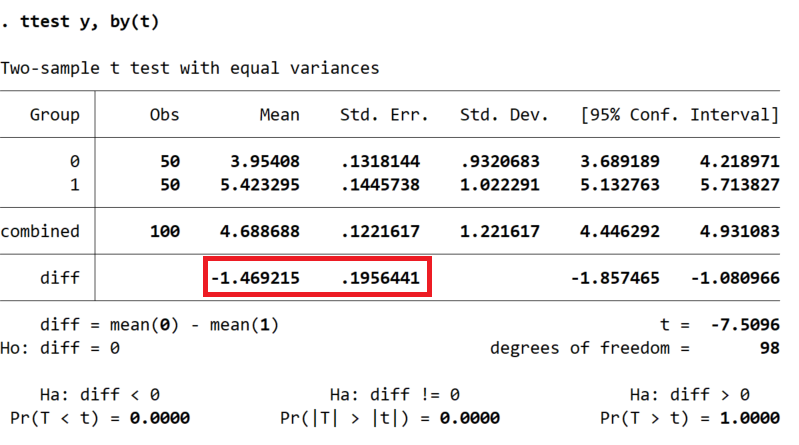
\includegraphics[keepaspectratio,width=6.4cm]{img/stata-ttest2A.png}}};
	
	%\node [red,anchor=north west,align=left,text width = 3.6cm] (text1) at (7,5) {\small{$\textcolor{red}{t } =  \frac{\bar{Y}_T - \bar{Y}_C}{SE \left( \bar{Y}_T - \bar{Y}_C \right) }$}};
	%\node [red,anchor=north west,align=left,text width = 3.6cm] (text2) at (text1.south west) {\small{$\textcolor{white}{t }  =  \frac{ - 1.4692 }{ 0.1956 }$}};
	%\node [red,anchor=north west,align=left,text width = 3.6cm] (text3) at (text2.south west) {\small{$\textcolor{white}{t }  = 7.5096$}};	
	%\draw[gray,thick,->] (3.875,3.125) -- (7,4.625);
	%\draw[red,thick,->] (7.25,3.3) -- (6.75,2.75);
	
	%\node [red,anchor=north west,align=left,text width = 10cm] (text4) at (0.1,1.25) {\small{To get p-value (in Stata): \texttt{display 2*(1 - abs(ttail(98,-7.5096)))}}};
	
	\end{tikzpicture}
\end{center}
\end{frame}


%%%%%%%%%%%%%%%%%%%%%%%%%%%%%%%%%%%%%%%%%%%%%%%%%%%%%%%%%%%%%%%%%%%%%%%

\begin{frame}<handout:0>{Testing $H_0: \bar{Y}_T =\bar{Y}_C$ in Stata}

\begin{center}
	\begin{tikzpicture}
	
	% blank canvas
	\only<handout>{\fill[fill=white,draw=white,ultra thin]
		(0,0) -- (11,0) -- (11,6) -- (0,6) -- cycle;}
	\only<beamer>{\fill[fill=white,draw=white,ultra thin]
		(0,0) -- (14,0) -- (14,6) -- (0,6) -- cycle;}
	\only<beamer>{\draw[draw=oiblue!60,fill=oiblue!10,opacity=0.5] (11,1) rectangle (14,5);}
	%\draw[step=1.0,gray!20,thin] (0,0) grid (11,6);
	
	%	\pgfmathsetmacro\xshift{3.5cm};
	%	\pgfmathsetmacro\yshift{5cm};	
	\node [anchor=north,opacity=1] at (3.5,5.5)  {\fbox{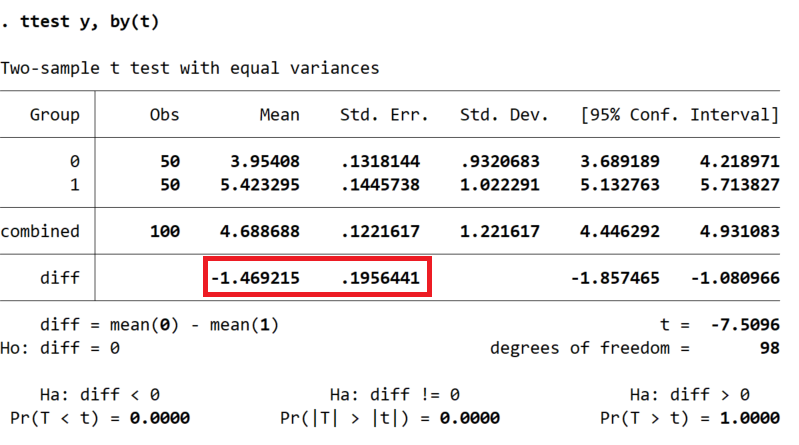
\includegraphics[keepaspectratio,width=6.4cm]{img/stata-ttest2A.png}}};
	
	\node [red,anchor=north west,align=left,text width = 3.6cm] (text1) at (7,5) {\small{$\textcolor{red}{t } =  \frac{\bar{Y}_T - \bar{Y}_C}{SE \left( \bar{Y}_T - \bar{Y}_C \right) }$}};
	%\node [red,anchor=north west,align=left,text width = 3.6cm] (text2) at (text1.south west) {\small{$\textcolor{white}{t }  =  \frac{ - 1.4692 }{ 0.1956 }$}};
	%\node [red,anchor=north west,align=left,text width = 3.6cm] (text3) at (text2.south west) {\small{$\textcolor{white}{t }  = 7.5096$}};	
	\draw[gray,thick,->] (3.875,3.125) -- (7,4.625);
	%\draw[red,thick,->] (7.25,3.3) -- (6.75,2.75);
	
	%\node [red,anchor=north west,align=left,text width = 10cm] (text4) at (0.1,1.25) {\small{To get p-value (in Stata): \texttt{display 2*(1 - abs(ttail(98,-7.5096)))}}};
	
	\end{tikzpicture}
\end{center}
\end{frame}


%%%%%%%%%%%%%%%%%%%%%%%%%%%%%%%%%%%%%%%%%%%%%%%%%%%%%%%%%%%%%%%%%%%%%%%

\begin{frame}<handout:0>{Testing $H_0: \bar{Y}_T =\bar{Y}_C$ in Stata}

\begin{center}
	\begin{tikzpicture}
	
	% blank canvas
	\only<handout>{\fill[fill=white,draw=white,ultra thin]
		(0,0) -- (11,0) -- (11,6) -- (0,6) -- cycle;}
	\only<beamer>{\fill[fill=white,draw=white,ultra thin]
		(0,0) -- (14,0) -- (14,6) -- (0,6) -- cycle;}
	\only<beamer>{\draw[draw=oiblue!60,fill=oiblue!10,opacity=0.5] (11,1) rectangle (14,5);}
	%\draw[step=1.0,gray!20,thin] (0,0) grid (11,6);
	
	%	\pgfmathsetmacro\xshift{3.5cm};
	%	\pgfmathsetmacro\yshift{5cm};	
	\node [anchor=north,opacity=1] at (3.5,5.5)  {\fbox{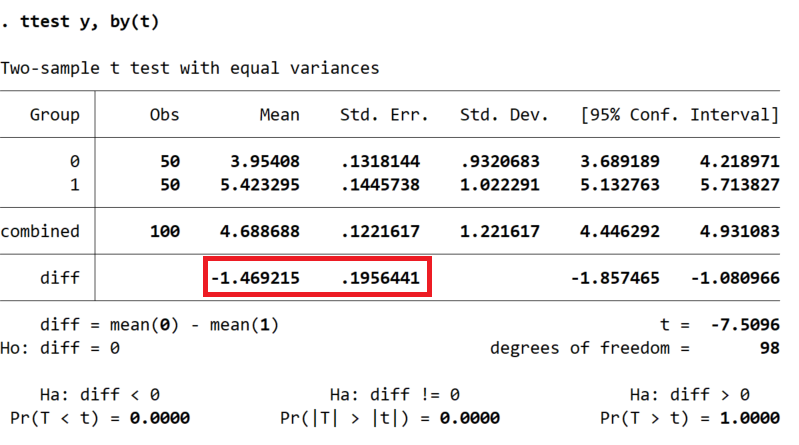
\includegraphics[keepaspectratio,width=6.4cm]{img/stata-ttest2A.png}}};
	
	\node [black,anchor=north west,align=left,text width = 3.6cm] (text1) at (7,5) {\small{$\textcolor{black}{t } =  \frac{\bar{Y}_T - \bar{Y}_C}{SE \left( \bar{Y}_T - \bar{Y}_C \right) }$}};
	\node [red,anchor=north west,align=left,text width = 3.6cm] (text2) at (text1.south west) {\small{$\textcolor{white}{t }  =  \frac{ - 1.4692 }{ 0.1956 }$}};
	%\node [red,anchor=north west,align=left,text width = 3.6cm] (text3) at (text2.south west) {\small{$\textcolor{white}{t }  = 7.5096$}};	
	\draw[gray,thick,->] (3.875,3.125) -- (7,4.625);
	%\draw[red,thick,->] (7.25,3.3) -- (6.75,2.75);
	
	%\node [red,anchor=north west,align=left,text width = 10cm] (text4) at (0.1,1.25) {\small{To get p-value (in Stata): \texttt{display 2*(1 - abs(ttail(98,-7.5096)))}}};
	
	\end{tikzpicture}
\end{center}
\end{frame}


%%%%%%%%%%%%%%%%%%%%%%%%%%%%%%%%%%%%%%%%%%%%%%%%%%%%%%%%%%%%%%%%%%%%%%%

\begin{frame}<handout:0>{Testing $H_0: \bar{Y}_T =\bar{Y}_C$ in Stata}

\begin{center}
	\begin{tikzpicture}
	
	% blank canvas
	\only<handout>{\fill[fill=white,draw=white,ultra thin]
		(0,0) -- (11,0) -- (11,6) -- (0,6) -- cycle;}
	\only<beamer>{\fill[fill=white,draw=white,ultra thin]
		(0,0) -- (14,0) -- (14,6) -- (0,6) -- cycle;}
	\only<beamer>{\draw[draw=oiblue!60,fill=oiblue!10,opacity=0.5] (11,1) rectangle (14,5);}
	%\draw[step=1.0,gray!20,thin] (0,0) grid (11,6);
	
	%	\pgfmathsetmacro\xshift{3.5cm};
	%	\pgfmathsetmacro\yshift{5cm};	
	\node [anchor=north,opacity=1] at (3.5,5.5)  {\fbox{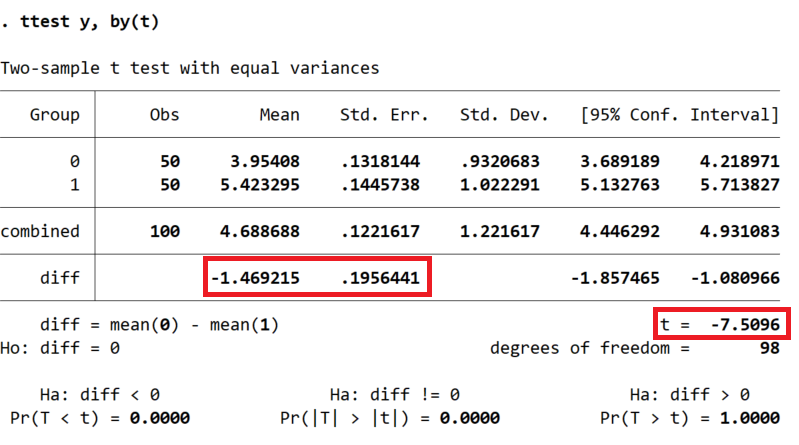
\includegraphics[keepaspectratio,width=6.4cm]{img/stata-ttest2B.png}}};
	
	\node [black,anchor=north west,align=left,text width = 3.6cm] (text1) at (7,5) {\small{$\textcolor{black}{t } =  \frac{\bar{Y}_T - \bar{Y}_C}{SE \left( \bar{Y}_T - \bar{Y}_C \right) }$}};
	\node [black,anchor=north west,align=left,text width = 3.6cm] (text2) at (text1.south west) {\small{$\textcolor{white}{t }  =  \frac{ - 1.4692 }{ 0.1956 }$}};
	\node [red,anchor=north west,align=left,text width = 3.6cm] (text3) at (text2.south west) {\small{$\textcolor{white}{t }  = 7.5096$}};	
	\draw[gray,thick,->] (3.875,3.125) -- (7,4.625);
	\draw[red,thick,->] (7.25,3.3) -- (6.75,2.75);
	
	%\node [red,anchor=north west,align=left,text width = 10cm] (text4) at (0.1,1.25) {\small{To get p-value (in Stata): \texttt{display 2*(1 - abs(ttail(98,-7.5096)))}}};
	
	\end{tikzpicture}
\end{center}
\end{frame}


%%%%%%%%%%%%%%%%%%%%%%%%%%%%%%%%%%%%%%%%%%%%%%%%%%%%%%%%%%%%%%%%%%%%%%%

\begin{frame}{Testing $H_0: \bar{Y}_T =\bar{Y}_C$ in Stata}

\begin{center}
	\begin{tikzpicture}
	
	% blank canvas
	\only<handout>{\fill[fill=white,draw=white,ultra thin]
		(0,0) -- (11,0) -- (11,6) -- (0,6) -- cycle;}
	\only<beamer>{\fill[fill=white,draw=white,ultra thin]
		(0,0) -- (14,0) -- (14,6) -- (0,6) -- cycle;}
	\only<beamer>{\draw[draw=oiblue!60,fill=oiblue!10,opacity=0.5] (11,1) rectangle (14,5);}
	%\draw[step=1.0,gray!20,thin] (0,0) grid (11,6);

%	\pgfmathsetmacro\xshift{3.5cm};
%	\pgfmathsetmacro\yshift{5cm};	
	\node [anchor=north,opacity=1] at (3.5,5.5)  {\fbox{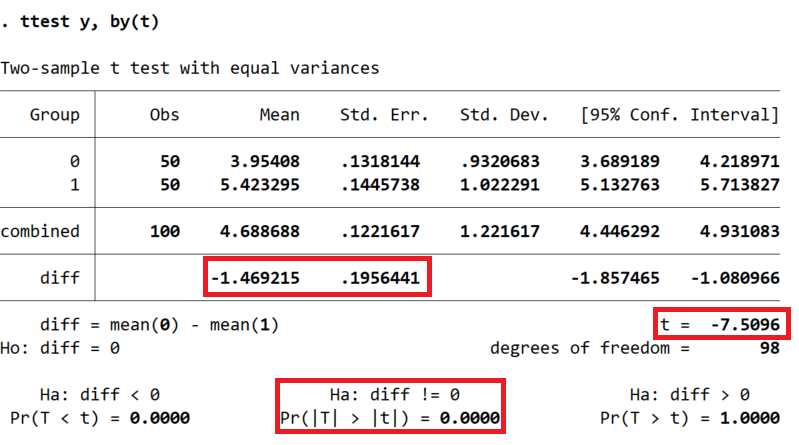
\includegraphics[keepaspectratio,width=6.4cm]{img/stata-ttest2C.png}}};
	
	\node [anchor=north west,align=left,text width = 3.6cm] (text1) at (7,5) {\small{$\textcolor{black}{t } =  \frac{\bar{Y}_T - \bar{Y}_C}{SE \left( \bar{Y}_T - \bar{Y}_C \right) }$}};
	\node [anchor=north west,align=left,text width = 3.6cm] (text2) at (text1.south west) {\small{$\textcolor{white}{t }  =  \frac{ - 1.4692 }{ 0.1956 }$}};
	\node [anchor=north west,align=left,text width = 3.6cm] (text3) at (text2.south west) {\small{$\textcolor{white}{t }  = 7.5096$}};	
	\draw[gray,thick,->] (3.875,3.125) -- (7,4.625);
	\draw[gray,thick,->] (7.25,3.3) -- (6.75,2.75);
	
	\node [red,anchor=north west,align=left,text width = 10cm] (text4) at (0.1,1.25) {\small{To get p-value (in Stata): \texttt{display 2*(1 - abs(ttail(98,-7.5096)))}}};
	
	\end{tikzpicture}
\end{center}
\end{frame}






%%%%%%%%%%%%%%%%%%%%%%%%%%%%%%%%%%%%%%%%%%%%%%%%%%%%%%%%%%%%%%%%%%%%%

\begin{frame}{Testing $H_0: \bar{Y}_T =\bar{Y}_C$ in a Regression}

\medskip
\begin{center}
	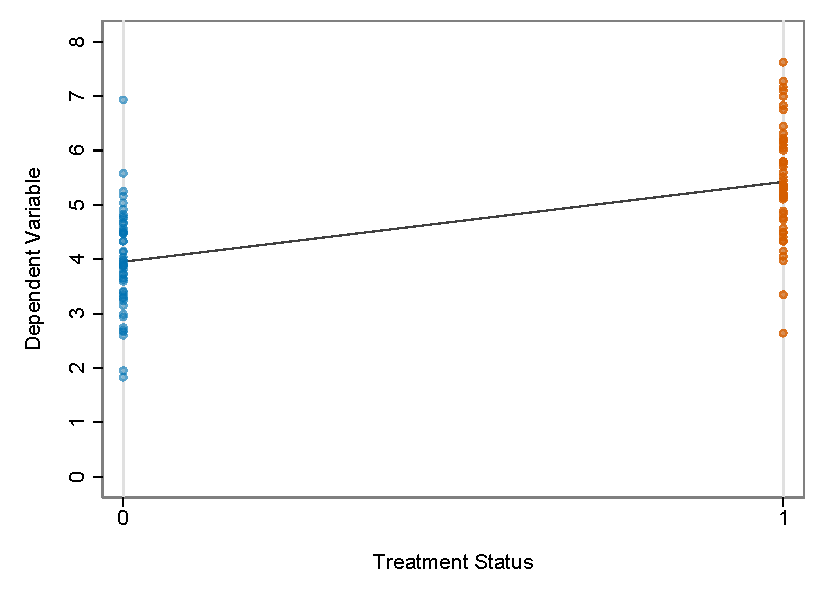
\includegraphics[width=0.54\textwidth]{fig/TvsCreg.pdf}
\end{center}

OLS regression on a binary independent variable: \textcolor{red}{$Y_i = \alpha + \beta D_i + \varepsilon_i$}

\medskip
\begin{itemize}
	
	\item Only two possible predicted values of $\hat{Y_i}$:  $\alpha$ and $\alpha + \beta$
	
\end{itemize}

\end{frame}


%%%%%%%%%%%%%%%%%%%%%%%%%%%%%%%%%%%%%%%%%%%%%%%%%%%%%%%%%%%%%%%%%%%%%

\begin{frame}<handout:0>{OLS Regression on a Binary Independent Variable}

\begin{center}
	\begin{tikzpicture}
	
	% blank canvas
	\only<handout>{\fill[fill=white,draw=white,ultra thin]
		(0,0) -- (11,0) -- (11,6) -- (0,6) -- cycle;}
	\only<beamer>{\fill[fill=white,draw=white,ultra thin]
		(0,0) -- (14,0) -- (14,6) -- (0,6) -- cycle;}
	\only<beamer>{\draw[draw=oiblue!60,fill=oiblue!10,opacity=0.5] (11,1) rectangle (14,5);}
	%\draw[step=1.0,gray!20,thin] (0,0) grid (11,6);
	
	%\pgfmathsetmacro\xshift{3.5cm};
	\pgfmathsetmacro\yshift{-0.75cm};
	
	\node [anchor=base west,align=left,font=\small] (text1A) at (0.25,5.5) {You may or may not remember that in a bivariate regression:};	
	
	\node [anchor=north west,align=left,font=\small] (text2A) at ([yshift=-0.25cm]text1A.south west) {$\hat{\beta}_{OLS}$};
	\node [anchor=base west,align=left,font=\small] (text2B) at (text2A.base east) {$ = $};
	\node [anchor=base west,align=left,font=\small] (text2C) at (text2B.base east) {$\frac{COV (X,Y) }{VAR (X) }$};
	
	%\node [anchor=base,align=left,font=\small] (text3B) at ([yshift=\yshift]text2B.base) {$ = $};
	%\node [red,anchor=base west,align=left,font=\small] (text3C) at (text3B.base east) {$\frac{\sum_i \left( X_i - \bar{X} \right) \left( Y_i - \bar{Y} \right)}{\sum_i \left( X_i - \bar{X} \right)^2 }$};
	
	\end{tikzpicture}
\end{center}

\end{frame}


%%%%%%%%%%%%%%%%%%%%%%%%%%%%%%%%%%%%%%%%%%%%%%%%%%%%%%%%%%%%%%%%%%%%%

\begin{frame}<handout:0>{OLS Regression on a Binary Independent Variable}

\begin{center}
	\begin{tikzpicture}
	
	% blank canvas
	\only<handout>{\fill[fill=white,draw=white,ultra thin]
		(0,0) -- (11,0) -- (11,6) -- (0,6) -- cycle;}
	\only<beamer>{\fill[fill=white,draw=white,ultra thin]
		(0,0) -- (14,0) -- (14,6) -- (0,6) -- cycle;}
	\only<beamer>{\draw[draw=oiblue!60,fill=oiblue!10,opacity=0.5] (11,1) rectangle (14,5);}
	%\draw[step=1.0,gray!20,thin] (0,0) grid (11,6);
	
	%\pgfmathsetmacro\xshift{3.5cm};
	\pgfmathsetmacro\yshift{-0.75cm};
	
	\node [anchor=base west,align=left,font=\small] (text1A) at (0.25,5.5) {You may or may not remember that in a bivariate regression:};	
	
	\node [anchor=north west,align=left,font=\small] (text2A) at ([yshift=-0.25cm]text1A.south west) {$\hat{\beta}_{OLS}$};
	\node [anchor=base west,align=left,font=\small] (text2B) at (text2A.base east) {$ = $};
	\node [anchor=base west,align=left,font=\small] (text2C) at (text2B.base east) {$\frac{COV (X,Y) }{VAR (X) }$};
	
	\node [anchor=base,align=left,font=\small] (text3B) at ([yshift=\yshift]text2B.base) {$ = $};
	\node [red,anchor=base west,align=left,font=\small] (text3C) at (text3B.base east) {$\frac{\sum_i \left( X_i - \bar{X} \right) \left( Y_i - \bar{Y} \right)}{\sum_i \left( X_i - \bar{X} \right)^2 }$};
	
	\end{tikzpicture}
\end{center}

\end{frame}



%%%%%%%%%%%%%%%%%%%%%%%%%%%%%%%%%%%%%%%%%%%%%%%%%%%%%%%%%%%%%%%%%%%%%

\begin{frame}<handout:0>{OLS Regression on a Binary Independent Variable}

\begin{center}
	\begin{tikzpicture}
	
	% blank canvas
	\only<handout>{\fill[fill=white,draw=white,ultra thin]
		(0,0) -- (11,0) -- (11,6) -- (0,6) -- cycle;}
	\only<beamer>{\fill[fill=white,draw=white,ultra thin]
		(0,0) -- (14,0) -- (14,6) -- (0,6) -- cycle;}
	\only<beamer>{\draw[draw=oiblue!60,fill=oiblue!10,opacity=0.5] (11,1) rectangle (14,5);}
	%\draw[step=1.0,gray!20,thin] (0,0) grid (11,6);
	
	%\pgfmathsetmacro\xshift{3.5cm};
	\pgfmathsetmacro\yshift{-0.75cm};
	
	\node [anchor=base west,align=left,font=\small] (text1A) at (0.25,5.5) {You may or may not remember that in a bivariate regression:};	
	
	\node [anchor=north west,align=left,font=\small] (text2A) at ([yshift=-0.25cm]text1A.south west) {$\hat{\beta}_{OLS}$};
	\node [anchor=base west,align=left,font=\small] (text2B) at (text2A.base east) {$ = $};
	\node [anchor=base west,align=left,font=\small] (text2C) at (text2B.base east) {$\frac{COV (X,Y) }{VAR (X) }$};
	
	\node [anchor=base,align=left,font=\small] (text3B) at ([yshift=\yshift]text2B.base) {$ = $};
	\node [anchor=base west,align=left,font=\small] (text3C) at (text3B.base east) {$\frac{\sum_i \left( X_i - \bar{X} \right) \left( Y_i - \bar{Y} \right)}{\sum_i \left( X_i - \bar{X} \right)^2 }$};
	
	\node [anchor=north west,align=left,font=\small] (text4A) at (0.25,3.25) {Notice that the numerator can be re-organized:};
	\node [red,anchor=north west,align=left,font=\footnotesize] (text5A) at ([yshift=-0.125cm]text4A.south west) {$\sum_i \left( X_i - \bar{X} \right) \left( Y_i - \bar{Y} \right)$};
	\node [anchor=base west,align=left,font=\footnotesize] (text5B) at (text5A.base east) {$ = $};
\node [anchor=base west,align=left,font=\footnotesize] (text5C) at (text5B.base east) {$\sum_i  X_i Y_i$};
\node [anchor=base west,align=left,font=\footnotesize] (text5D) at (text5C.base east) {$ - $};
\node [anchor=base west,align=left,font=\footnotesize] (text5E) at (text5D.base east) {$\sum_i \bar{X} Y_i $};
\node [anchor=base west,align=left,font=\footnotesize] (text5F) at (text5E.base east) {$ - $};		
\node [anchor=base west,align=left,font=\footnotesize] (text5G) at (text5F.base east) {$\sum_i \bar{Y} X_i$};
\node [anchor=base west,align=left,font=\footnotesize] (text5H) at (text5G.base east) {$ + $};
\node [,anchor=base west,align=left,font=\footnotesize] (text5I) at (text5H.base east) {$\sum_i  \bar{X} \bar{Y}$};
	
	\end{tikzpicture}
\end{center}

\end{frame}


%%%%%%%%%%%%%%%%%%%%%%%%%%%%%%%%%%%%%%%%%%%%%%%%%%%%%%%%%%%%%%%%%%%%%

\begin{frame}<handout:0>{OLS Regression on a Binary Independent Variable}

\begin{center}
	\begin{tikzpicture}
	
	% blank canvas
	\only<handout>{\fill[fill=white,draw=white,ultra thin]
		(0,0) -- (11,0) -- (11,6) -- (0,6) -- cycle;}
	\only<beamer>{\fill[fill=white,draw=white,ultra thin]
		(0,0) -- (14,0) -- (14,6) -- (0,6) -- cycle;}
	\only<beamer>{\draw[draw=oiblue!60,fill=oiblue!10,opacity=0.5] (11,1) rectangle (14,5);}
	%\draw[step=1.0,gray!20,thin] (0,0) grid (11,6);
	
	%\pgfmathsetmacro\xshift{3.5cm};
	\pgfmathsetmacro\yshift{-0.75cm};
	
	\node [anchor=base west,align=left,font=\small] (text1A) at (0.25,5.5) {You may or may not remember that in a bivariate regression:};	
	
	\node [anchor=north west,align=left,font=\small] (text2A) at ([yshift=-0.25cm]text1A.south west) {$\hat{\beta}_{OLS}$};
	\node [anchor=base west,align=left,font=\small] (text2B) at (text2A.base east) {$ = $};
	\node [anchor=base west,align=left,font=\small] (text2C) at (text2B.base east) {$\frac{COV (X,Y) }{VAR (X) }$};
	
	\node [anchor=base,align=left,font=\small] (text3B) at ([yshift=\yshift]text2B.base) {$ = $};
	\node [anchor=base west,align=left,font=\small] (text3C) at (text3B.base east) {$\frac{\sum_i \left( X_i - \bar{X} \right) \left( Y_i - \bar{Y} \right)}{\sum_i \left( X_i - \bar{X} \right)^2 }$};
	
	\node [anchor=north west,align=left,font=\small] (text4A) at (0.25,3.25) {Notice that the numerator can be re-organized:};
	\node [anchor=north west,align=left,font=\footnotesize] (text5A) at ([yshift=-0.125cm]text4A.south west) {$\sum_i \left( X_i - \bar{X} \right) \left( Y_i - \bar{Y} \right)$};
	\node [anchor=base west,align=left,font=\footnotesize] (text5B) at (text5A.base east) {$ = $};
\node [anchor=base west,align=left,font=\footnotesize] (text5C) at (text5B.base east) {$\sum_i  X_i Y_i$};
\node [anchor=base west,align=left,font=\footnotesize] (text5D) at (text5C.base east) {$ - $};
\node [anchor=base west,align=left,font=\footnotesize] (text5E) at (text5D.base east) {$\sum_i \bar{X} Y_i $};
\node [anchor=base west,align=left,font=\footnotesize] (text5F) at (text5E.base east) {$ - $};		
\node [anchor=base west,align=left,font=\footnotesize] (text5G) at (text5F.base east) {$\sum_i \bar{Y} X_i$};
\node [anchor=base west,align=left,font=\footnotesize] (text5H) at (text5G.base east) {$ + $};
\node [,anchor=base west,align=left,font=\footnotesize] (text5I) at (text5H.base east) {$\sum_i  \bar{X} \bar{Y}$};
	
	\node [red,anchor=north,align=center,font=\footnotesize] (text6G) at ([yshift=-1.25cm]text5G.south) {\textbf{$= \bar{Y} \sum_i X_i$}};
	%\node [red,anchor=base west,align=left,font=\footnotesize] (text6H) at (text6G.base east) {\textbf{$= \bar{Y} N \bar{X} $}};
	\draw [red,->] (text6G.north) -- (text5G.south);
	
	
	\end{tikzpicture}
\end{center}

\end{frame}



%%%%%%%%%%%%%%%%%%%%%%%%%%%%%%%%%%%%%%%%%%%%%%%%%%%%%%%%%%%%%%%%%%%%%

\begin{frame}<handout:0>{OLS Regression on a Binary Independent Variable}

\begin{center}
	\begin{tikzpicture}
	
	% blank canvas
	\only<handout>{\fill[fill=white,draw=white,ultra thin]
		(0,0) -- (11,0) -- (11,6) -- (0,6) -- cycle;}
	\only<beamer>{\fill[fill=white,draw=white,ultra thin]
		(0,0) -- (14,0) -- (14,6) -- (0,6) -- cycle;}
	\only<beamer>{\draw[draw=oiblue!60,fill=oiblue!10,opacity=0.5] (11,1) rectangle (14,5);}
	%\draw[step=1.0,gray!20,thin] (0,0) grid (11,6);
	
	%\pgfmathsetmacro\xshift{3.5cm};
	\pgfmathsetmacro\yshift{-0.75cm};
	
	\node [anchor=base west,align=left,font=\small] (text1A) at (0.25,5.5) {You may or may not remember that in a bivariate regression:};	
	
	\node [anchor=north west,align=left,font=\small] (text2A) at ([yshift=-0.25cm]text1A.south west) {$\hat{\beta}_{OLS}$};
	\node [anchor=base west,align=left,font=\small] (text2B) at (text2A.base east) {$ = $};
	\node [anchor=base west,align=left,font=\small] (text2C) at (text2B.base east) {$\frac{COV (X,Y) }{VAR (X) }$};
	
	\node [anchor=base,align=left,font=\small] (text3B) at ([yshift=\yshift]text2B.base) {$ = $};
	\node [anchor=base west,align=left,font=\small] (text3C) at (text3B.base east) {$\frac{\sum_i \left( X_i - \bar{X} \right) \left( Y_i - \bar{Y} \right)}{\sum_i \left( X_i - \bar{X} \right)^2 }$};
	
	\node [anchor=north west,align=left,font=\small] (text4A) at (0.25,3.25) {Notice that the numerator can be re-organized:};
	\node [anchor=north west,align=left,font=\footnotesize] (text5A) at ([yshift=-0.125cm]text4A.south west) {$\sum_i \left( X_i - \bar{X} \right) \left( Y_i - \bar{Y} \right)$};
	\node [anchor=base west,align=left,font=\footnotesize] (text5B) at (text5A.base east) {$ = $};
\node [anchor=base west,align=left,font=\footnotesize] (text5C) at (text5B.base east) {$\sum_i  X_i Y_i$};
\node [anchor=base west,align=left,font=\footnotesize] (text5D) at (text5C.base east) {$ - $};
\node [anchor=base west,align=left,font=\footnotesize] (text5E) at (text5D.base east) {$\sum_i \bar{X} Y_i $};
\node [anchor=base west,align=left,font=\footnotesize] (text5F) at (text5E.base east) {$ - $};		
\node [anchor=base west,align=left,font=\footnotesize] (text5G) at (text5F.base east) {$\sum_i \bar{Y} X_i$};
\node [anchor=base west,align=left,font=\footnotesize] (text5H) at (text5G.base east) {$ + $};
\node [,anchor=base west,align=left,font=\footnotesize] (text5I) at (text5H.base east) {$\sum_i  \bar{X} \bar{Y}$};
	
	\node [red,anchor=north,align=center,font=\footnotesize] (text6G) at ([yshift=-1.25cm]text5G.south) {\textbf{$= \bar{Y} \sum_i X_i$}};
	\node [red,anchor=base west,align=left,font=\footnotesize] (text6H) at (text6G.base east) {\textbf{$= \bar{Y} N \bar{X} $}};
	\draw [red,->] (text6G.north) -- (text5G.south);

	
	\end{tikzpicture}
\end{center}

\end{frame}




%%%%%%%%%%%%%%%%%%%%%%%%%%%%%%%%%%%%%%%%%%%%%%%%%%%%%%%%%%%%%%%%%%%%%

\begin{frame}<handout:0>{OLS Regression on a Binary Independent Variable}

\begin{center}
	\begin{tikzpicture}
	
	% blank canvas
	\only<handout>{\fill[fill=white,draw=white,ultra thin]
		(0,0) -- (11,0) -- (11,6) -- (0,6) -- cycle;}
	\only<beamer>{\fill[fill=white,draw=white,ultra thin]
		(0,0) -- (14,0) -- (14,6) -- (0,6) -- cycle;}
	\only<beamer>{\draw[draw=oiblue!60,fill=oiblue!10,opacity=0.5] (11,1) rectangle (14,5);}
	%\draw[step=1.0,gray!20,thin] (0,0) grid (11,6);
	
	%\pgfmathsetmacro\xshift{3.5cm};
	\pgfmathsetmacro\yshift{-0.75cm};
	
	\node [anchor=base west,align=left,font=\small] (text1A) at (0.25,5.5) {You may or may not remember that in a bivariate regression:};	
	
	\node [anchor=north west,align=left,font=\small] (text2A) at ([yshift=-0.25cm]text1A.south west) {$\hat{\beta}_{OLS}$};
	\node [anchor=base west,align=left,font=\small] (text2B) at (text2A.base east) {$ = $};
	\node [anchor=base west,align=left,font=\small] (text2C) at (text2B.base east) {$\frac{COV (X,Y) }{VAR (X) }$};
	
	\node [anchor=base,align=left,font=\small] (text3B) at ([yshift=\yshift]text2B.base) {$ = $};
	\node [anchor=base west,align=left,font=\small] (text3C) at (text3B.base east) {$\frac{\sum_i \left( X_i - \bar{X} \right) \left( Y_i - \bar{Y} \right)}{\sum_i \left( X_i - \bar{X} \right)^2 }$};
	
	\node [anchor=north west,align=left,font=\small] (text4A) at (0.25,3.25) {Notice that the numerator can be re-organized:};
	\node [anchor=north west,align=left,font=\footnotesize] (text5A) at ([yshift=-0.125cm]text4A.south west) {$\sum_i \left( X_i - \bar{X} \right) \left( Y_i - \bar{Y} \right)$};
	\node [anchor=base west,align=left,font=\footnotesize] (text5B) at (text5A.base east) {$ = $};
\node [anchor=base west,align=left,font=\footnotesize] (text5C) at (text5B.base east) {$\sum_i  X_i Y_i$};
\node [anchor=base west,align=left,font=\footnotesize] (text5D) at (text5C.base east) {$ - $};
\node [anchor=base west,align=left,font=\footnotesize] (text5E) at (text5D.base east) {$\sum_i \bar{X} Y_i $};
\node [anchor=base west,align=left,font=\footnotesize] (text5F) at (text5E.base east) {$ - $};		
\node [anchor=base west,align=left,font=\footnotesize] (text5G) at (text5F.base east) {$\sum_i \bar{Y} X_i$};
\node [anchor=base west,align=left,font=\footnotesize] (text5H) at (text5G.base east) {$ + $};
\node [,anchor=base west,align=left,font=\footnotesize] (text5I) at (text5H.base east) {$\sum_i  \bar{X} \bar{Y}$};
	
	\node [gray,anchor=north,align=center,font=\footnotesize] (text6G) at ([yshift=-1.25cm]text5G.south) {\textbf{$= \bar{Y} \sum_i X_i$}};
	\node [gray,anchor=base west,align=left,font=\footnotesize] (text6H) at (text6G.base east) {\textbf{$= \bar{Y} N \bar{X} $}};
	\draw [gray,->] (text6G.north) -- (text5G.south);
	
	\node [red,anchor=north,align=center,font=\footnotesize] (text6I) at ([yshift=-0.25cm]text5I.south) {\textbf{$= N \bar{X} \bar{Y} $}};
	\draw [red,->] (text6I.north) -- (text5I.south);
	
	%\draw [gray,<->] (text6I.south) -- (text6H.north) node [red,pos=0.5] {$=$};
	%\draw [gray,<->] (text6I.south) -- (text6H.north) ;
	
	\end{tikzpicture}
\end{center}

\end{frame}



%%%%%%%%%%%%%%%%%%%%%%%%%%%%%%%%%%%%%%%%%%%%%%%%%%%%%%%%%%%%%%%%%%%%%

\begin{frame}{OLS Regression on a Binary Independent Variable}

\begin{center}
	\begin{tikzpicture}
	
	% blank canvas
	\only<handout>{\fill[fill=white,draw=white,ultra thin]
		(0,0) -- (11,0) -- (11,6) -- (0,6) -- cycle;}
	\only<beamer>{\fill[fill=white,draw=white,ultra thin]
		(0,0) -- (14,0) -- (14,6) -- (0,6) -- cycle;}
	\only<beamer>{\draw[draw=oiblue!60,fill=oiblue!10,opacity=0.5] (11,1) rectangle (14,5);}
	%\draw[step=1.0,gray!20,thin] (0,0) grid (11,6);
	
	%\pgfmathsetmacro\xshift{3.5cm};
	\pgfmathsetmacro\yshift{-0.75cm};
	
	\node [anchor=base west,align=left,font=\small] (text1A) at (0.25,5.5) {You may or may not remember that in a bivariate regression:};	
	
	\node [anchor=north west,align=left,font=\small] (text2A) at ([yshift=-0.25cm]text1A.south west) {$\hat{\beta}_{OLS}$};
	\node [anchor=base west,align=left,font=\small] (text2B) at (text2A.base east) {$ = $};
	\node [anchor=base west,align=left,font=\small] (text2C) at (text2B.base east) {$\frac{COV (X,Y) }{VAR (X) }$};
	
	\node [anchor=base,align=left,font=\small] (text3B) at ([yshift=\yshift]text2B.base) {$ = $};
	\node [anchor=base west,align=left,font=\small] (text3C) at (text3B.base east) {$\frac{\sum_i \left( X_i - \bar{X} \right) \left( Y_i - \bar{Y} \right)}{\sum_i \left( X_i - \bar{X} \right)^2 }$};
	
	\node [anchor=north west,align=left,font=\small] (text4A) at (0.25,3.25) {Notice that the numerator can be re-organized:};
	\node [anchor=north west,align=left,font=\footnotesize] (text5A) at ([yshift=-0.125cm]text4A.south west) {$\sum_i \left( X_i - \bar{X} \right) \left( Y_i - \bar{Y} \right)$};
	\node [anchor=base west,align=left,font=\footnotesize] (text5B) at (text5A.base east) {$ = $};
\node [anchor=base west,align=left,font=\footnotesize] (text5C) at (text5B.base east) {$\sum_i  X_i Y_i$};
\node [anchor=base west,align=left,font=\footnotesize] (text5D) at (text5C.base east) {$ - $};
\node [anchor=base west,align=left,font=\footnotesize] (text5E) at (text5D.base east) {$\sum_i \bar{X} Y_i $};
\node [anchor=base west,align=left,font=\footnotesize] (text5F) at (text5E.base east) {$ - $};		
\node [anchor=base west,align=left,font=\footnotesize] (text5G) at (text5F.base east) {$\sum_i \bar{Y} X_i$};
\node [anchor=base west,align=left,font=\footnotesize] (text5H) at (text5G.base east) {$ + $};
\node [,anchor=base west,align=left,font=\footnotesize] (text5I) at (text5H.base east) {$\sum_i  \bar{X} \bar{Y}$};
	
	\node [anchor=north,align=center,font=\footnotesize] (text6G) at ([yshift=-1.25cm]text5G.south) {\textbf{$= \bar{Y} \sum_i X_i$}};
	\node [red,anchor=base west,align=left,font=\footnotesize] (text6H) at (text6G.base east) {\textbf{$= \bar{Y} N \bar{X} $}};
	\draw [gray,->] (text6G.north) -- (text5G.south);

	\node [red,anchor=north,align=center,font=\footnotesize] (text6I) at ([yshift=-0.25cm]text5I.south) {\textbf{$= N \bar{X} \bar{Y} $}};
	\draw [gray,->] (text6I.north) -- (text5I.south);
	
	%\draw [gray,<->] (text6I.south) -- (text6H.north) node [red,pos=0.5] {$=$};
	\draw [red,<->,ultra thin,double distance=0.6pt] ([xshift=0.125cm]text6I.south) -- ([xshift=0.25cm]text6H.north) ;
		
	\end{tikzpicture}
\end{center}

\end{frame}



%%%%%%%%%%%%%%%%%%%%%%%%%%%%%%%%%%%%%%%%%%%%%%%%%%%%%%%%%%%%%%%%%%%%%

\begin{frame}<handout:0>{OLS Regression on a Binary Independent Variable}

\begin{center}
	\begin{tikzpicture}
	
	% blank canvas
	\only<handout>{\fill[fill=white,draw=white,ultra thin]
		(0,0) -- (11,0) -- (11,6) -- (0,6) -- cycle;}
	\only<beamer>{\fill[fill=white,draw=white,ultra thin]
		(0,0) -- (14,0) -- (14,6) -- (0,6) -- cycle;}
	\only<beamer>{\draw[draw=oiblue!60,fill=oiblue!10,opacity=0.5] (11,1) rectangle (14,5);}
	%\draw[step=1.0,gray!20,thin] (0,0) grid (11,6);
	
	%\pgfmathsetmacro\xshift{3.5cm};
	\pgfmathsetmacro\yshift{-0.75cm};
	
	\node [anchor=base west,align=left,font=\small] (text1A) at (0.25,5.5) {You may or may not remember that in a bivariate regression:};	
	
	\node [anchor=north west,align=left,font=\small] (text2A) at ([yshift=-0.25cm]text1A.south west) {$\hat{\beta}_{OLS}$};
	\node [anchor=base west,align=left,font=\small] (text2B) at (text2A.base east) {$ = $};
	\node [anchor=base west,align=left,font=\small] (text2C) at (text2B.base east) {$\frac{COV (X,Y) }{VAR (X) }$};
	
	\node [anchor=base,align=left,font=\small] (text3B) at ([yshift=\yshift]text2B.base) {$ = $};
	\node [anchor=base west,align=left,font=\small] (text3C) at (text3B.base east) {$\frac{\sum_i \left( X_i - \bar{X} \right) \left( Y_i - \bar{Y} \right)}{\sum_i \left( X_i - \bar{X} \right)^2 }$};
	
	\node [anchor=north west,align=left,font=\small] (text4A) at (0.25,3.25) {Notice that the numerator can be re-organized:};
	\node [anchor=north west,align=left,font=\footnotesize] (text5A) at ([yshift=-0.125cm]text4A.south west) {$\sum_i \left( X_i - \bar{X} \right) \left( Y_i - \bar{Y} \right)$};
	\node [anchor=base west,align=left,font=\footnotesize] (text5B) at (text5A.base east) {$ = $};
\node [anchor=base west,align=left,font=\footnotesize] (text5C) at (text5B.base east) {$\sum_i  X_i Y_i$};
\node [anchor=base west,align=left,font=\footnotesize] (text5D) at (text5C.base east) {$ - $};
\node [anchor=base west,align=left,font=\footnotesize] (text5E) at (text5D.base east) {$\sum_i \bar{X} Y_i $};
%	\node [anchor=base west,align=left,font=\footnotesize] (text5F) at (text5E.base east) {$ - $};		
%	\node [anchor=base west,align=left,font=\footnotesize] (text5G) at (text5F.base east) {$\sum_i \bar{Y} X_i$};
%	\node [anchor=base west,align=left,font=\footnotesize] (text5H) at (text5G.base east) {$ + $};
%	\node [,anchor=base west,align=left,font=\footnotesize] (text5I) at (text5H.base east) {$\sum_i  \bar{X} \bar{Y}$};
	
	\end{tikzpicture}
\end{center}

\end{frame}


%%%%%%%%%%%%%%%%%%%%%%%%%%%%%%%%%%%%%%%%%%%%%%%%%%%%%%%%%%%%%%%%%%%%%

\begin{frame}<handout:0>{OLS Regression on a Binary Independent Variable}

\begin{center}
	\begin{tikzpicture}
	
	% blank canvas
	\only<handout>{\fill[fill=white,draw=white,ultra thin]
		(0,0) -- (11,0) -- (11,6) -- (0,6) -- cycle;}
	\only<beamer>{\fill[fill=white,draw=white,ultra thin]
		(0,0) -- (14,0) -- (14,6) -- (0,6) -- cycle;}
	\only<beamer>{\draw[draw=oiblue!60,fill=oiblue!10,opacity=0.5] (11,1) rectangle (14,5);}
	%\draw[step=1.0,gray!20,thin] (0,0) grid (11,6);
	
	%\pgfmathsetmacro\xshift{3.5cm};
	\pgfmathsetmacro\yshift{-0.75cm};
	
	\node [anchor=base west,align=left,font=\small] (text1A) at (0.25,5.5) {You may or may not remember that in a bivariate regression:};	
	
	\node [anchor=north west,align=left,font=\small] (text2A) at ([yshift=-0.25cm]text1A.south west) {$\hat{\beta}_{OLS}$};
	\node [anchor=base west,align=left,font=\small] (text2B) at (text2A.base east) {$ = $};
	\node [anchor=base west,align=left,font=\small] (text2C) at (text2B.base east) {$\frac{COV (X,Y) }{VAR (X) }$};
	
	\node [anchor=base,align=left,font=\small] (text3B) at ([yshift=\yshift]text2B.base) {$ = $};
	\node [anchor=base west,align=left,font=\small] (text3C) at (text3B.base east) {$\frac{\sum_i \left( X_i - \bar{X} \right) \left( Y_i - \bar{Y} \right)}{\sum_i \left( X_i - \bar{X} \right)^2 }$};
	
	\node [anchor=north west,align=left,font=\small] (text4A) at (0.25,3.25) {Notice that the numerator can be re-organized:};
	\node [anchor=north west,align=left,font=\footnotesize] (text5A) at ([yshift=-0.125cm]text4A.south west) {$\sum_i \left( X_i - \bar{X} \right) \left( Y_i - \bar{Y} \right)$};
	\node [anchor=base west,align=left,font=\footnotesize] (text5B) at (text5A.base east) {$ = $};
\node [anchor=base west,align=left,font=\footnotesize] (text5C) at (text5B.base east) {$\sum_i  X_i Y_i$};
\node [anchor=base west,align=left,font=\footnotesize] (text5D) at (text5C.base east) {$ - $};
\node [anchor=base west,align=left,font=\footnotesize] (text5E) at (text5D.base east) {$\sum_i \bar{X} Y_i $};
%	\node [anchor=base west,align=left,font=\footnotesize] (text5F) at (text5E.base east) {$ - $};		
%	\node [anchor=base west,align=left,font=\footnotesize] (text5G) at (text5F.base east) {$\sum_i \bar{Y} X_i$};
%	\node [anchor=base west,align=left,font=\footnotesize] (text5H) at (text5G.base east) {$ + $};
%	\node [,anchor=base west,align=left,font=\footnotesize] (text5I) at (text5H.base east) {$\sum_i  \bar{X} \bar{Y}$};
	
	\node [anchor=base east,align=left,font=\footnotesize] (text6B) at ([yshift=\yshift]text5B.base east) {$ = $};
	\node [red,anchor=base west,align=left,font=\footnotesize] (text6C) at (text6B.base east) {\textbf{$\sum_i \left[ Y_i \left( X_i - \bar{X} \right) \right] $}};	
	
	\end{tikzpicture}
\end{center}

\end{frame}



%%%%%%%%%%%%%%%%%%%%%%%%%%%%%%%%%%%%%%%%%%%%%%%%%%%%%%%%%%%%%%%%%%%%%

\begin{frame}{OLS Regression on a Binary Independent Variable}

\begin{center}
	\begin{tikzpicture}
	
	% blank canvas
	\only<handout>{\fill[fill=white,draw=white,ultra thin]
		(0,0) -- (11,0) -- (11,6) -- (0,6) -- cycle;}
	\only<beamer>{\fill[fill=white,draw=white,ultra thin]
		(0,0) -- (14,0) -- (14,6) -- (0,6) -- cycle;}
	\only<beamer>{\draw[draw=oiblue!60,fill=oiblue!10,opacity=0.5] (11,1) rectangle (14,5);}
	%\draw[step=1.0,gray!20,thin] (0,0) grid (11,6);
	
	%\pgfmathsetmacro\xshift{3.5cm};
	\pgfmathsetmacro\yshift{-0.75cm};
	
	\node [anchor=base west,align=left,font=\small] (text1A) at (0.25,5.5) {You may or may not remember that in a bivariate regression:};	
	
	\node [anchor=north west,align=left,font=\small] (text2A) at ([yshift=-0.25cm]text1A.south west) {$\hat{\beta}_{OLS}$};
	\node [anchor=base west,align=left,font=\small] (text2B) at (text2A.base east) {$ = $};
	\node [anchor=base west,align=left,font=\small] (text2C) at (text2B.base east) {$\frac{COV (X,Y) }{VAR (X) }$};
	
	\node [anchor=base,align=left,font=\small] (text3B) at ([yshift=\yshift]text2B.base) {$ = $};
	\node [anchor=base west,align=left,font=\small] (text3C) at (text3B.base east) {$\frac{\sum_i \left( X_i - \bar{X} \right) \left( Y_i - \bar{Y} \right)}{\sum_i \left( X_i - \bar{X} \right)^2 }$};
	
	\node [anchor=north west,align=left,font=\small] (text4A) at (0.25,3.25) {Notice that the numerator can be re-organized:};
	\node [anchor=north west,align=left,font=\footnotesize] (text5A) at ([yshift=-0.125cm]text4A.south west) {$\sum_i \left( X_i - \bar{X} \right) \left( Y_i - \bar{Y} \right)$};
	\node [anchor=base west,align=left,font=\footnotesize] (text5B) at (text5A.base east) {$ = $};
	\node [anchor=base west,align=left,font=\footnotesize] (text5C) at (text5B.base east) {$\sum_i  X_i Y_i$};
	\node [anchor=base west,align=left,font=\footnotesize] (text5D) at (text5C.base east) {$ - $};
	\node [anchor=base west,align=left,font=\footnotesize] (text5E) at (text5D.base east) {$\sum_i \bar{X} Y_i $};
	%	\node [anchor=base west,align=left,font=\footnotesize] (text5F) at (text5E.base east) {$ - $};		
	%	\node [anchor=base west,align=left,font=\footnotesize] (text5G) at (text5F.base east) {$\sum_i \bar{Y} X_i$};
	%	\node [anchor=base west,align=left,font=\footnotesize] (text5H) at (text5G.base east) {$ + $};
	%	\node [,anchor=base west,align=left,font=\footnotesize] (text5I) at (text5H.base east) {$\sum_i  \bar{X} \bar{Y}$};
	
	\node [anchor=base east,align=left,font=\footnotesize] (text6B) at ([yshift=\yshift]text5B.base east) {$ = $};
	\node [red,anchor=base west,align=left,font=\footnotesize] (text6C) at (text6B.base east) {\textbf{$\sum_i \left[ Y_i \left( X_i - \bar{X} \right) \right] $}};	
	\draw [red,->] (text6C.mid east) .. controls +(4,1.5) and ([xshift=3cm]text3C.mid east) .. (text3C.mid east); 

	
	\end{tikzpicture}
\end{center}

\end{frame}



%%%%%%%%%%%%%%%%%%%%%%%%%%%%%%%%%%%%%%%%%%%%%%%%%%%%%%%%%%%%%%%%%%%%%

\begin{frame}<handout:0>{OLS Regression on a Binary Independent Variable}

\begin{center}
	\begin{tikzpicture}
	
	% blank canvas
	\only<handout>{\fill[fill=white,draw=white,ultra thin]
		(0,0) -- (11,0) -- (11,6) -- (0,6) -- cycle;}
	\only<beamer>{\fill[fill=white,draw=white,ultra thin]
		(0,0) -- (14,0) -- (14,6) -- (0,6) -- cycle;}
	\only<beamer>{\draw[draw=oiblue!60,fill=oiblue!10,opacity=0.5] (11,1) rectangle (14,5);}
	%\draw[step=1.0,gray!20,thin] (0,0) grid (11,6);
	
	%\pgfmathsetmacro\xshift{3.5cm};
	\pgfmathsetmacro\yshift{-0.75cm};
	
	\node [anchor=base west,align=left,font=\small] (text1A) at (0.25,5.5) {You may or may not remember that in a bivariate regression:};	
	
	\node [anchor=north west,align=left,font=\small] (text2A) at ([yshift=-0.25cm]text1A.south west) {$\hat{\beta}_{OLS}$};
	\node [anchor=base west,align=left,font=\small] (text2B) at (text2A.base east) {$ = $};
	\node [anchor=base west,align=left,font=\small] (text2C) at (text2B.base east) {$\frac{COV (X,Y) }{VAR (X) }$};
	
	\node [anchor=base,align=left,font=\small] (text3B) at ([yshift=\yshift]text2B.base) {$ = $};
	\node [anchor=base west,align=left,font=\small] (text3C) at (text3B.base east) {$\frac{\sum_i \left[ Y_i \left( X_i - \bar{X} \right) \right]}{\sum_i \left( X_i - \bar{X} \right)^2 }$};
	
%	\node [anchor=base,align=left,font=\small] (text4B) at ([yshift=\yshift]text3B.base) {$ = $};
%	\node [anchor=base west,align=left,font=\small] (text4C) at (text4B.base east) {$\frac{\sum_i \left[ Y_i \left( X_i - \bar{X} \right) \right] }{\sum_i \left( X_i - \bar{X} \right)^2 }$};	
	
	\end{tikzpicture}
\end{center}

\end{frame}





%%%%%%%%%%%%%%%%%%%%%%%%%%%%%%%%%%%%%%%%%%%%%%%%%%%%%%%%%%%%%%%%%%%%%

\begin{frame}<handout:0>{OLS Regression on a Binary Independent Variable}

\begin{center}
	\begin{tikzpicture}
	
	% blank canvas
	\only<handout>{\fill[fill=white,draw=white,ultra thin]
		(0,0) -- (11,0) -- (11,6) -- (0,6) -- cycle;}
	\only<beamer>{\fill[fill=white,draw=white,ultra thin]
		(0,0) -- (14,0) -- (14,6) -- (0,6) -- cycle;}
	\only<beamer>{\draw[draw=oiblue!60,fill=oiblue!10,opacity=0.5] (11,1) rectangle (14,5);}
	%\draw[step=1.0,gray!20,thin] (0,0) grid (11,6);
	
	%\pgfmathsetmacro\xshift{3.5cm};
	\pgfmathsetmacro\yshift{-0.75cm};
	
	\node [anchor=base west,align=left,font=\small] (text1A) at (0.25,5.5) {You may or may not remember that in a bivariate regression:};	
	
	\node [anchor=north west,align=left,font=\small] (text2A) at ([yshift=-0.25cm]text1A.south west) {$\hat{\beta}_{OLS}$};
	\node [anchor=base west,align=left,font=\small] (text2B) at (text2A.base east) {$ = $};
	\node [anchor=base west,align=left,font=\small] (text2C) at (text2B.base east) {$\frac{COV (X,Y) }{VAR (X) }$};
	
	\node [anchor=base,align=left,font=\small] (text3B) at ([yshift=\yshift]text2B.base) {$ = $};
	\node [anchor=base west,align=left,font=\small] (text3C) at (text3B.base east) {$\frac{\sum_i \left[ Y_i \left( X_i - \bar{X} \right) \right]}{\sum_i \left( X_i - \bar{X} \right)^2 }$};
	
	\node [red,anchor=north west,align=left,font=\small] (text4A) at (4,5) {When independent variable is binary:};
	\node [red,anchor=north west,align=left,font=\footnotesize] (text5A) at (text4A.south west) {$\bar{X} $};
	\node [red,anchor=base west,align=left,font=\footnotesize] (text5B) at (text5A.base east) {$ = $};
	\node [red,anchor=base west,align=left,font=\footnotesize] (text5C) at (text5B.base east) {$\frac{n_T}{N}$};
	\node [red,anchor=base west,align=left,font=\footnotesize] (text5D) at (text5C.base east) {($n_T$ is \# of treated observations)};

	%\node [anchor=base east,align=left,font=\footnotesize] (text6B) at ([yshift=\yshift]text5B.base east) {$ \Rightarrow $};
	%\node [anchor=base west,align=left,font=\footnotesize] (text6C) at (text6B.base east) {$X_i - \bar{X} = 1 - \frac{n_T}{N}$ if $D_i = 1$; $X_i - \bar{X} = - \frac{n_T}{N}$ otherwise};
	%\node [anchor=base west,align=left,font=\footnotesize] (text6D) at (text6C.base east) {(where $n_T$ is number of treated observations)};
	
	\end{tikzpicture}
\end{center}

\end{frame}




%%%%%%%%%%%%%%%%%%%%%%%%%%%%%%%%%%%%%%%%%%%%%%%%%%%%%%%%%%%%%%%%%%%%%

\begin{frame}<handout:0>{OLS Regression on a Binary Independent Variable}

\begin{center}
	\begin{tikzpicture}
	
	% blank canvas
	\only<handout>{\fill[fill=white,draw=white,ultra thin]
		(0,0) -- (11,0) -- (11,6) -- (0,6) -- cycle;}
	\only<beamer>{\fill[fill=white,draw=white,ultra thin]
		(0,0) -- (14,0) -- (14,6) -- (0,6) -- cycle;}
	\only<beamer>{\draw[draw=oiblue!60,fill=oiblue!10,opacity=0.5] (11,1) rectangle (14,5);}
	%\draw[step=1.0,gray!20,thin] (0,0) grid (11,6);
	
	%\pgfmathsetmacro\xshift{3.5cm};
	\pgfmathsetmacro\yshift{-0.75cm};
	
	\node [anchor=base west,align=left,font=\small] (text1A) at (0.25,5.5) {You may or may not remember that in a bivariate regression:};	
	
	\node [anchor=north west,align=left,font=\small] (text2A) at ([yshift=-0.25cm]text1A.south west) {$\hat{\beta}_{OLS}$};
	\node [anchor=base west,align=left,font=\small] (text2B) at (text2A.base east) {$ = $};
	\node [anchor=base west,align=left,font=\small] (text2C) at (text2B.base east) {$\frac{COV (X,Y) }{VAR (X) }$};
	
	\node [anchor=base,align=left,font=\small] (text3B) at ([yshift=\yshift]text2B.base) {$ = $};
	\node [anchor=base west,align=left,font=\small] (text3C) at (text3B.base east) {$\frac{\sum_i \left[ Y_i \left( X_i - \bar{X} \right) \right]}{\sum_i \left( X_i - \bar{X} \right)^2 }$};
	
	\node [gray,anchor=north west,align=left,font=\small] (text4A) at (4,5) {When independent variable is binary:};
	\node [gray,anchor=north west,align=left,font=\footnotesize] (text5A) at (text4A.south west) {$\bar{X} $};
	\node [gray,anchor=base west,align=left,font=\footnotesize] (text5B) at (text5A.base east) {$ = $};
	\node [gray,anchor=base west,align=left,font=\footnotesize] (text5C) at (text5B.base east) {$\frac{n_T}{N}$};
	\node [gray,anchor=base west,align=left,font=\footnotesize] (text5D) at (text5C.base east) {($n_T$ is \# of treated observations)};
	
	\node [red,anchor=north west,align=left,font=\small] (text6A) at ([yshift=-0.75cm]text4A.south west) {Assume observations are ordered:};
	
	\node [red,anchor=north west,align=left,font=\footnotesize] (text7A) at (text6A.south west) {$\big\{$};
	
	\node [red,anchor=base west,align=left,font=\footnotesize] (text7C) at ([xshift=-0.25cm]text7A.base east) {$Y_1 , Y_2 , \ldots , Y_{n_{T-1}}  , Y_{n_T} $};
	\draw[white,snake=brace,mirror snake,gap around snake=0.125cm,raise snake=-2pt] (text7C.south west) -- (text7C.south east) node[pos=0.5,anchor=north,align=center,font=\scriptsize] {treatment group};
	
	\node [red,anchor=base west,align=left,font=\footnotesize] (text7D) at ([xshift=-0.25cm]text7C.base east) {$, $};
	
	\node [red,anchor=base west,align=left,font=\footnotesize] (text7E) at ([xshift=-0.25cm]text7D.base east) {$Y_{n_{T+1}} , Y_{n_{T+2}} , \ldots , Y_{N}$};
	\draw[white,snake=brace,mirror snake,gap around snake=0.125cm,raise snake=-2pt] (text7E.south west) -- (text7E.south east) node[pos=0.5,anchor=north,align=center,font=\scriptsize] {control group};
	
	\node [red,anchor=base west,align=left,font=\footnotesize] (text7F) at ([xshift=-0.25cm]text7E.base east) {$\big\}$};
	
	\end{tikzpicture}
\end{center}

\end{frame}



%%%%%%%%%%%%%%%%%%%%%%%%%%%%%%%%%%%%%%%%%%%%%%%%%%%%%%%%%%%%%%%%%%%%%

\begin{frame}<handout:0>{OLS Regression on a Binary Independent Variable}

\begin{center}
	\begin{tikzpicture}
	
	% blank canvas
	\only<handout>{\fill[fill=white,draw=white,ultra thin]
		(0,0) -- (11,0) -- (11,6) -- (0,6) -- cycle;}
	\only<beamer>{\fill[fill=white,draw=white,ultra thin]
		(0,0) -- (14,0) -- (14,6) -- (0,6) -- cycle;}
	\only<beamer>{\draw[draw=oiblue!60,fill=oiblue!10,opacity=0.5] (11,1) rectangle (14,5);}
	%\draw[step=1.0,gray!20,thin] (0,0) grid (11,6);
	
	%\pgfmathsetmacro\xshift{3.5cm};
	\pgfmathsetmacro\yshift{-0.75cm};
	
	\node [anchor=base west,align=left,font=\small] (text1A) at (0.25,5.5) {You may or may not remember that in a bivariate regression:};	
	
	\node [anchor=north west,align=left,font=\small] (text2A) at ([yshift=-0.25cm]text1A.south west) {$\hat{\beta}_{OLS}$};
	\node [anchor=base west,align=left,font=\small] (text2B) at (text2A.base east) {$ = $};
	\node [anchor=base west,align=left,font=\small] (text2C) at (text2B.base east) {$\frac{COV (X,Y) }{VAR (X) }$};
	
	\node [anchor=base,align=left,font=\small] (text3B) at ([yshift=\yshift]text2B.base) {$ = $};
	\node [anchor=base west,align=left,font=\small] (text3C) at (text3B.base east) {$\frac{\sum_i \left[ Y_i \left( X_i - \bar{X} \right) \right]}{\sum_i \left( X_i - \bar{X} \right)^2 }$};
	
	\node [gray,anchor=north west,align=left,font=\small] (text4A) at (4,5) {When independent variable is binary:};
	\node [gray,anchor=north west,align=left,font=\footnotesize] (text5A) at (text4A.south west) {$\bar{X} $};
	\node [gray,anchor=base west,align=left,font=\footnotesize] (text5B) at (text5A.base east) {$ = $};
	\node [gray,anchor=base west,align=left,font=\footnotesize] (text5C) at (text5B.base east) {$\frac{n_T}{N}$};
	\node [gray,anchor=base west,align=left,font=\footnotesize] (text5D) at (text5C.base east) {($n_T$ is \# of treated observations)};
	
	\node [anchor=north west,align=left,font=\small] (text6A) at ([yshift=-0.75cm]text4A.south west) {Assume observations are ordered:};
	
	\node [anchor=north west,align=left,font=\footnotesize] (text7A) at (text6A.south west) {$\big\{$};
	
	\node [red,anchor=base west,align=left,font=\footnotesize] (text7C) at ([xshift=-0.25cm]text7A.base east) {$Y_1 , Y_2 , \ldots , Y_{n_{T-1}}  , Y_{n_T} $};
	\draw[red,snake=brace,mirror snake,gap around snake=0.125cm,raise snake=-2pt] (text7C.south west) -- (text7C.south east) node[pos=0.5,anchor=north,align=center,font=\scriptsize] {treatment group};
	
	\node [anchor=base west,align=left,font=\footnotesize] (text7D) at ([xshift=-0.25cm]text7C.base east) {$, $};
	
	\node [anchor=base west,align=left,font=\footnotesize] (text7E) at ([xshift=-0.25cm]text7D.base east) {$Y_{n_{T+1}} , Y_{n_{T+2}} , \ldots , Y_{N}$};
	\draw[white,snake=brace,mirror snake,gap around snake=0.125cm,raise snake=-2pt] (text7E.south west) -- (text7E.south east) node[pos=0.5,anchor=north,align=center,font=\scriptsize] {control group};
	
	\node [anchor=base west,align=left,font=\footnotesize] (text7F) at ([xshift=-0.25cm]text7E.base east) {$\big\}$};
	
	\end{tikzpicture}
\end{center}

\end{frame}



%%%%%%%%%%%%%%%%%%%%%%%%%%%%%%%%%%%%%%%%%%%%%%%%%%%%%%%%%%%%%%%%%%%%%

\begin{frame}<handout:0>{OLS Regression on a Binary Independent Variable}

\begin{center}
	\begin{tikzpicture}
	
	% blank canvas
	\only<handout>{\fill[fill=white,draw=white,ultra thin]
		(0,0) -- (11,0) -- (11,6) -- (0,6) -- cycle;}
	\only<beamer>{\fill[fill=white,draw=white,ultra thin]
		(0,0) -- (14,0) -- (14,6) -- (0,6) -- cycle;}
	\only<beamer>{\draw[draw=oiblue!60,fill=oiblue!10,opacity=0.5] (11,1) rectangle (14,5);}
	%\draw[step=1.0,gray!20,thin] (0,0) grid (11,6);
	
	%\pgfmathsetmacro\xshift{3.5cm};
	\pgfmathsetmacro\yshift{-0.75cm};
	
	\node [anchor=base west,align=left,font=\small] (text1A) at (0.25,5.5) {You may or may not remember that in a bivariate regression:};	
	
	\node [anchor=north west,align=left,font=\small] (text2A) at ([yshift=-0.25cm]text1A.south west) {$\hat{\beta}_{OLS}$};
	\node [anchor=base west,align=left,font=\small] (text2B) at (text2A.base east) {$ = $};
	\node [anchor=base west,align=left,font=\small] (text2C) at (text2B.base east) {$\frac{COV (X,Y) }{VAR (X) }$};
	
	\node [anchor=base,align=left,font=\small] (text3B) at ([yshift=\yshift]text2B.base) {$ = $};
	\node [anchor=base west,align=left,font=\small] (text3C) at (text3B.base east) {$\frac{\sum_i \left[ Y_i \left( X_i - \bar{X} \right) \right]}{\sum_i \left( X_i - \bar{X} \right)^2 }$};
	
	\node [gray,anchor=north west,align=left,font=\small] (text4A) at (4,5) {When independent variable is binary:};
	\node [gray,anchor=north west,align=left,font=\footnotesize] (text5A) at (text4A.south west) {$\bar{X} $};
	\node [gray,anchor=base west,align=left,font=\footnotesize] (text5B) at (text5A.base east) {$ = $};
	\node [gray,anchor=base west,align=left,font=\footnotesize] (text5C) at (text5B.base east) {$\frac{n_T}{N}$};
	\node [gray,anchor=base west,align=left,font=\footnotesize] (text5D) at (text5C.base east) {($n_T$ is \# of treated observations)};
	
	\node [anchor=north west,align=left,font=\small] (text6A) at ([yshift=-0.75cm]text4A.south west) {Assume observations are ordered:};
	
	\node [anchor=north west,align=left,font=\footnotesize] (text7A) at (text6A.south west) {$\big\{$};
	
	\node [red,anchor=base west,align=left,font=\footnotesize] (text7C) at ([xshift=-0.25cm]text7A.base east) {$Y_1 , Y_2 , \ldots , Y_{n_{T-1}}  , Y_{n_T} $};
	\draw[red,snake=brace,mirror snake,gap around snake=0.125cm,raise snake=-2pt] (text7C.south west) -- (text7C.south east) node (mynode) [pos=0.5,anchor=north,align=center,font=\scriptsize] {treatment group};
	
	\node [anchor=base west,align=left,font=\footnotesize] (text7D) at ([xshift=-0.25cm]text7C.base east) {$, $};
	
	\node [anchor=base west,align=left,font=\footnotesize] (text7E) at ([xshift=-0.25cm]text7D.base east) {$Y_{n_{T+1}} , Y_{n_{T+2}} , \ldots , Y_{N}$};
	\draw[white,snake=brace,mirror snake,gap around snake=0.125cm,raise snake=-2pt] (text7E.south west) -- (text7E.south east) node (mynode2) [pos=0.5,anchor=north,align=center,font=\scriptsize] {control group};
	
	\node [anchor=base west,align=left,font=\footnotesize] (text7F) at ([xshift=-0.25cm]text7E.base east) {$\big\}$};
	
	\node [red,anchor=base,font=\footnotesize] (text8C) at ([yshift=-1cm]mynode.base) {$X_i=1$};
	%\node [red,anchor=base,font=\footnotesize] (text9C) at ([yshift=-0.5cm]text8C.base) {$\Rightarrow X_i - \bar{X} = 1 - \bar{X} $};
	\draw [red,->] (mynode.south) -- (text8C.north);
	
	\end{tikzpicture}
\end{center}

\end{frame}



%%%%%%%%%%%%%%%%%%%%%%%%%%%%%%%%%%%%%%%%%%%%%%%%%%%%%%%%%%%%%%%%%%%%%

\begin{frame}<handout:0>{OLS Regression on a Binary Independent Variable}

\begin{center}
	\begin{tikzpicture}
	
	% blank canvas
	\only<handout>{\fill[fill=white,draw=white,ultra thin]
		(0,0) -- (11,0) -- (11,6) -- (0,6) -- cycle;}
	\only<beamer>{\fill[fill=white,draw=white,ultra thin]
		(0,0) -- (14,0) -- (14,6) -- (0,6) -- cycle;}
	\only<beamer>{\draw[draw=oiblue!60,fill=oiblue!10,opacity=0.5] (11,1) rectangle (14,5);}
	%\draw[step=1.0,gray!20,thin] (0,0) grid (11,6);
	
	%\pgfmathsetmacro\xshift{3.5cm};
	\pgfmathsetmacro\yshift{-0.75cm};
	
	\node [anchor=base west,align=left,font=\small] (text1A) at (0.25,5.5) {You may or may not remember that in a bivariate regression:};	
	
	\node [anchor=north west,align=left,font=\small] (text2A) at ([yshift=-0.25cm]text1A.south west) {$\hat{\beta}_{OLS}$};
	\node [anchor=base west,align=left,font=\small] (text2B) at (text2A.base east) {$ = $};
	\node [anchor=base west,align=left,font=\small] (text2C) at (text2B.base east) {$\frac{COV (X,Y) }{VAR (X) }$};
	
	\node [anchor=base,align=left,font=\small] (text3B) at ([yshift=\yshift]text2B.base) {$ = $};
	\node [anchor=base west,align=left,font=\small] (text3C) at (text3B.base east) {$\frac{\sum_i \left[ Y_i \left( X_i - \bar{X} \right) \right]}{\sum_i \left( X_i - \bar{X} \right)^2 }$};
	
	\node [gray,anchor=north west,align=left,font=\small] (text4A) at (4,5) {When independent variable is binary:};
	\node [gray,anchor=north west,align=left,font=\footnotesize] (text5A) at (text4A.south west) {$\bar{X} $};
	\node [gray,anchor=base west,align=left,font=\footnotesize] (text5B) at (text5A.base east) {$ = $};
	\node [gray,anchor=base west,align=left,font=\footnotesize] (text5C) at (text5B.base east) {$\frac{n_T}{N}$};
	\node [gray,anchor=base west,align=left,font=\footnotesize] (text5D) at (text5C.base east) {($n_T$ is \# of treated observations)};
	
	\node [anchor=north west,align=left,font=\small] (text6A) at ([yshift=-0.75cm]text4A.south west) {Assume observations are ordered:};
	
	\node [anchor=north west,align=left,font=\footnotesize] (text7A) at (text6A.south west) {$\big\{$};
	
	\node [red,anchor=base west,align=left,font=\footnotesize] (text7C) at ([xshift=-0.25cm]text7A.base east) {$Y_1 , Y_2 , \ldots , Y_{n_{T-1}}  , Y_{n_T} $};
	\draw[red,snake=brace,mirror snake,gap around snake=0.125cm,raise snake=-2pt] (text7C.south west) -- (text7C.south east) node (mynode) [pos=0.5,anchor=north,align=center,font=\scriptsize] {treatment group};
	
	\node [anchor=base west,align=left,font=\footnotesize] (text7D) at ([xshift=-0.25cm]text7C.base east) {$, $};
	
	\node [anchor=base west,align=left,font=\footnotesize] (text7E) at ([xshift=-0.25cm]text7D.base east) {$Y_{n_{T+1}} , Y_{n_{T+2}} , \ldots , Y_{N}$};
	\draw[white,snake=brace,mirror snake,gap around snake=0.125cm,raise snake=-2pt] (text7E.south west) -- (text7E.south east) node (mynode2) [pos=0.5,anchor=north,align=center,font=\scriptsize] {control group};
	
	\node [anchor=base west,align=left,font=\footnotesize] (text7F) at ([xshift=-0.25cm]text7E.base east) {$\big\}$};
	
	\node [red,anchor=base,font=\footnotesize] (text8C) at ([yshift=-1cm]mynode.base) {$X_i=1$};
	\node [red,anchor=base,font=\footnotesize] (text9C) at ([yshift=-0.5cm]text8C.base) {$\Rightarrow X_i - \bar{X} = 1 - \bar{X} $};
	\draw [red,->] (mynode.south) -- (text8C.north);
	
	\end{tikzpicture}
\end{center}

\end{frame}



%%%%%%%%%%%%%%%%%%%%%%%%%%%%%%%%%%%%%%%%%%%%%%%%%%%%%%%%%%%%%%%%%%%%%

\begin{frame}<handout:0>{OLS Regression on a Binary Independent Variable}

\begin{center}
	\begin{tikzpicture}
	
	% blank canvas
	\only<handout>{\fill[fill=white,draw=white,ultra thin]
		(0,0) -- (11,0) -- (11,6) -- (0,6) -- cycle;}
	\only<beamer>{\fill[fill=white,draw=white,ultra thin]
		(0,0) -- (14,0) -- (14,6) -- (0,6) -- cycle;}
	\only<beamer>{\draw[draw=oiblue!60,fill=oiblue!10,opacity=0.5] (11,1) rectangle (14,5);}
	%\draw[step=1.0,gray!20,thin] (0,0) grid (11,6);
	
	%\pgfmathsetmacro\xshift{3.5cm};
	\pgfmathsetmacro\yshift{-0.75cm};
	
	\node [anchor=base west,align=left,font=\small] (text1A) at (0.25,5.5) {You may or may not remember that in a bivariate regression:};	
	
	\node [anchor=north west,align=left,font=\small] (text2A) at ([yshift=-0.25cm]text1A.south west) {$\hat{\beta}_{OLS}$};
	\node [anchor=base west,align=left,font=\small] (text2B) at (text2A.base east) {$ = $};
	\node [anchor=base west,align=left,font=\small] (text2C) at (text2B.base east) {$\frac{COV (X,Y) }{VAR (X) }$};
	
	\node [anchor=base,align=left,font=\small] (text3B) at ([yshift=\yshift]text2B.base) {$ = $};
	\node [anchor=base west,align=left,font=\small] (text3C) at (text3B.base east) {$\frac{\sum_i \left[ Y_i \left( X_i - \bar{X} \right) \right]}{\sum_i \left( X_i - \bar{X} \right)^2 }$};
	
	\node [gray,anchor=north west,align=left,font=\small] (text4A) at (4,5) {When independent variable is binary:};
	\node [gray,anchor=north west,align=left,font=\footnotesize] (text5A) at (text4A.south west) {$\bar{X} $};
	\node [gray,anchor=base west,align=left,font=\footnotesize] (text5B) at (text5A.base east) {$ = $};
	\node [gray,anchor=base west,align=left,font=\footnotesize] (text5C) at (text5B.base east) {$\frac{n_T}{N}$};
	\node [gray,anchor=base west,align=left,font=\footnotesize] (text5D) at (text5C.base east) {($n_T$ is \# of treated observations)};
	
	\node [anchor=north west,align=left,font=\small] (text6A) at ([yshift=-0.75cm]text4A.south west) {Assume observations are ordered:};
	
	\node [anchor=north west,align=left,font=\footnotesize] (text7A) at (text6A.south west) {$\big\{$};
	
	\node [gray,anchor=base west,align=left,font=\footnotesize] (text7C) at ([xshift=-0.25cm]text7A.base east) {$Y_1 , Y_2 , \ldots , Y_{n_{T-1}}  , Y_{n_T} $};
	\draw[gray,snake=brace,mirror snake,gap around snake=0.125cm,raise snake=-2pt] (text7C.south west) -- (text7C.south east) node (mynode) [pos=0.5,anchor=north,align=center,font=\scriptsize] {treatment group};
	
	\node [anchor=base west,align=left,font=\footnotesize] (text7D) at ([xshift=-0.25cm]text7C.base east) {$, $};
	
	\node [red,anchor=base west,align=left,font=\footnotesize] (text7E) at ([xshift=-0.25cm]text7D.base east) {$Y_{n_{T+1}} , Y_{n_{T+2}} , \ldots , Y_{N}$};
	\draw[red,snake=brace,mirror snake,gap around snake=0.125cm,raise snake=-2pt] (text7E.south west) -- (text7E.south east) node (mynode2) [pos=0.5,anchor=north,align=center,font=\scriptsize] {control group};
	
	\node [anchor=base west,align=left,font=\footnotesize] (text7F) at ([xshift=-0.25cm]text7E.base east) {$\big\}$};
	
	\node [gray,anchor=base,font=\footnotesize] (text8C) at ([yshift=-1cm]mynode.base) {$X_i=1$};
	\node [gray,anchor=base,font=\footnotesize] (text9C) at ([yshift=-0.5cm]text8C.base) {$\Rightarrow X_i - \bar{X} = 1 - \bar{X} $};
	\draw [gray,->] (mynode.south) -- (text8C.north);
	
	\node [red,anchor=base,font=\footnotesize] (text8E) at ([yshift=-1cm]mynode2.base) {$X_i=0$};
	%\node [gray,anchor=base,font=\footnotesize] (text9C) at ([yshift=-0.5cm]text8C.base) {$\Rightarrow X_i - \bar{X} = 1 - \bar{X} $};
	\draw [red,->] (mynode2.south) -- (text8E.north);
	
	\end{tikzpicture}
\end{center}

\end{frame}



%%%%%%%%%%%%%%%%%%%%%%%%%%%%%%%%%%%%%%%%%%%%%%%%%%%%%%%%%%%%%%%%%%%%%

\begin{frame}{OLS Regression on a Binary Independent Variable}

\begin{center}
	\begin{tikzpicture}
	
	% blank canvas
	\only<handout>{\fill[fill=white,draw=white,ultra thin]
		(0,0) -- (11,0) -- (11,6) -- (0,6) -- cycle;}
	\only<beamer>{\fill[fill=white,draw=white,ultra thin]
		(0,0) -- (14,0) -- (14,6) -- (0,6) -- cycle;}
	\only<beamer>{\draw[draw=oiblue!60,fill=oiblue!10,opacity=0.5] (11,1) rectangle (14,5);}
	%\draw[step=1.0,gray!20,thin] (0,0) grid (11,6);
	
	%\pgfmathsetmacro\xshift{3.5cm};
	\pgfmathsetmacro\yshift{-0.75cm};
	
	\node [anchor=base west,align=left,font=\small] (text1A) at (0.25,5.5) {You may or may not remember that in a bivariate regression:};	
	
	\node [anchor=north west,align=left,font=\small] (text2A) at ([yshift=-0.25cm]text1A.south west) {$\hat{\beta}_{OLS}$};
	\node [anchor=base west,align=left,font=\small] (text2B) at (text2A.base east) {$ = $};
	\node [anchor=base west,align=left,font=\small] (text2C) at (text2B.base east) {$\frac{COV (X,Y) }{VAR (X) }$};
	
	\node [anchor=base,align=left,font=\small] (text3B) at ([yshift=\yshift]text2B.base) {$ = $};
	\node [anchor=base west,align=left,font=\small] (text3C) at (text3B.base east) {$\frac{\sum_i \left[ Y_i \left( X_i - \bar{X} \right) \right]}{\sum_i \left( X_i - \bar{X} \right)^2 }$};
	
	\node [gray,anchor=north west,align=left,font=\small] (text4A) at (4,5) {When independent variable is binary:};
	\node [gray,anchor=north west,align=left,font=\footnotesize] (text5A) at (text4A.south west) {$\bar{X} $};
	\node [gray,anchor=base west,align=left,font=\footnotesize] (text5B) at (text5A.base east) {$ = $};
	\node [gray,anchor=base west,align=left,font=\footnotesize] (text5C) at (text5B.base east) {$\frac{n_T}{N}$};
	\node [gray,anchor=base west,align=left,font=\footnotesize] (text5D) at (text5C.base east) {($n_T$ is \# of treated observations)};
	
	\node [anchor=north west,align=left,font=\small] (text6A) at ([yshift=-0.75cm]text4A.south west) {Assume observations are ordered:};
	
	\node [anchor=north west,align=left,font=\footnotesize] (text7A) at (text6A.south west) {$\big\{$};
	
	\node [gray,anchor=base west,align=left,font=\footnotesize] (text7C) at ([xshift=-0.25cm]text7A.base east) {$Y_1 , Y_2 , \ldots , Y_{n_{T-1}}  , Y_{n_T} $};
	\draw[gray,snake=brace,mirror snake,gap around snake=0.125cm,raise snake=-2pt] (text7C.south west) -- (text7C.south east) node (mynode) [pos=0.5,anchor=north,align=center,font=\scriptsize] {treatment group};
	
	\node [anchor=base west,align=left,font=\footnotesize] (text7D) at ([xshift=-0.25cm]text7C.base east) {$, $};
	
	\node [red,anchor=base west,align=left,font=\footnotesize] (text7E) at ([xshift=-0.25cm]text7D.base east) {$Y_{n_{T+1}} , Y_{n_{T+2}} , \ldots , Y_{N}$};
	\draw[red,snake=brace,mirror snake,gap around snake=0.125cm,raise snake=-2pt] (text7E.south west) -- (text7E.south east) node (mynode2) [pos=0.5,anchor=north,align=center,font=\scriptsize] {control group};
	
	\node [anchor=base west,align=left,font=\footnotesize] (text7F) at ([xshift=-0.25cm]text7E.base east) {$\big\}$};
	
	\node [gray,anchor=base,font=\footnotesize] (text8C) at ([yshift=-1cm]mynode.base) {$X_i=1$};
	\node [gray,anchor=base,font=\footnotesize] (text9C) at ([yshift=-0.5cm]text8C.base) {$\Rightarrow X_i - \bar{X} = 1 - \bar{X} $};
	\draw [gray,->] (mynode.south) -- (text8C.north);
	
	\node [red,anchor=base,font=\footnotesize] (text8E) at ([yshift=-1cm]mynode2.base) {$X_i=0$};
	\node [red,anchor=base,font=\footnotesize] (text9E) at ([yshift=-0.5cm]text8E.base) {$\Rightarrow X_i - \bar{X} = - \bar{X} $};
	\draw [red,->] (mynode2.south) -- (text8E.north);
	
	\end{tikzpicture}
\end{center}

\end{frame}



%%%%%%%%%%%%%%%%%%%%%%%%%%%%%%%%%%%%%%%%%%%%%%%%%%%%%%%%%%%%%%%%%%%%%

\begin{frame}<handout:0>{OLS Regression on a Binary Independent Variable}

\begin{center}
	\begin{tikzpicture}
	
	% blank canvas
	\only<handout>{\fill[fill=white,draw=white,ultra thin]
		(0,0) -- (11,0) -- (11,6) -- (0,6) -- cycle;}
	\only<beamer>{\fill[fill=white,draw=white,ultra thin]
		(0,0) -- (14,0) -- (14,6) -- (0,6) -- cycle;}
	\only<beamer>{\draw[draw=oiblue!60,fill=oiblue!10,opacity=0.5] (11,1) rectangle (14,5);}
	%\draw[step=1.0,gray!20,thin] (0,0) grid (11,6);
	
	%\pgfmathsetmacro\xshift{3.5cm};
	\pgfmathsetmacro\yshift{-0.75cm};
	
	\node [anchor=base west,align=left,font=\small] (text1A) at (0.25,5.5) {You may or may not remember that in a bivariate regression:};	
	
	\node [anchor=north west,align=left,font=\small] (text2A) at ([yshift=-0.25cm]text1A.south west) {$\hat{\beta}_{OLS}$};
	\node [anchor=base west,align=left,font=\small] (text2B) at (text2A.base east) {$ = $};
	\node [anchor=base west,align=left,font=\small] (text2C) at (text2B.base east) {$\frac{COV (X,Y) }{VAR (X) }$};
	
	\node [anchor=base,align=left,font=\small] (text3B) at ([yshift=\yshift]text2B.base) {$ = $};
	\node [anchor=base west,align=left,font=\small] (text3C) at (text3B.base east) {$\frac{\sum_i \left[ Y_i \left( X_i - \bar{X} \right) \right]}{\sum_i \left( X_i - \bar{X} \right)^2 }$};
	
	\node [gray,anchor=north west,align=left,font=\small] (text4A) at (4,5) {When independent variable is binary:};
	\node [gray,anchor=north west,align=left,font=\footnotesize] (text5A) at (text4A.south west) {$\bar{X} $};
	\node [gray,anchor=base west,align=left,font=\footnotesize] (text5B) at (text5A.base east) {$ = $};
	\node [gray,anchor=base west,align=left,font=\footnotesize] (text5C) at (text5B.base east) {$\frac{n_T}{N}$};
	\node [gray,anchor=base west,align=left,font=\footnotesize] (text5D) at (text5C.base east) {($n_T$ is \# of treated observations)};
	
	\node [gray,anchor=north west,align=left,font=\small] (text6A) at ([yshift=-0.75cm]text4A.south west) {Assume observations are ordered:};
	
	\node [gray,anchor=north west,align=left,font=\footnotesize] (text7A) at (text6A.south west) {$\big\{$};
	
	\node [gray,anchor=base west,align=left,font=\footnotesize] (text7C) at ([xshift=-0.25cm]text7A.base east) {$Y_1 , Y_2 , \ldots , Y_{n_{T-1}}  , Y_{n_T} $};
	\draw[gray,snake=brace,mirror snake,gap around snake=0.125cm,raise snake=-2pt] (text7C.south west) -- (text7C.south east) node (mynode) [pos=0.5,anchor=north,align=center,font=\scriptsize] {treatment group};
	
	\node [gray,anchor=base west,align=left,font=\footnotesize] (text7D) at ([xshift=-0.25cm]text7C.base east) {$, $};
	
	\node [gray,anchor=base west,align=left,font=\footnotesize] (text7E) at ([xshift=-0.25cm]text7D.base east) {$Y_{n_{T+1}} , Y_{n_{T+2}} , \ldots , Y_{N}$};
	\draw[gray,snake=brace,mirror snake,gap around snake=0.125cm,raise snake=-2pt] (text7E.south west) -- (text7E.south east) node (mynode2) [pos=0.5,anchor=north,align=center,font=\scriptsize] {control group};
	
	\node [gray,anchor=base west,align=left,font=\footnotesize] (text7F) at ([xshift=-0.25cm]text7E.base east) {$\big\}$};
	
	\node [red,anchor=base west,align=left,font=\small] (text8A) at (0.25,2) {Re-write denominator:};
	\node [red,anchor=north west,align=left,font=\footnotesize] (text9A) at ([xshift=0.25cm]text8A.south west) {$\sum_i \left( X_i - \bar{X} \right)^2$};
	\node [red,anchor=base west,align=left,font=\footnotesize] (text9B) at (text9A.base east) {$ = $};
	%\node [red,anchor=base west,align=left,font=\footnotesize] (text9C) at (text9B.base east) {$\sum_{i=1}^{n_T} \left( 1 - \bar{X} \right)^2 + \sum_{i=n_{T+1}}^{N} \left( - \bar{X} \right)^2$};
	
	\end{tikzpicture}
\end{center}

\end{frame}



%%%%%%%%%%%%%%%%%%%%%%%%%%%%%%%%%%%%%%%%%%%%%%%%%%%%%%%%%%%%%%%%%%%%%

\begin{frame}<handout:0>{OLS Regression on a Binary Independent Variable}

\begin{center}
	\begin{tikzpicture}
	
	% blank canvas
	\only<handout>{\fill[fill=white,draw=white,ultra thin]
		(0,0) -- (11,0) -- (11,6) -- (0,6) -- cycle;}
	\only<beamer>{\fill[fill=white,draw=white,ultra thin]
		(0,0) -- (14,0) -- (14,6) -- (0,6) -- cycle;}
	\only<beamer>{\draw[draw=oiblue!60,fill=oiblue!10,opacity=0.5] (11,1) rectangle (14,5);}
	%\draw[step=1.0,gray!20,thin] (0,0) grid (11,6);
	
	%\pgfmathsetmacro\xshift{3.5cm};
	\pgfmathsetmacro\yshift{-0.75cm};
	
	\node [anchor=base west,align=left,font=\small] (text1A) at (0.25,5.5) {You may or may not remember that in a bivariate regression:};	
	
	\node [anchor=north west,align=left,font=\small] (text2A) at ([yshift=-0.25cm]text1A.south west) {$\hat{\beta}_{OLS}$};
	\node [anchor=base west,align=left,font=\small] (text2B) at (text2A.base east) {$ = $};
	\node [anchor=base west,align=left,font=\small] (text2C) at (text2B.base east) {$\frac{COV (X,Y) }{VAR (X) }$};
	
	\node [anchor=base,align=left,font=\small] (text3B) at ([yshift=\yshift]text2B.base) {$ = $};
	\node [anchor=base west,align=left,font=\small] (text3C) at (text3B.base east) {$\frac{\sum_i \left[ Y_i \left( X_i - \bar{X} \right) \right]}{\sum_i \left( X_i - \bar{X} \right)^2 }$};
	
	\node [gray,anchor=north west,align=left,font=\small] (text4A) at (4,5) {When independent variable is binary:};
	\node [gray,anchor=north west,align=left,font=\footnotesize] (text5A) at (text4A.south west) {$\bar{X} $};
	\node [gray,anchor=base west,align=left,font=\footnotesize] (text5B) at (text5A.base east) {$ = $};
	\node [gray,anchor=base west,align=left,font=\footnotesize] (text5C) at (text5B.base east) {$\frac{n_T}{N}$};
	\node [gray,anchor=base west,align=left,font=\footnotesize] (text5D) at (text5C.base east) {($n_T$ is \# of treated observations)};
	
	\node [gray,anchor=north west,align=left,font=\small] (text6A) at ([yshift=-0.75cm]text4A.south west) {Assume observations are ordered:};
	
	\node [gray,anchor=north west,align=left,font=\footnotesize] (text7A) at (text6A.south west) {$\big\{$};
	
	\node [gray,anchor=base west,align=left,font=\footnotesize] (text7C) at ([xshift=-0.25cm]text7A.base east) {$Y_1 , Y_2 , \ldots , Y_{n_{T-1}}  , Y_{n_T} $};
	\draw[gray,snake=brace,mirror snake,gap around snake=0.125cm,raise snake=-2pt] (text7C.south west) -- (text7C.south east) node (mynode) [pos=0.5,anchor=north,align=center,font=\scriptsize] {treatment group};
	
	\node [gray,anchor=base west,align=left,font=\footnotesize] (text7D) at ([xshift=-0.25cm]text7C.base east) {$, $};
	
	\node [gray,anchor=base west,align=left,font=\footnotesize] (text7E) at ([xshift=-0.25cm]text7D.base east) {$Y_{n_{T+1}} , Y_{n_{T+2}} , \ldots , Y_{N}$};
	\draw[gray,snake=brace,mirror snake,gap around snake=0.125cm,raise snake=-2pt] (text7E.south west) -- (text7E.south east) node (mynode2) [pos=0.5,anchor=north,align=center,font=\scriptsize] {control group};
	
	\node [gray,anchor=base west,align=left,font=\footnotesize] (text7F) at ([xshift=-0.25cm]text7E.base east) {$\big\}$};
	
	\node [anchor=base west,align=left,font=\small] (text8A) at (0.25,2) {Re-write denominator:};
	\node [anchor=north west,align=left,font=\footnotesize] (text9A) at ([xshift=0.25cm]text8A.south west) {$\sum_i \left( X_i - \bar{X} \right)^2$};
	\node [red,anchor=base west,align=left,font=\footnotesize] (text9B) at (text9A.base east) {$ = $};
	\node [red,anchor=base west,align=left,font=\footnotesize] (text9C) at (text9B.base east) {$\sum_{i=1}^{n_T} \left( 1 - \bar{X} \right)^2 + \sum_{i=n_{T+1}}^{N} \left( - \bar{X} \right)^2$};
	
	\end{tikzpicture}
\end{center}

\end{frame}



%%%%%%%%%%%%%%%%%%%%%%%%%%%%%%%%%%%%%%%%%%%%%%%%%%%%%%%%%%%%%%%%%%%%%

\begin{frame}<handout:0>{OLS Regression on a Binary Independent Variable}

\begin{center}
	\begin{tikzpicture}
	
	% blank canvas
	\only<handout>{\fill[fill=white,draw=white,ultra thin]
		(0,0) -- (11,0) -- (11,6) -- (0,6) -- cycle;}
	\only<beamer>{\fill[fill=white,draw=white,ultra thin]
		(0,0) -- (14,0) -- (14,6) -- (0,6) -- cycle;}
	\only<beamer>{\draw[draw=oiblue!60,fill=oiblue!10,opacity=0.5] (11,1) rectangle (14,5);}
	%\draw[step=1.0,gray!20,thin] (0,0) grid (11,6);
	
	%\pgfmathsetmacro\xshift{3.5cm};
	\pgfmathsetmacro\yshift{-0.75cm};
	
	\node [anchor=base west,align=left,font=\small] (text1A) at (0.25,5.5) {You may or may not remember that in a bivariate regression:};	
	
	\node [anchor=north west,align=left,font=\small] (text2A) at ([yshift=-0.25cm]text1A.south west) {$\hat{\beta}_{OLS}$};
	\node [anchor=base west,align=left,font=\small] (text2B) at (text2A.base east) {$ = $};
	\node [anchor=base west,align=left,font=\small] (text2C) at (text2B.base east) {$\frac{COV (X,Y) }{VAR (X) }$};
	
	\node [anchor=base,align=left,font=\small] (text3B) at ([yshift=\yshift]text2B.base) {$ = $};
	\node [anchor=base west,align=left,font=\small] (text3C) at (text3B.base east) {$\frac{\sum_i \left[ Y_i \left( X_i - \bar{X} \right) \right]}{\sum_i \left( X_i - \bar{X} \right)^2 }$};
	
	\node [gray,anchor=north west,align=left,font=\small] (text4A) at (4,5) {When independent variable is binary:};
	\node [gray,anchor=north west,align=left,font=\footnotesize] (text5A) at (text4A.south west) {$\bar{X} $};
	\node [gray,anchor=base west,align=left,font=\footnotesize] (text5B) at (text5A.base east) {$ = $};
	\node [gray,anchor=base west,align=left,font=\footnotesize] (text5C) at (text5B.base east) {$\frac{n_T}{N}$};
	\node [gray,anchor=base west,align=left,font=\footnotesize] (text5D) at (text5C.base east) {($n_T$ is \# of treated observations)};
	
	\node [gray,anchor=north west,align=left,font=\small] (text6A) at ([yshift=-0.75cm]text4A.south west) {Assume observations are ordered:};
	
	\node [gray,anchor=north west,align=left,font=\footnotesize] (text7A) at (text6A.south west) {$\big\{$};
	
	\node [gray,anchor=base west,align=left,font=\footnotesize] (text7C) at ([xshift=-0.25cm]text7A.base east) {$Y_1 , Y_2 , \ldots , Y_{n_{T-1}}  , Y_{n_T} $};
	\draw[gray,snake=brace,mirror snake,gap around snake=0.125cm,raise snake=-2pt] (text7C.south west) -- (text7C.south east) node (mynode) [pos=0.5,anchor=north,align=center,font=\scriptsize] {treatment group};
	
	\node [gray,anchor=base west,align=left,font=\footnotesize] (text7D) at ([xshift=-0.25cm]text7C.base east) {$, $};
	
	\node [gray,anchor=base west,align=left,font=\footnotesize] (text7E) at ([xshift=-0.25cm]text7D.base east) {$Y_{n_{T+1}} , Y_{n_{T+2}} , \ldots , Y_{N}$};
	\draw[gray,snake=brace,mirror snake,gap around snake=0.125cm,raise snake=-2pt] (text7E.south west) -- (text7E.south east) node (mynode2) [pos=0.5,anchor=north,align=center,font=\scriptsize] {control group};
	
	\node [gray,anchor=base west,align=left,font=\footnotesize] (text7F) at ([xshift=-0.25cm]text7E.base east) {$\big\}$};
	
	\node [anchor=base west,align=left,font=\small] (text8A) at (0.25,2) {Re-write denominator:};
	\node [anchor=north west,align=left,font=\footnotesize] (text9A) at ([xshift=0.25cm]text8A.south west) {$\sum_i \left( X_i - \bar{X} \right)^2$};
	\node [anchor=base west,align=left,font=\footnotesize] (text9B) at (text9A.base east) {$ = $};
	\node [anchor=base west,align=left,font=\footnotesize] (text9C) at (text9B.base east) {$\sum_{i=1}^{n_T} \left( 1 - \bar{X} \right)^2 + \sum_{i=n_{T+1}}^{N} \left( - \bar{X} \right)^2$};
	
	\node [red,anchor=base,align=left,font=\footnotesize] (text10B) at ([yshift=-0.55cm]text9B.base) {$ = $};
	\node [red,anchor=base west,align=left,font=\footnotesize] (text10C) at (text10B.base east) {$n_T \left( 1 - \bar{X} \right)^2 + \left( N - n_T \right) \left( - \bar{X} \right)^2$};
	
	\end{tikzpicture}
\end{center}

\end{frame}




%%%%%%%%%%%%%%%%%%%%%%%%%%%%%%%%%%%%%%%%%%%%%%%%%%%%%%%%%%%%%%%%%%%%%

\begin{frame}<handout:0>{OLS Regression on a Binary Independent Variable}

\begin{center}
	\begin{tikzpicture}
	
	% blank canvas
	\only<handout>{\fill[fill=white,draw=white,ultra thin]
		(0,0) -- (11,0) -- (11,6) -- (0,6) -- cycle;}
	\only<beamer>{\fill[fill=white,draw=white,ultra thin]
		(0,0) -- (14,0) -- (14,6) -- (0,6) -- cycle;}
	\only<beamer>{\draw[draw=oiblue!60,fill=oiblue!10,opacity=0.5] (11,1) rectangle (14,5);}
	%\draw[step=1.0,gray!20,thin] (0,0) grid (11,6);
	
	%\pgfmathsetmacro\xshift{3.5cm};
	\pgfmathsetmacro\yshift{-0.75cm};
	
	\node [anchor=base west,align=left,font=\small] (text1A) at (0.25,5.5) {You may or may not remember that in a bivariate regression:};	
	
	\node [anchor=north west,align=left,font=\small] (text2A) at ([yshift=-0.25cm]text1A.south west) {$\hat{\beta}_{OLS}$};
	\node [anchor=base west,align=left,font=\small] (text2B) at (text2A.base east) {$ = $};
	\node [anchor=base west,align=left,font=\small] (text2C) at (text2B.base east) {$\frac{COV (X,Y) }{VAR (X) }$};
	
	\node [anchor=base,align=left,font=\small] (text3B) at ([yshift=\yshift]text2B.base) {$ = $};
	\node [anchor=base west,align=left,font=\small] (text3C) at (text3B.base east) {$\frac{\sum_i \left[ Y_i \left( X_i - \bar{X} \right) \right]}{\sum_i \left( X_i - \bar{X} \right)^2 }$};
	
	\node [gray,anchor=north west,align=left,font=\small] (text4A) at (4,5) {When independent variable is binary:};
	\node [gray,anchor=north west,align=left,font=\footnotesize] (text5A) at (text4A.south west) {$\bar{X} $};
	\node [gray,anchor=base west,align=left,font=\footnotesize] (text5B) at (text5A.base east) {$ = $};
	\node [gray,anchor=base west,align=left,font=\footnotesize] (text5C) at (text5B.base east) {$\frac{n_T}{N}$};
	\node [gray,anchor=base west,align=left,font=\footnotesize] (text5D) at (text5C.base east) {($n_T$ is \# of treated observations)};
	
	\node [gray,anchor=north west,align=left,font=\small] (text6A) at ([yshift=-0.75cm]text4A.south west) {Assume observations are ordered:};
	
	\node [gray,anchor=north west,align=left,font=\footnotesize] (text7A) at (text6A.south west) {$\big\{$};
	
	\node [gray,anchor=base west,align=left,font=\footnotesize] (text7C) at ([xshift=-0.25cm]text7A.base east) {$Y_1 , Y_2 , \ldots , Y_{n_{T-1}}  , Y_{n_T} $};
	\draw[gray,snake=brace,mirror snake,gap around snake=0.125cm,raise snake=-2pt] (text7C.south west) -- (text7C.south east) node (mynode) [pos=0.5,anchor=north,align=center,font=\scriptsize] {treatment group};
	
	\node [gray,anchor=base west,align=left,font=\footnotesize] (text7D) at ([xshift=-0.25cm]text7C.base east) {$, $};
	
	\node [gray,anchor=base west,align=left,font=\footnotesize] (text7E) at ([xshift=-0.25cm]text7D.base east) {$Y_{n_{T+1}} , Y_{n_{T+2}} , \ldots , Y_{N}$};
	\draw[gray,snake=brace,mirror snake,gap around snake=0.125cm,raise snake=-2pt] (text7E.south west) -- (text7E.south east) node (mynode2) [pos=0.5,anchor=north,align=center,font=\scriptsize] {control group};
	
	\node [gray,anchor=base west,align=left,font=\footnotesize] (text7F) at ([xshift=-0.25cm]text7E.base east) {$\big\}$};
	
	\node [anchor=base west,align=left,font=\small] (text8A) at (0.25,2) {Re-write denominator:};
	\node [anchor=north west,align=left,font=\footnotesize] (text9A) at ([xshift=0.25cm]text8A.south west) {$\sum_i \left( X_i - \bar{X} \right)^2$};
	\node [anchor=base west,align=left,font=\footnotesize] (text9B) at (text9A.base east) {$ = $};
	\node [anchor=base west,align=left,font=\footnotesize] (text9C) at (text9B.base east) {$\sum_{i=1}^{n_T} \left( 1 - \bar{X} \right)^2 + \sum_{i=n_{T+1}}^{N} \left( - \bar{X} \right)^2$};
	\node [anchor=base,align=left,font=\footnotesize] (text10B) at ([yshift=-0.55cm]text9B.base) {$ = $};
	\node [anchor=base west,align=left,font=\footnotesize] (text10C) at (text10B.base east) {$n_T \left( 1 - \bar{X} \right)^2 + \left( N - n_T \right) \left( - \bar{X} \right)^2$};
	
	\node [red,anchor=base,align=left,font=\footnotesize] (text11B) at ([yshift=-0.55cm]text10B.base) {$ = $};
	\node [red,anchor=base west,align=left,font=\footnotesize] (text11C) at (text11B.base east) {$\ldots$};
	\node [red,anchor=base west,align=left,font=\footnotesize] (text11D) at (text11C.base east) {$=$};
	\node [red,anchor=base west,align=left,font=\footnotesize] (text11E) at (text11D.base east) {$n_T - n_T \bar{X}$};
	
	\end{tikzpicture}
\end{center}

\end{frame}




%%%%%%%%%%%%%%%%%%%%%%%%%%%%%%%%%%%%%%%%%%%%%%%%%%%%%%%%%%%%%%%%%%%%%

\begin{frame}{OLS Regression on a Binary Independent Variable}

\begin{center}
	\begin{tikzpicture}
	
	% blank canvas
	\only<handout>{\fill[fill=white,draw=white,ultra thin]
		(0,0) -- (11,0) -- (11,6) -- (0,6) -- cycle;}
	\only<beamer>{\fill[fill=white,draw=white,ultra thin]
		(0,0) -- (14,0) -- (14,6) -- (0,6) -- cycle;}
	\only<beamer>{\draw[draw=oiblue!60,fill=oiblue!10,opacity=0.5] (11,1) rectangle (14,5);}
	%\draw[step=1.0,gray!20,thin] (0,0) grid (11,6);
	
	%\pgfmathsetmacro\xshift{3.5cm};
	\pgfmathsetmacro\yshift{-0.75cm};
	
	\node [anchor=base west,align=left,font=\small] (text1A) at (0.25,5.5) {You may or may not remember that in a bivariate regression:};	
	
	\node [anchor=north west,align=left,font=\small] (text2A) at ([yshift=-0.25cm]text1A.south west) {$\hat{\beta}_{OLS}$};
	\node [anchor=base west,align=left,font=\small] (text2B) at (text2A.base east) {$ = $};
	\node [anchor=base west,align=left,font=\small] (text2C) at (text2B.base east) {$\frac{COV (X,Y) }{VAR (X) }$};
	
	\node [anchor=base,align=left,font=\small] (text3B) at ([yshift=\yshift]text2B.base) {$ = $};
	\node [anchor=base west,align=left,font=\small] (text3C) at (text3B.base east) {$\frac{\sum_i \left[ Y_i \left( X_i - \bar{X} \right) \right]}{\sum_i \left( X_i - \bar{X} \right)^2 }$};
	
	\node [gray,anchor=north west,align=left,font=\small] (text4A) at (4,5) {When independent variable is binary:};
	\node [gray,anchor=north west,align=left,font=\footnotesize] (text5A) at (text4A.south west) {$\bar{X} $};
	\node [gray,anchor=base west,align=left,font=\footnotesize] (text5B) at (text5A.base east) {$ = $};
	\node [gray,anchor=base west,align=left,font=\footnotesize] (text5C) at (text5B.base east) {$\frac{n_T}{N}$};
	\node [gray,anchor=base west,align=left,font=\footnotesize] (text5D) at (text5C.base east) {($n_T$ is \# of treated observations)};
	
	\node [gray,anchor=north west,align=left,font=\small] (text6A) at ([yshift=-0.75cm]text4A.south west) {Assume observations are ordered:};
	
	\node [gray,anchor=north west,align=left,font=\footnotesize] (text7A) at (text6A.south west) {$\big\{$};
	
	\node [gray,anchor=base west,align=left,font=\footnotesize] (text7C) at ([xshift=-0.25cm]text7A.base east) {$Y_1 , Y_2 , \ldots , Y_{n_{T-1}}  , Y_{n_T} $};
	\draw[gray,snake=brace,mirror snake,gap around snake=0.125cm,raise snake=-2pt] (text7C.south west) -- (text7C.south east) node (mynode) [pos=0.5,anchor=north,align=center,font=\scriptsize] {treatment group};
	
	\node [gray,anchor=base west,align=left,font=\footnotesize] (text7D) at ([xshift=-0.25cm]text7C.base east) {$, $};
	
	\node [gray,anchor=base west,align=left,font=\footnotesize] (text7E) at ([xshift=-0.25cm]text7D.base east) {$Y_{n_{T+1}} , Y_{n_{T+2}} , \ldots , Y_{N}$};
	\draw[gray,snake=brace,mirror snake,gap around snake=0.125cm,raise snake=-2pt] (text7E.south west) -- (text7E.south east) node (mynode2) [pos=0.5,anchor=north,align=center,font=\scriptsize] {control group};
	
	\node [gray,anchor=base west,align=left,font=\footnotesize] (text7F) at ([xshift=-0.25cm]text7E.base east) {$\big\}$};
	
	\node [anchor=base west,align=left,font=\small] (text8A) at (0.25,2) {Re-write denominator:};
	\node [anchor=north west,align=left,font=\footnotesize] (text9A) at ([xshift=0.25cm]text8A.south west) {$\sum_i \left( X_i - \bar{X} \right)^2$};
	\node [anchor=base west,align=left,font=\footnotesize] (text9B) at (text9A.base east) {$ = $};
	\node [anchor=base west,align=left,font=\footnotesize] (text9C) at (text9B.base east) {$\sum_{i=1}^{n_T} \left( 1 - \bar{X} \right)^2 + \sum_{i=n_{T+1}}^{N} \left( - \bar{X} \right)^2$};
	\node [anchor=base,align=left,font=\footnotesize] (text10B) at ([yshift=-0.55cm]text9B.base) {$ = $};
	\node [anchor=base west,align=left,font=\footnotesize] (text10C) at (text10B.base east) {$n_T \left( 1 - \bar{X} \right)^2 + \left( N - n_T \right) \left( - \bar{X} \right)^2$};
	
	\node [anchor=base,align=left,font=\footnotesize] (text11B) at ([yshift=-0.55cm]text10B.base) {$ = $};
	\node [anchor=base west,align=left,font=\footnotesize] (text11C) at (text11B.base east) {$\ldots$};
	\node [anchor=base west,align=left,font=\footnotesize] (text11D) at (text11C.base east) {$=$};
	\node [anchor=base west,align=left,font=\footnotesize] (text11E) at (text11D.base east) {$n_T - n_T \bar{X}$};
	\node [red,anchor=base west,align=left,font=\footnotesize] (text11F) at (text11E.base east) {$=$};
	\node [red,anchor=base west,align=left,font=\footnotesize] (text11G) at (text11F.base east) {$N \bar{X} \left( 1 - \bar{X} \right)$};
	\node [red,anchor=base west,align=left,font=\footnotesize] (text11H) at (text11G.base east) {(because $n_t = N \bar{X}$)};
	
	%\draw [red,->] (text10C.mid east) .. controls +(4,2) and (1,5) .. (5,5); 
	
	\end{tikzpicture}
\end{center}

\end{frame}



%%%%%%%%%%%%%%%%%%%%%%%%%%%%%%%%%%%%%%%%%%%%%%%%%%%%%%%%%%%%%%%%%%%%%

\begin{frame}{OLS Regression on a Binary Independent Variable}

\begin{center}
	\begin{tikzpicture}
	
	% blank canvas
	\only<handout>{\fill[fill=white,draw=white,ultra thin]
		(0,0) -- (11,0) -- (11,6) -- (0,6) -- cycle;}
	\only<beamer>{\fill[fill=white,draw=white,ultra thin]
		(0,0) -- (14,0) -- (14,6) -- (0,6) -- cycle;}
	\only<beamer>{\draw[draw=oiblue!60,fill=oiblue!10,opacity=0.5] (11,1) rectangle (14,5);}
	%\draw[step=1.0,gray!20,thin] (0,0) grid (11,6);
	
	%\pgfmathsetmacro\xshift{3.5cm};
	\pgfmathsetmacro\yshift{-0.75cm};
	
	\node [anchor=base west,align=left,font=\small] (text1A) at (0.25,5.5) {You may or may not remember that in a bivariate regression:};	
	
	\node [anchor=north west,align=left,font=\small] (text2A) at ([yshift=-0.25cm]text1A.south west) {$\hat{\beta}_{OLS}$};
	\node [anchor=base west,align=left,font=\small] (text2B) at (text2A.base east) {$ = $};
	\node [anchor=base west,align=left,font=\small] (text2C) at (text2B.base east) {$\frac{COV (X,Y) }{VAR (X) }$};
	
	\node [anchor=base,align=left,font=\small] (text3B) at ([yshift=\yshift]text2B.base) {$ = $};
	\node [anchor=base west,align=left,font=\small] (text3C) at (text3B.base east) {$\frac{\sum_i \left[ Y_i \left( X_i - \bar{X} \right) \right]}{\sum_i \left( X_i - \bar{X} \right)^2 }$};
	
	\node [red,anchor=base,align=left,font=\small] (text4B) at ([yshift=-0.875cm]text3B.base) {$ = $};
	\node [red,anchor=base west,align=left,font=\small] (text4C) at (text4B.base east) {$\frac{\sum_i \left[ Y_i \left( X_i - \bar{X} \right) \right]}{N \bar{X} \left( 1 - \bar{X} \right) }$};
	
	\node [anchor=base west,align=left,font=\small] (text8A) at (0.25,2) {Re-write denominator:};
	\node [anchor=north west,align=left,font=\footnotesize] (text9A) at ([xshift=0.25cm]text8A.south west) {$\sum_i \left( X_i - \bar{X} \right)^2$};
	\node [anchor=base west,align=left,font=\footnotesize] (text9B) at (text9A.base east) {$ = $};
	\node [anchor=base west,align=left,font=\footnotesize] (text9C) at (text9B.base east) {$\sum_{i=1}^{n_T} \left( 1 - \bar{X} \right)^2 + \sum_{i=n_{T+1}}^{N} \left( - \bar{X} \right)^2$};
	\node [anchor=base,align=left,font=\footnotesize] (text10B) at ([yshift=-0.55cm]text9B.base) {$ = $};
	\node [anchor=base west,align=left,font=\footnotesize] (text10C) at (text10B.base east) {$n_T \left( 1 - \bar{X} \right)^2 + \left( N - n_T \right) \left( - \bar{X} \right)^2$};
	
	\node [anchor=base,align=left,font=\footnotesize] (text11B) at ([yshift=-0.55cm]text10B.base) {$ = $};
	\node [anchor=base west,align=left,font=\footnotesize] (text11C) at (text11B.base east) {$\ldots$};
	\node [anchor=base west,align=left,font=\footnotesize] (text11D) at (text11C.base east) {$=$};
	\node [anchor=base west,align=left,font=\footnotesize] (text11E) at (text11D.base east) {$n_T - n_T \bar{X}$};
	\node [red,anchor=base west,align=left,font=\footnotesize] (text11F) at (text11E.base east) {$=$};
	\node [red,anchor=base west,align=left,font=\footnotesize] (text11G) at (text11F.base east) {$N \bar{X} \left( 1 - \bar{X} \right)$};
	%\node [red,anchor=base west,align=left,font=\footnotesize] (text11H) at (text11G.base east) {(because $n_t = N \bar{X}$)};
	
	\draw [red,->] (text11G.mid east) .. controls +(3,2) and ([xshift=4cm]text4C.mid east) .. (text4C.mid east); 
	
	\end{tikzpicture}
\end{center}

\end{frame}



%%%%%%%%%%%%%%%%%%%%%%%%%%%%%%%%%%%%%%%%%%%%%%%%%%%%%%%%%%%%%%%%%%%%%

\begin{frame}{OLS Regression on a Binary Independent Variable}

\begin{center}
	\begin{tikzpicture}
	
	% blank canvas
	\only<handout>{\fill[fill=white,draw=white,ultra thin]
		(0,0) -- (11,0) -- (11,6) -- (0,6) -- cycle;}
	\only<beamer>{\fill[fill=white,draw=white,ultra thin]
		(0,0) -- (14,0) -- (14,6) -- (0,6) -- cycle;}
	\only<beamer>{\draw[draw=oiblue!60,fill=oiblue!10,opacity=0.5] (11,1) rectangle (14,5);}
	%\draw[step=1.0,gray!20,thin] (0,0) grid (11,6);
	
	%\pgfmathsetmacro\xshift{3.5cm};
	\pgfmathsetmacro\yshift{-0.75cm};
	
	\node [anchor=base west,align=left,font=\small] (text1A) at (0.25,5.5) {You may or may not remember that in a bivariate regression:};	
	
	\node [anchor=north west,align=left,font=\small] (text2A) at ([yshift=-0.25cm]text1A.south west) {$\hat{\beta}_{OLS}$};
	\node [anchor=base west,align=left,font=\small] (text2B) at (text2A.base east) {$ = $};
	\node [anchor=base west,align=left,font=\small] (text2C) at (text2B.base east) {$\frac{COV (X,Y) }{VAR (X) }$};
	
	\node [anchor=base,align=left,font=\small] (text3B) at ([yshift=\yshift]text2B.base) {$ = $};
	\node [anchor=base west,align=left,font=\small] (text3C) at (text3B.base east) {$\frac{\sum_i \left[ Y_i \left( X_i - \bar{X} \right) \right]}{\sum_i \left( X_i - \bar{X} \right)^2 }$};
	
	\node [anchor=base,align=left,font=\small] (text4B) at ([yshift=-0.875cm]text3B.base) {$ = $};
	\node [anchor=base west,align=left,font=\small] (text4C) at (text4B.base east) {$\frac{\sum_i \left[ Y_i \left( X_i - \bar{X} \right) \right]}{N \bar{X} \left( 1 - \bar{X} \right) }$};
	
	\node [red,anchor=north,align=center,font=\small] (text5A) at (7,5) {$\sum_i \left[ Y_i \left( X_i - \bar{X} \right) \right]$};
	
	\node [red,anchor=north,align=center,font=\small] (text6A) at ([yshift=-1cm]text5A.south) {``like a weighted average''};
	\node [red,anchor=north,align=center,font=\small] (text7A) at (text6A.south) {(weights sum to 0, not 1)};
	\draw [red,->] (text6A.north) -- (text5A.south);
	

	
	\end{tikzpicture}
\end{center}

\end{frame}



%%%%%%%%%%%%%%%%%%%%%%%%%%%%%%%%%%%%%%%%%%%%%%%%%%%%%%%%%%%%%%%%%%%%%

\begin{frame}<handout:0>{OLS Regression on a Binary Independent Variable}

\begin{center}
	\begin{tikzpicture}
	
	% blank canvas
	\only<handout>{\fill[fill=white,draw=white,ultra thin]
		(0,0) -- (11,0) -- (11,6) -- (0,6) -- cycle;}
	\only<beamer>{\fill[fill=white,draw=white,ultra thin]
		(0,0) -- (14,0) -- (14,6) -- (0,6) -- cycle;}
	\only<beamer>{\draw[draw=oiblue!60,fill=oiblue!10,opacity=0.5] (11,1) rectangle (14,5);}
	%\draw[step=1.0,gray!20,thin] (0,0) grid (11,6);
	
	%\pgfmathsetmacro\xshift{3.5cm};
	\pgfmathsetmacro\yshift{-0.75cm};
	
	\node [anchor=base west,align=left,font=\small] (text1A) at (0.25,5.5) {You may or may not remember that in a bivariate regression:};	
	
	\node [anchor=north west,align=left,font=\small] (text2A) at ([yshift=-0.25cm]text1A.south west) {$\hat{\beta}_{OLS}$};
	\node [anchor=base west,align=left,font=\small] (text2B) at (text2A.base east) {$ = $};
	\node [anchor=base west,align=left,font=\small] (text2C) at (text2B.base east) {$\frac{COV (X,Y) }{VAR (X) }$};
	
	\node [anchor=base,align=left,font=\small] (text3B) at ([yshift=\yshift]text2B.base) {$ = $};
	\node [anchor=base west,align=left,font=\small] (text3C) at (text3B.base east) {$\frac{\sum_i \left[ Y_i \left( X_i - \bar{X} \right) \right]}{\sum_i \left( X_i - \bar{X} \right)^2 }$};
	
	\node [anchor=base,align=left,font=\small] (text4B) at ([yshift=-0.875cm]text3B.base) {$ = $};
	\node [anchor=base west,align=left,font=\small] (text4C) at (text4B.base east) {$\frac{\sum_i \left[ Y_i \left( X_i - \bar{X} \right) \right]}{N \bar{X} \left( 1 - \bar{X} \right) }$};
	
	\node [anchor=north,align=center,font=\small] (text5A) at (7,5) {$\sum_i \left[ Y_i \left( X_i - \bar{X} \right) \right]$};
	
	\node [red,anchor=base,align=center,font=\footnotesize] (text6A) at ([yshift=\yshift]text5A.base) {$= \ \sum_{i = 1}^{n_T} \left[ Y_i \left( 1 - \bar{X} \right) \right] \ + \ \sum_{i = n_{T+1}}^{N} \left[ Y_i \left( - \bar{X} \right) \right]$};

	
	
	
	\end{tikzpicture}
\end{center}

\end{frame}



%%%%%%%%%%%%%%%%%%%%%%%%%%%%%%%%%%%%%%%%%%%%%%%%%%%%%%%%%%%%%%%%%%%%%

\begin{frame}<handout:0>{OLS Regression on a Binary Independent Variable}

\begin{center}
	\begin{tikzpicture}
	
	% blank canvas
	\only<handout>{\fill[fill=white,draw=white,ultra thin]
		(0,0) -- (11,0) -- (11,6) -- (0,6) -- cycle;}
	\only<beamer>{\fill[fill=white,draw=white,ultra thin]
		(0,0) -- (14,0) -- (14,6) -- (0,6) -- cycle;}
	\only<beamer>{\draw[draw=oiblue!60,fill=oiblue!10,opacity=0.5] (11,1) rectangle (14,5);}
	%\draw[step=1.0,gray!20,thin] (0,0) grid (11,6);
	
	%\pgfmathsetmacro\xshift{3.5cm};
	\pgfmathsetmacro\yshift{-0.75cm};
	
	\node [anchor=base west,align=left,font=\small] (text1A) at (0.25,5.5) {You may or may not remember that in a bivariate regression:};	
	
	\node [anchor=north west,align=left,font=\small] (text2A) at ([yshift=-0.25cm]text1A.south west) {$\hat{\beta}_{OLS}$};
	\node [anchor=base west,align=left,font=\small] (text2B) at (text2A.base east) {$ = $};
	\node [anchor=base west,align=left,font=\small] (text2C) at (text2B.base east) {$\frac{COV (X,Y) }{VAR (X) }$};
	
	\node [anchor=base,align=left,font=\small] (text3B) at ([yshift=\yshift]text2B.base) {$ = $};
	\node [anchor=base west,align=left,font=\small] (text3C) at (text3B.base east) {$\frac{\sum_i \left[ Y_i \left( X_i - \bar{X} \right) \right]}{\sum_i \left( X_i - \bar{X} \right)^2 }$};
	
	\node [anchor=base,align=left,font=\small] (text4B) at ([yshift=-0.875cm]text3B.base) {$ = $};
	\node [anchor=base west,align=left,font=\small] (text4C) at (text4B.base east) {$\frac{\sum_i \left[ Y_i \left( X_i - \bar{X} \right) \right]}{N \bar{X} \left( 1 - \bar{X} \right) }$};
	
	\node [anchor=north,align=center,font=\small] (text5A) at (7,5) {$\sum_i \left[ Y_i \left( X_i - \bar{X} \right) \right]$};

	\node [anchor=base,align=center,font=\footnotesize] (text6A) at ([yshift=\yshift]text5A.base) {$= \ \sum_{i = 1}^{n_T} \left[ Y_i \left( 1 - \bar{X} \right) \right] \  + \ \sum_{i = n_{T+1}}^{N} \left[ Y_i \left( - \bar{X} \right) \right]$};	
	
	\node [red,anchor=base west,align=left,font=\small] (text7A) at ([yshift=\yshift]text6A.base west) {$ = $};
	\node [red,anchor=base west,align=left,font=\footnotesize] (text7B) at (text7A.base east) {$\sum_{i = 1}^{n_T} Y_i  $};
	\node [red,anchor=base west,align=left,font=\footnotesize] (text7C) at (text7B.base east) {$ - $};
	\node [red,anchor=base west,align=left,font=\footnotesize] (text7D) at (text7C.base east) {$\sum_{i = 1}^{N} \left[ Y_i \left( \bar{X} \right) \right] $};
	
	\end{tikzpicture}
\end{center}

\end{frame}





%%%%%%%%%%%%%%%%%%%%%%%%%%%%%%%%%%%%%%%%%%%%%%%%%%%%%%%%%%%%%%%%%%%%%

\begin{frame}<handout:0>{OLS Regression on a Binary Independent Variable}

\begin{center}
	\begin{tikzpicture}
	
	% blank canvas
	\only<handout>{\fill[fill=white,draw=white,ultra thin]
		(0,0) -- (11,0) -- (11,6) -- (0,6) -- cycle;}
	\only<beamer>{\fill[fill=white,draw=white,ultra thin]
		(0,0) -- (14,0) -- (14,6) -- (0,6) -- cycle;}
	\only<beamer>{\draw[draw=oiblue!60,fill=oiblue!10,opacity=0.5] (11,1) rectangle (14,5);}
	%\draw[step=1.0,gray!20,thin] (0,0) grid (11,6);
	
	%\pgfmathsetmacro\xshift{3.5cm};
	\pgfmathsetmacro\yshift{-0.75cm};
	
	\node [anchor=base west,align=left,font=\small] (text1A) at (0.25,5.5) {You may or may not remember that in a bivariate regression:};	
	
	\node [anchor=north west,align=left,font=\small] (text2A) at ([yshift=-0.25cm]text1A.south west) {$\hat{\beta}_{OLS}$};
	\node [anchor=base west,align=left,font=\small] (text2B) at (text2A.base east) {$ = $};
	\node [anchor=base west,align=left,font=\small] (text2C) at (text2B.base east) {$\frac{COV (X,Y) }{VAR (X) }$};
	
	\node [anchor=base,align=left,font=\small] (text3B) at ([yshift=\yshift]text2B.base) {$ = $};
	\node [anchor=base west,align=left,font=\small] (text3C) at (text3B.base east) {$\frac{\sum_i \left[ Y_i \left( X_i - \bar{X} \right) \right]}{\sum_i \left( X_i - \bar{X} \right)^2 }$};
	
	\node [anchor=base,align=left,font=\small] (text4B) at ([yshift=-0.875cm]text3B.base) {$ = $};
	\node [anchor=base west,align=left,font=\small] (text4C) at (text4B.base east) {$\frac{\sum_i \left[ Y_i \left( X_i - \bar{X} \right) \right]}{N \bar{X} \left( 1 - \bar{X} \right) }$};
	
	\node [anchor=north,align=center,font=\small] (text5A) at (7,5) {$\sum_i \left[ Y_i \left( X_i - \bar{X} \right) \right]$};
	
	\node [anchor=base,align=center,font=\footnotesize] (text6A) at ([yshift=\yshift]text5A.base) {$= \ \sum_{i = 1}^{n_T} \left[ Y_i \left( 1 - \bar{X} \right) \right] \  + \ \sum_{i = n_{T+1}}^{N} \left[ Y_i \left( - \bar{X} \right) \right]$};	
	
	\node [anchor=base west,align=left,font=\small] (text7A) at ([yshift=\yshift]text6A.base west) {$ = $};
	\node [red,anchor=base west,align=left,font=\footnotesize] (text7B) at (text7A.base east) {$\sum_{i = 1}^{n_T} Y_i  $};
	\node [anchor=base west,align=left,font=\footnotesize] (text7C) at (text7B.base east) {$ - $};
	\node [anchor=base west,align=left,font=\footnotesize] (text7D) at (text7C.base east) {$\sum_{i = 1}^{N} \left[ Y_i \left( \bar{X} \right) \right] $};

	\node [white,anchor=base west,align=left,font=\small] (text8A) at ([yshift=\yshift]text7A.base west) {$ = $};
	\node [red,anchor=base,align=center,font=\footnotesize] (text8B) at ([yshift=\yshift]text7B.base) {$n_T \bar{Y}_T  $};
	%\node [anchor=base west,align=left,font=\footnotesize] (text8C) at (text8B.base east) {$ - $};
	%\node [anchor=base west,align=left,font=\footnotesize] (text8D) at (text8C.base east) {$\sum_{i = 1}^{N} \left[ Y_i \left( \bar{X} \right) \right] $};
	
	\draw[red,->] ([yshift=0.05cm]text7B.south) -- ([yshift=-0.05cm]text8B.north);
		
	\end{tikzpicture}
\end{center}

\end{frame}



%%%%%%%%%%%%%%%%%%%%%%%%%%%%%%%%%%%%%%%%%%%%%%%%%%%%%%%%%%%%%%%%%%%%%

\begin{frame}<handout:0>{OLS Regression on a Binary Independent Variable}

\begin{center}
	\begin{tikzpicture}
	
	% blank canvas
	\only<handout>{\fill[fill=white,draw=white,ultra thin]
		(0,0) -- (11,0) -- (11,6) -- (0,6) -- cycle;}
	\only<beamer>{\fill[fill=white,draw=white,ultra thin]
		(0,0) -- (14,0) -- (14,6) -- (0,6) -- cycle;}
	\only<beamer>{\draw[draw=oiblue!60,fill=oiblue!10,opacity=0.5] (11,1) rectangle (14,5);}
	%\draw[step=1.0,gray!20,thin] (0,0) grid (11,6);
	
	%\pgfmathsetmacro\xshift{3.5cm};
	\pgfmathsetmacro\yshift{-0.75cm};
	
	\node [anchor=base west,align=left,font=\small] (text1A) at (0.25,5.5) {You may or may not remember that in a bivariate regression:};	
	
	\node [anchor=north west,align=left,font=\small] (text2A) at ([yshift=-0.25cm]text1A.south west) {$\hat{\beta}_{OLS}$};
	\node [anchor=base west,align=left,font=\small] (text2B) at (text2A.base east) {$ = $};
	\node [anchor=base west,align=left,font=\small] (text2C) at (text2B.base east) {$\frac{COV (X,Y) }{VAR (X) }$};
	
	\node [anchor=base,align=left,font=\small] (text3B) at ([yshift=\yshift]text2B.base) {$ = $};
	\node [anchor=base west,align=left,font=\small] (text3C) at (text3B.base east) {$\frac{\sum_i \left[ Y_i \left( X_i - \bar{X} \right) \right]}{\sum_i \left( X_i - \bar{X} \right)^2 }$};
	
	\node [anchor=base,align=left,font=\small] (text4B) at ([yshift=-0.875cm]text3B.base) {$ = $};
	\node [anchor=base west,align=left,font=\small] (text4C) at (text4B.base east) {$\frac{\sum_i \left[ Y_i \left( X_i - \bar{X} \right) \right]}{N \bar{X} \left( 1 - \bar{X} \right) }$};
	
	\node [anchor=north,align=center,font=\small] (text5A) at (7,5) {$\sum_i \left[ Y_i \left( X_i - \bar{X} \right) \right]$};
	
	\node [anchor=base,align=center,font=\footnotesize] (text6A) at ([yshift=\yshift]text5A.base) {$= \ \sum_{i = 1}^{n_T} \left[ Y_i \left( 1 - \bar{X} \right) \right] \  + \ \sum_{i = n_{T+1}}^{N} \left[ Y_i \left( - \bar{X} \right) \right]$};	
	
	\node [anchor=base west,align=left,font=\small] (text7A) at ([yshift=\yshift]text6A.base west) {$ = $};
	\node [anchor=base west,align=left,font=\footnotesize] (text7B) at (text7A.base east) {$\sum_{i = 1}^{n_T} Y_i  $};
	\node [anchor=base west,align=left,font=\footnotesize] (text7C) at (text7B.base east) {$ - $};
	\node [red,anchor=base west,align=left,font=\footnotesize] (text7D) at (text7C.base east) {$\sum_{i = 1}^{N} \left[ Y_i \left( \bar{X} \right) \right] $};
	
	\node [white,anchor=base west,align=left,font=\small] (text8A) at ([yshift=\yshift]text7A.base west) {$ = $};
	\node [gray,anchor=base,align=center,font=\footnotesize] (text8B) at ([yshift=\yshift]text7B.base) {$n_T \bar{Y}_T  $};
	%\node [anchor=base west,align=left,font=\footnotesize] (text8C) at (text8B.base east) {$ - $};
	\node [red,anchor=base,align=center,font=\footnotesize] (text8D) at ([yshift=\yshift]text7D.base) {$ \bar{X} \left( N \bar{Y} \right)  $};
	
	\draw[gray,->] ([yshift=0.05cm]text7B.south) -- ([yshift=-0.05cm]text8B.north);
	\draw[red,->] ([yshift=0.05cm]text7D.south) -- ([yshift=-0.05cm]text8D.north);
	
	\end{tikzpicture}
\end{center}

\end{frame}



%%%%%%%%%%%%%%%%%%%%%%%%%%%%%%%%%%%%%%%%%%%%%%%%%%%%%%%%%%%%%%%%%%%%%

\begin{frame}<handout:0>{OLS Regression on a Binary Independent Variable}

\begin{center}
	\begin{tikzpicture}
	
	% blank canvas
	\only<handout>{\fill[fill=white,draw=white,ultra thin]
		(0,0) -- (11,0) -- (11,6) -- (0,6) -- cycle;}
	\only<beamer>{\fill[fill=white,draw=white,ultra thin]
		(0,0) -- (14,0) -- (14,6) -- (0,6) -- cycle;}
	\only<beamer>{\draw[draw=oiblue!60,fill=oiblue!10,opacity=0.5] (11,1) rectangle (14,5);}
	%\draw[step=1.0,gray!20,thin] (0,0) grid (11,6);
	
	%\pgfmathsetmacro\xshift{3.5cm};
	\pgfmathsetmacro\yshift{-0.75cm};
	
	\node [anchor=base west,align=left,font=\small] (text1A) at (0.25,5.5) {You may or may not remember that in a bivariate regression:};	
	
	\node [anchor=north west,align=left,font=\small] (text2A) at ([yshift=-0.25cm]text1A.south west) {$\hat{\beta}_{OLS}$};
	\node [anchor=base west,align=left,font=\small] (text2B) at (text2A.base east) {$ = $};
	\node [anchor=base west,align=left,font=\small] (text2C) at (text2B.base east) {$\frac{COV (X,Y) }{VAR (X) }$};
	
	\node [anchor=base,align=left,font=\small] (text3B) at ([yshift=\yshift]text2B.base) {$ = $};
	\node [anchor=base west,align=left,font=\small] (text3C) at (text3B.base east) {$\frac{\sum_i \left[ Y_i \left( X_i - \bar{X} \right) \right]}{\sum_i \left( X_i - \bar{X} \right)^2 }$};
	
	\node [anchor=base,align=left,font=\small] (text4B) at ([yshift=-0.875cm]text3B.base) {$ = $};
	\node [anchor=base west,align=left,font=\small] (text4C) at (text4B.base east) {$\frac{\sum_i \left[ Y_i \left( X_i - \bar{X} \right) \right]}{N \bar{X} \left( 1 - \bar{X} \right) }$};
	
	\node [anchor=north,align=center,font=\small] (text5A) at (7,5) {$\sum_i \left[ Y_i \left( X_i - \bar{X} \right) \right]$};
	
	\node [anchor=base,align=center,font=\footnotesize] (text6A) at ([yshift=\yshift]text5A.base) {$= \ \sum_{i = 1}^{n_T} \left[ Y_i \left( 1 - \bar{X} \right) \right] \  + \ \sum_{i = n_{T+1}}^{N} \left[ Y_i \left( - \bar{X} \right) \right]$};	
	
	\node [anchor=base west,align=left,font=\small] (text7A) at ([yshift=\yshift]text6A.base west) {$ = $};
	\node [anchor=base west,align=left,font=\footnotesize] (text7B) at (text7A.base east) {$\sum_{i = 1}^{n_T} Y_i  $};
	\node [anchor=base west,align=left,font=\footnotesize] (text7C) at (text7B.base east) {$ - $};
	\node [anchor=base west,align=left,font=\footnotesize] (text7D) at (text7C.base east) {$\sum_{i = 1}^{N} \left[ Y_i \left( \bar{X} \right) \right] $};
	
	\node [anchor=base west,align=left,font=\small] (text8A) at ([yshift=\yshift]text7A.base west) {$ = $};
	\node [anchor=base,align=center,font=\footnotesize] (text8B) at ([yshift=\yshift]text7B.base) {$n_T \bar{Y}_T  $};
	\node [anchor=base,align=center,font=\footnotesize] (text8C) at ([yshift=\yshift]text7C.base) {$ - $};
	\node [anchor=base,align=center,font=\footnotesize] (text8D) at ([yshift=\yshift]text7D.base) {$ \bar{X} \left( N \bar{Y} \right)  $};
	
	%\draw[gray,->] ([yshift=0.05cm]text7B.south) -- ([yshift=-0.05cm]text8B.north);
	%\draw[red,->] ([yshift=0.05cm]text7D.south) -- ([yshift=-0.05cm]text8D.north);
	
	\end{tikzpicture}
\end{center}

\end{frame}



%%%%%%%%%%%%%%%%%%%%%%%%%%%%%%%%%%%%%%%%%%%%%%%%%%%%%%%%%%%%%%%%%%%%%

\begin{frame}<handout:0>{OLS Regression on a Binary Independent Variable}

\begin{center}
	\begin{tikzpicture}
	
	% blank canvas
	\only<handout>{\fill[fill=white,draw=white,ultra thin]
		(0,0) -- (11,0) -- (11,6) -- (0,6) -- cycle;}
	\only<beamer>{\fill[fill=white,draw=white,ultra thin]
		(0,0) -- (14,0) -- (14,6) -- (0,6) -- cycle;}
	\only<beamer>{\draw[draw=oiblue!60,fill=oiblue!10,opacity=0.5] (11,1) rectangle (14,5);}
	%\draw[step=1.0,gray!20,thin] (0,0) grid (11,6);
	
	%\pgfmathsetmacro\xshift{3.5cm};
	\pgfmathsetmacro\yshift{-0.75cm};
	
	\node [anchor=base west,align=left,font=\small] (text1A) at (0.25,5.5) {You may or may not remember that in a bivariate regression:};	
	
	\node [anchor=north west,align=left,font=\small] (text2A) at ([yshift=-0.25cm]text1A.south west) {$\hat{\beta}_{OLS}$};
	\node [anchor=base west,align=left,font=\small] (text2B) at (text2A.base east) {$ = $};
	\node [anchor=base west,align=left,font=\small] (text2C) at (text2B.base east) {$\frac{COV (X,Y) }{VAR (X) }$};
	
	\node [anchor=base,align=left,font=\small] (text3B) at ([yshift=\yshift]text2B.base) {$ = $};
	\node [anchor=base west,align=left,font=\small] (text3C) at (text3B.base east) {$\frac{\sum_i \left[ Y_i \left( X_i - \bar{X} \right) \right]}{\sum_i \left( X_i - \bar{X} \right)^2 }$};
	
	\node [anchor=base,align=left,font=\small] (text4B) at ([yshift=-0.875cm]text3B.base) {$ = $};
	\node [anchor=base west,align=left,font=\small] (text4C) at (text4B.base east) {$\frac{\sum_i \left[ Y_i \left( X_i - \bar{X} \right) \right]}{N \bar{X} \left( 1 - \bar{X} \right) }$};
	
	\node [anchor=north,align=center,font=\small] (text5A) at (7,5) {$\sum_i \left[ Y_i \left( X_i - \bar{X} \right) \right]$};
	
	\node [anchor=base,align=center,font=\footnotesize] (text6A) at ([yshift=\yshift]text5A.base) {$= \ \sum_{i = 1}^{n_T} \left[ Y_i \left( 1 - \bar{X} \right) \right] \  + \ \sum_{i = n_{T+1}}^{N} \left[ Y_i \left( - \bar{X} \right) \right]$};	
	
	\node [anchor=base west,align=left,font=\small] (text7A) at ([yshift=\yshift]text6A.base west) {$ = $};
	\node [anchor=base west,align=left,font=\footnotesize] (text7B) at (text7A.base east) {$\sum_{i = 1}^{n_T} Y_i  $};
	\node [anchor=base west,align=left,font=\footnotesize] (text7C) at (text7B.base east) {$ - $};
	\node [anchor=base west,align=left,font=\footnotesize] (text7D) at (text7C.base east) {$\sum_{i = 1}^{N} \left[ Y_i \left( \bar{X} \right) \right] $};
	
	\node [anchor=base west,align=left,font=\small] (text8A) at ([yshift=\yshift]text7A.base west) {$ = $};
	\node [anchor=base,align=center,font=\footnotesize] (text8B) at ([yshift=\yshift]text7B.base) {$n_T \bar{Y}_T  $};
	\node [anchor=base,align=center,font=\footnotesize] (text8C) at ([yshift=\yshift]text7C.base) {$ - $};
	\node [anchor=base,align=center,font=\footnotesize] (text8D) at ([yshift=\yshift]text7D.base) {$ \bar{X} \left( N \bar{Y} \right)  $};
	
	\node [anchor=base west,align=left,font=\small] (text9A) at ([yshift=\yshift]text8A.base west) {$ = $};
	\node [anchor=base west,align=left,font=\footnotesize] (text9B) at (text9A.base east) {$N \bar{X} \bar{Y}_T  $};
	\node [anchor=base west,align=left,font=\footnotesize] (text9C) at (text9B.base east) {$ - $};
	\node [red,anchor=base west,align=left,font=\footnotesize] (text9D) at (text9C.base east) {$N \bar{X} \left[ \bar{X} \bar{Y}_T + \left( 1 - \bar{X} \right) \bar{Y}_C \right] $};
	
	%\draw[gray,->] ([yshift=0.05cm]text7B.south) -- ([yshift=-0.05cm]text8B.north);
	%\draw[red,->] ([yshift=0.05cm]text7D.south) -- ([yshift=-0.05cm]text8D.north);
	
	\end{tikzpicture}
\end{center}

\end{frame}


%%%%%%%%%%%%%%%%%%%%%%%%%%%%%%%%%%%%%%%%%%%%%%%%%%%%%%%%%%%%%%%%%%%%%

\begin{frame}{OLS Regression on a Binary Independent Variable}

\begin{center}
	\begin{tikzpicture}
	
	% blank canvas
	\only<handout>{\fill[fill=white,draw=white,ultra thin]
		(0,0) -- (11,0) -- (11,6) -- (0,6) -- cycle;}
	\only<beamer>{\fill[fill=white,draw=white,ultra thin]
		(0,0) -- (14,0) -- (14,6) -- (0,6) -- cycle;}
	\only<beamer>{\draw[draw=oiblue!60,fill=oiblue!10,opacity=0.5] (11,1) rectangle (14,5);}
	%\draw[step=1.0,gray!20,thin] (0,0) grid (11,6);
	
	%\pgfmathsetmacro\xshift{3.5cm};
	\pgfmathsetmacro\yshift{-0.75cm};
	
	\node [anchor=base west,align=left,font=\small] (text1A) at (0.25,5.5) {You may or may not remember that in a bivariate regression:};	
	
	\node [anchor=north west,align=left,font=\small] (text2A) at ([yshift=-0.25cm]text1A.south west) {$\hat{\beta}_{OLS}$};
	\node [anchor=base west,align=left,font=\small] (text2B) at (text2A.base east) {$ = $};
	\node [anchor=base west,align=left,font=\small] (text2C) at (text2B.base east) {$\frac{COV (X,Y) }{VAR (X) }$};
	
	\node [anchor=base,align=left,font=\small] (text3B) at ([yshift=\yshift]text2B.base) {$ = $};
	\node [anchor=base west,align=left,font=\small] (text3C) at (text3B.base east) {$\frac{\sum_i \left[ Y_i \left( X_i - \bar{X} \right) \right]}{\sum_i \left( X_i - \bar{X} \right)^2 }$};
	
	\node [anchor=base,align=left,font=\small] (text4B) at ([yshift=-0.875cm]text3B.base) {$ = $};
	\node [anchor=base west,align=left,font=\small] (text4C) at (text4B.base east) {$\frac{\sum_i \left[ Y_i \left( X_i - \bar{X} \right) \right]}{N \bar{X} \left( 1 - \bar{X} \right) }$};
	
	\node [anchor=north,align=center,font=\small] (text5A) at (7,5) {$\sum_i \left[ Y_i \left( X_i - \bar{X} \right) \right]$};
	
	\node [anchor=base,align=center,font=\footnotesize] (text6A) at ([yshift=\yshift]text5A.base) {$= \ \sum_{i = 1}^{n_T} \left[ Y_i \left( 1 - \bar{X} \right) \right] \  + \ \sum_{i = n_{T+1}}^{N} \left[ Y_i \left( - \bar{X} \right) \right]$};	
	
	\node [anchor=base west,align=left,font=\small] (text7A) at ([yshift=\yshift]text6A.base west) {$ = $};
	\node [anchor=base west,align=left,font=\footnotesize] (text7B) at (text7A.base east) {$\sum_{i = 1}^{n_T} Y_i  $};
	\node [anchor=base west,align=left,font=\footnotesize] (text7C) at (text7B.base east) {$ - $};
	\node [anchor=base west,align=left,font=\footnotesize] (text7D) at (text7C.base east) {$\sum_{i = 1}^{N} \left[ Y_i \left( \bar{X} \right) \right] $};
	
	\node [anchor=base west,align=left,font=\small] (text8A) at ([yshift=\yshift]text7A.base west) {$ = $};
	\node [anchor=base,align=center,font=\footnotesize] (text8B) at ([yshift=\yshift]text7B.base) {$n_T \bar{Y}_T  $};
	\node [anchor=base,align=center,font=\footnotesize] (text8C) at ([yshift=\yshift]text7C.base) {$ - $};
	\node [anchor=base,align=center,font=\footnotesize] (text8D) at ([yshift=\yshift]text7D.base) {$ \bar{X} \left( N \bar{Y} \right)  $};
	
	\node [anchor=base west,align=left,font=\small] (text9A) at ([yshift=\yshift]text8A.base west) {$ = $};
	\node [anchor=base west,align=left,font=\footnotesize] (text9B) at (text9A.base east) {$N \bar{X} \bar{Y}_T  $};
	\node [anchor=base west,align=left,font=\footnotesize] (text9C) at (text9B.base east) {$ - $};
	\node [anchor=base west,align=left,font=\footnotesize] (text9D) at (text9C.base east) {$N \bar{X} \left[ \bar{X} \bar{Y}_T + \left( 1 - \bar{X} \right) \bar{Y}_C \right] $};
	
	\node [red,anchor=base west,align=left,font=\small] (text10A) at ([yshift=\yshift]text9A.base west) {$ = $};
	\node [red,anchor=base west,align=left,font=\footnotesize] (text10B) at (text10A.base east) {$N \bar{X} \left( 1 - \bar{X} \right) \left( \bar{Y}_T - \bar{Y}_C \right)  $};
	
	\end{tikzpicture}
\end{center}

\end{frame}



%%%%%%%%%%%%%%%%%%%%%%%%%%%%%%%%%%%%%%%%%%%%%%%%%%%%%%%%%%%%%%%%%%%%%

\begin{frame}{OLS Regression on a Binary Independent Variable}

\begin{center}
	\begin{tikzpicture}
	
	% blank canvas
	\only<handout>{\fill[fill=white,draw=white,ultra thin]
		(0,0) -- (11,0) -- (11,6) -- (0,6) -- cycle;}
	\only<beamer>{\fill[fill=white,draw=white,ultra thin]
		(0,0) -- (14,0) -- (14,6) -- (0,6) -- cycle;}
	\only<beamer>{\draw[draw=oiblue!60,fill=oiblue!10,opacity=0.5] (11,1) rectangle (14,5);}
	%\draw[step=1.0,gray!20,thin] (0,0) grid (11,6);
	
	%\pgfmathsetmacro\xshift{3.5cm};
	\pgfmathsetmacro\yshift{-0.75cm};
	
	\node [anchor=base west,align=left,font=\small] (text1A) at (0.25,5.5) {You may or may not remember that in a bivariate regression:};	
	
	\node [anchor=north west,align=left,font=\small] (text2A) at ([yshift=-0.25cm]text1A.south west) {$\hat{\beta}_{OLS}$};
	\node [anchor=base west,align=left,font=\small] (text2B) at (text2A.base east) {$ = $};
	\node [anchor=base west,align=left,font=\small] (text2C) at (text2B.base east) {$\frac{COV (X,Y) }{VAR (X) }$};
	
	\node [anchor=base,align=left,font=\small] (text3B) at ([yshift=\yshift]text2B.base) {$ = $};
	\node [anchor=base west,align=left,font=\small] (text3C) at (text3B.base east) {$\frac{\sum_i \left[ Y_i \left( X_i - \bar{X} \right) \right]}{\sum_i \left( X_i - \bar{X} \right)^2 }$};
	
	\node [anchor=base,align=left,font=\small] (text4B) at ([yshift=-0.875cm]text3B.base) {$ = $};
	\node [anchor=base west,align=left,font=\small] (text4C) at (text4B.base east) {$\frac{\sum_i \left[ Y_i \left( X_i - \bar{X} \right) \right]}{N \bar{X} \left( 1 - \bar{X} \right) }$};
	
	\node [red,anchor=base,align=left,font=\small] (text5B) at ([yshift=-0.875cm]text4B.base) {$ = $};
	\node [red,anchor=base west,align=left,font=\small] (text5C) at (text5B.base east) {$\frac{N \bar{X} \left( 1 - \bar{X} \right) \left( \bar{Y}_T - \bar{Y}_C \right)}{N \bar{X} \left( 1 - \bar{X} \right) }$};
	
	\node [gray,anchor=north,align=center,font=\small] (text5A) at (7,5) {$\sum_i \left[ Y_i \left( X_i - \bar{X} \right) \right]$};
	
	\node [gray,anchor=base,align=center,font=\footnotesize] (text6A) at ([yshift=\yshift]text5A.base) {$= \ \sum_{i = 1}^{n_T} \left[ Y_i \left( 1 - \bar{X} \right) \right] \  + \ \sum_{i = n_{T+1}}^{N} \left[ Y_i \left( - \bar{X} \right) \right]$};	
	
	\node [gray,anchor=base west,align=left,font=\small] (text7A) at ([yshift=\yshift]text6A.base west) {$ = $};
	\node [gray,anchor=base west,align=left,font=\footnotesize] (text7B) at (text7A.base east) {$\sum_{i = 1}^{n_T} Y_i  $};
	\node [gray,anchor=base west,align=left,font=\footnotesize] (text7C) at (text7B.base east) {$ - $};
	\node [gray,anchor=base west,align=left,font=\footnotesize] (text7D) at (text7C.base east) {$\sum_{i = 1}^{N} \left[ Y_i \left( \bar{X} \right) \right] $};
	
	\node [gray,anchor=base west,align=left,font=\small] (text8A) at ([yshift=\yshift]text7A.base west) {$ = $};
	\node [gray,anchor=base,align=center,font=\footnotesize] (text8B) at ([yshift=\yshift]text7B.base) {$n_T \bar{Y}_T  $};
	\node [gray,anchor=base,align=center,font=\footnotesize] (text8C) at ([yshift=\yshift]text7C.base) {$ - $};
	\node [gray,anchor=base,align=center,font=\footnotesize] (text8D) at ([yshift=\yshift]text7D.base) {$ \bar{X} \left( N \bar{Y} \right)  $};
	
	\node [gray,anchor=base west,align=left,font=\small] (text9A) at ([yshift=\yshift]text8A.base west) {$ = $};
	\node [gray,anchor=base west,align=left,font=\footnotesize] (text9B) at (text9A.base east) {$N \bar{X} \bar{Y}_T  $};
	\node [gray,anchor=base west,align=left,font=\footnotesize] (text9C) at (text9B.base east) {$ - $};
	\node [gray,anchor=base west,align=left,font=\footnotesize] (text9D) at (text9C.base east) {$N \bar{X} \left[ \bar{X} \bar{Y}_T + \left( 1 - \bar{X} \right) \bar{Y}_C \right] $};
	
	\node [red,anchor=base west,align=left,font=\small] (text10A) at ([yshift=\yshift]text9A.base west) {$ = $};
	\node [red,anchor=base west,align=left,font=\footnotesize] (text10B) at (text10A.base east) {$N \bar{X} \left( 1 - \bar{X} \right) \left( \bar{Y}_T - \bar{Y}_C \right)  $};
	
	\draw[red,->] (text10A.west) .. controls (2.875,0.9) .. (text5C.south);
	
	\end{tikzpicture}
\end{center}

\end{frame}




%%%%%%%%%%%%%%%%%%%%%%%%%%%%%%%%%%%%%%%%%%%%%%%%%%%%%%%%%%%%%%%%%%%%%

\begin{frame}{OLS Regression on a Binary Independent Variable}

\begin{center}
	\begin{tikzpicture}
	
	% blank canvas
	\only<handout>{\fill[fill=white,draw=white,ultra thin]
		(0,0) -- (11,0) -- (11,6) -- (0,6) -- cycle;}
	\only<beamer>{\fill[fill=white,draw=white,ultra thin]
		(0,0) -- (14,0) -- (14,6) -- (0,6) -- cycle;}
	\only<beamer>{\draw[draw=oiblue!60,fill=oiblue!10,opacity=0.5] (11,1) rectangle (14,5);}
	%\draw[step=1.0,gray!20,thin] (0,0) grid (11,6);
	
	%\pgfmathsetmacro\xshift{3.5cm};
	\pgfmathsetmacro\yshift{-0.75cm};
	
	\node [white,anchor=base west,align=left,font=\small] (text1A) at (0.25,5.5) {You may or may not remember that in a bivariate regression:};	
	
	\node [anchor=north west,align=left,font=\small] (text2A) at ([yshift=-0.25cm]text1A.south west) {$\hat{\beta}_{OLS}$};
	\node [anchor=base west,align=left,font=\small] (text2B) at (text2A.base east) {$ = $};
	\node [anchor=base west,align=left,font=\small] (text2C) at (text2B.base east) {$\frac{COV (X,Y) }{VAR (X) }$};
	
	\node [anchor=base,align=left,font=\small] (text3B) at ([yshift=\yshift]text2B.base) {$ = $};
	\node [anchor=base west,align=left,font=\small] (text3C) at (text3B.base east) {$\frac{\sum_i \left[ Y_i \left( X_i - \bar{X} \right) \right]}{\sum_i \left( X_i - \bar{X} \right)^2 }$};
	
	\node [anchor=base,align=left,font=\small] (text4B) at ([yshift=-0.875cm]text3B.base) {$ = $};
	\node [anchor=base west,align=left,font=\small] (text4C) at (text4B.base east) {$\frac{\sum_i \left[ Y_i \left( X_i - \bar{X} \right) \right]}{N \bar{X} \left( 1 - \bar{X} \right) }$};
	
	\node [anchor=base,align=left,font=\small] (text5B) at ([yshift=-0.875cm]text4B.base) {$ = $};
	\node [anchor=base west,align=left,font=\small] (text5C) at (text5B.base east) {$\frac{N \bar{X} \left( 1 - \bar{X} \right) \left( \bar{Y}_T - \bar{Y}_C \right)}{N \bar{X} \left( 1 - \bar{X} \right) }$};
	
	\node [red,anchor=base,align=left,font=\small] (text6B) at ([yshift=-0.875cm]text5B.base) {$ = $};
	\node [red,anchor=base west,align=left,font=\small] (text6C) at (text6B.base east) {$\bar{Y}_T - \bar{Y}_C $};
	
	%\draw[red,->] (text10A.west) .. controls (2.875,0.9) .. (text5C.south);
	
	\end{tikzpicture}
\end{center}

\end{frame}



%%%%%%%%%%%%%%%%%%%%%%%%%%%%%%%%%%%%%%%%%%%%%%%%%%%%%%%%%%%%%%%%%%%%%

\begin{frame}{OLS Regression on a Binary Independent Variable}

\begin{center}
	\begin{tikzpicture}
	
	% blank canvas
	\only<handout>{\fill[fill=white,draw=white,ultra thin]
		(0,0) -- (11,0) -- (11,6) -- (0,6) -- cycle;}
	\only<beamer>{\fill[fill=white,draw=white,ultra thin]
		(0,0) -- (14,0) -- (14,6) -- (0,6) -- cycle;}
	\only<beamer>{\draw[draw=oiblue!60,fill=oiblue!10,opacity=0.5] (11,1) rectangle (14,5);}
	%\draw[step=1.0,gray!20,thin] (0,0) grid (11,6);
	
	%\pgfmathsetmacro\xshift{3.5cm};
	\pgfmathsetmacro\yshift{-0.75cm};
	
	\node [oiblue,anchor=base,align=center] (text1A) at (5,4.5) {When we regress $Y_i$ on (only) a dummy variable:};	
	
	\node [oiblue,anchor=base,align=center] (text2B) at ([yshift=-0.75cm]text1A.base) {$=$};
	\node [oiblue,anchor=base east,align=right] (text2A) at (text2B.base west) {$ \hat{\beta}_{OLS} $};	
	\node [oiblue,anchor=base west,align=left] (text2C) at (text2B.base east) {$\bar{Y}_T - \bar{Y}_C $};
	
	\draw[oiblue,thick] ([xshift=-0.25cm,yshift=-1cm]text1A.south west) -- ([xshift=-0.25cm,yshift=0.25cm]text1A.north west) -- ([xshift=0.25cm,yshift=0.25cm]text1A.north east) -- ([xshift=0.25cm,yshift=-1cm]text1A.south east) -- cycle;
	
	\node [anchor=base west,align=left,font=\footnotesize] (text3A) at ([xshift=-0.25cm,yshift=-2cm]text1A.base west) {\structure{$\bullet$} Estimated constant $\hat{\alpha}_{OLS}$ is control group mean, also $\hat{Y}_i$};
	\node [anchor=base west,align=left,font=\footnotesize] (text4A) at ([yshift=-0.75cm]text3A.base west) {\structure{$\bullet$} Predicted $\hat{Y}_i$ for treated individuals/units is $\hat{\alpha}_{OLS} + \hat{\beta}_{OLS}$};
	
	
	\end{tikzpicture}
\end{center}

\end{frame}



%%%%%%%%%%%%%%%%%%%%%%%%%%%%%%%%%%%%%%%%%%%%%%%%%%%%%%%%%%%%%%%%%%%%%

\begin{frame}{Why Did We Do This, Again?}

\begin{footnotesize}
	
\begin{center}
	
``And the end of all our exploring
will be to arrive where we started \\
and know the place for the first time.''

%\medskip

\end{center}

%\medskip

\begin{flushright}
\textcolor{gray}{--T.S.~Eliot in \emph{Four Quartets}}
\end{flushright}
	
\end{footnotesize}

\end{frame}



%%%%%%%%%%%%%%%%%%%%%%%%%%%%%%%%%%%%%%%%%%%%%%%%%%%%%%%%%%%%%%%%%%%%%%%%%%%

\begin{frame}[plain]

\only<beamer>{\begin{adjustwidth}{0cm}{-4cm}}

\begin{center}
	
	\Large{\textcolor{williams}{Millennium Villages}}
	
\end{center}

\only<beamer>{\end{adjustwidth}}
\end{frame}


%%%%%%%%%%%%%%%%%%%%%%%%%%%%%%%%%%%%%%%%%%%%%%%%%%%%%%%%%%%%%%%%%%%%%%%

\begin{frame}{The Millennium Villages Project}

\begin{center}
	\begin{tikzpicture}
	
	% blank canvas
	\only<handout>{\fill[fill=white,draw=white,ultra thin]
	(0,0) -- (11,0) -- (11,6) -- (0,6) -- cycle;}
	\only<beamer>{\fill[fill=white,draw=white,ultra thin]
	(0,0) -- (14,0) -- (14,6) -- (0,6) -- cycle;}
	\only<beamer>{\draw[draw=oiblue!60,fill=oiblue!10,opacity=0.5] (11,1) rectangle (14,5);}
	%\draw[step=1.0,gray!20,thin] (0,0) grid (11,6);
	
%	\pgfmathsetmacro\xshift{0.5cm};
%	\pgfmathsetmacro\yshift{5.5cm};
%	\pgfmathsetmacro\mycolor{"gray"};
	
	\node [anchor=north] (pronykF1) at (6,6)  {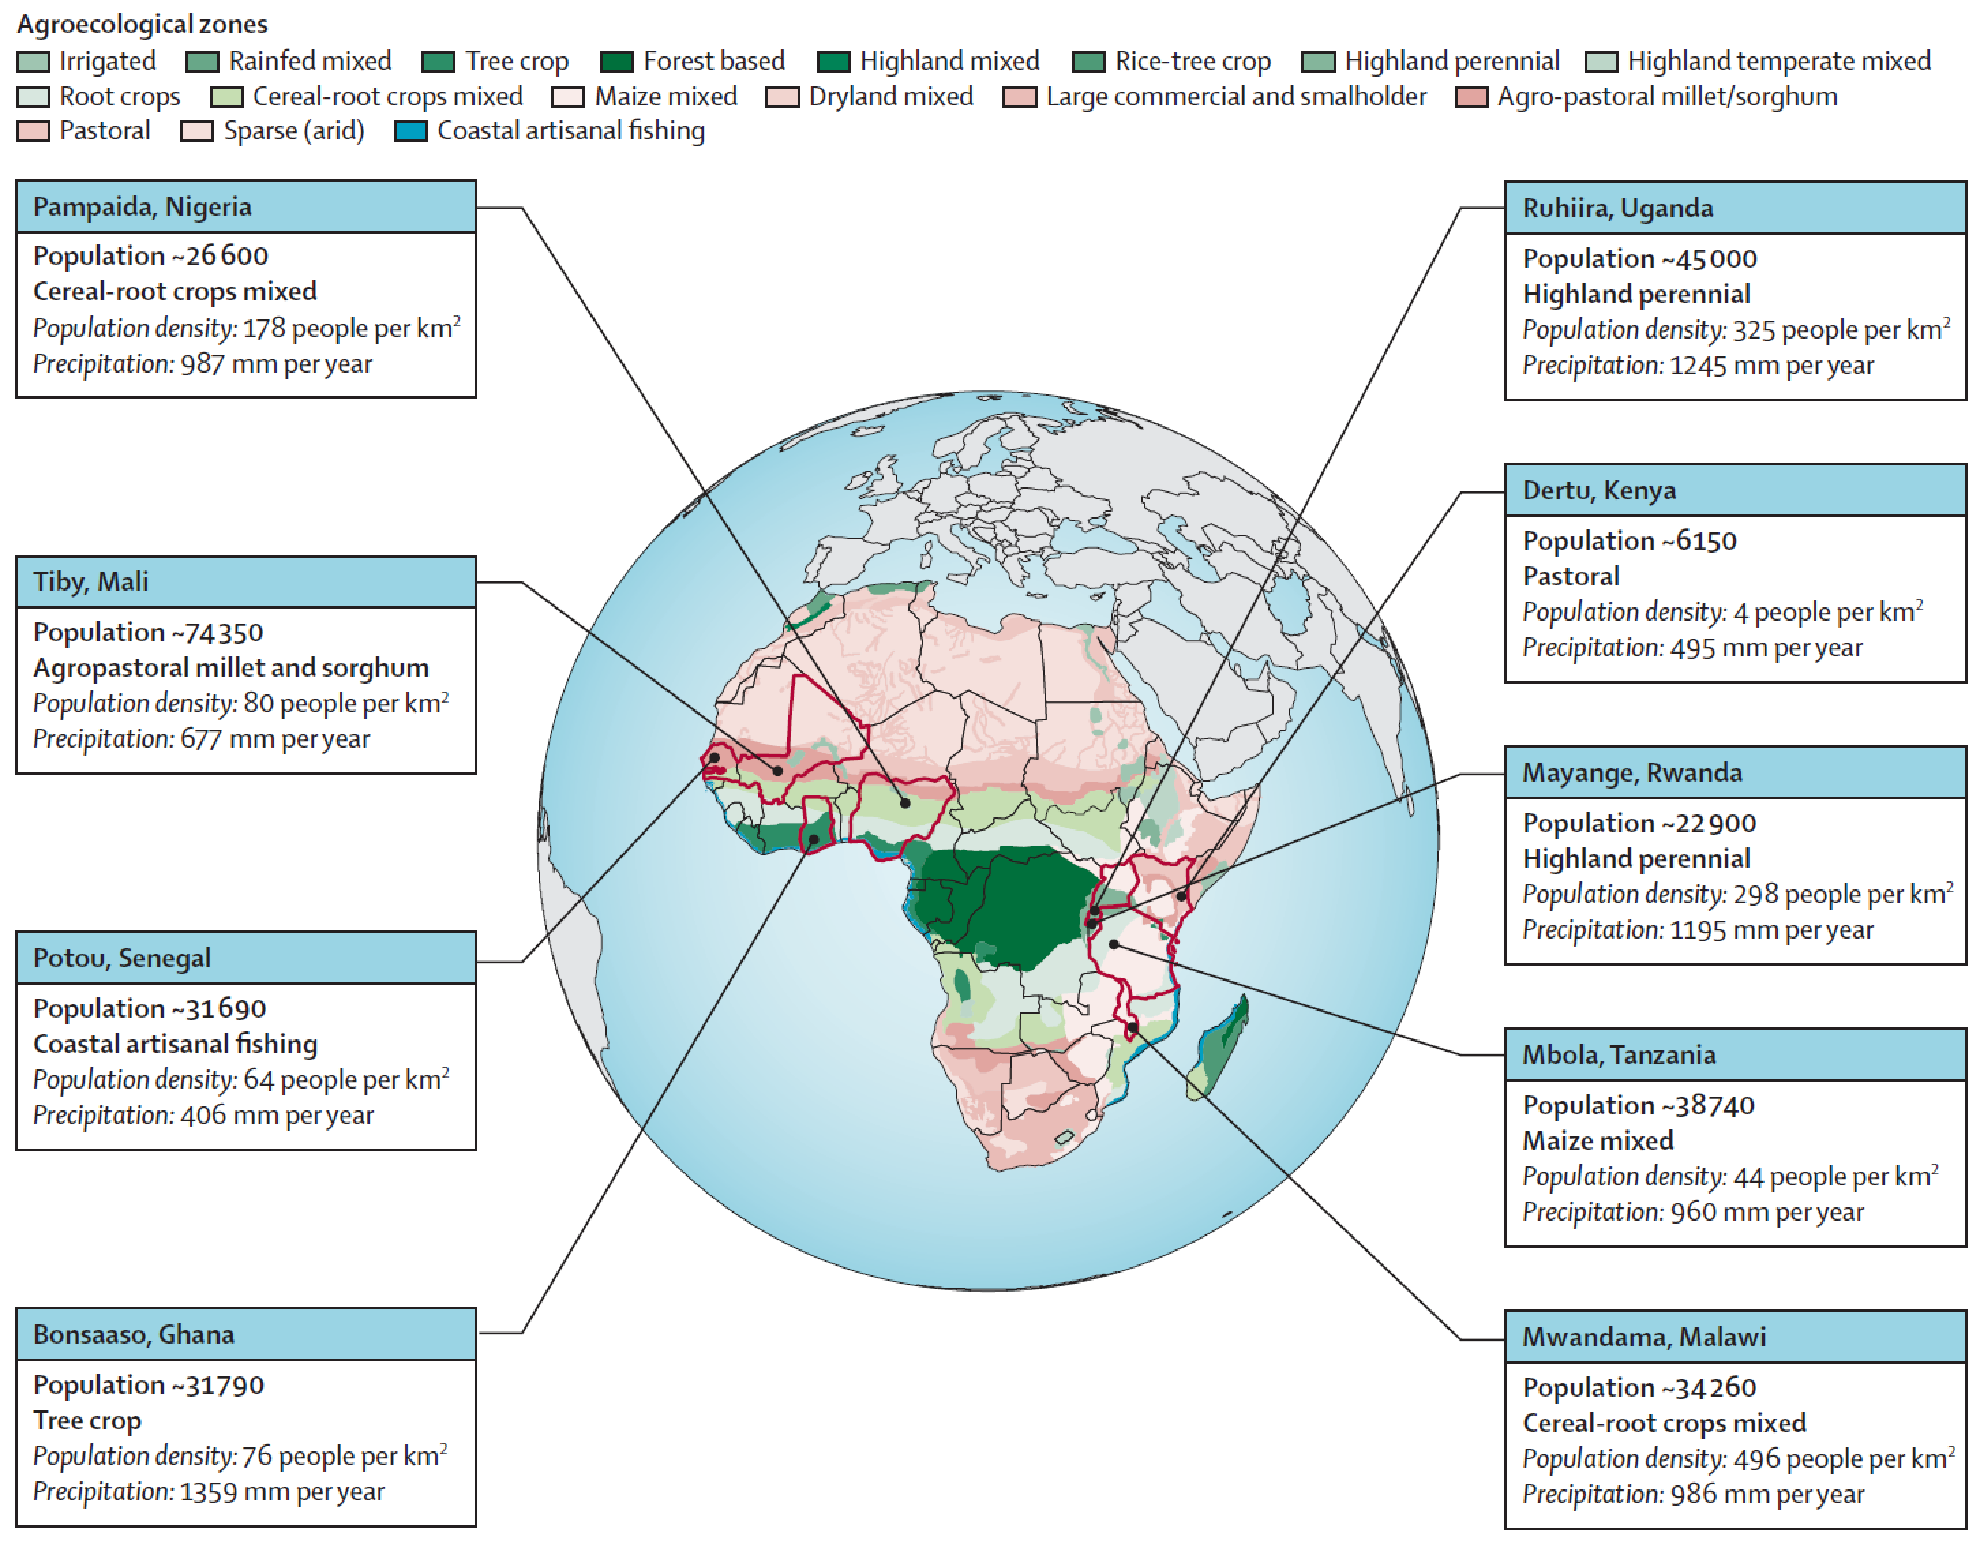
\includegraphics[keepaspectratio,width=7.2cm]{img/MVPmap.pdf}};
	\node [gray,anchor=north] at ([yshift=0.25cm]pronykF1.south)  {\tiny{source:  Pronyk et al.~(2012)}};
	
	\end{tikzpicture}
\end{center}
\end{frame}


%%%%%%%%%%%%%%%%%%%%%%%%%%%%%%%%%%%%%%%%%%%%%%%%%%%%%%%%%%%%%%%%%%%%%%%

\begin{frame}<handout:0>{The Millennium Villages Project}

\begin{center}
	\begin{tikzpicture}
	
	% blank canvas
	\only<handout>{\fill[fill=white,draw=white,ultra thin]
		(0,0) -- (11,0) -- (11,6) -- (0,6) -- cycle;}
	\only<beamer>{\fill[fill=white,draw=white,ultra thin]
		(0,0) -- (14,0) -- (14,6) -- (0,6) -- cycle;}
	\only<beamer>{\draw[draw=oiblue!60,fill=oiblue!10,opacity=0.5] (11,1) rectangle (14,5);}
	%\draw[step=1.0,gray!20,thin] (0,0) grid (11,6);
	
	%	\pgfmathsetmacro\xshift{0.5cm};
	%	\pgfmathsetmacro\yshift{5.5cm};
	%	\pgfmathsetmacro\mycolor{"gray"};
	
	\node [anchor=north] (pronykF1) at (6,6)  {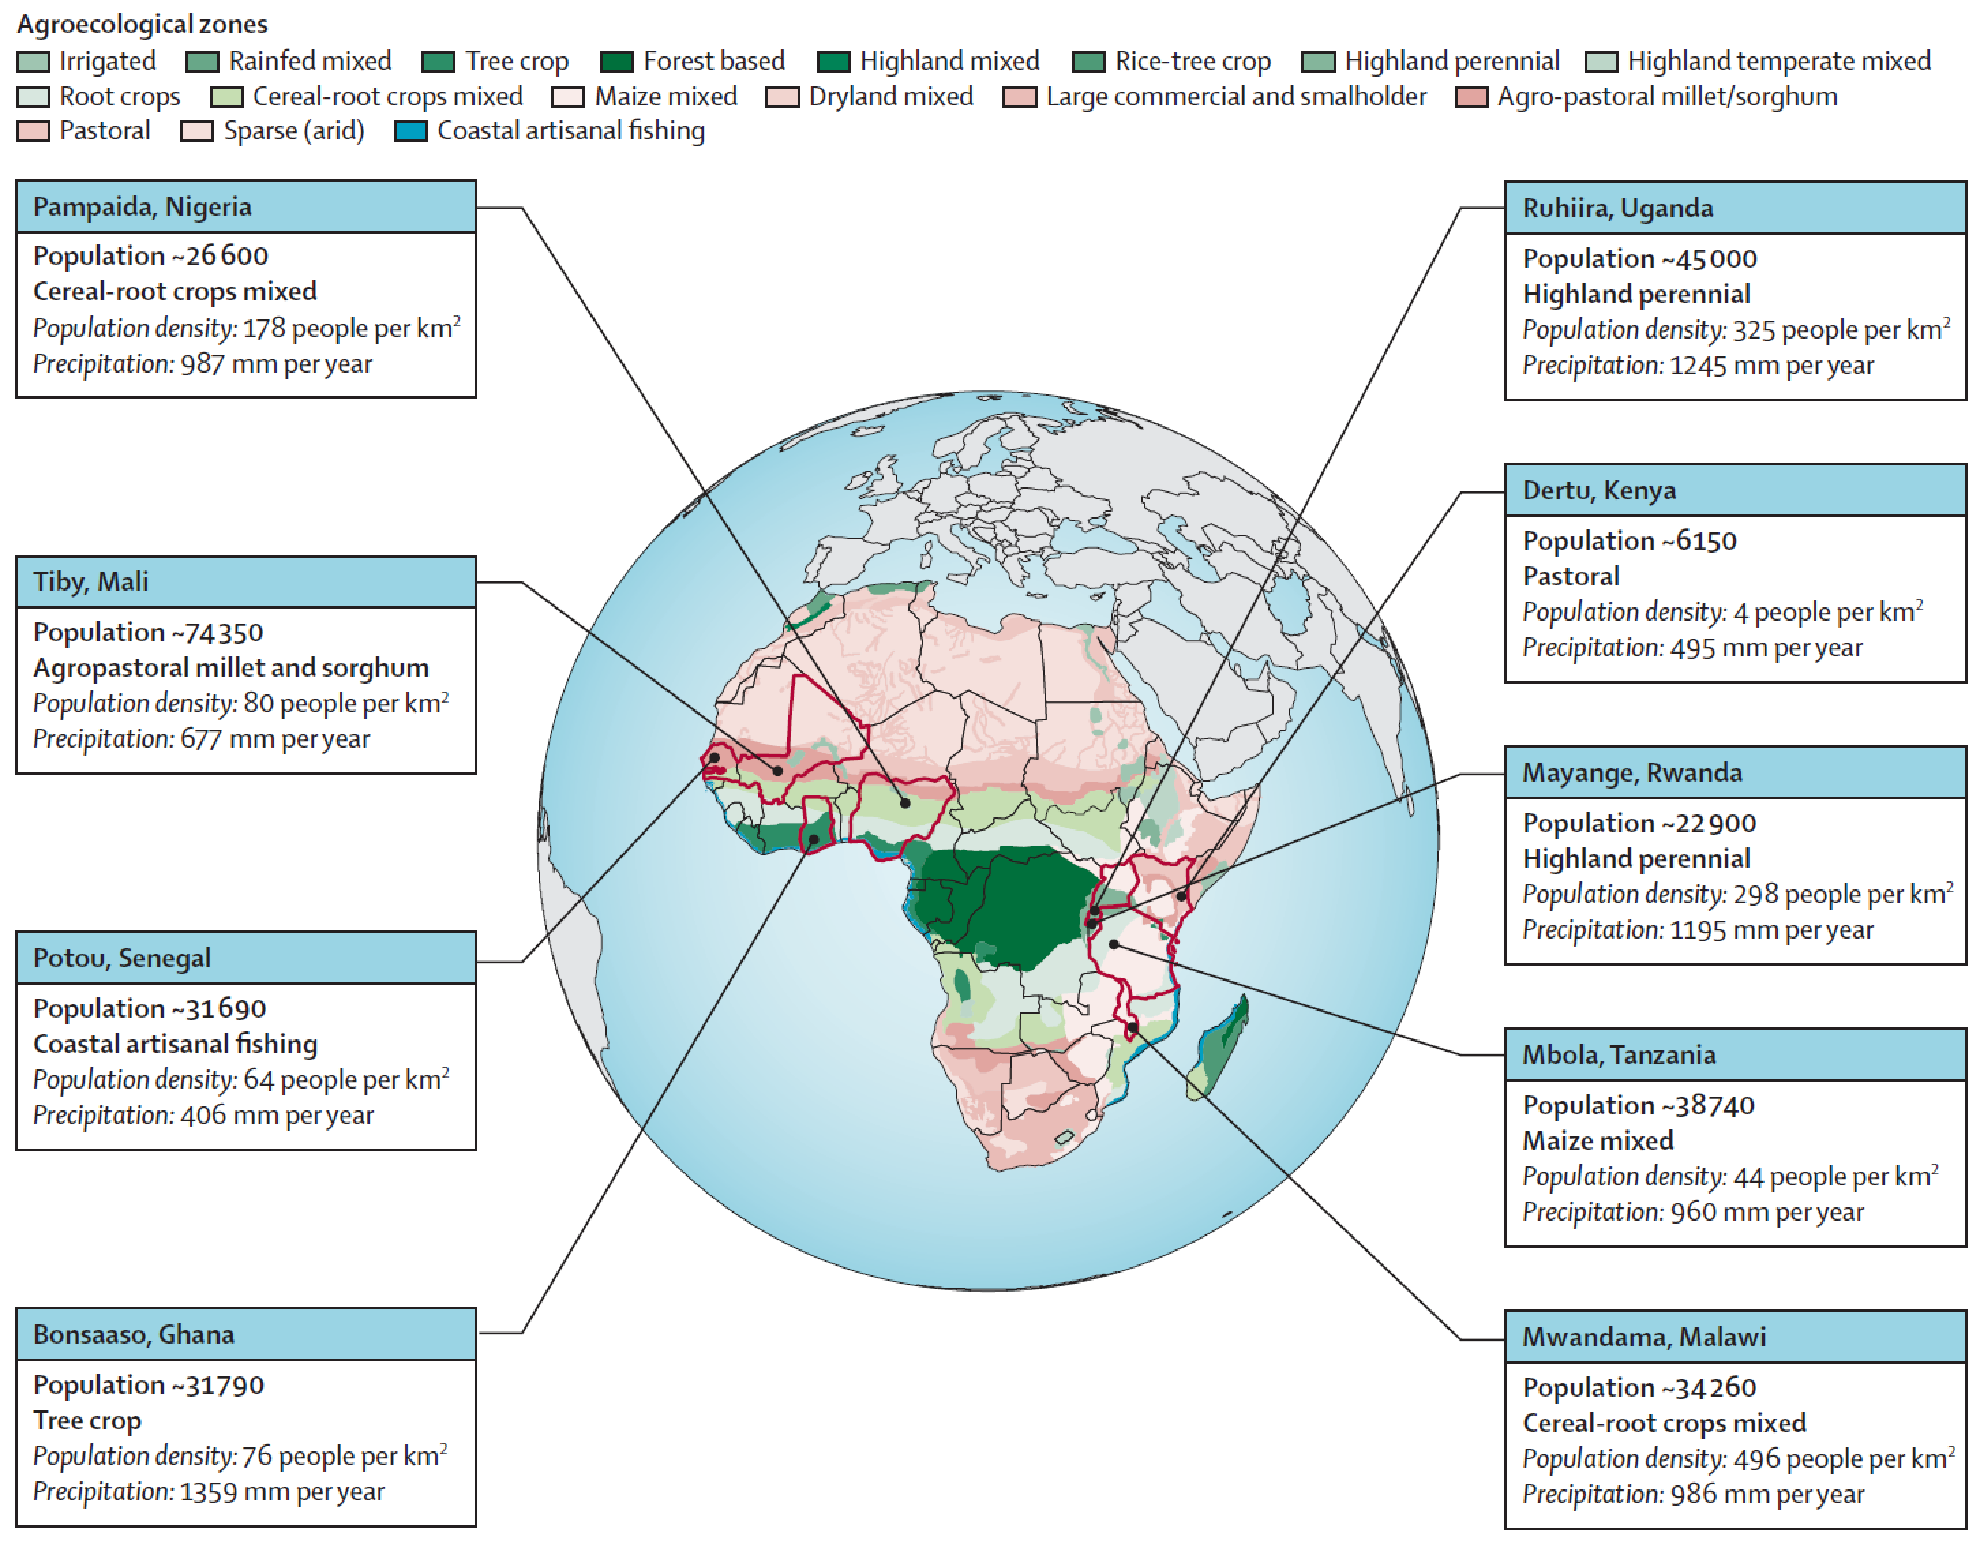
\includegraphics[keepaspectratio,width=7.2cm]{img/MVPmap.pdf}};
	\node [gray,anchor=north] at ([yshift=0.25cm]pronykF1.south)  {\tiny{source:  Pronyk et al.~(2012)}};

	\node [anchor=north] (sachs) at (1.25,6)  {
\includegraphics[keepaspectratio,width=2cm]{photos/sachs-rick-bajornas.jpg}};
	\node [gray,anchor=north] at ([yshift=0.125cm]sachs.south)  {\tiny{photo:  Rick Bajornas}};
	
	\end{tikzpicture}
\end{center}
\end{frame}



%%%%%%%%%%%%%%%%%%%%%%%%%%%%%%%%%%%%%%%%%%%%%%%%%%%%%%%%%%%%%%%%%%%%%%%

\begin{frame}<handout:0>{The Millennium Villages Project:  A Big Push}

\begin{center}
	\begin{tikzpicture}
	
	% blank canvas
	\only<handout>{\fill[fill=white,draw=white,ultra thin]
		(0,0) -- (11,0) -- (11,6) -- (0,6) -- cycle;}
	\only<beamer>{\fill[fill=white,draw=white,ultra thin]
		(0,0) -- (14,0) -- (14,6) -- (0,6) -- cycle;}
	\only<beamer>{\draw[draw=oiblue!60,fill=oiblue!10,opacity=0.5] (11,1) rectangle (14,5);}
	%\draw[step=1.0,gray!20,thin] (0,0) grid (11,6);
	
	%	\pgfmathsetmacro\xshift{0.5cm};
	%	\pgfmathsetmacro\yshift{5.5cm};
	%	\pgfmathsetmacro\mycolor{"gray"};
	
	\node [anchor=north] (pronykF1) at (6,6)  {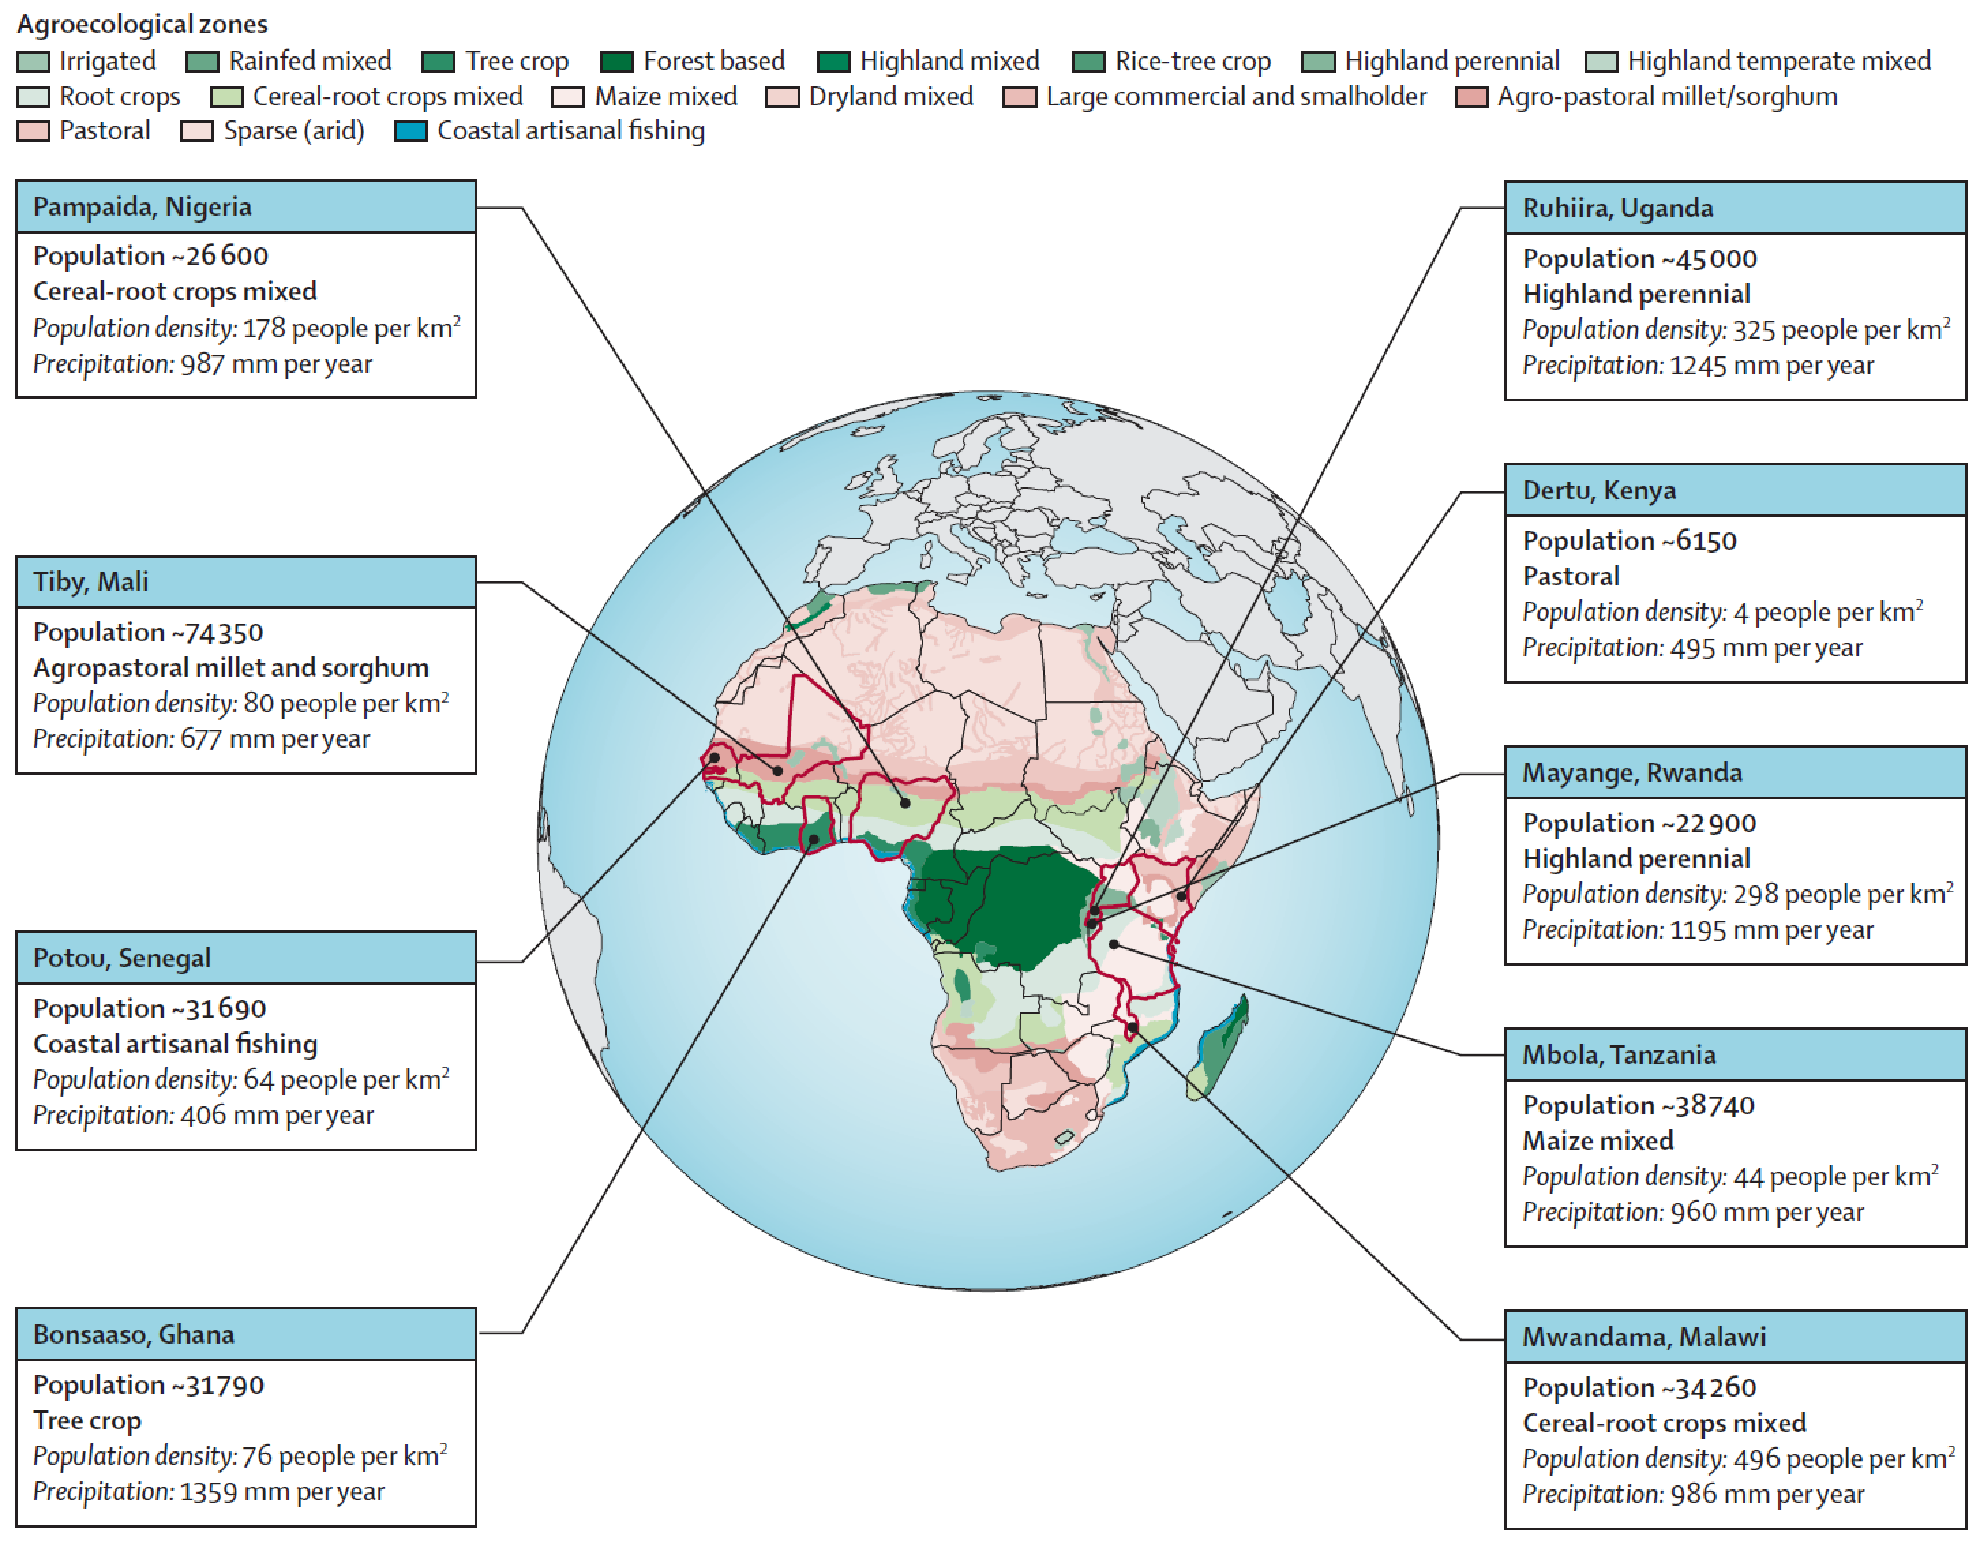
\includegraphics[keepaspectratio,width=7.2cm]{img/MVPmap.pdf}};
	\node [gray,anchor=north] at ([yshift=0.25cm]pronykF1.south)  {\tiny{source:  Pronyk et al.~(2012)}};

	\node [anchor=north] (sachs) at (1.25,6)  {
\includegraphics[keepaspectratio,width=2cm]{photos/sachs-rick-bajornas.jpg}};
	\node [gray,anchor=north] at ([yshift=0.125cm]sachs.south)  {\tiny{photo:  Rick Bajornas}};
	\node [anchor=north] (school) at (1.25,4.375)  {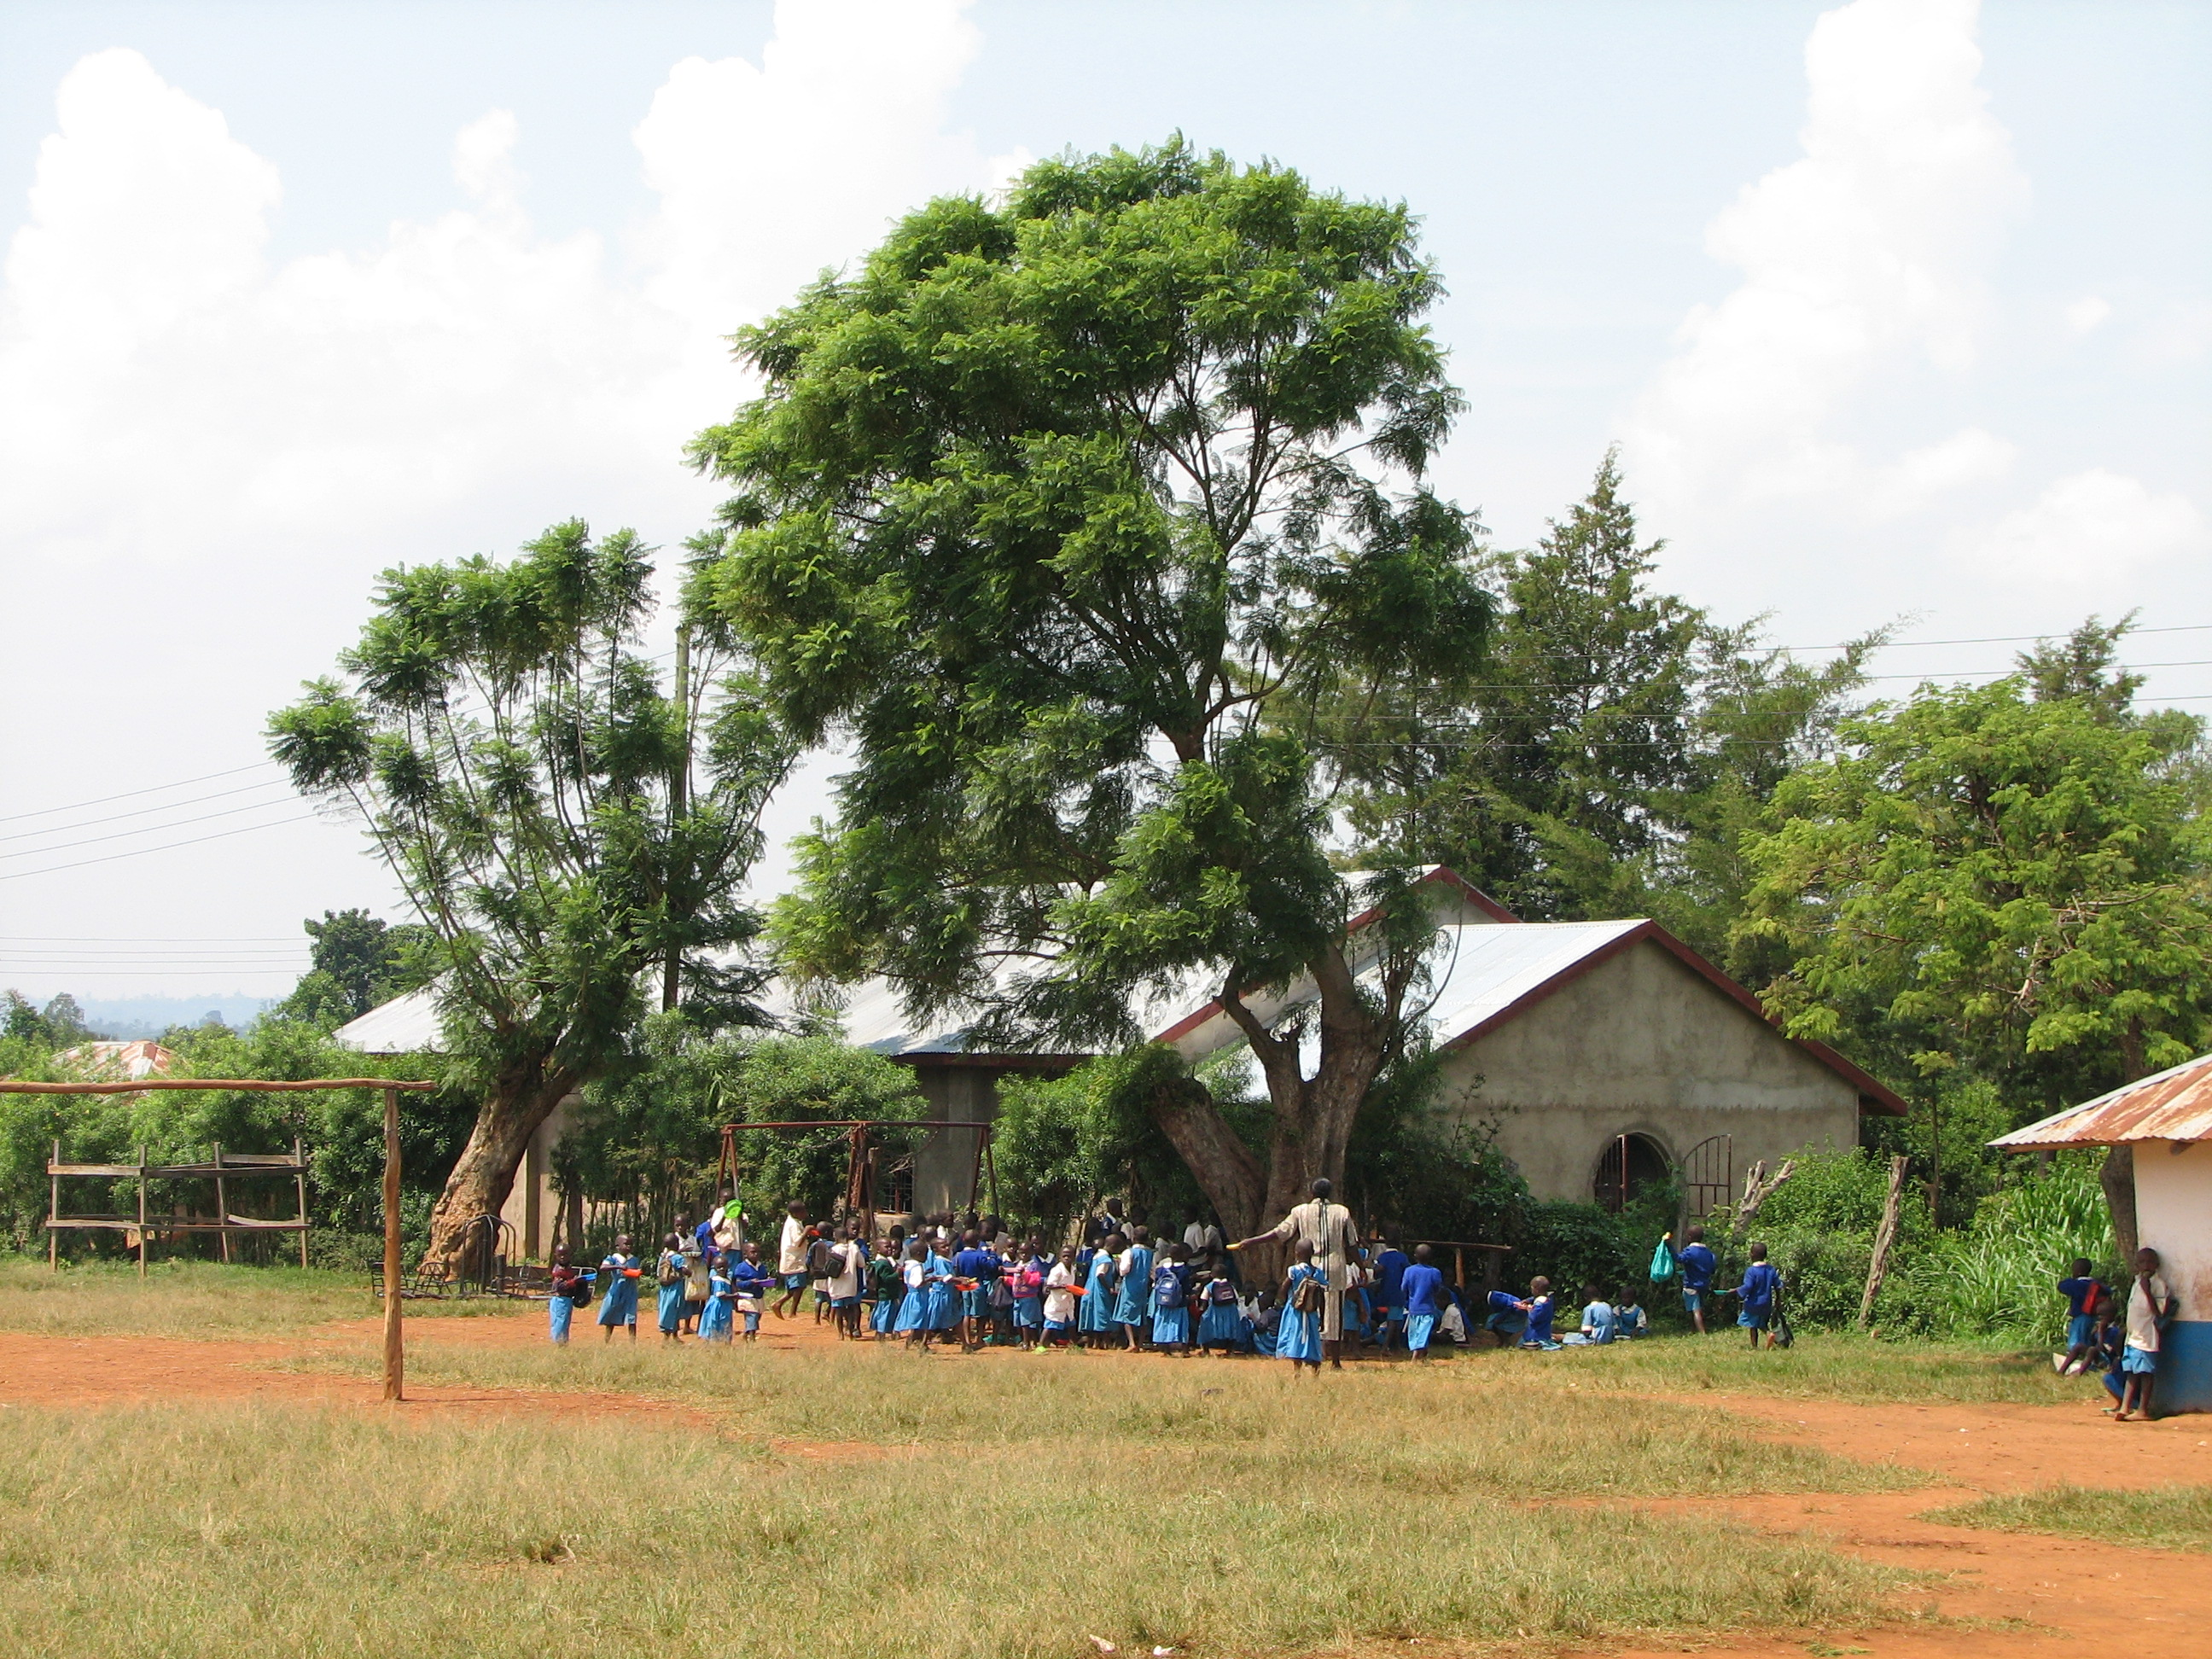
\includegraphics[keepaspectratio,width=1.6cm]{photos/sauri-primary.jpg}};
	\node [yellow,anchor=south west,align=left] at ([xshift=0.05cm,yshift=0.05cm]school.south west)  {\tiny{schools}};
	%\node [anchor=north] (crops) at (1.25,3)  {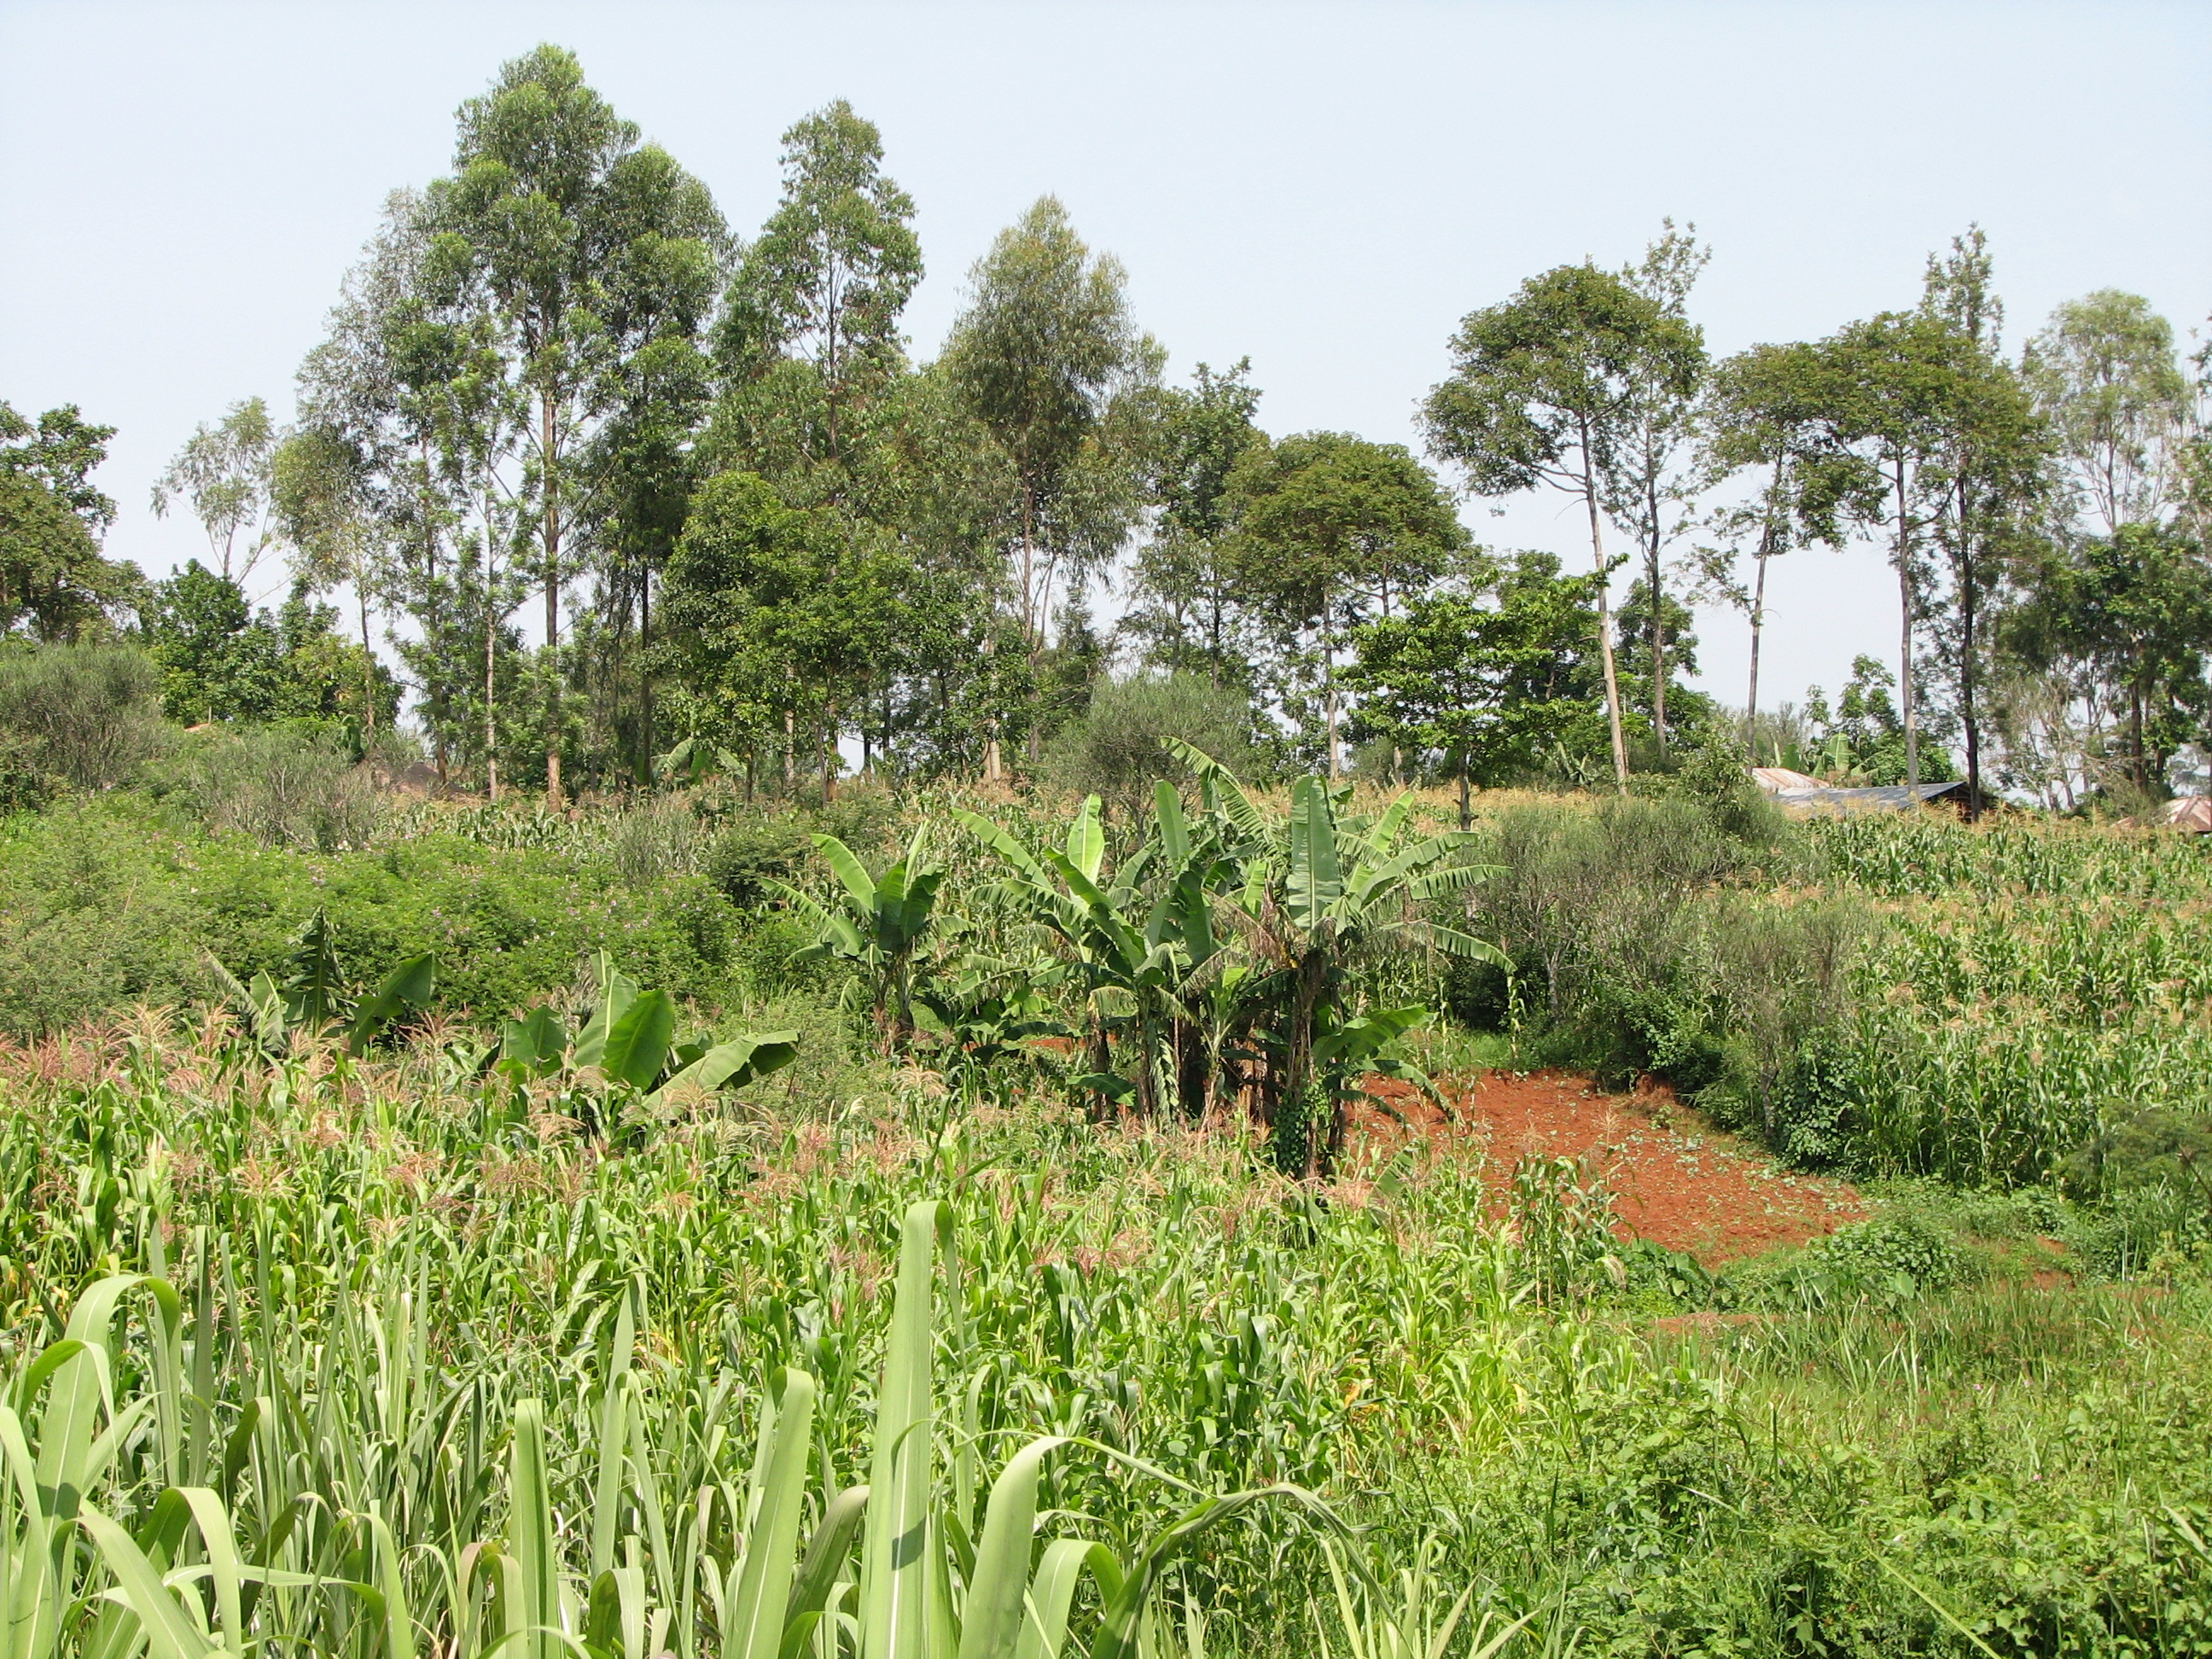
\includegraphics[keepaspectratio,width=1.6cm]{photos/sauri-crops.jpg}};
	%\node [yellow,anchor=south west,align=left] at ([xshift=0.05cm,yshift=0.05cm]crops.south west)  {\tiny{agriculture}};
	%\node [anchor=north] (health) at (1.25,1.625)  {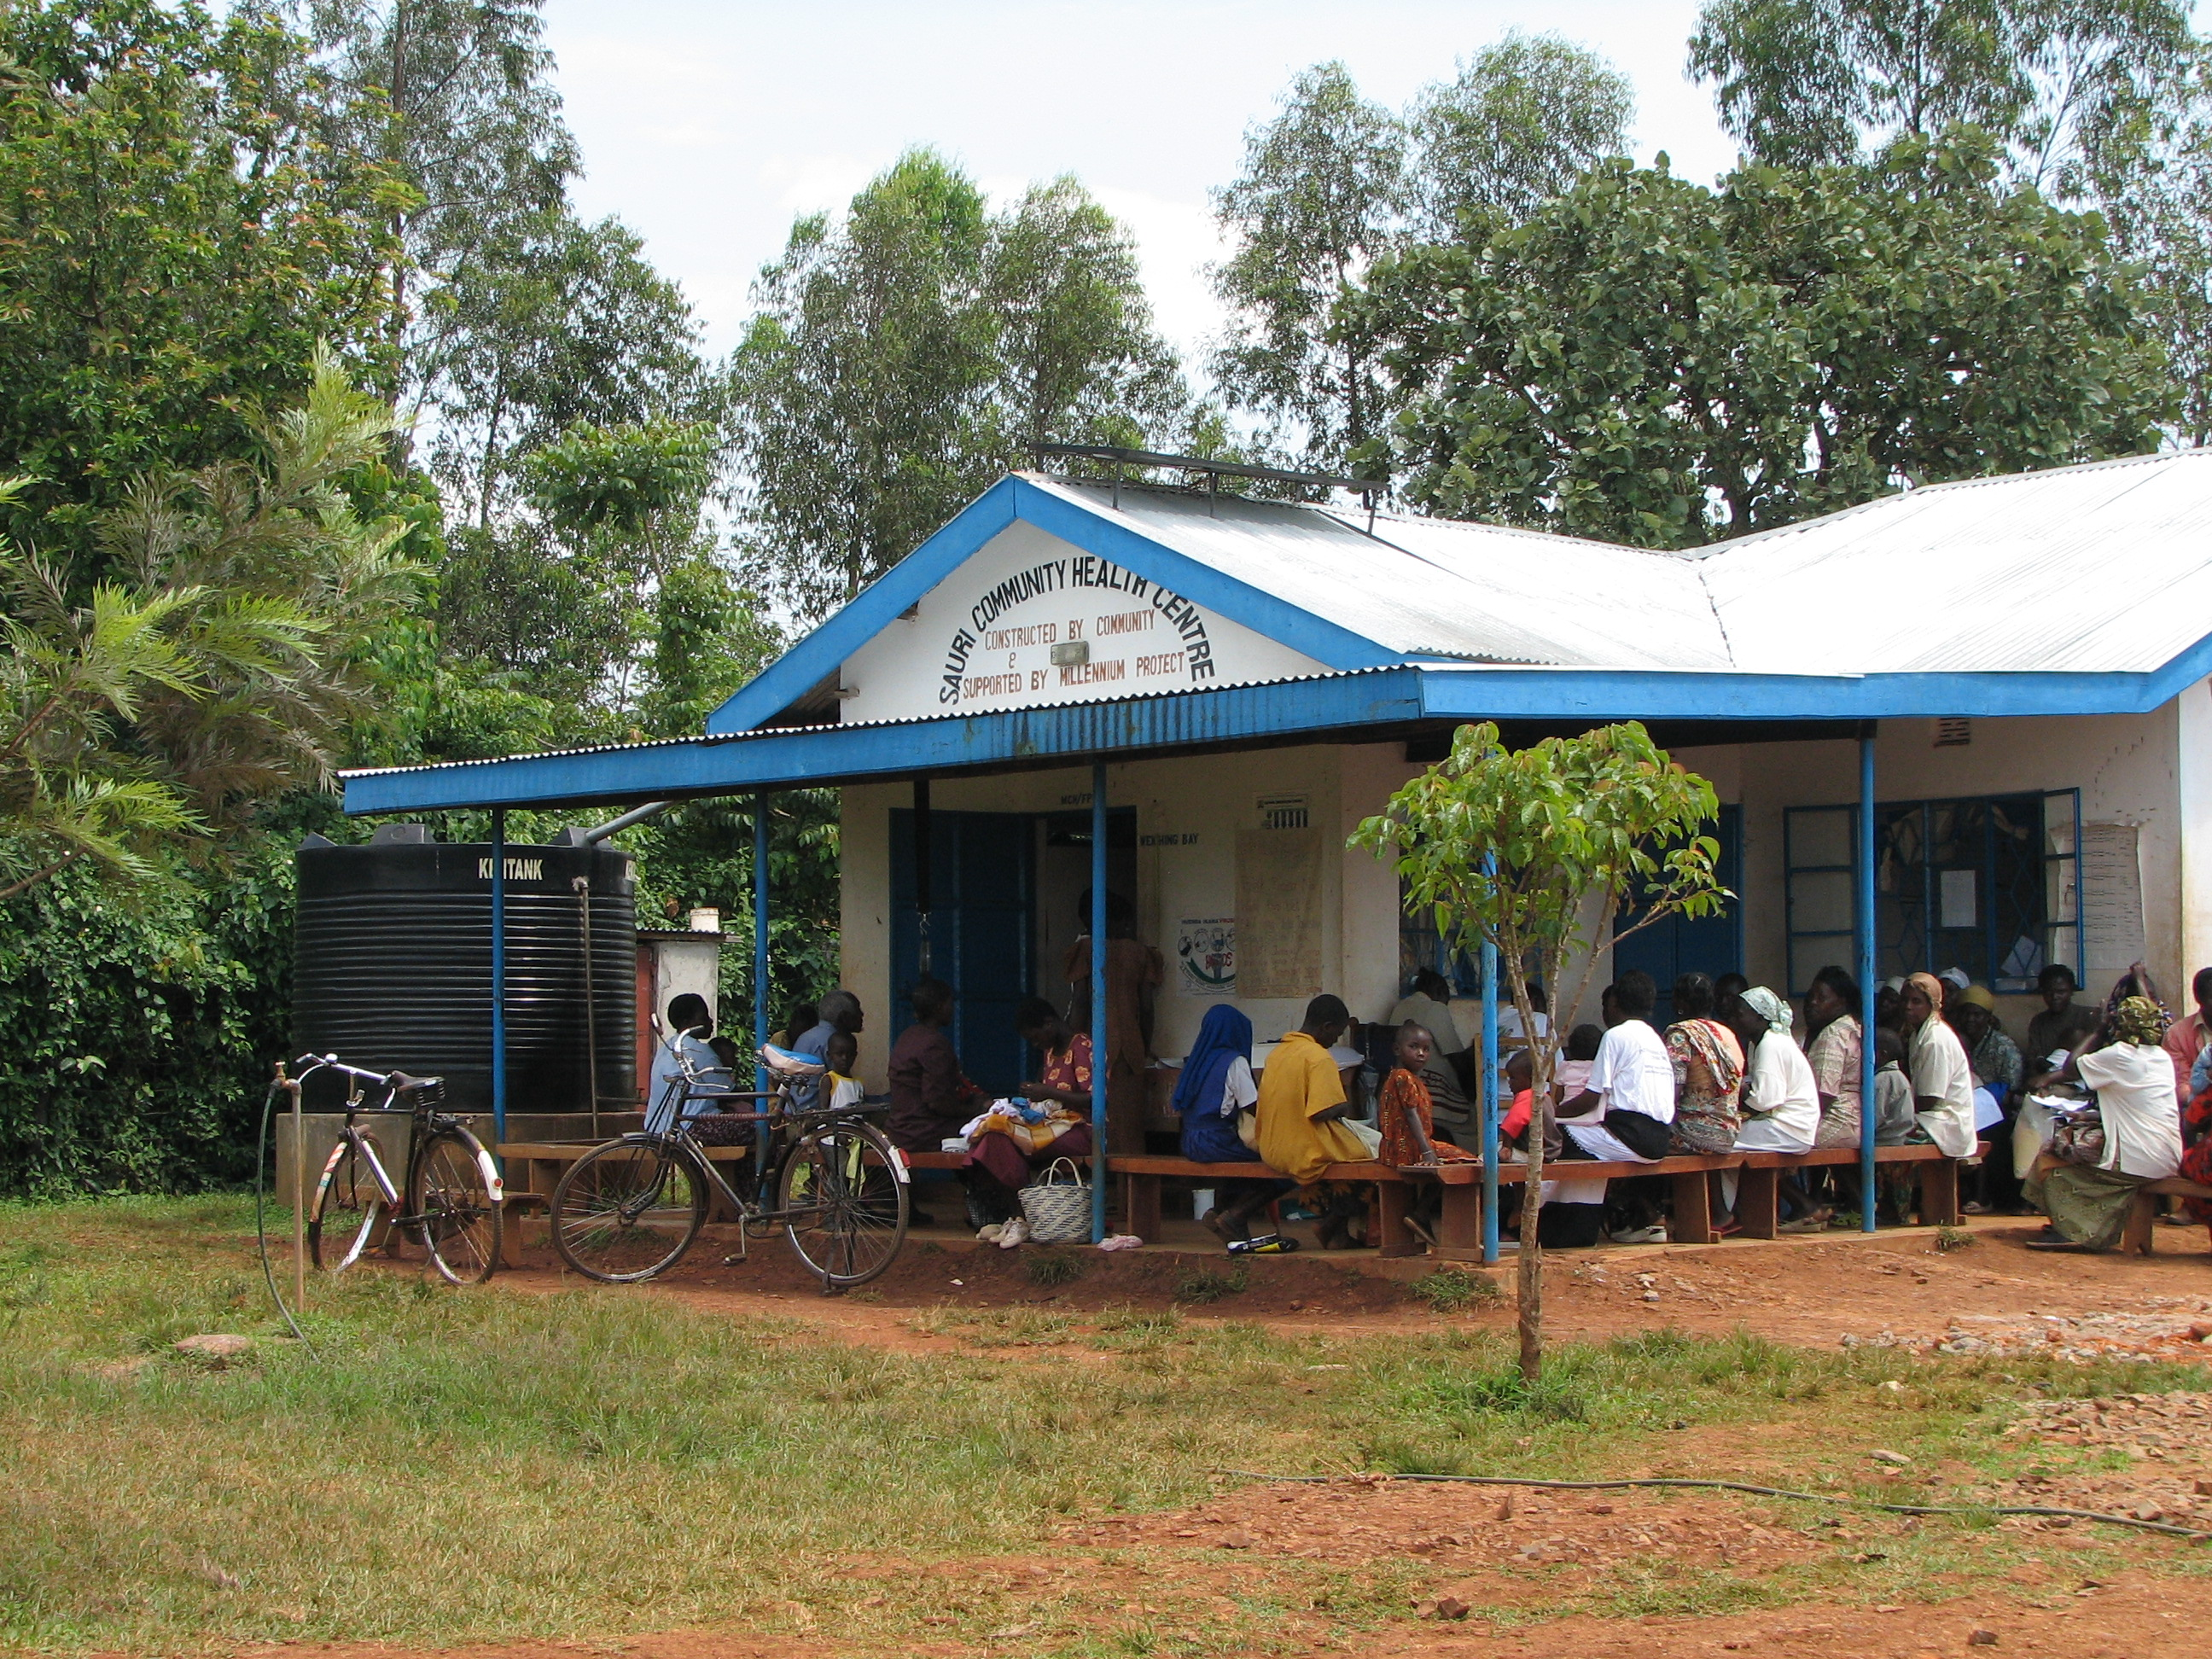
\includegraphics[keepaspectratio,width=1.6cm]{photos/sauri-health-center.jpg}};
	%\node [yellow,anchor=south west,align=left] at ([xshift=0.05cm,yshift=0.05cm]health.south west)  {\tiny{health}};
	
	\end{tikzpicture}
\end{center}
\end{frame}


%%%%%%%%%%%%%%%%%%%%%%%%%%%%%%%%%%%%%%%%%%%%%%%%%%%%%%%%%%%%%%%%%%%%%%%

\begin{frame}<handout:0>{The Millennium Villages Project:  A Big Push}

\begin{center}
	\begin{tikzpicture}
	
	% blank canvas
	\only<handout>{\fill[fill=white,draw=white,ultra thin]
		(0,0) -- (11,0) -- (11,6) -- (0,6) -- cycle;}
	\only<beamer>{\fill[fill=white,draw=white,ultra thin]
		(0,0) -- (14,0) -- (14,6) -- (0,6) -- cycle;}
	\only<beamer>{\draw[draw=oiblue!60,fill=oiblue!10,opacity=0.5] (11,1) rectangle (14,5);}
	%\draw[step=1.0,gray!20,thin] (0,0) grid (11,6);
	
	%	\pgfmathsetmacro\xshift{0.5cm};
	%	\pgfmathsetmacro\yshift{5.5cm};
	%	\pgfmathsetmacro\mycolor{"gray"};
	
	\node [anchor=north] (pronykF1) at (6,6)  {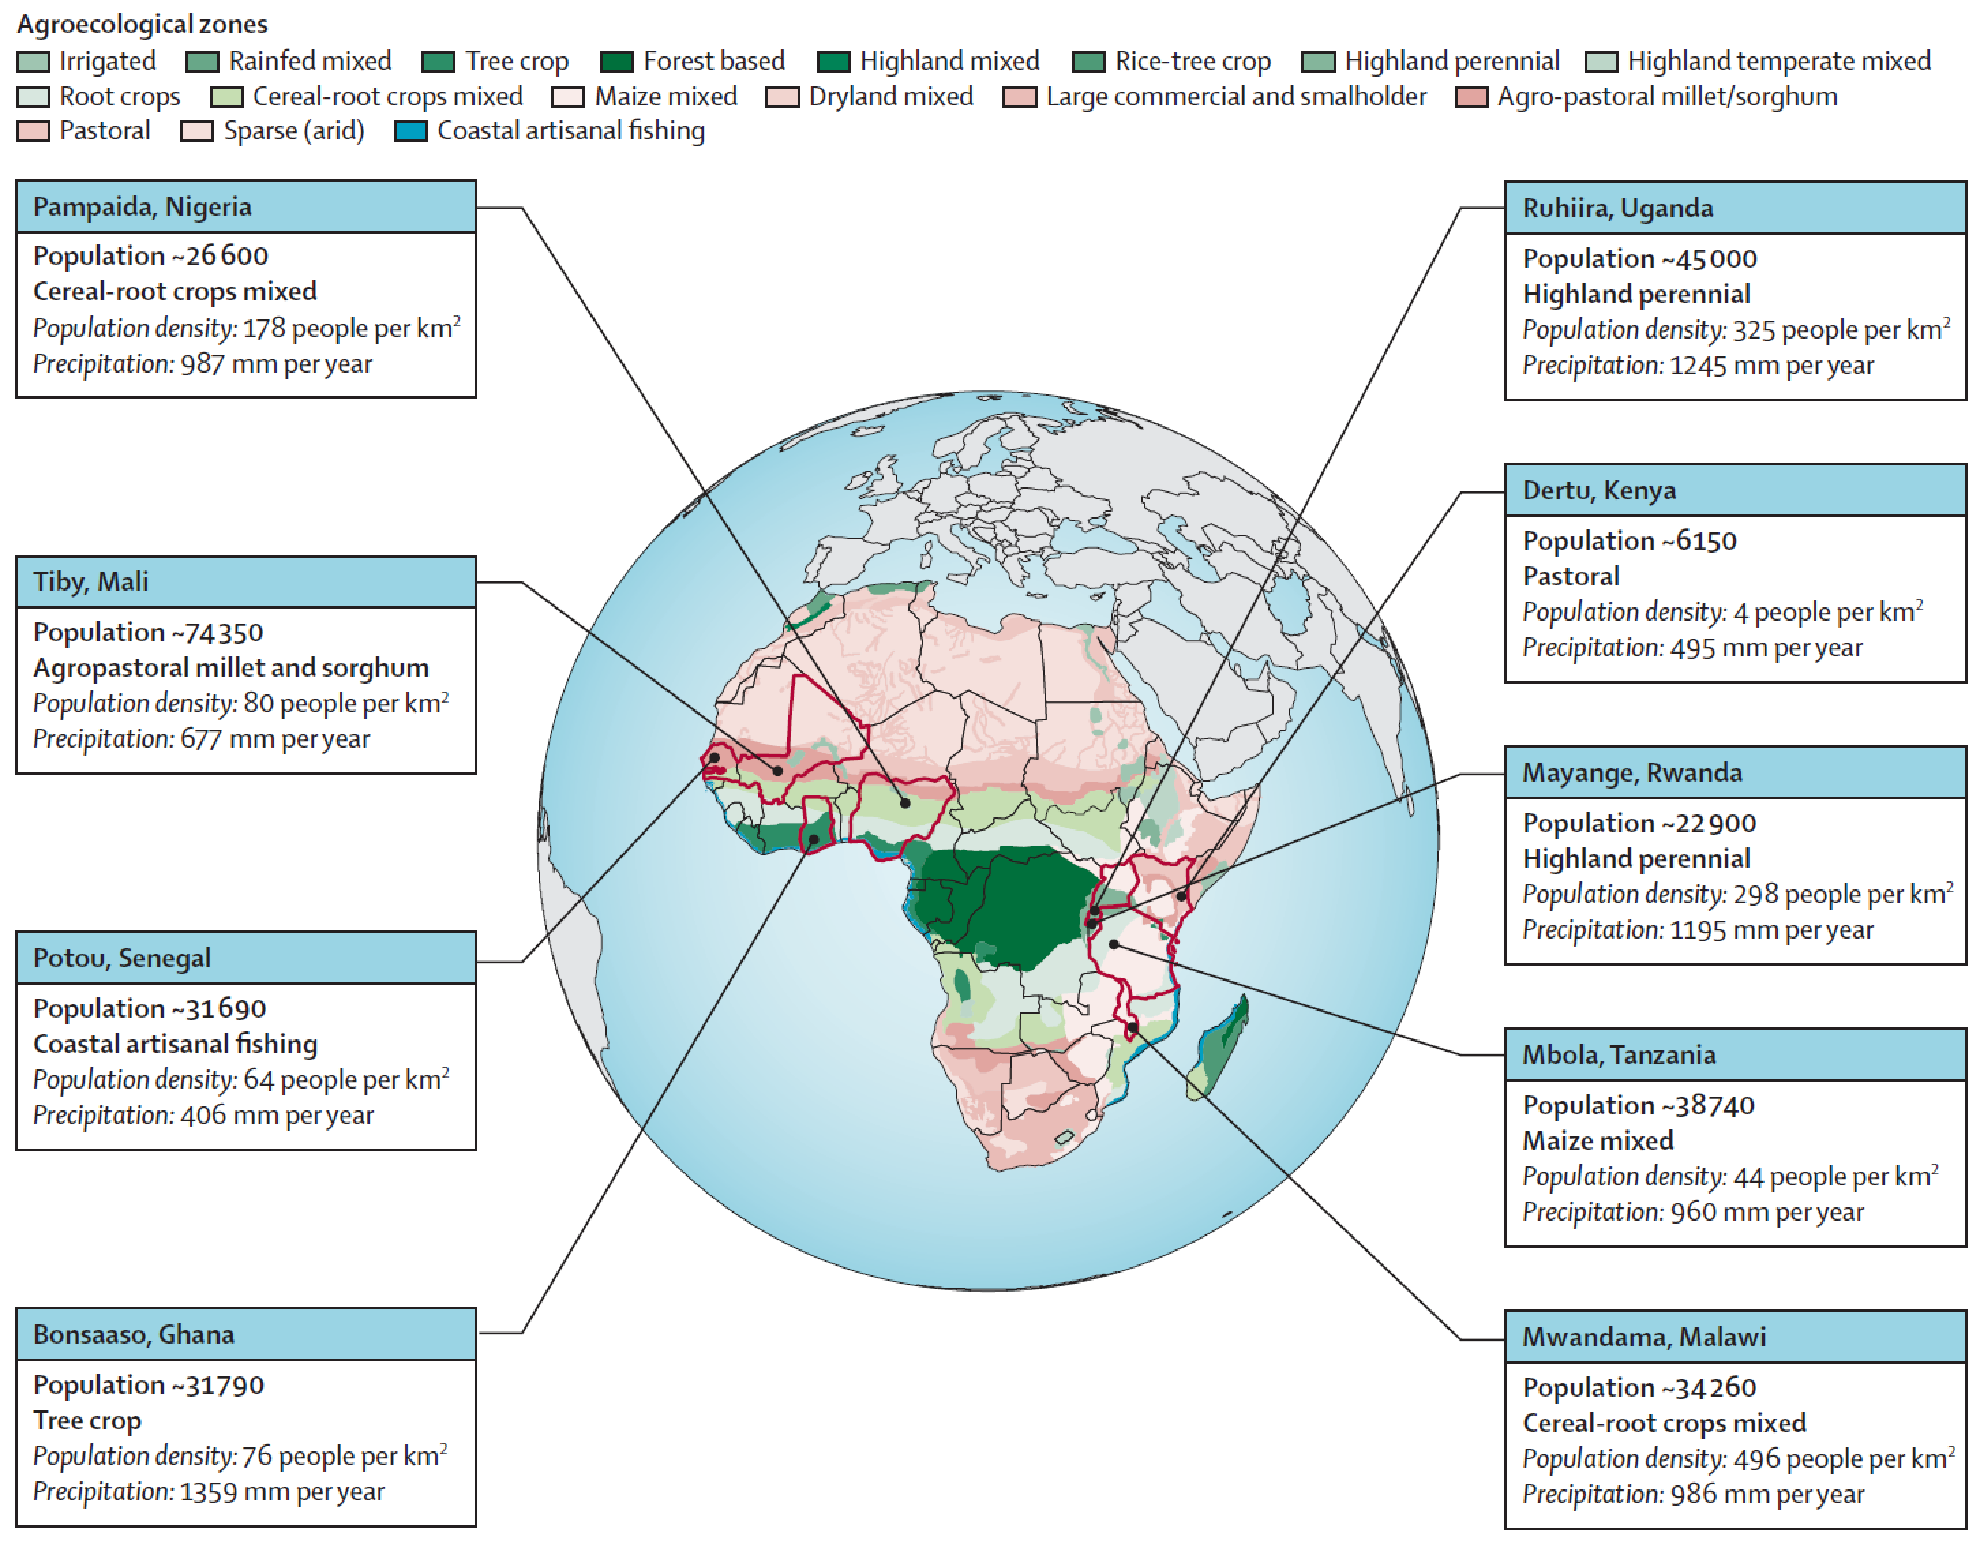
\includegraphics[keepaspectratio,width=7.2cm]{img/MVPmap.pdf}};
	\node [gray,anchor=north] at ([yshift=0.25cm]pronykF1.south)  {\tiny{source:  Pronyk et al.~(2012)}};

	\node [anchor=north] (sachs) at (1.25,6)  {
\includegraphics[keepaspectratio,width=2cm]{photos/sachs-rick-bajornas.jpg}};
	\node [gray,anchor=north] at ([yshift=0.125cm]sachs.south)  {\tiny{photo:  Rick Bajornas}};
	\node [anchor=north] (school) at (1.25,4.375)  {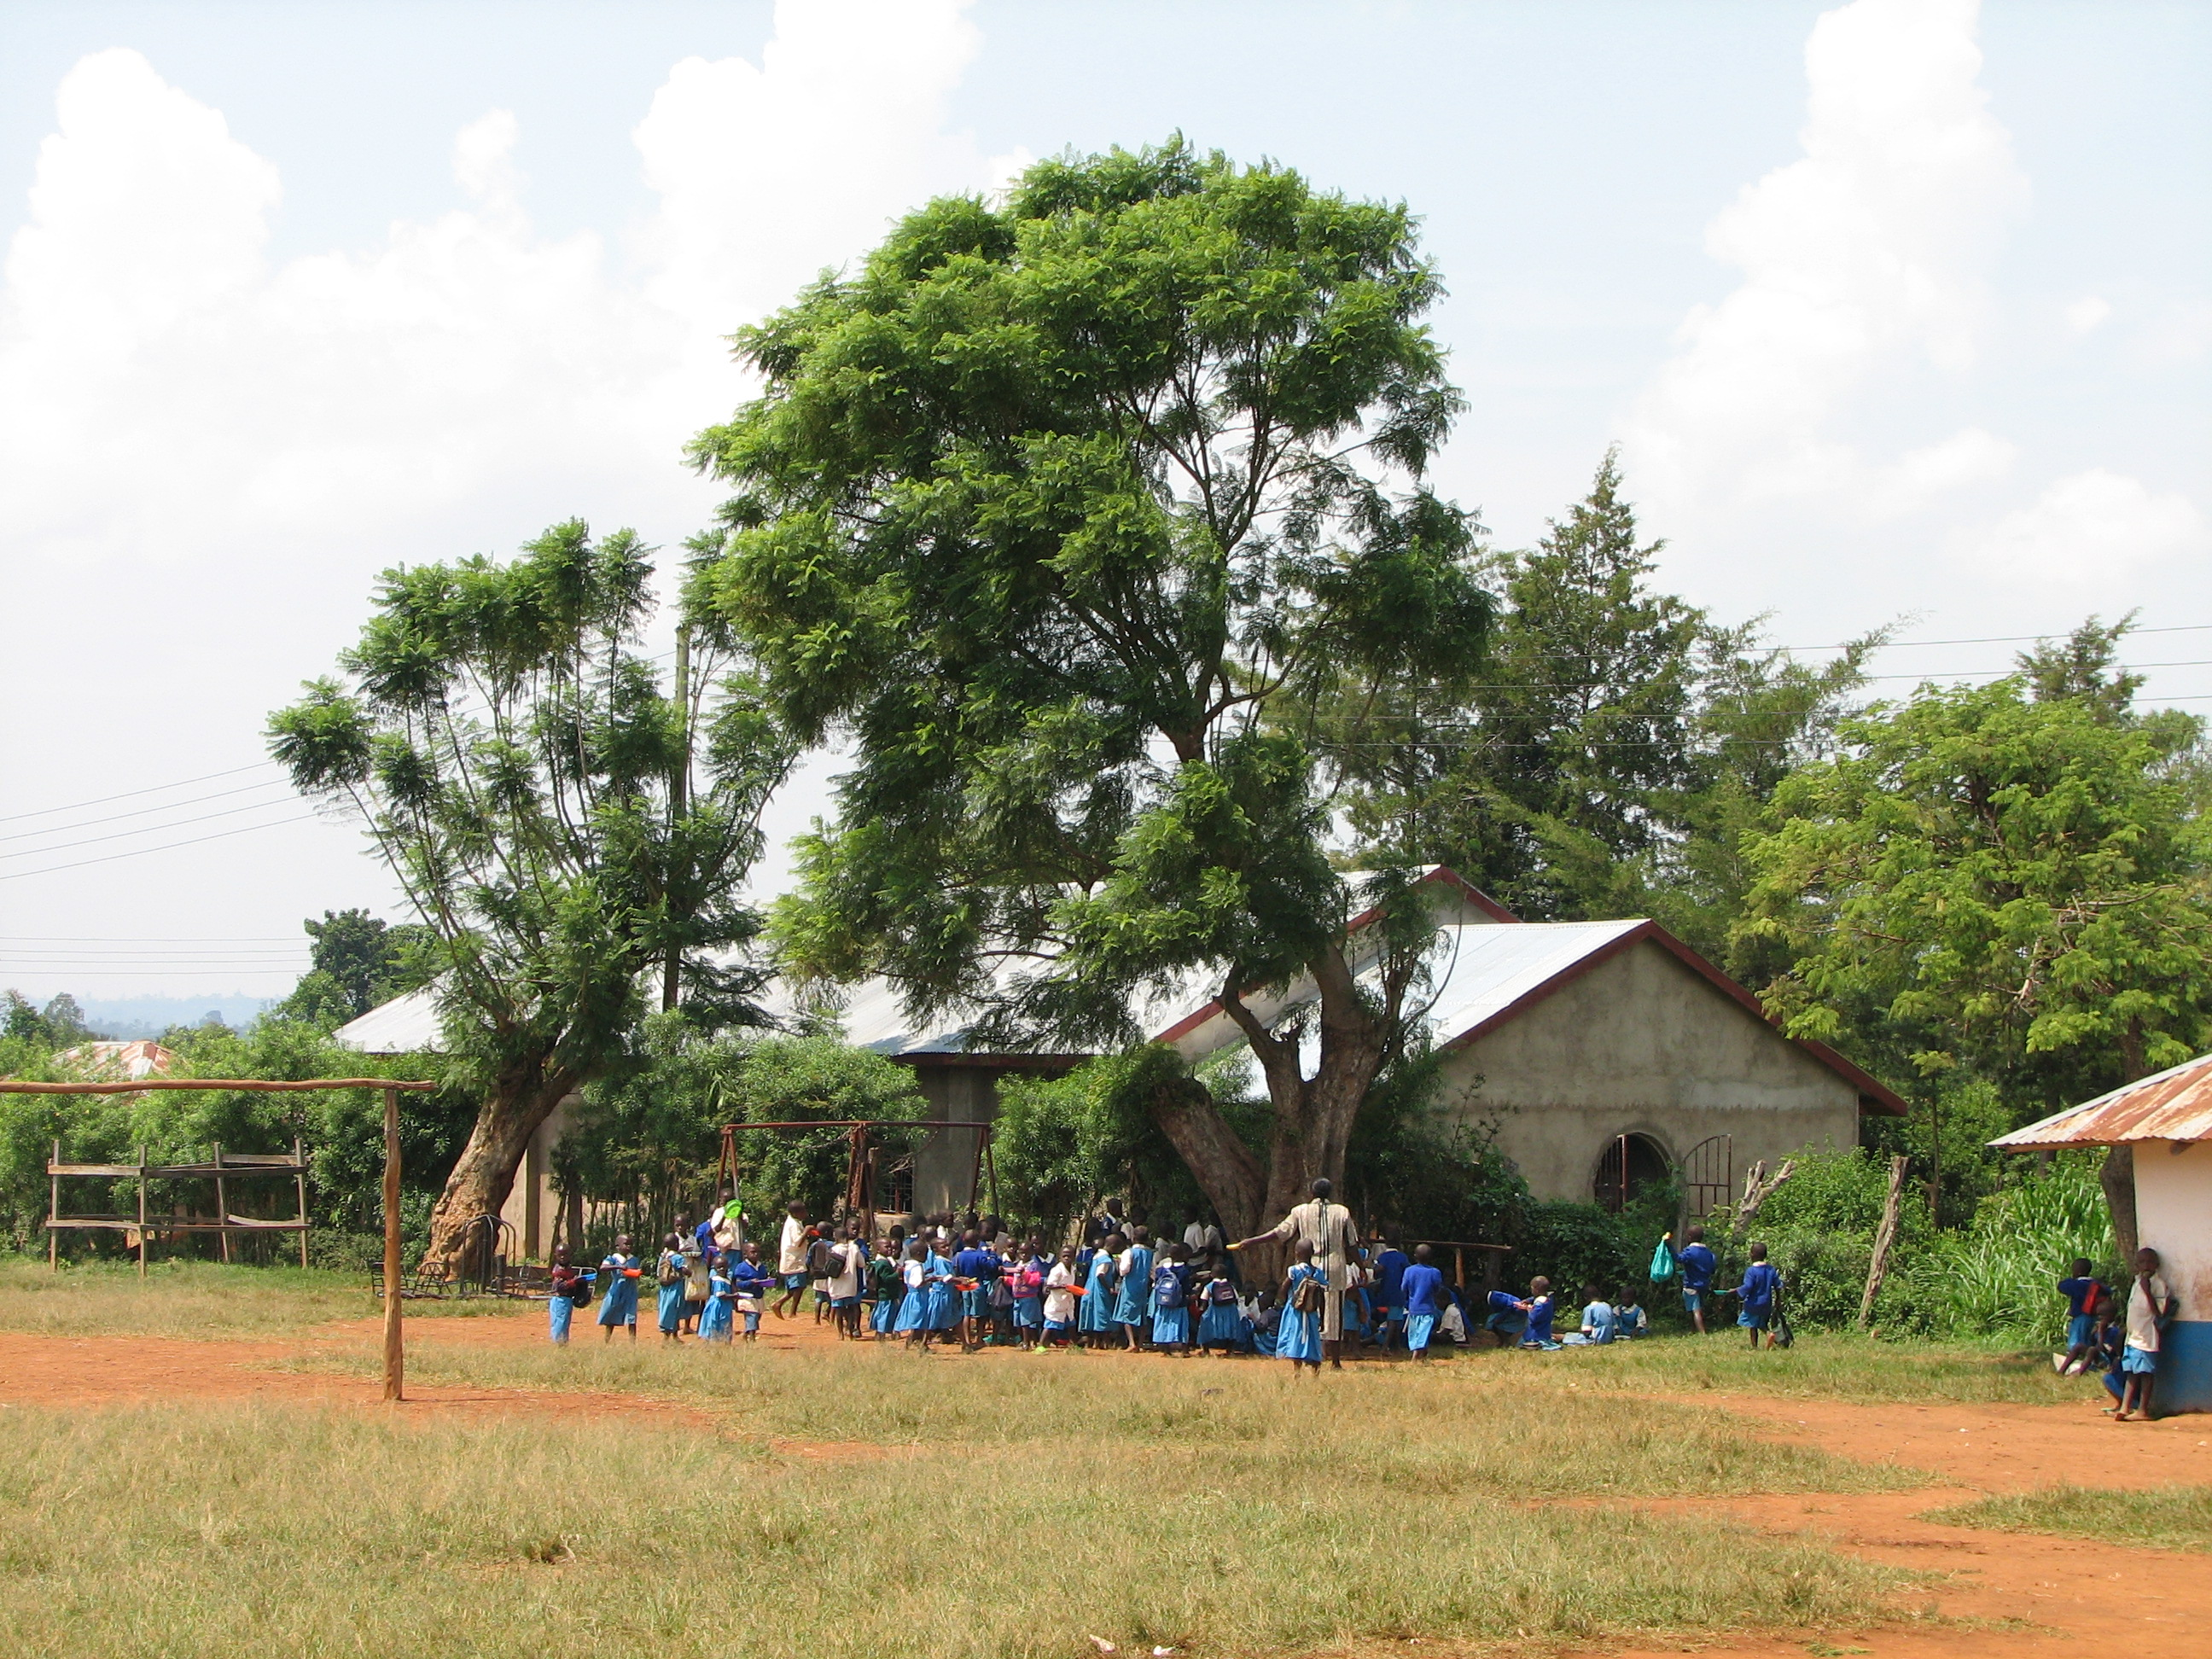
\includegraphics[keepaspectratio,width=1.6cm]{photos/sauri-primary.jpg}};
	\node [yellow,anchor=south west,align=left] at ([xshift=0.05cm,yshift=0.05cm]school.south west)  {\tiny{schools}};
	\node [anchor=north] (crops) at (1.25,3)  {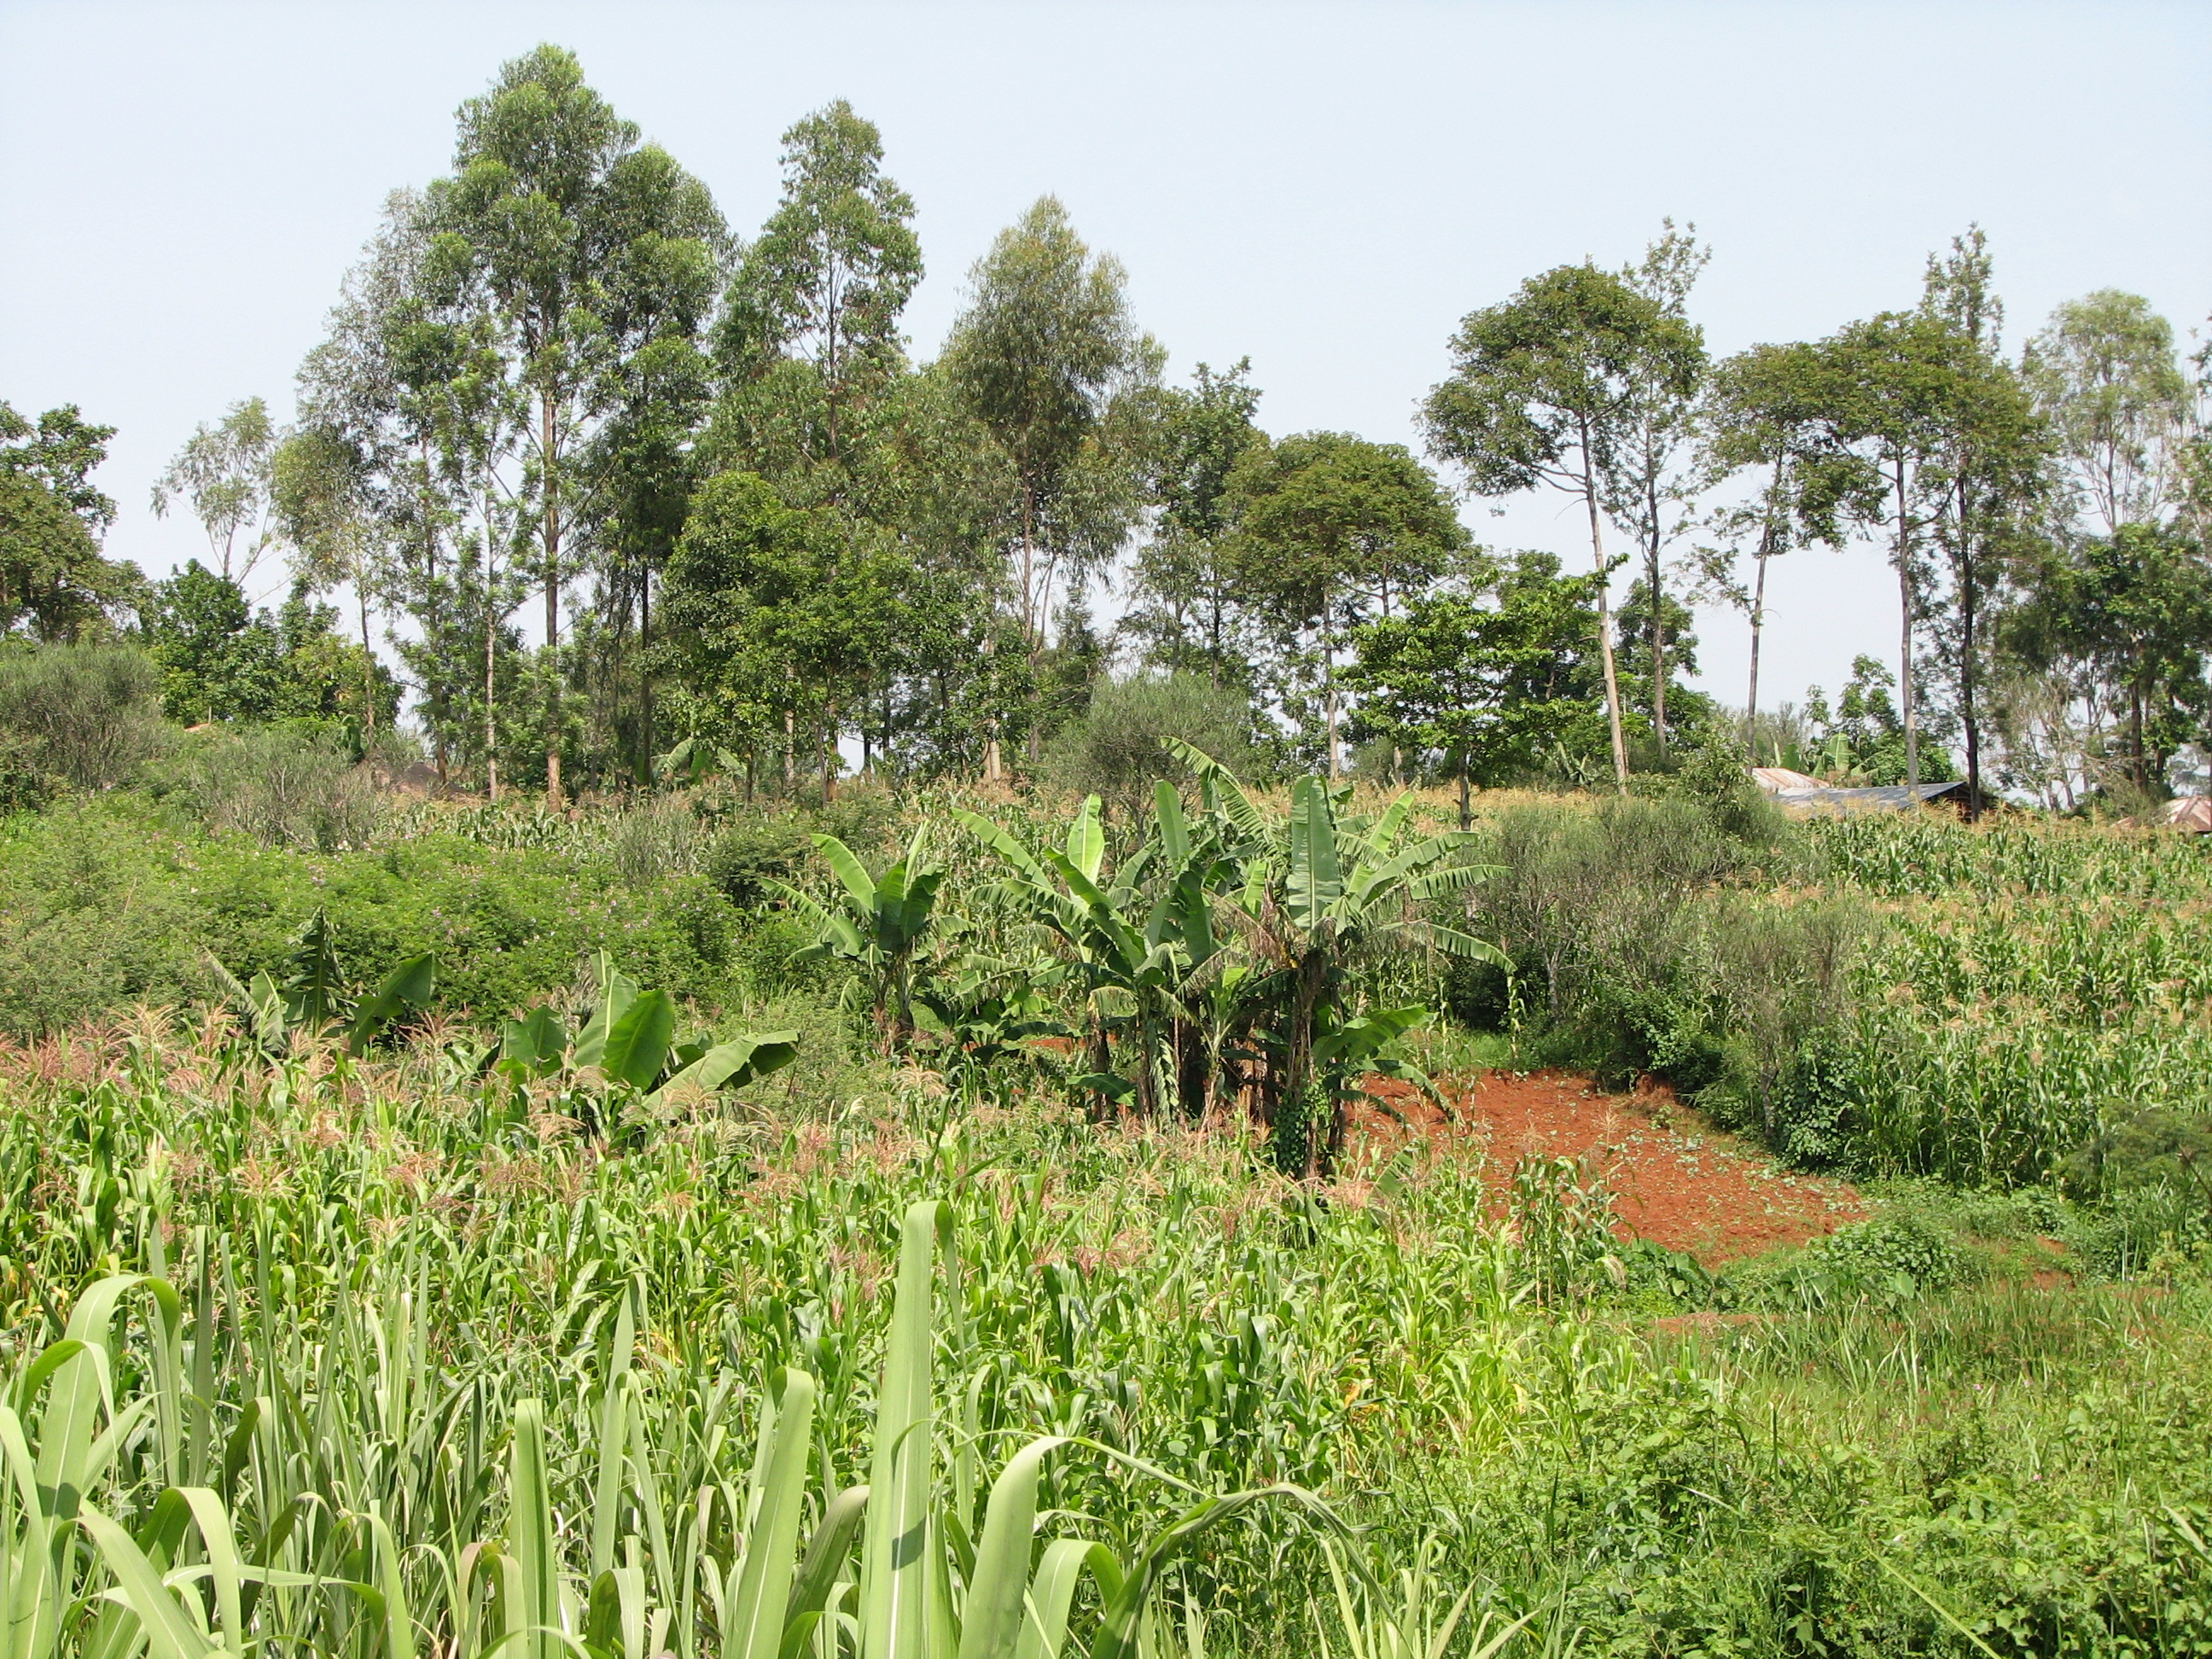
\includegraphics[keepaspectratio,width=1.6cm]{photos/sauri-crops.jpg}};
	\node [yellow,anchor=south west,align=left] at ([xshift=0.05cm,yshift=0.05cm]crops.south west)  {\tiny{agriculture}};
	%\node [anchor=north] (health) at (1.25,1.625)  {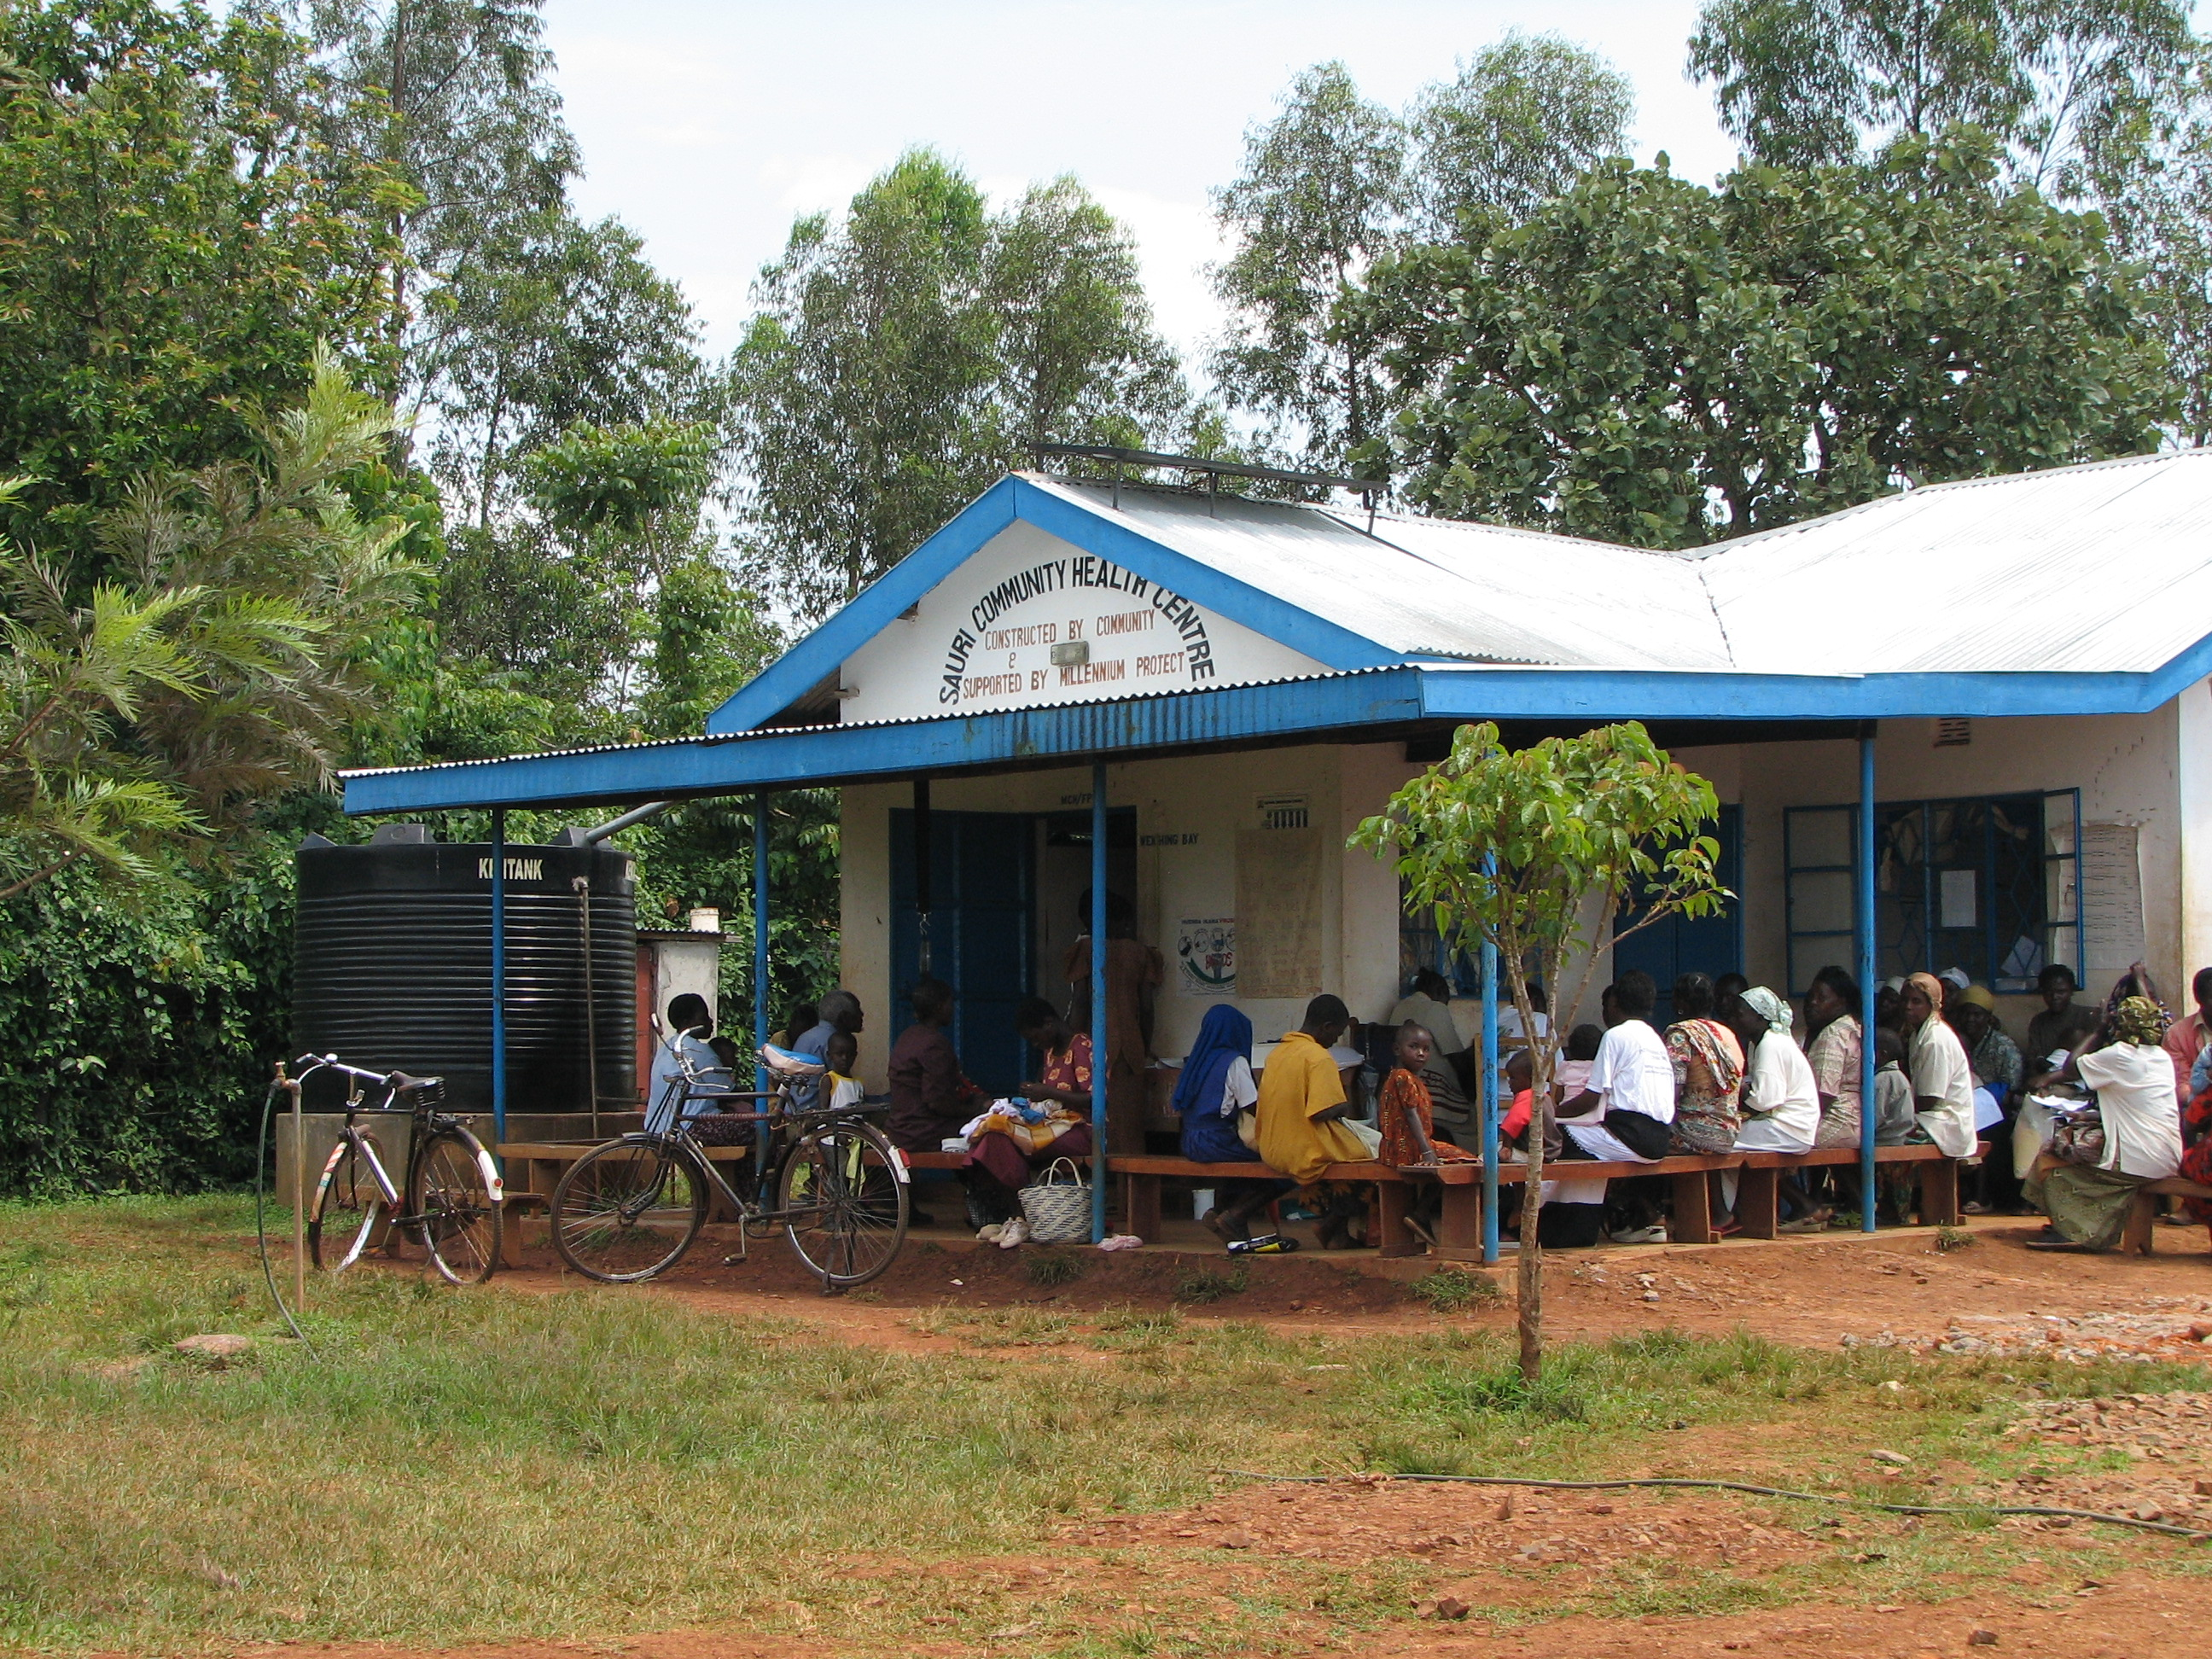
\includegraphics[keepaspectratio,width=1.6cm]{photos/sauri-health-center.jpg}};
	%\node [yellow,anchor=south west,align=left] at ([xshift=0.05cm,yshift=0.05cm]health.south west)  {\tiny{health}};
	
	\end{tikzpicture}
\end{center}
\end{frame}


%%%%%%%%%%%%%%%%%%%%%%%%%%%%%%%%%%%%%%%%%%%%%%%%%%%%%%%%%%%%%%%%%%%%%%%

\begin{frame}<handout:0>{The Millennium Villages Project:  A Big Push}

\begin{center}
	\begin{tikzpicture}
	
	% blank canvas
	\only<handout>{\fill[fill=white,draw=white,ultra thin]
		(0,0) -- (11,0) -- (11,6) -- (0,6) -- cycle;}
	\only<beamer>{\fill[fill=white,draw=white,ultra thin]
		(0,0) -- (14,0) -- (14,6) -- (0,6) -- cycle;}
	\only<beamer>{\draw[draw=oiblue!60,fill=oiblue!10,opacity=0.5] (11,1) rectangle (14,5);}
	%\draw[step=1.0,gray!20,thin] (0,0) grid (11,6);
	
	%	\pgfmathsetmacro\xshift{0.5cm};
	%	\pgfmathsetmacro\yshift{5.5cm};
	%	\pgfmathsetmacro\mycolor{"gray"};
	
	\node [anchor=north] (pronykF1) at (6,6)  {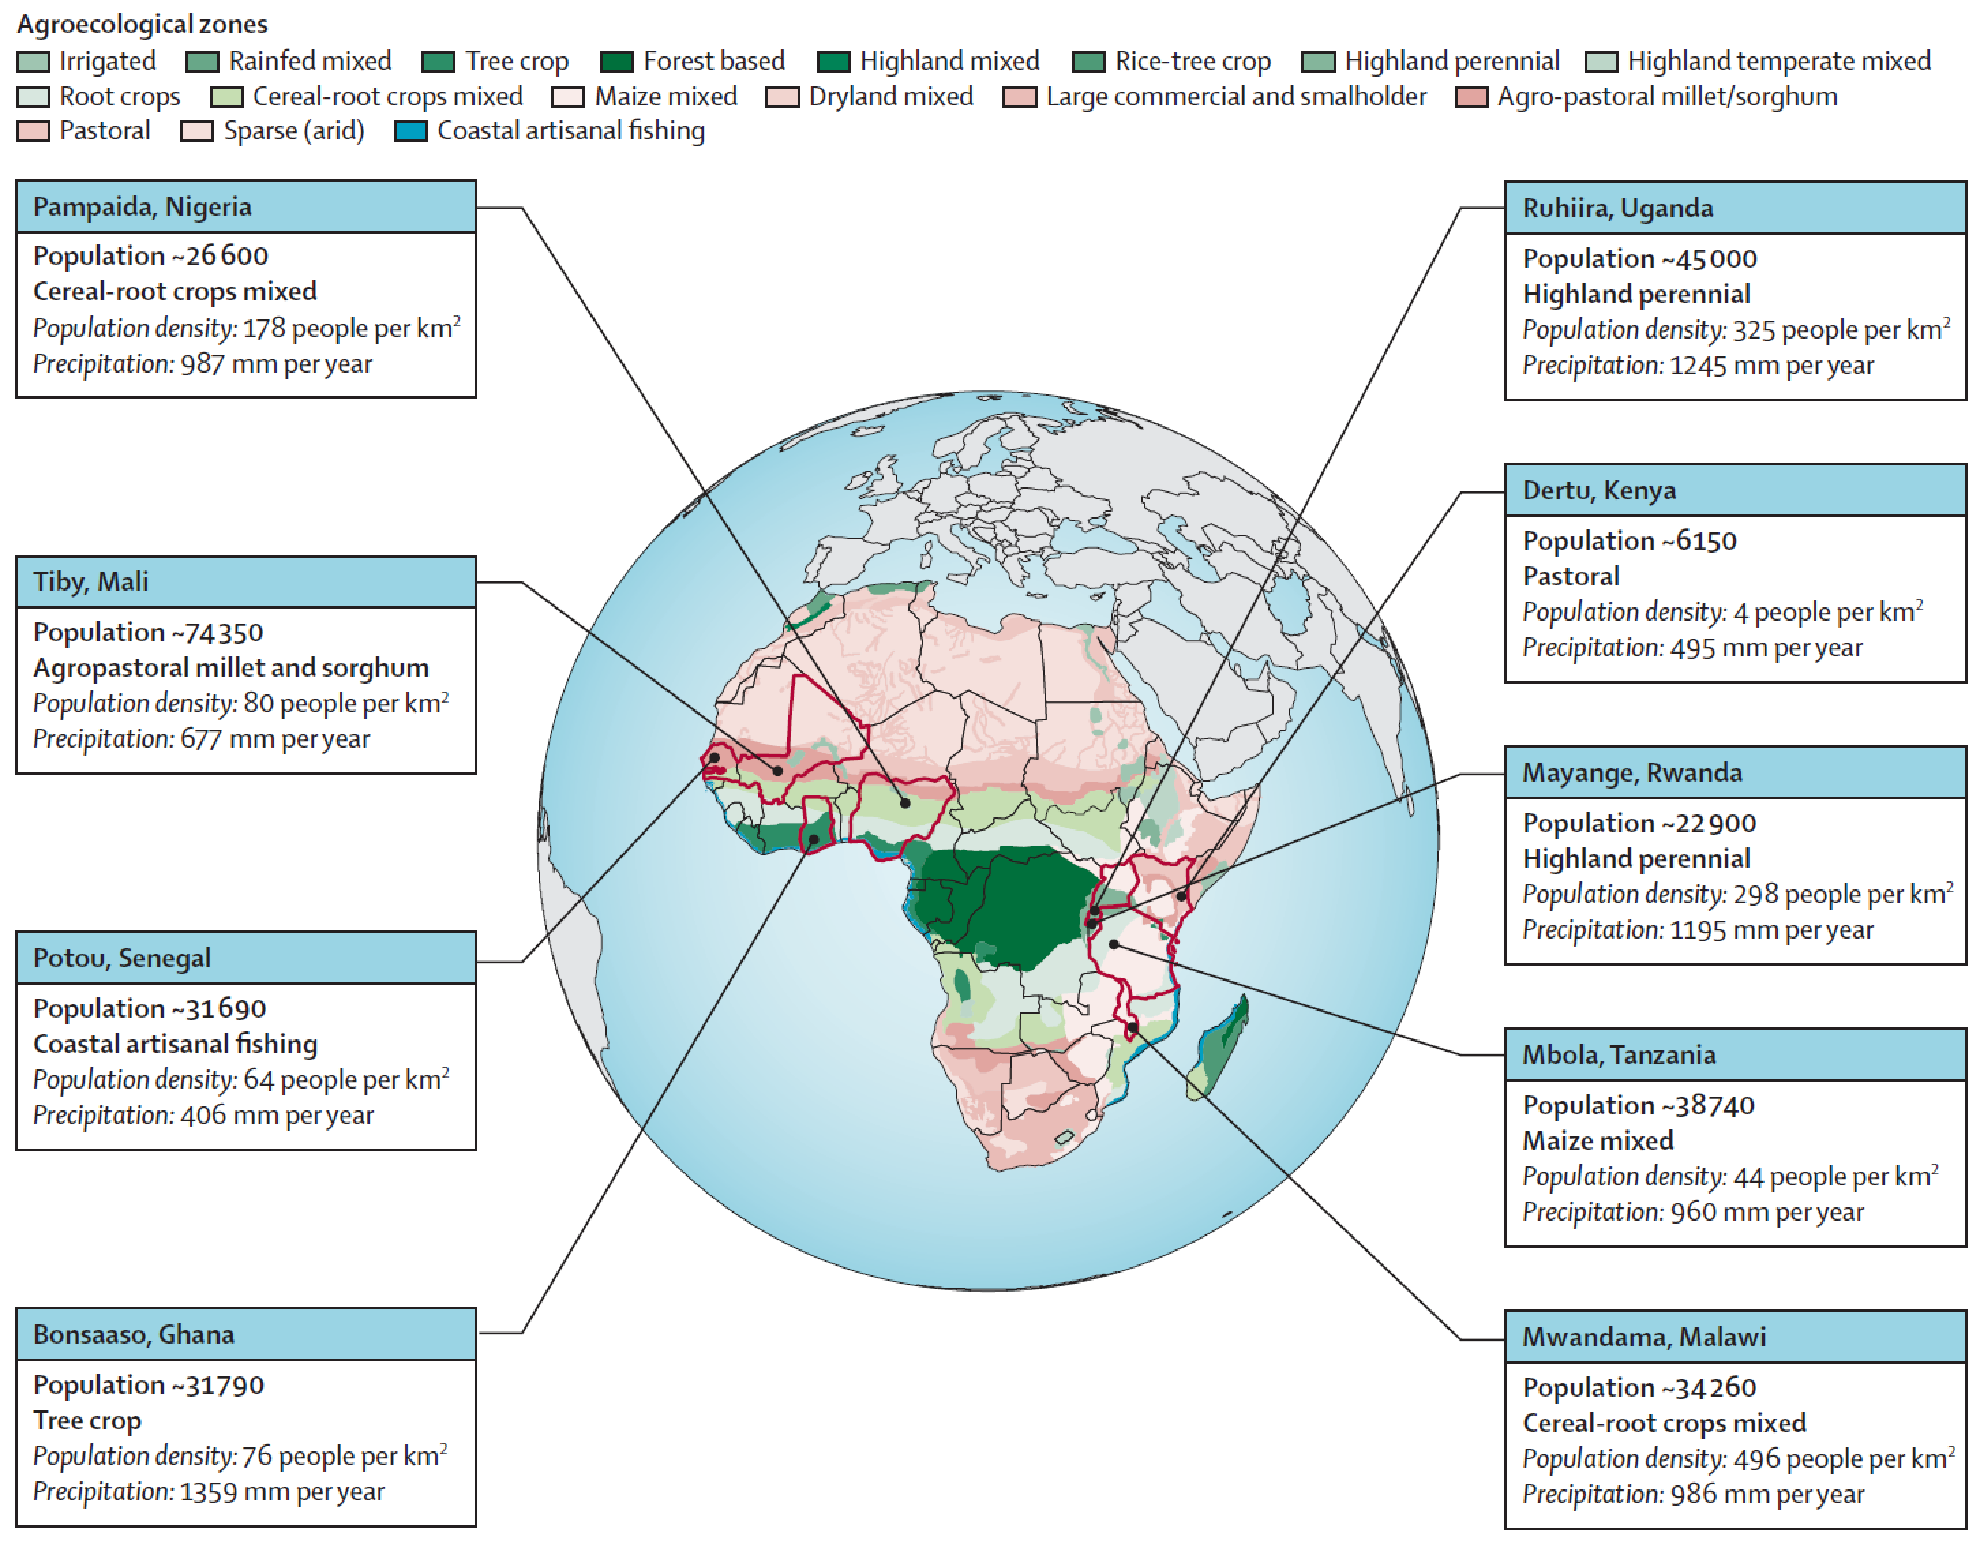
\includegraphics[keepaspectratio,width=7.2cm]{img/MVPmap.pdf}};
	\node [gray,anchor=north] at ([yshift=0.25cm]pronykF1.south)  {\tiny{source:  Pronyk et al.~(2012)}};
	
	\node [anchor=north] (sachs) at (1.25,6)  {
\includegraphics[keepaspectratio,width=2cm]{photos/sachs-rick-bajornas.jpg}};
	\node [gray,anchor=north] at ([yshift=0.125cm]sachs.south)  {\tiny{photo:  Rick Bajornas}};
	\node [anchor=north] (school) at (1.25,4.375)  {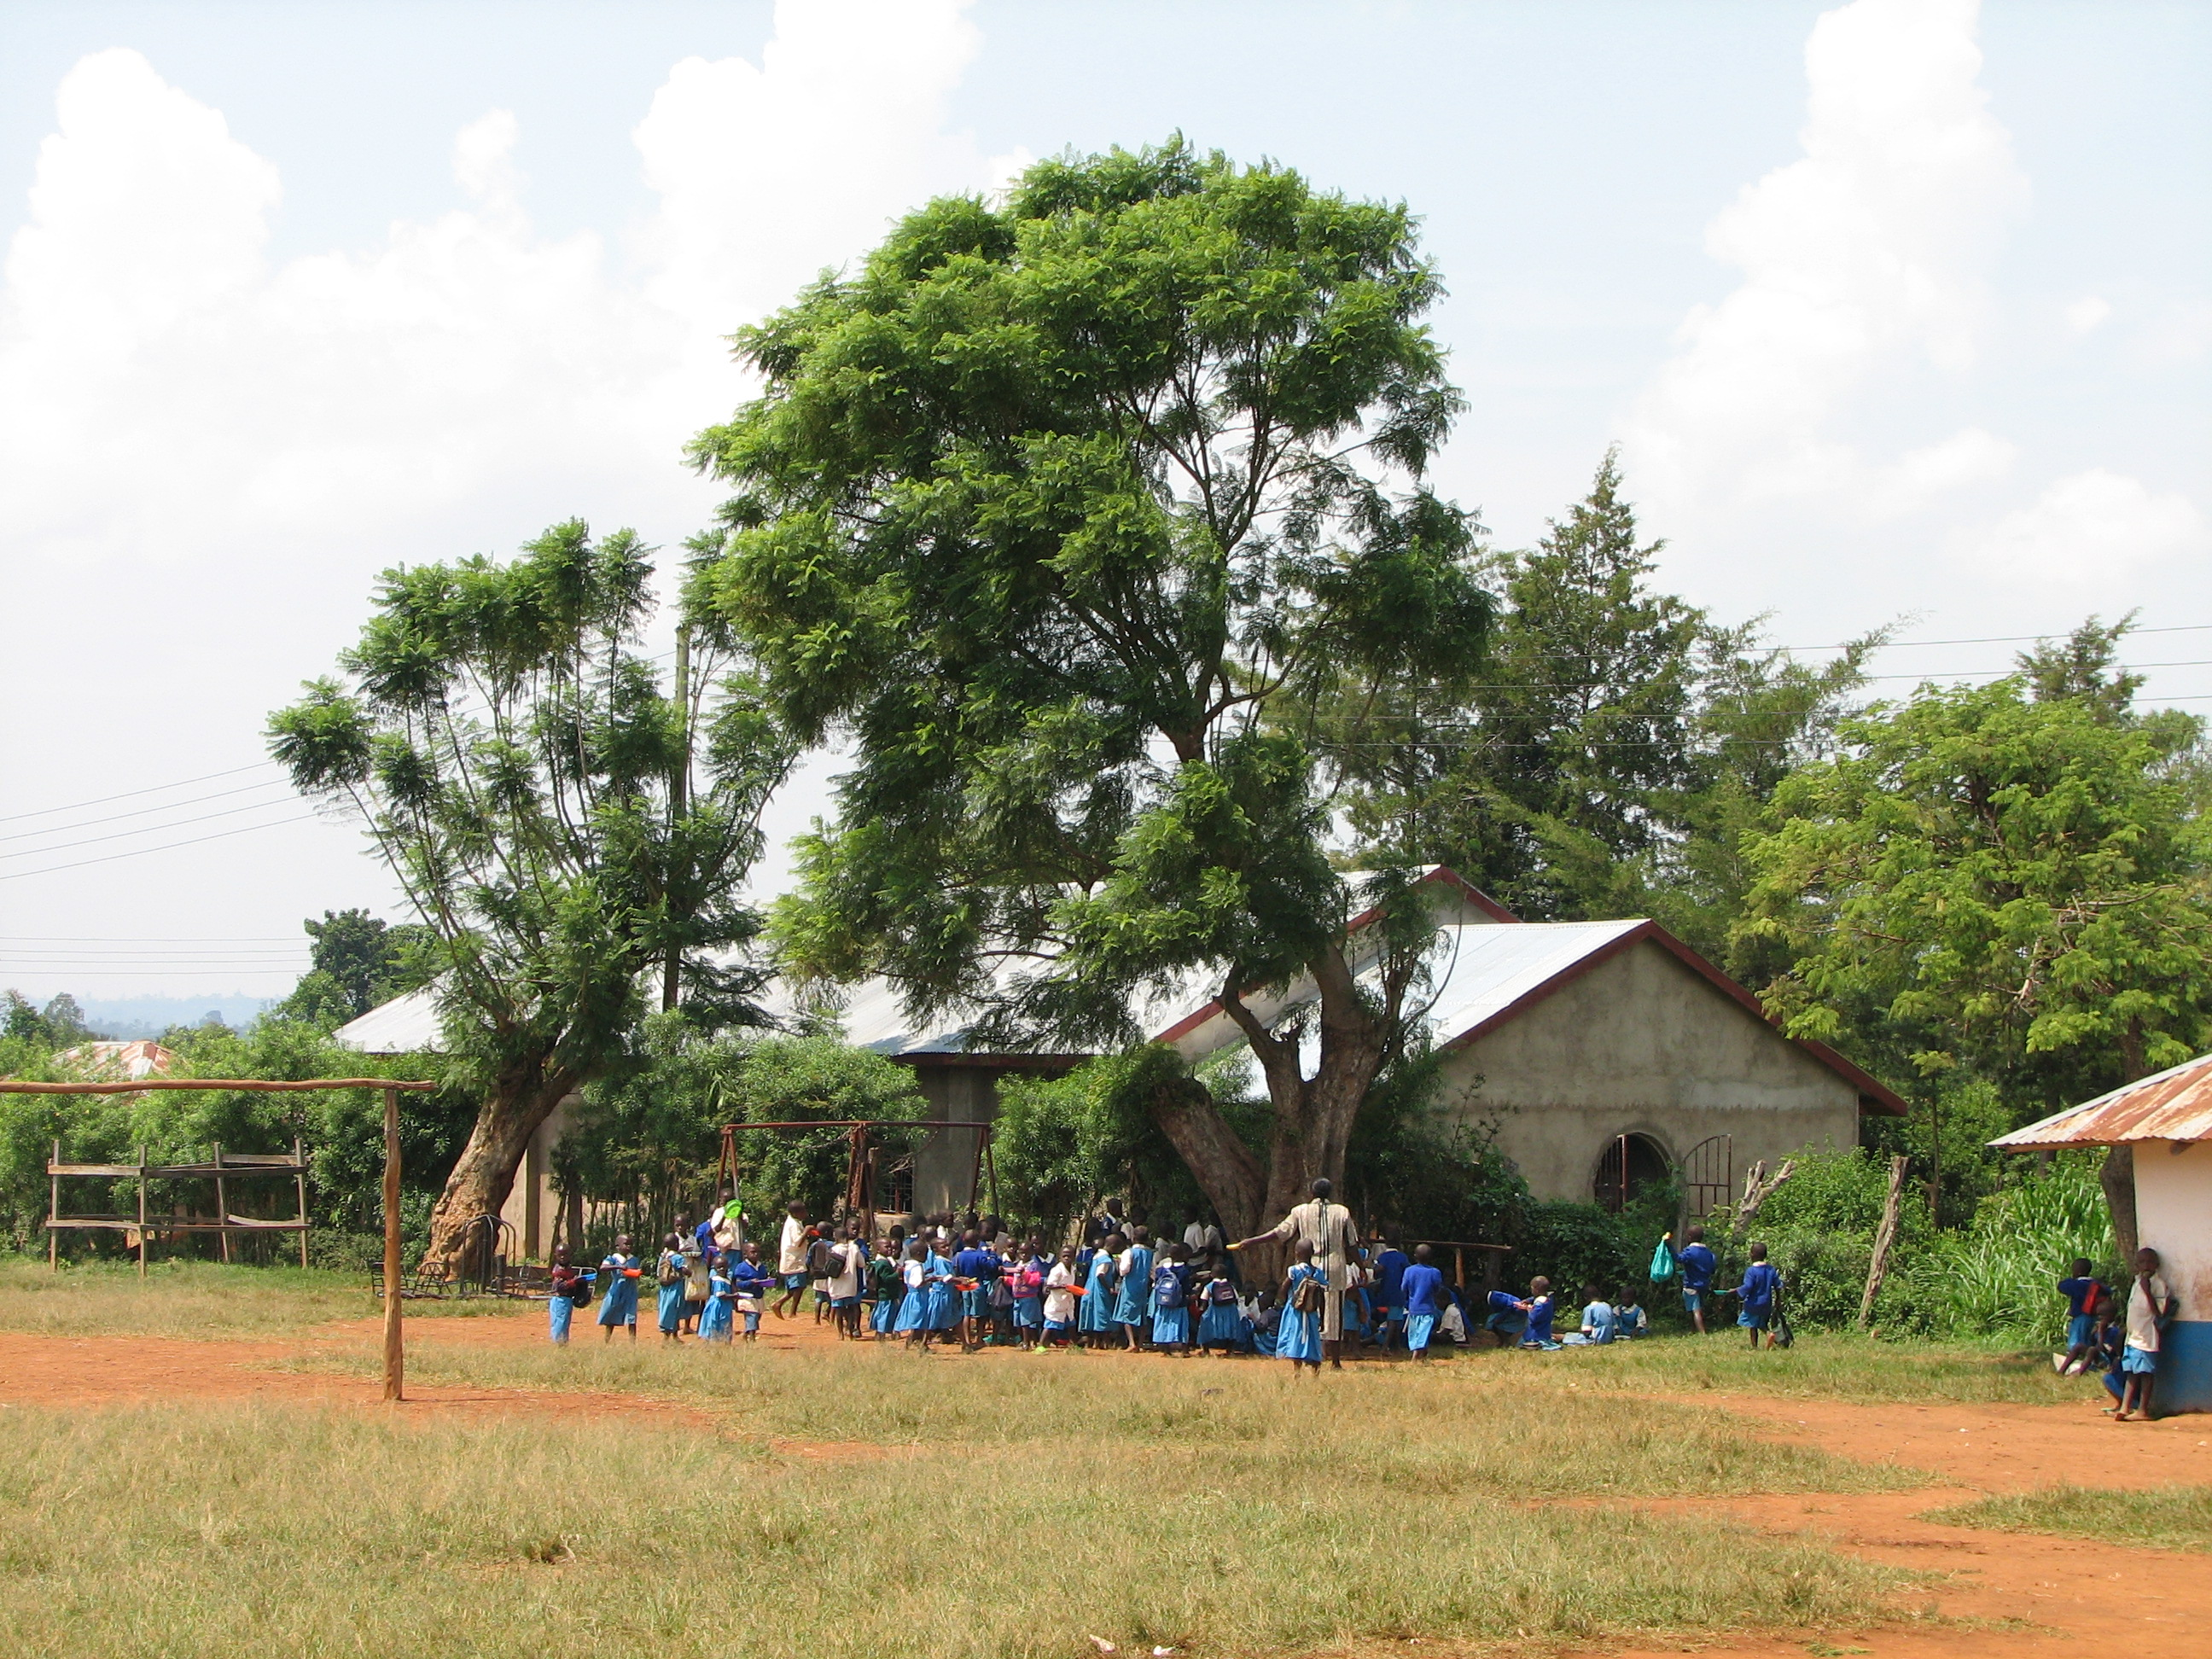
\includegraphics[keepaspectratio,width=1.6cm]{photos/sauri-primary.jpg}};
	\node [yellow,anchor=south west,align=left] at ([xshift=0.05cm,yshift=0.05cm]school.south west)  {\tiny{schools}};
	\node [anchor=north] (crops) at (1.25,3)  {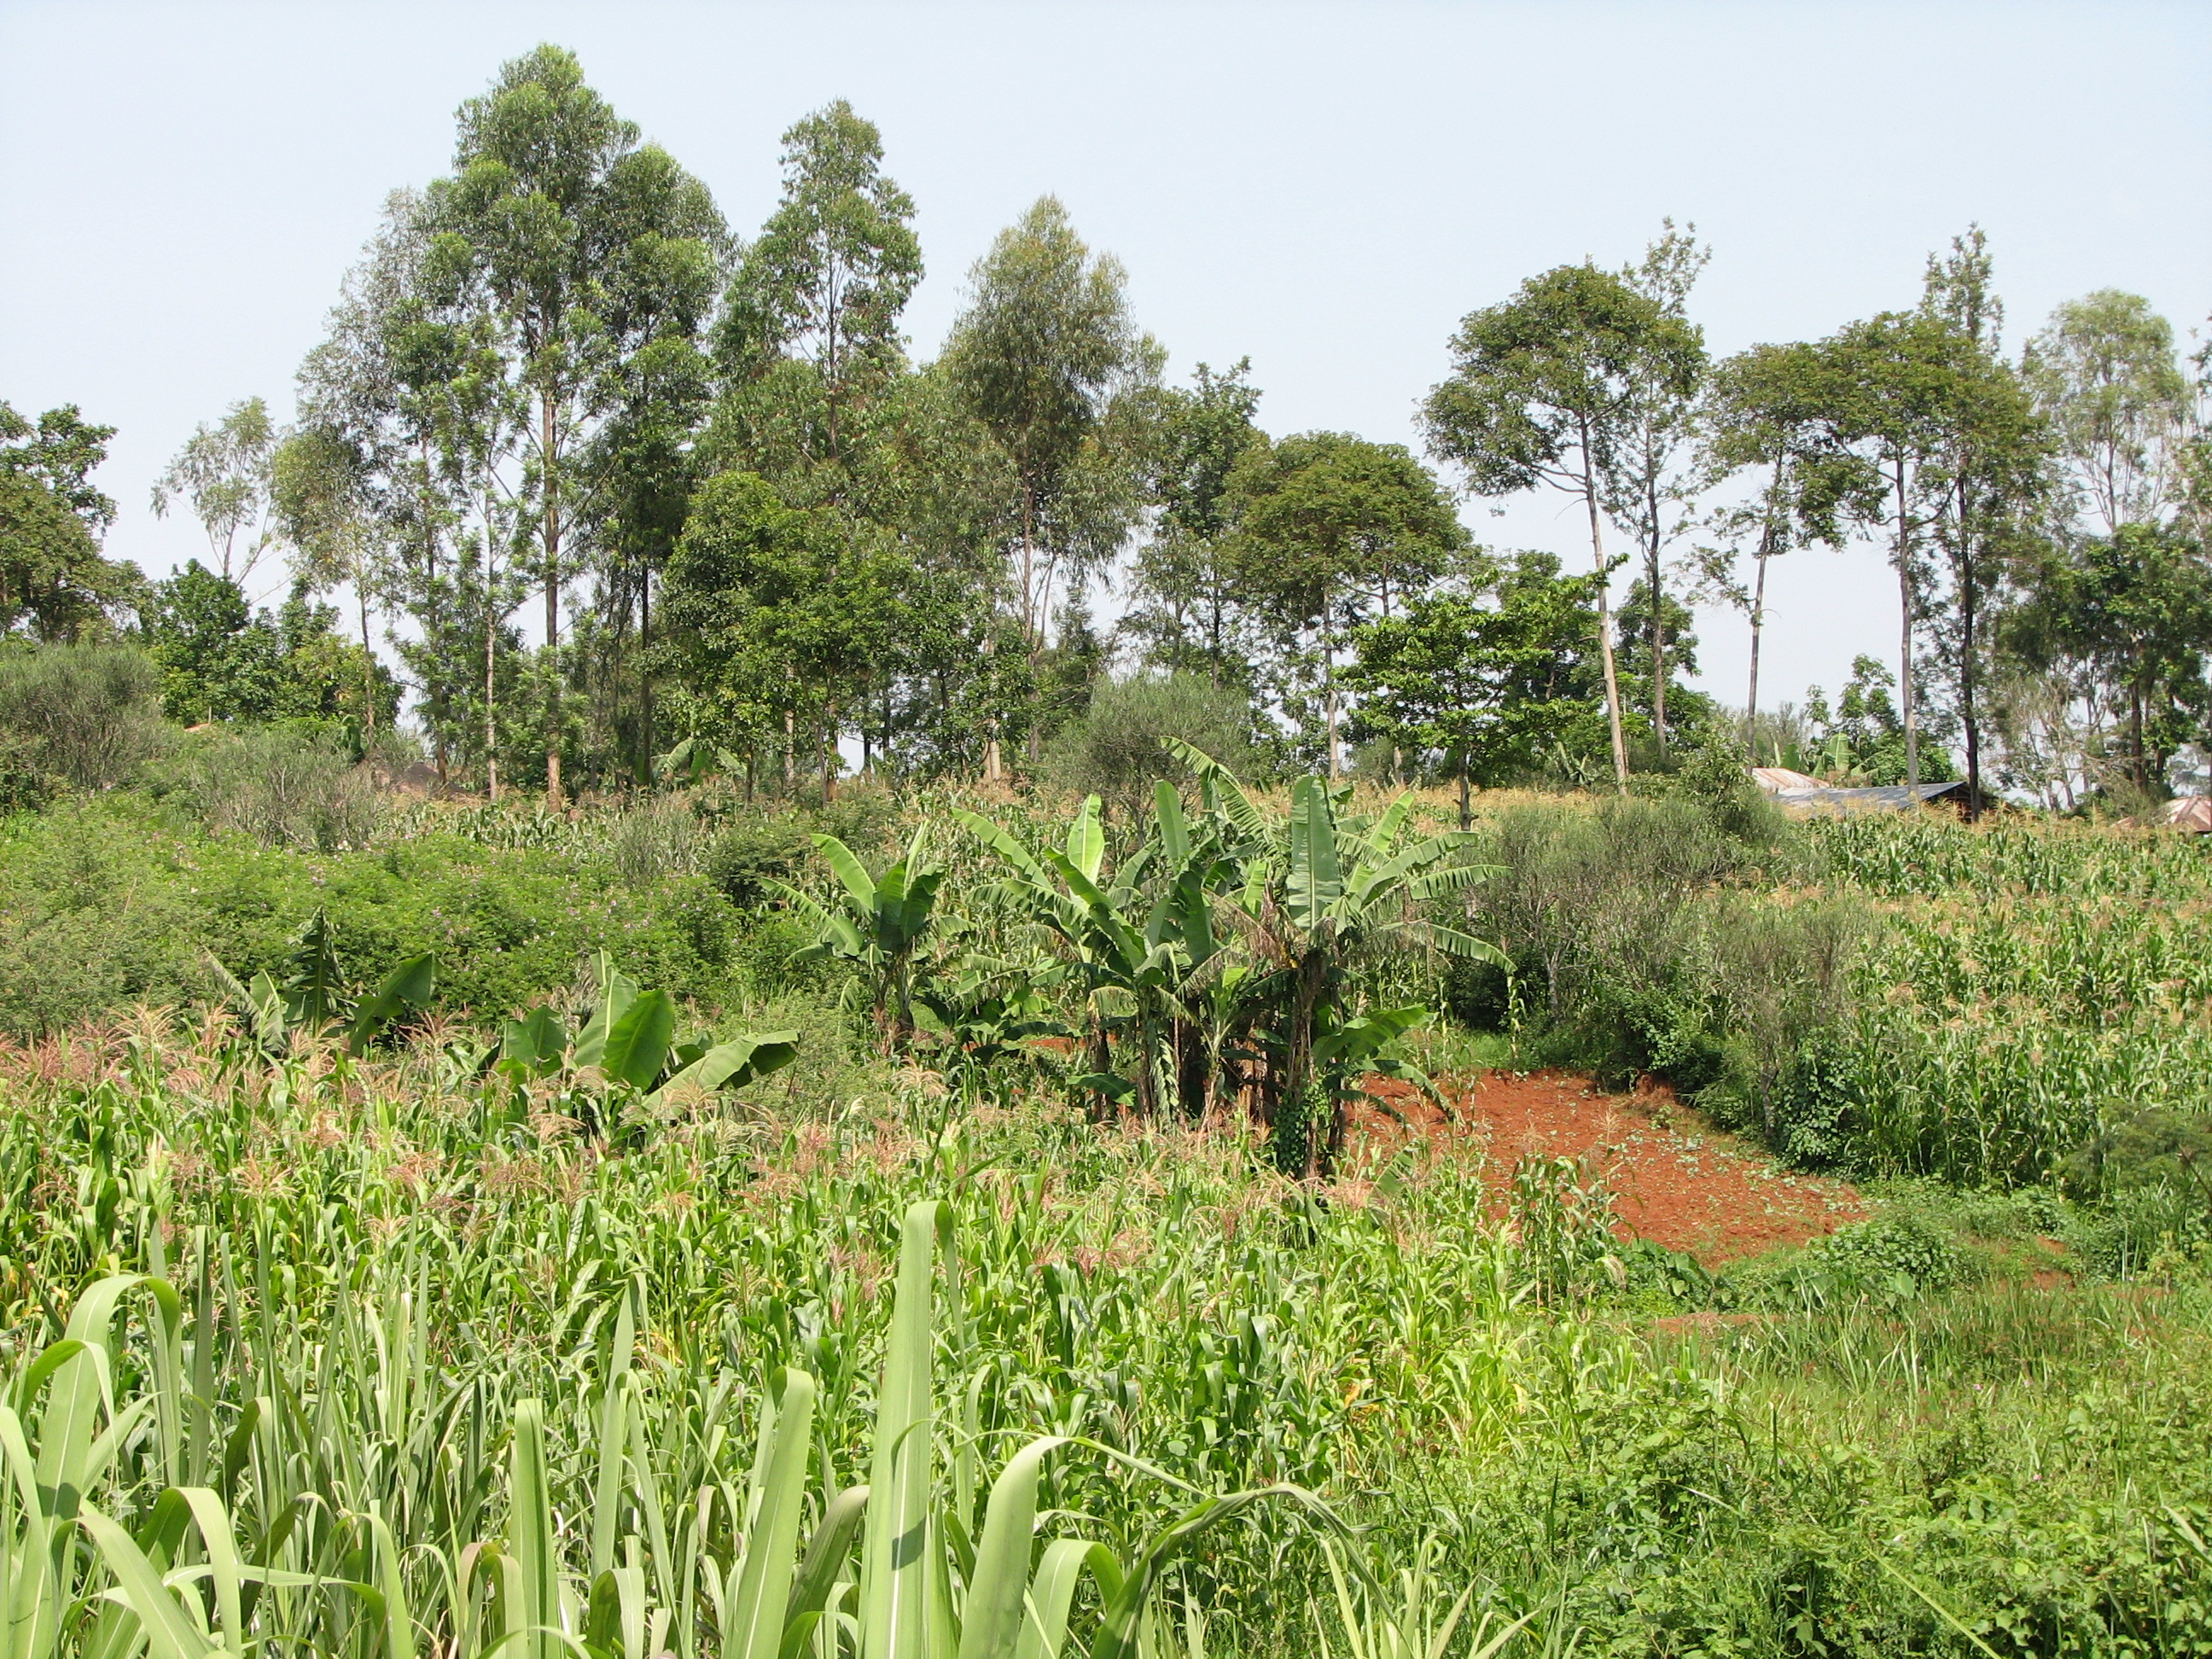
\includegraphics[keepaspectratio,width=1.6cm]{photos/sauri-crops.jpg}};
	\node [yellow,anchor=south west,align=left] at ([xshift=0.05cm,yshift=0.05cm]crops.south west)  {\tiny{agriculture}};
	\node [anchor=north] (health) at (1.25,1.625)  {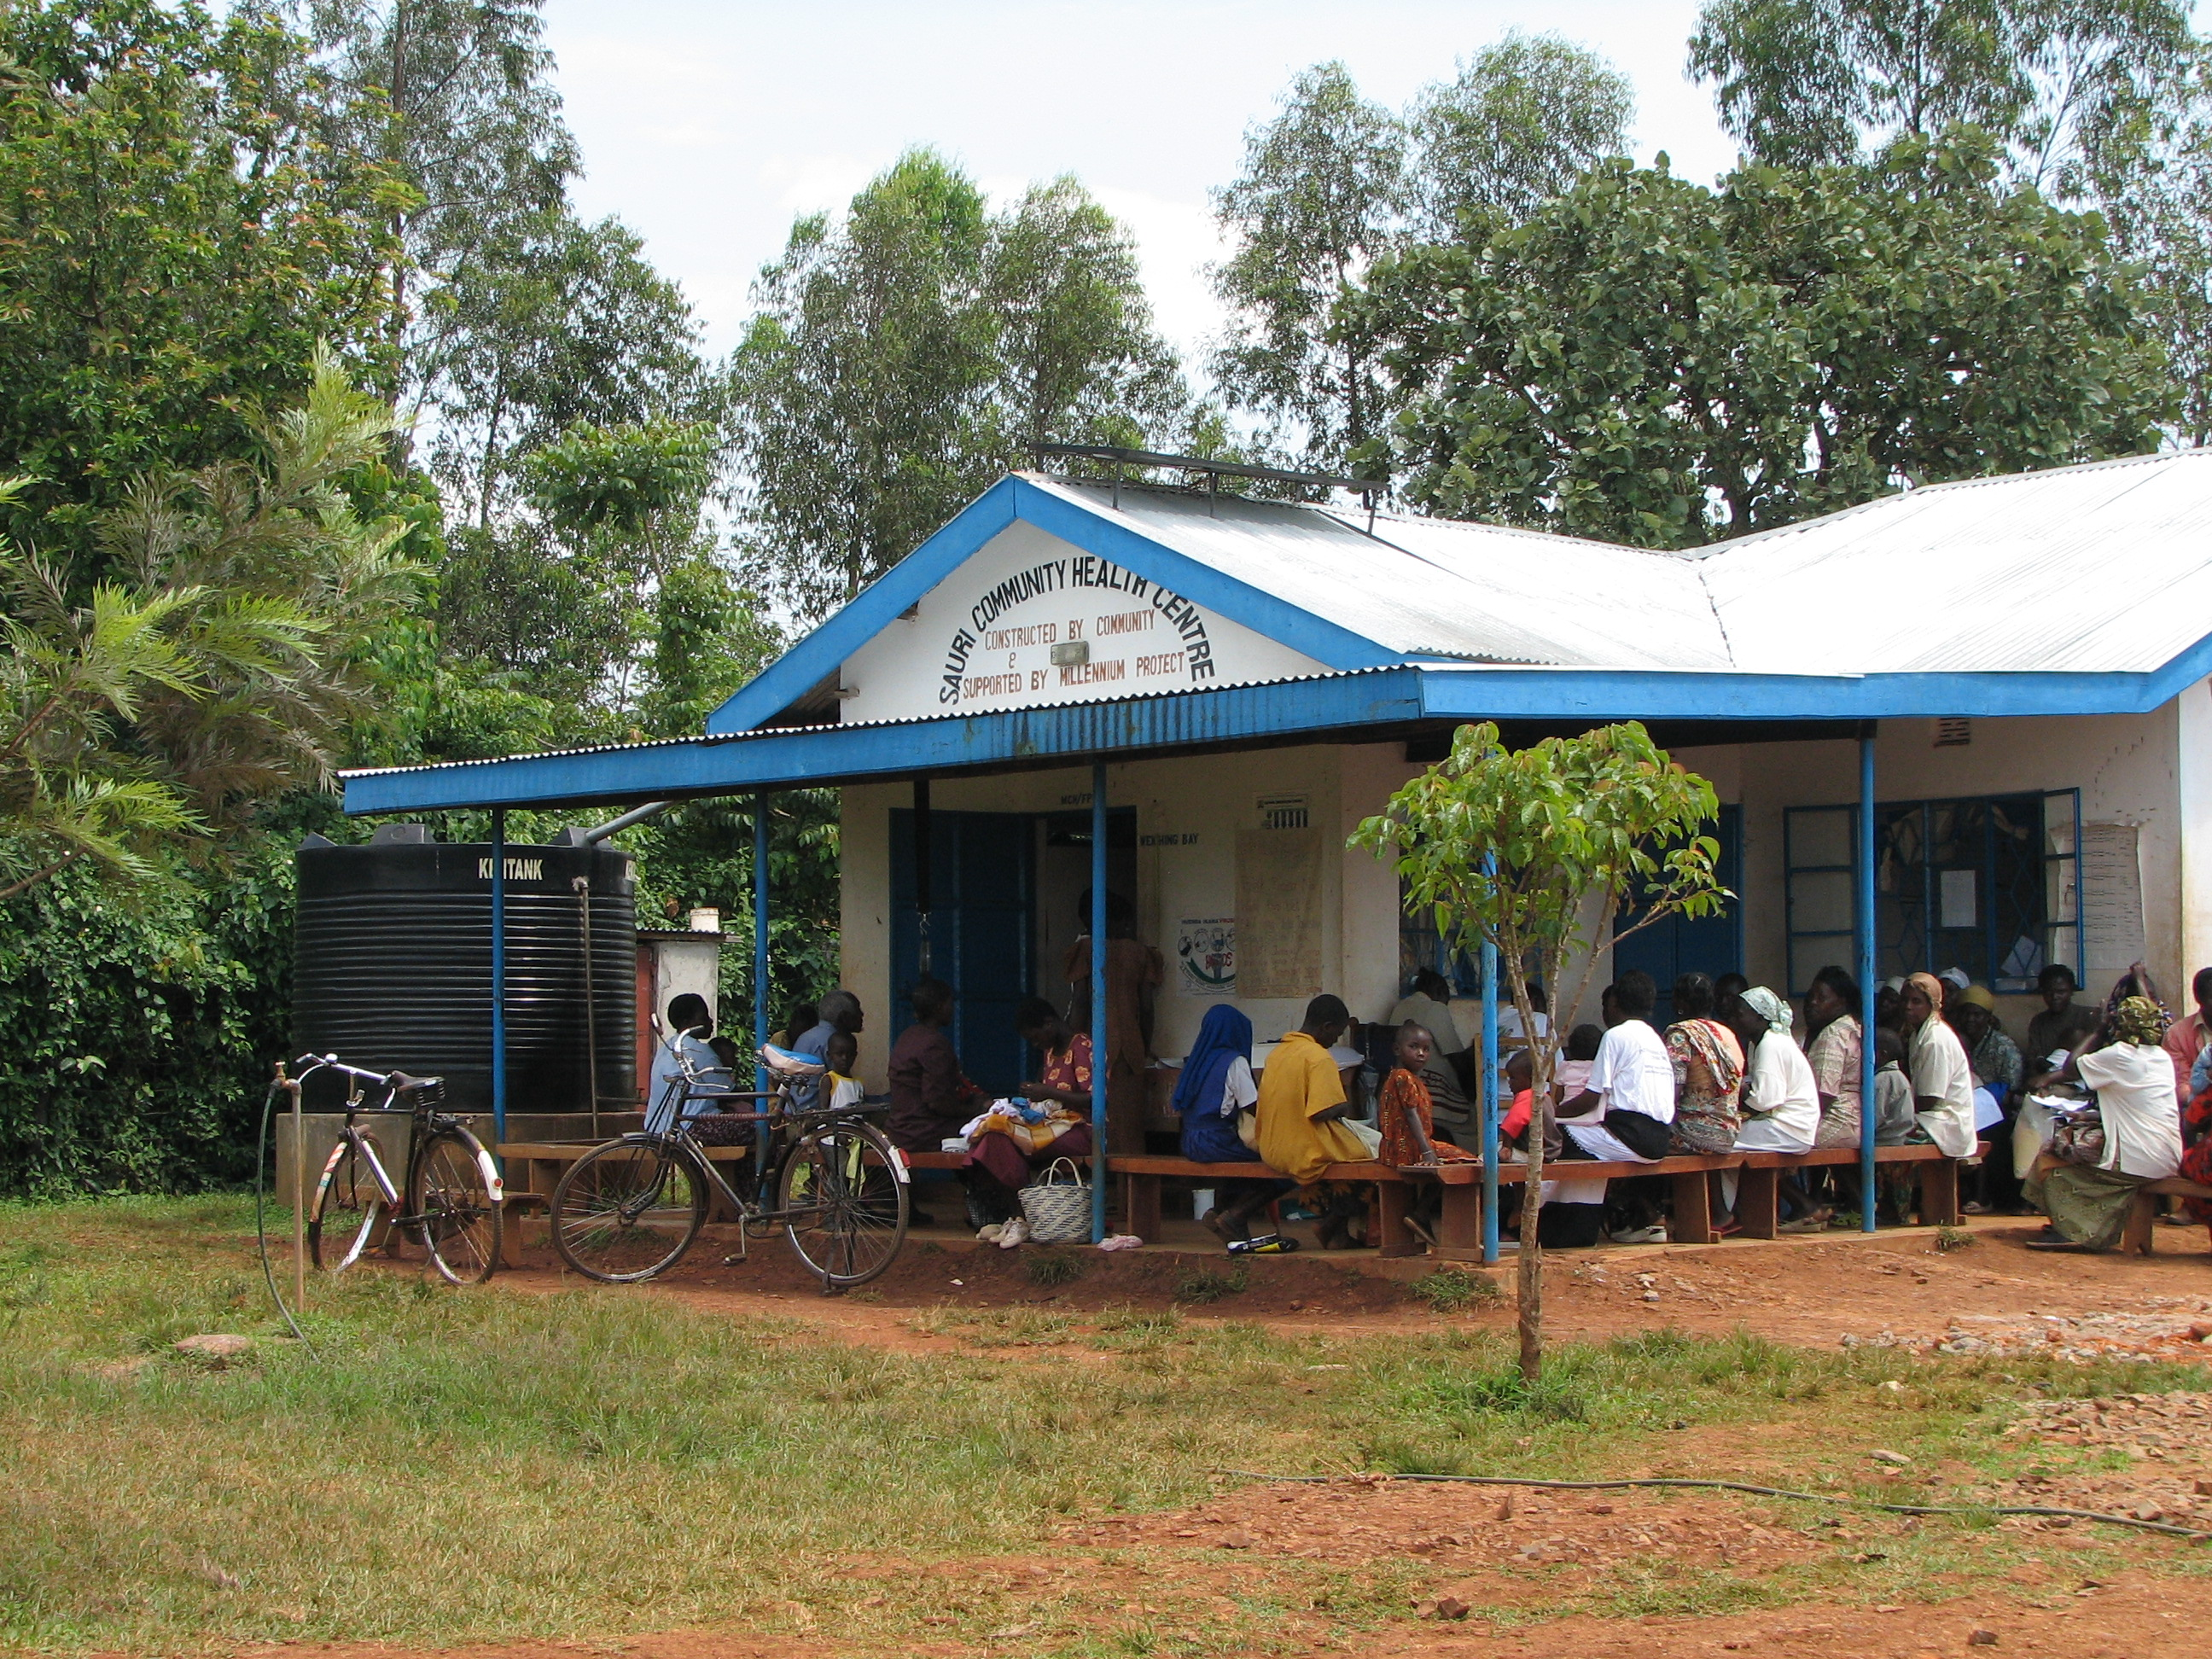
\includegraphics[keepaspectratio,width=1.6cm]{photos/sauri-health-center.jpg}};
	\node [yellow,anchor=south west,align=left] at ([xshift=0.05cm,yshift=0.05cm]health.south west)  {\tiny{health}};
	
	\end{tikzpicture}
\end{center}
\end{frame}



%%%%%%%%%%%%%%%%%%%%%%%%%%%%%%%%%%%%%%%%%%%%%%%%%%%%%%%%%%%%%%%%%%%%%%%

\begin{frame}<handout:0>{The Millennium Villages Project:  Per Capita Spending}

\begin{center}
	\begin{tikzpicture}
	
	% blank canvas
	\only<handout>{\fill[fill=white,draw=white,ultra thin]
		(0,0) -- (11,0) -- (11,6) -- (0,6) -- cycle;}
	\only<beamer>{\fill[fill=white,draw=white,ultra thin]
		(0,0) -- (14,0) -- (14,6) -- (0,6) -- cycle;}
	\only<beamer>{\draw[draw=oiblue!60,fill=oiblue!10,opacity=0.5] (11,1) rectangle (14,5);}
	%\draw[step=1.0,gray!20,thin] (0,0) grid (11,6);
	
	%	\pgfmathsetmacro\xshift{0.5cm};
	%	\pgfmathsetmacro\yshift{5.5cm};
	%	\pgfmathsetmacro\mycolor{"gray"};
	
	\node [anchor=north] (pronykF3) at (5,6)  {\fbox{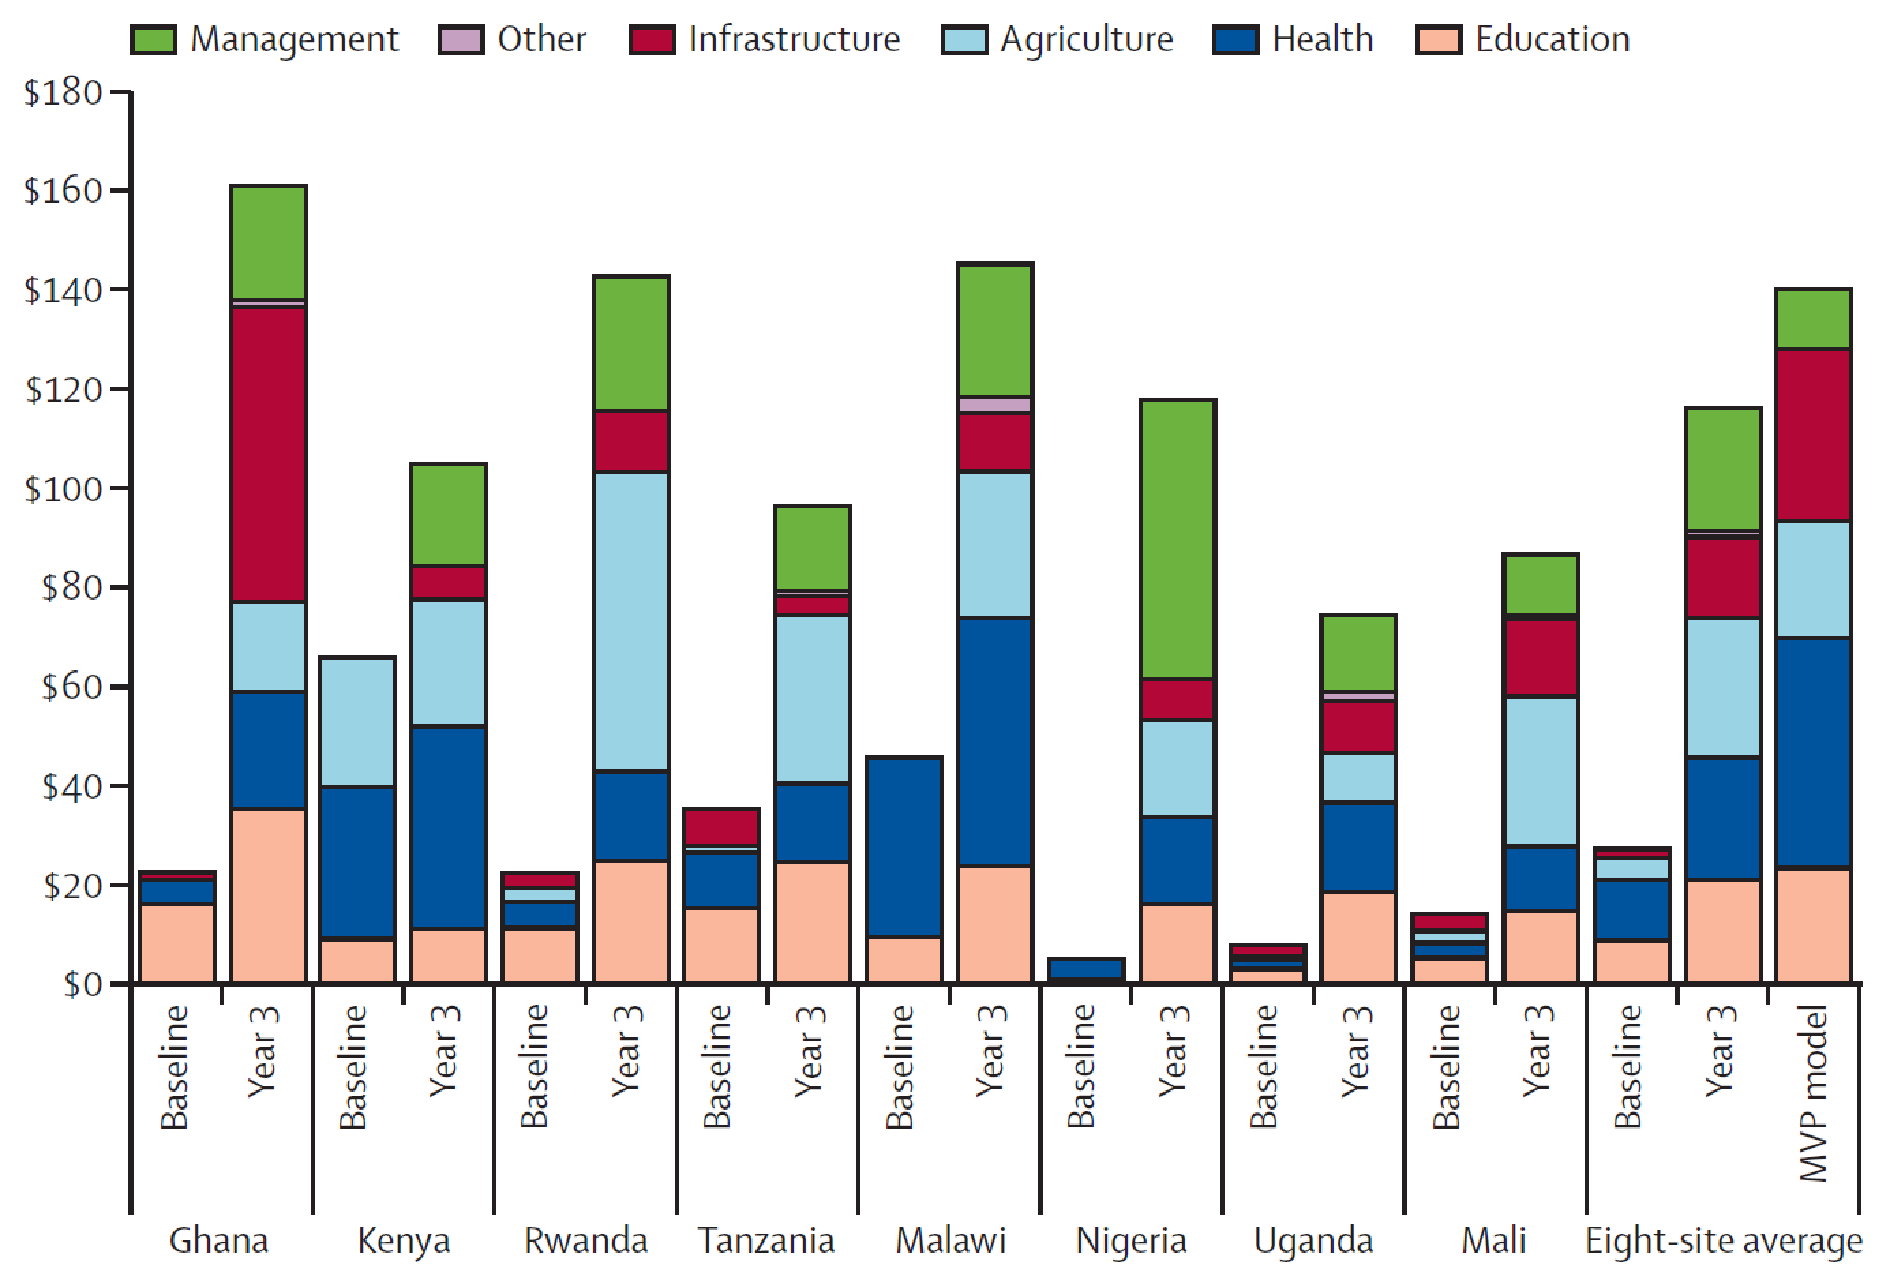
\includegraphics[keepaspectratio,width=7.2cm]{img/MVPspending.pdf}}};
	\node [gray,anchor=north] at ([yshift=0.125cm]pronykF3.south)  {\tiny{source:  Pronyk et al.~(2012)}};
	
	\end{tikzpicture}
\end{center}
\end{frame}



%%%%%%%%%%%%%%%%%%%%%%%%%%%%%%%%%%%%%%%%%%%%%%%%%%%%%%%%%%%%%%%%%%%%%%%

\begin{frame}{The Impacts of the Millennium Villages Project?}

\begin{center}
	\begin{tikzpicture}
	
	% blank canvas
	%\only<handout>{\fill[fill=white,draw=white,ultra thin]	(0,0) -- (11,0) -- (11,6) -- (0,6) -- cycle;}
	%\only<beamer>{\fill[fill=white,draw=white,ultra thin]	(0,0) -- (14,0) -- (14,6) -- (0,6) -- cycle;}
	\fill[fill=white,draw=white,ultra thin] (0,0) -- (14,0) -- (14,6) -- (0,6) -- cycle;
	%\only<beamer>{\draw[draw=oiblue!60,fill=oiblue!10,opacity=0.5] (11,1) rectangle (14,5);}
	%\draw[step=1.0,gray!20,thin] (0,0) grid (14,6);
	
	%	\pgfmathsetmacro\xshift{0.5cm};
	%	\pgfmathsetmacro\yshift{5.5cm};
	%	\pgfmathsetmacro\mycolor{"gray"};
	
	\node [anchor=north east] (tab1) at (6.95,5.75)  {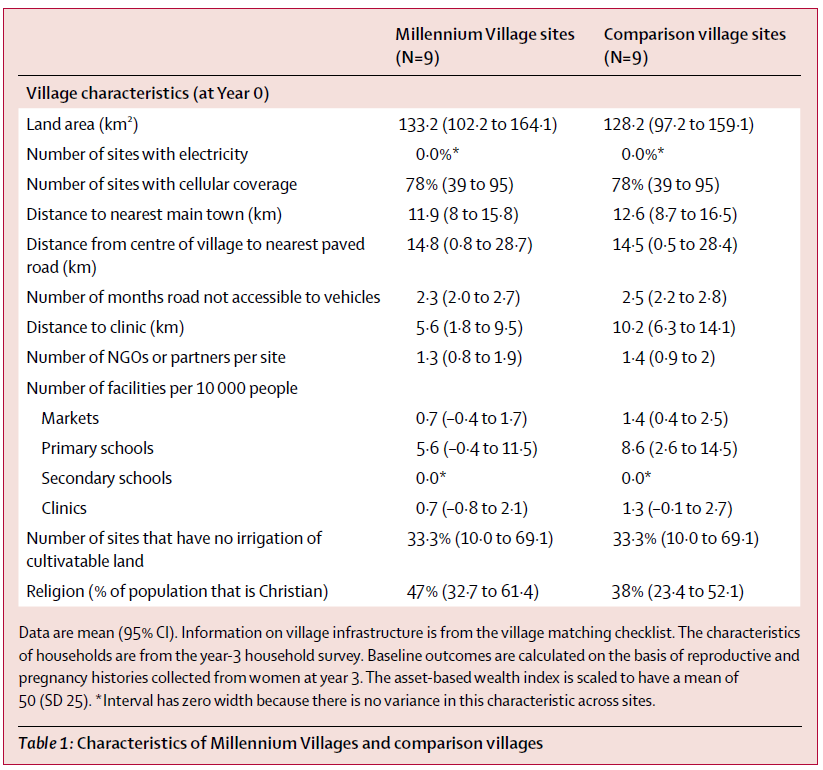
\includegraphics[keepaspectratio,width=5.2cm]{img/pronyk-stats1.png}};
	\node [anchor=north west] (tab2) at (7.05,5.75)  {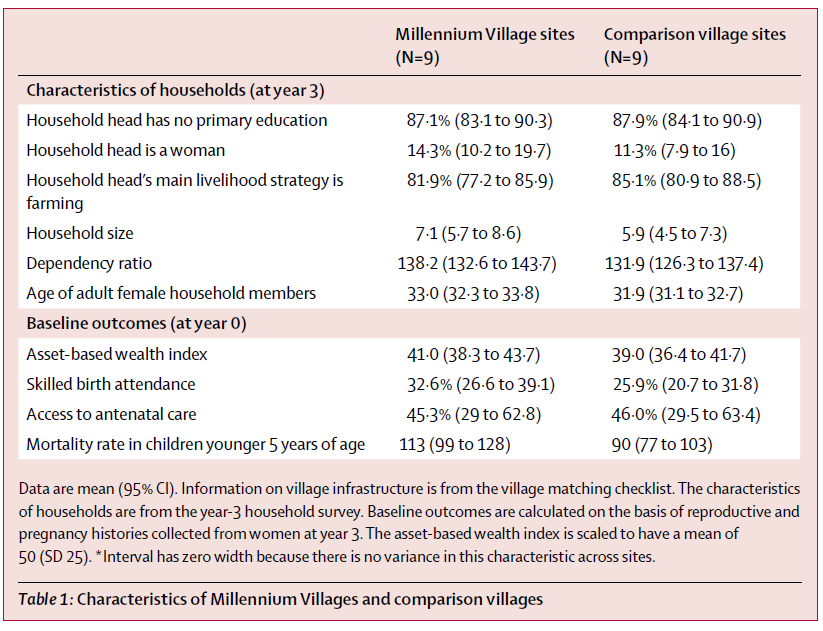
\includegraphics[keepaspectratio,width=5.2cm]{img/pronyk-stats2.png}};
	
	\node [gray,anchor=north] at (tab1.south)  {\tiny{source:  Pronyk et al.~(2012)}};
	\node [gray,anchor=north] at (tab2.south)  {\tiny{source:  Pronyk et al.~(2012)}};
	
	\end{tikzpicture}
\end{center}
\end{frame}



%%%%%%%%%%%%%%%%%%%%%%%%%%%%%%%%%%%%%%%%%%%%%%%%%%%%%%%%%%%%%%%%%%%%%%%

\begin{frame}{The Impacts of the Millennium Villages Project?}

\begin{center}
	\begin{tikzpicture}
	
	% blank canvas
	%\only<handout>{\fill[fill=white,draw=white,ultra thin]	(0,0) -- (11,0) -- (11,6) -- (0,6) -- cycle;}
	%\only<beamer>{\fill[fill=white,draw=white,ultra thin]	(0,0) -- (14,0) -- (14,6) -- (0,6) -- cycle;}
	\fill[fill=white,draw=white,ultra thin] (0,0) -- (14,0) -- (14,6) -- (0,6) -- cycle;
	%\only<beamer>{\draw[draw=oiblue!60,fill=oiblue!10,opacity=0.5] (11,1) rectangle (14,5);}
	%\draw[step=1.0,gray!20,thin] (0,0) grid (14,6);
	
	%	\pgfmathsetmacro\xshift{0.5cm};
	%	\pgfmathsetmacro\yshift{5.5cm};
	%	\pgfmathsetmacro\mycolor{"gray"};
	
	\node [anchor=north] (tab1) at (7,5.75)  {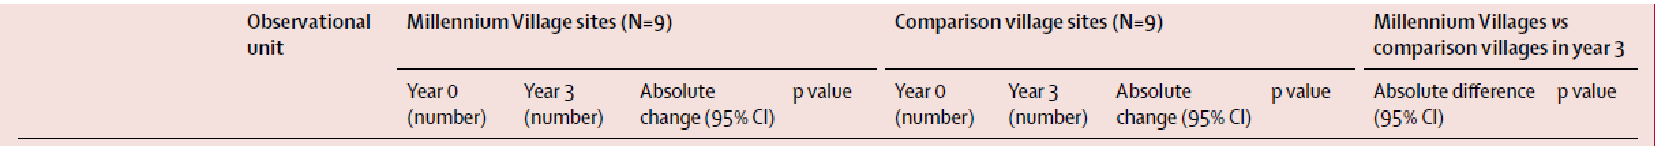
\includegraphics[keepaspectratio,width=10cm]{img/MVPimpacts-header.pdf}};
	\node [anchor=north] (tab2) at ([yshift=0.3cm]tab1.south)  {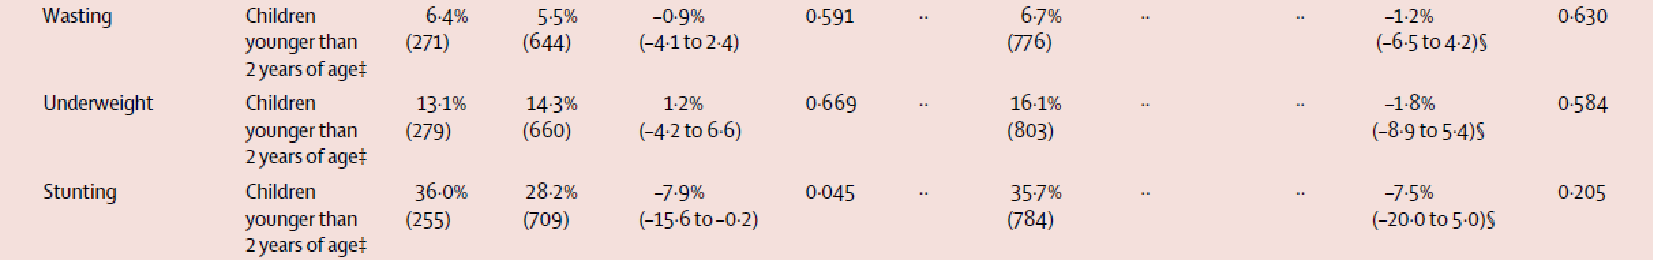
\includegraphics[keepaspectratio,width=10cm]{img/MVPimpacts-health.pdf}};
	\node [anchor=north] (tab3) at ([yshift=0.32cm]tab2.south)  {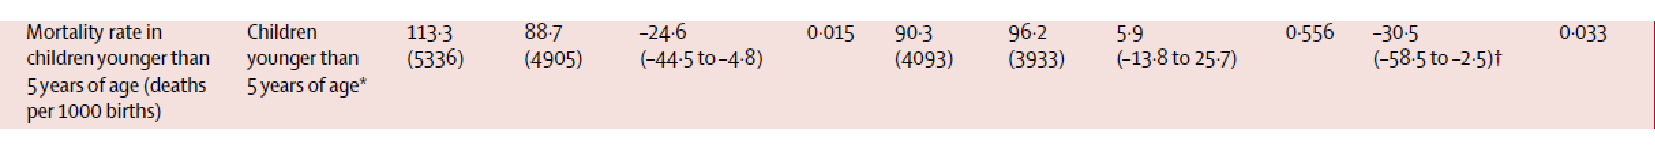
\includegraphics[keepaspectratio,width=10cm]{img/MVPimpacts-U5mortality.pdf}};	
	
	\filldraw[white] (1.95,2.25) rectangle (2.05,5.8);
	\filldraw[white] (11.95,2.25) rectangle (12.05,5.8);
	\node [gray,anchor=north] at ([yshift=0.125cm]tab3.south)  {\tiny{source:  Pronyk et al.~(2012)}};
	
	\end{tikzpicture}
\end{center}
\end{frame}


%%%%%%%%%%%%%%%%%%%%%%%%%%%%%%%%%%%%%%%%%%%%%%%%%%%%%%%%%%%%%%%%%%%%%%%

\begin{frame}{Critiques of the MVP Evaluation}

\begin{center}
	\begin{tikzpicture}
	
	% blank canvas
	%\only<handout>{\fill[fill=white,draw=white,ultra thin]	(0,0) -- (11,0) -- (11,6) -- (0,6) -- cycle;}
	%\only<beamer>{\fill[fill=white,draw=white,ultra thin]	(0,0) -- (14,0) -- (14,6) -- (0,6) -- cycle;}
	\fill[fill=white,draw=white,ultra thin] (0,0) -- (14,0) -- (14,6) -- (0,6) -- cycle;
	%\only<beamer>{\draw[draw=oiblue!60,fill=oiblue!10,opacity=0.5] (11,1) rectangle (14,5);}
	%\draw[step=1.0,gray!20,thin] (0,0) grid (14,6);
	
	%	\pgfmathsetmacro\xshift{0.5cm};
	%	\pgfmathsetmacro\yshift{5.5cm};
	%	\pgfmathsetmacro\mycolor{"gray"};
	
	\node [anchor=north west] (text1) at (0.25,5.5)  {Bump, Clemens, Demombynes, and Haddad (2012) raise three issues:};
	%	\node [anchor=north] (tab2) at ([yshift=0.3cm]tab1.south)  {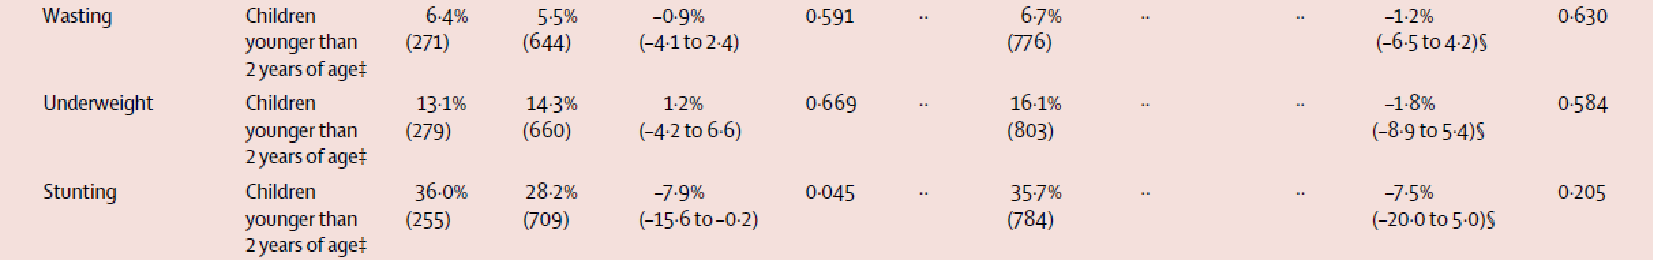
\includegraphics[keepaspectratio,width=10cm]{img/MVPimpacts-health.pdf}};
	%	\node [anchor=north] (tab3) at ([yshift=0.32cm]tab2.south)  {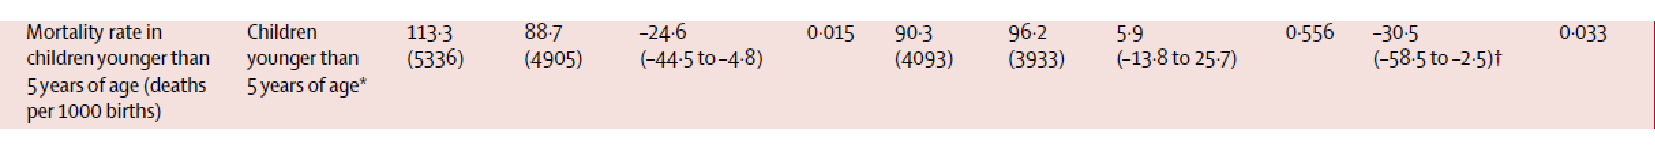
\includegraphics[keepaspectratio,width=10cm]{img/MVPimpacts-U5mortality.pdf}};	
	
	
	\end{tikzpicture}
\end{center}
\end{frame}




%%%%%%%%%%%%%%%%%%%%%%%%%%%%%%%%%%%%%%%%%%%%%%%%%%%%%%%%%%%%%%%%%%%%%%%

\begin{frame}{The Impacts of the Millennium Villages Project?}

\begin{center}
	\begin{tikzpicture}
	
	% blank canvas
	%\only<handout>{\fill[fill=white,draw=white,ultra thin]	(0,0) -- (11,0) -- (11,6) -- (0,6) -- cycle;}
	%\only<beamer>{\fill[fill=white,draw=white,ultra thin]	(0,0) -- (14,0) -- (14,6) -- (0,6) -- cycle;}
	\fill[fill=white,draw=white,ultra thin] (0,0) -- (14,0) -- (14,6) -- (0,6) -- cycle;
	%\only<beamer>{\draw[draw=oiblue!60,fill=oiblue!10,opacity=0.5] (11,1) rectangle (14,5);}
	%\draw[step=1.0,gray!20,thin] (0,0) grid (14,6);
	
	%	\pgfmathsetmacro\xshift{0.5cm};
	%	\pgfmathsetmacro\yshift{5.5cm};
	%	\pgfmathsetmacro\mycolor{"gray"};
	
	\node [anchor=north] (tab1) at (7,5.8)  {\fbox{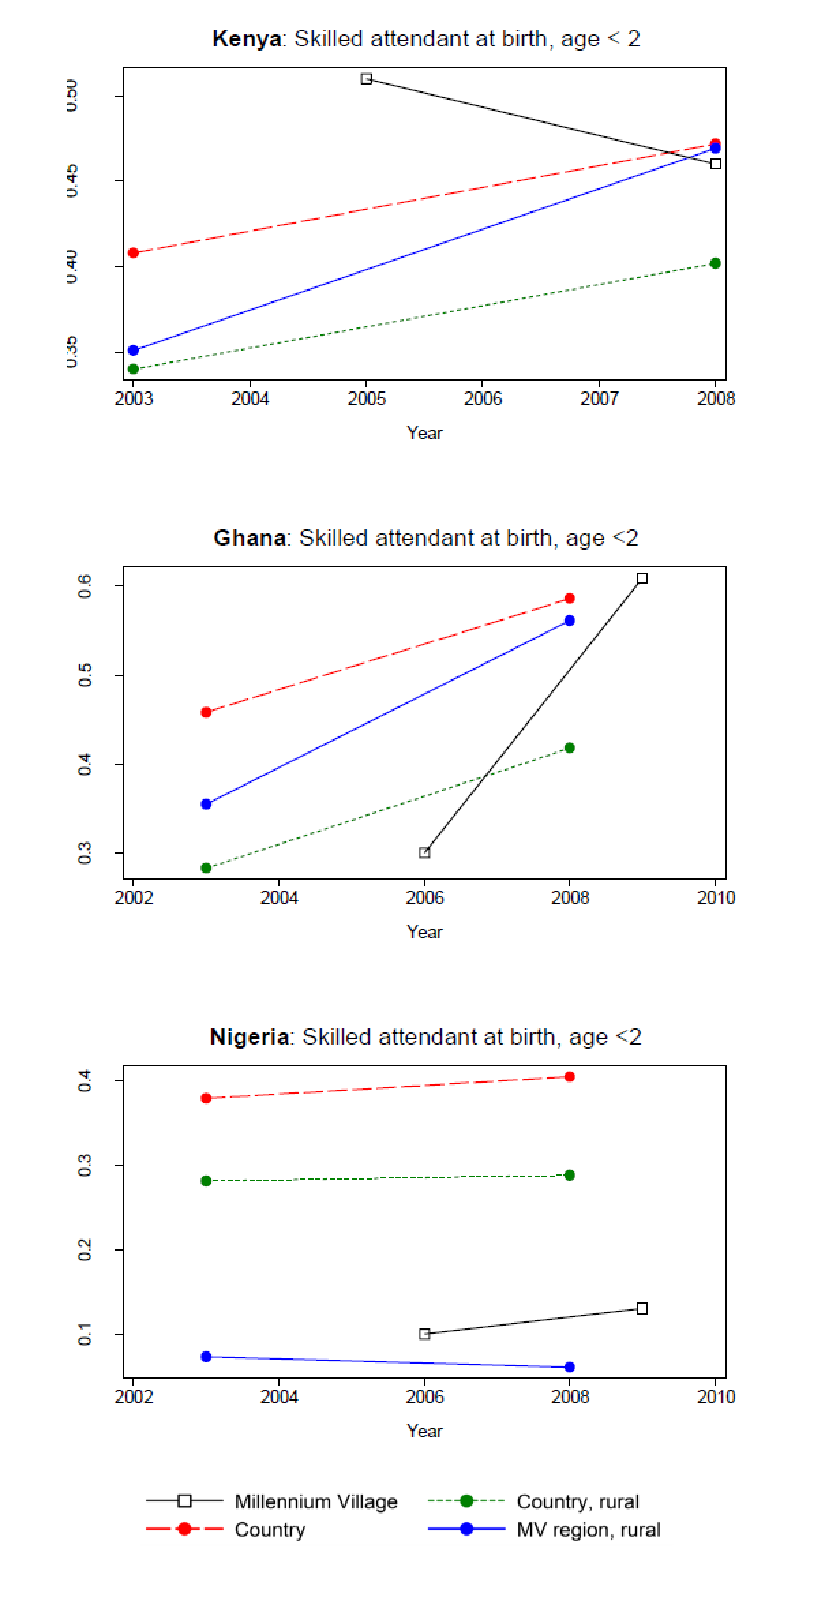
\includegraphics[keepaspectratio,height=5.0cm]{img/CD-skilled-births.pdf}}};
	\node [anchor=north east] (tab2) at (tab1.north west)  {\fbox{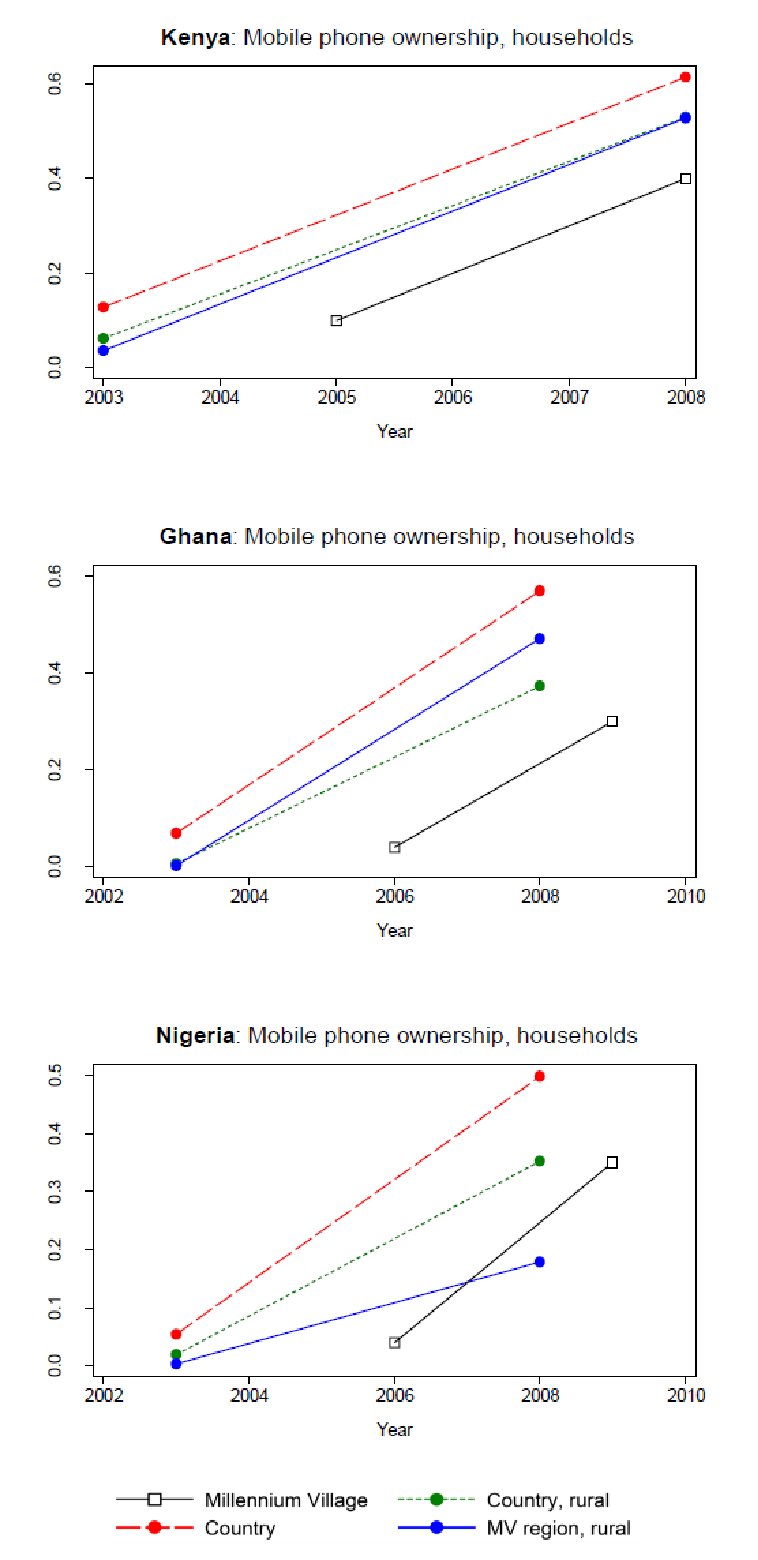
\includegraphics[keepaspectratio,height=5.0cm]{img/CD-phones.pdf}}};
	\node [anchor=north west] (tab3) at (tab1.north east)  {\fbox{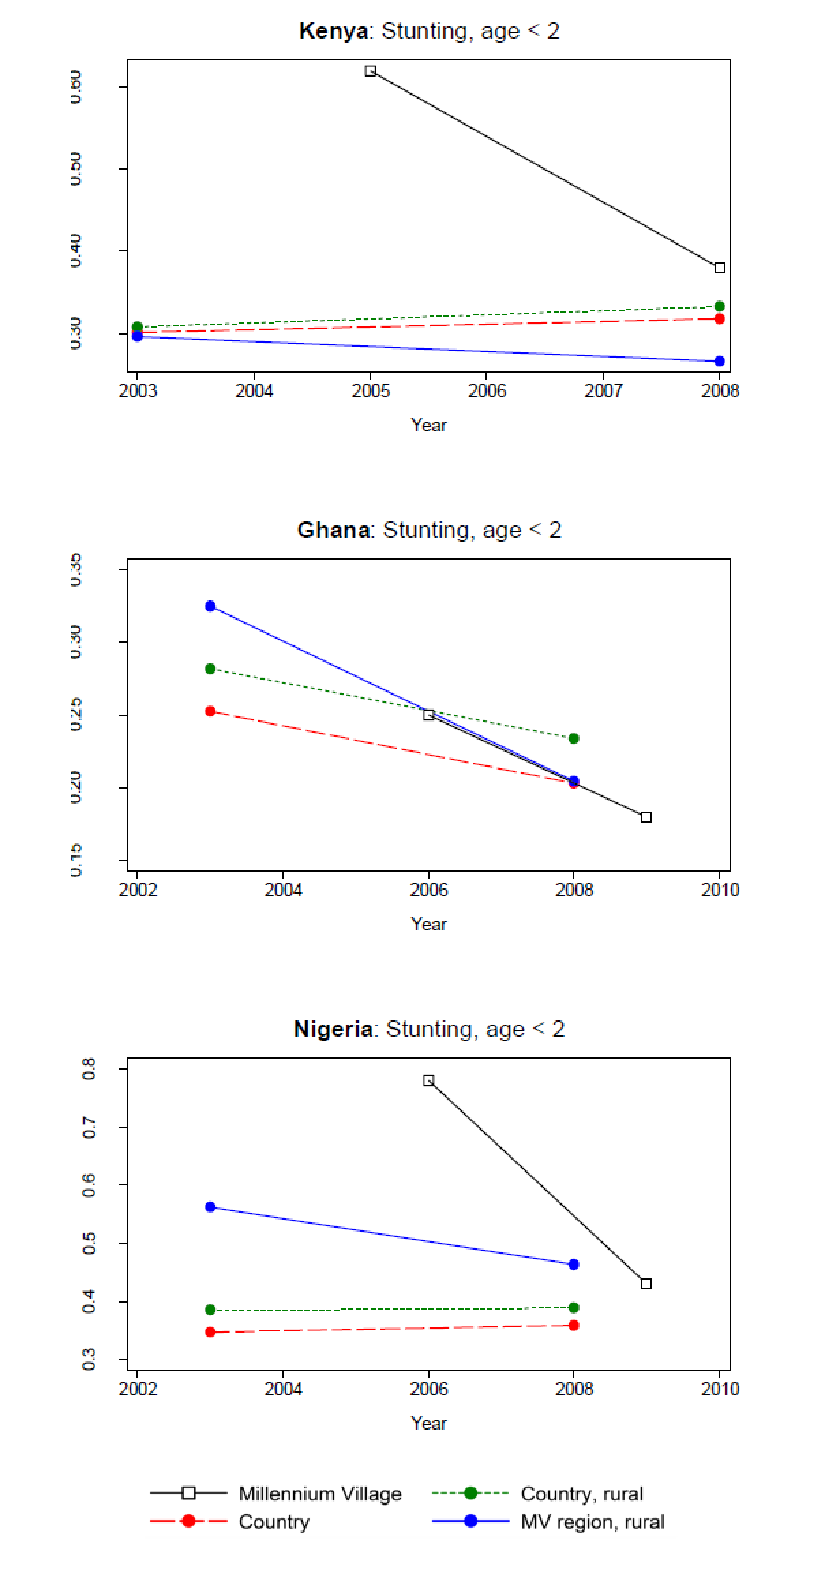
\includegraphics[keepaspectratio,height=5.0cm]{img/CD-stunting.pdf}}};
	
	\node [gray,anchor=north] at ([yshift=0.125cm]tab1.south)  {\tiny{source:  Clemens and Demombynes.~(2010)}};
	
	\end{tikzpicture}
\end{center}
\end{frame}



%%%%%%%%%%%%%%%%%%%%%%%%%%%%%%%%%%%%%%%%%%%%%%%%%%%%%%%%%%%%%%%%%%%%%%%

\begin{frame}{The Impacts of the Millennium Villages Project?}

\begin{center}
	\begin{tikzpicture}
	
	% blank canvas
	%\only<handout>{\fill[fill=white,draw=white,ultra thin]	(0,0) -- (11,0) -- (11,6) -- (0,6) -- cycle;}
	%\only<beamer>{\fill[fill=white,draw=white,ultra thin]	(0,0) -- (14,0) -- (14,6) -- (0,6) -- cycle;}
	\fill[fill=white,draw=white,ultra thin] (0,0) -- (14,0) -- (14,6) -- (0,6) -- cycle;
	%\only<beamer>{\draw[draw=oiblue!60,fill=oiblue!10,opacity=0.5] (11,1) rectangle (14,5);}
	%\draw[step=1.0,gray!20,thin] (0,0) grid (14,6);
	
	%	\pgfmathsetmacro\xshift{0.5cm};
	%	\pgfmathsetmacro\yshift{5.5cm};
	%	\pgfmathsetmacro\mycolor{"gray"};
	
	\node [anchor=north] (tab1) at (7,5.8)  {\fbox{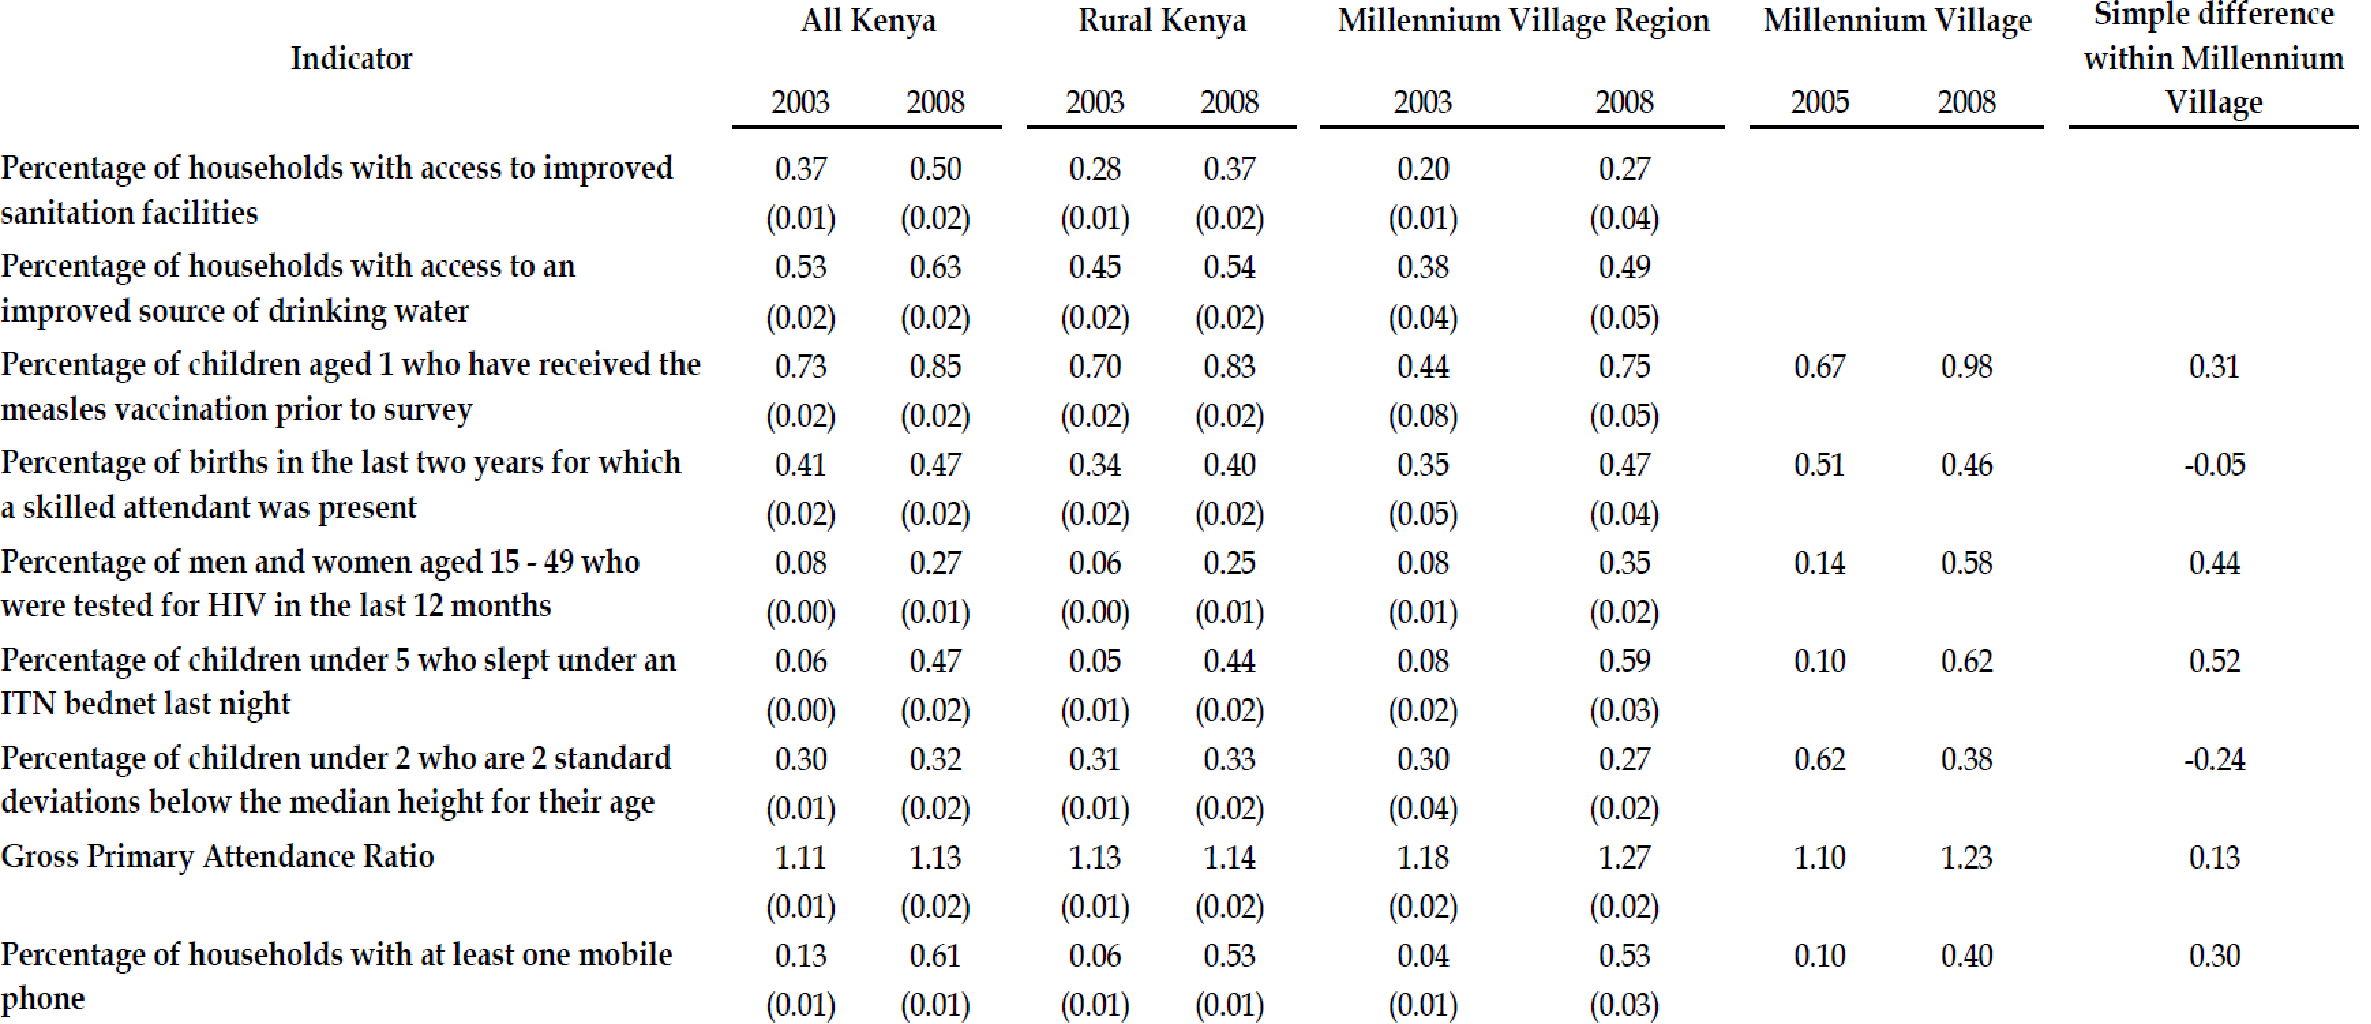
\includegraphics[keepaspectratio,height=4.8cm]{img/CD-means-no-DD.pdf}}};
	
	\node [gray,anchor=north] at ([yshift=0.125cm]tab1.south)  {\tiny{source:  Clemens and Demombynes.~(2010)}};
	
	\end{tikzpicture}
\end{center}
\end{frame}




%%%%%%%%%%%%%%%%%%%%%%%%%%%%%%%%%%%%%%%%%%%%%%%%%%%%%%%%%%%%%%%%%%%%%%%

\begin{frame}{The Impacts of the Millennium Villages Project?}

\begin{center}
	\begin{tikzpicture}
	
	% blank canvas
	%\only<handout>{\fill[fill=white,draw=white,ultra thin]	(0,0) -- (11,0) -- (11,6) -- (0,6) -- cycle;}
	%\only<beamer>{\fill[fill=white,draw=white,ultra thin]	(0,0) -- (14,0) -- (14,6) -- (0,6) -- cycle;}
	\fill[fill=white,draw=white,ultra thin] (0,0) -- (14,0) -- (14,6) -- (0,6) -- cycle;
	%\only<beamer>{\draw[draw=oiblue!60,fill=oiblue!10,opacity=0.5] (11,1) rectangle (14,5);}
	%\draw[step=1.0,gray!20,thin] (0,0) grid (14,6);
	
	%	\pgfmathsetmacro\xshift{0.5cm};
	%	\pgfmathsetmacro\yshift{5.5cm};
	%	\pgfmathsetmacro\mycolor{"gray"};
	
	\node [anchor=north] (tab1) at (7,5.8)  {\fbox{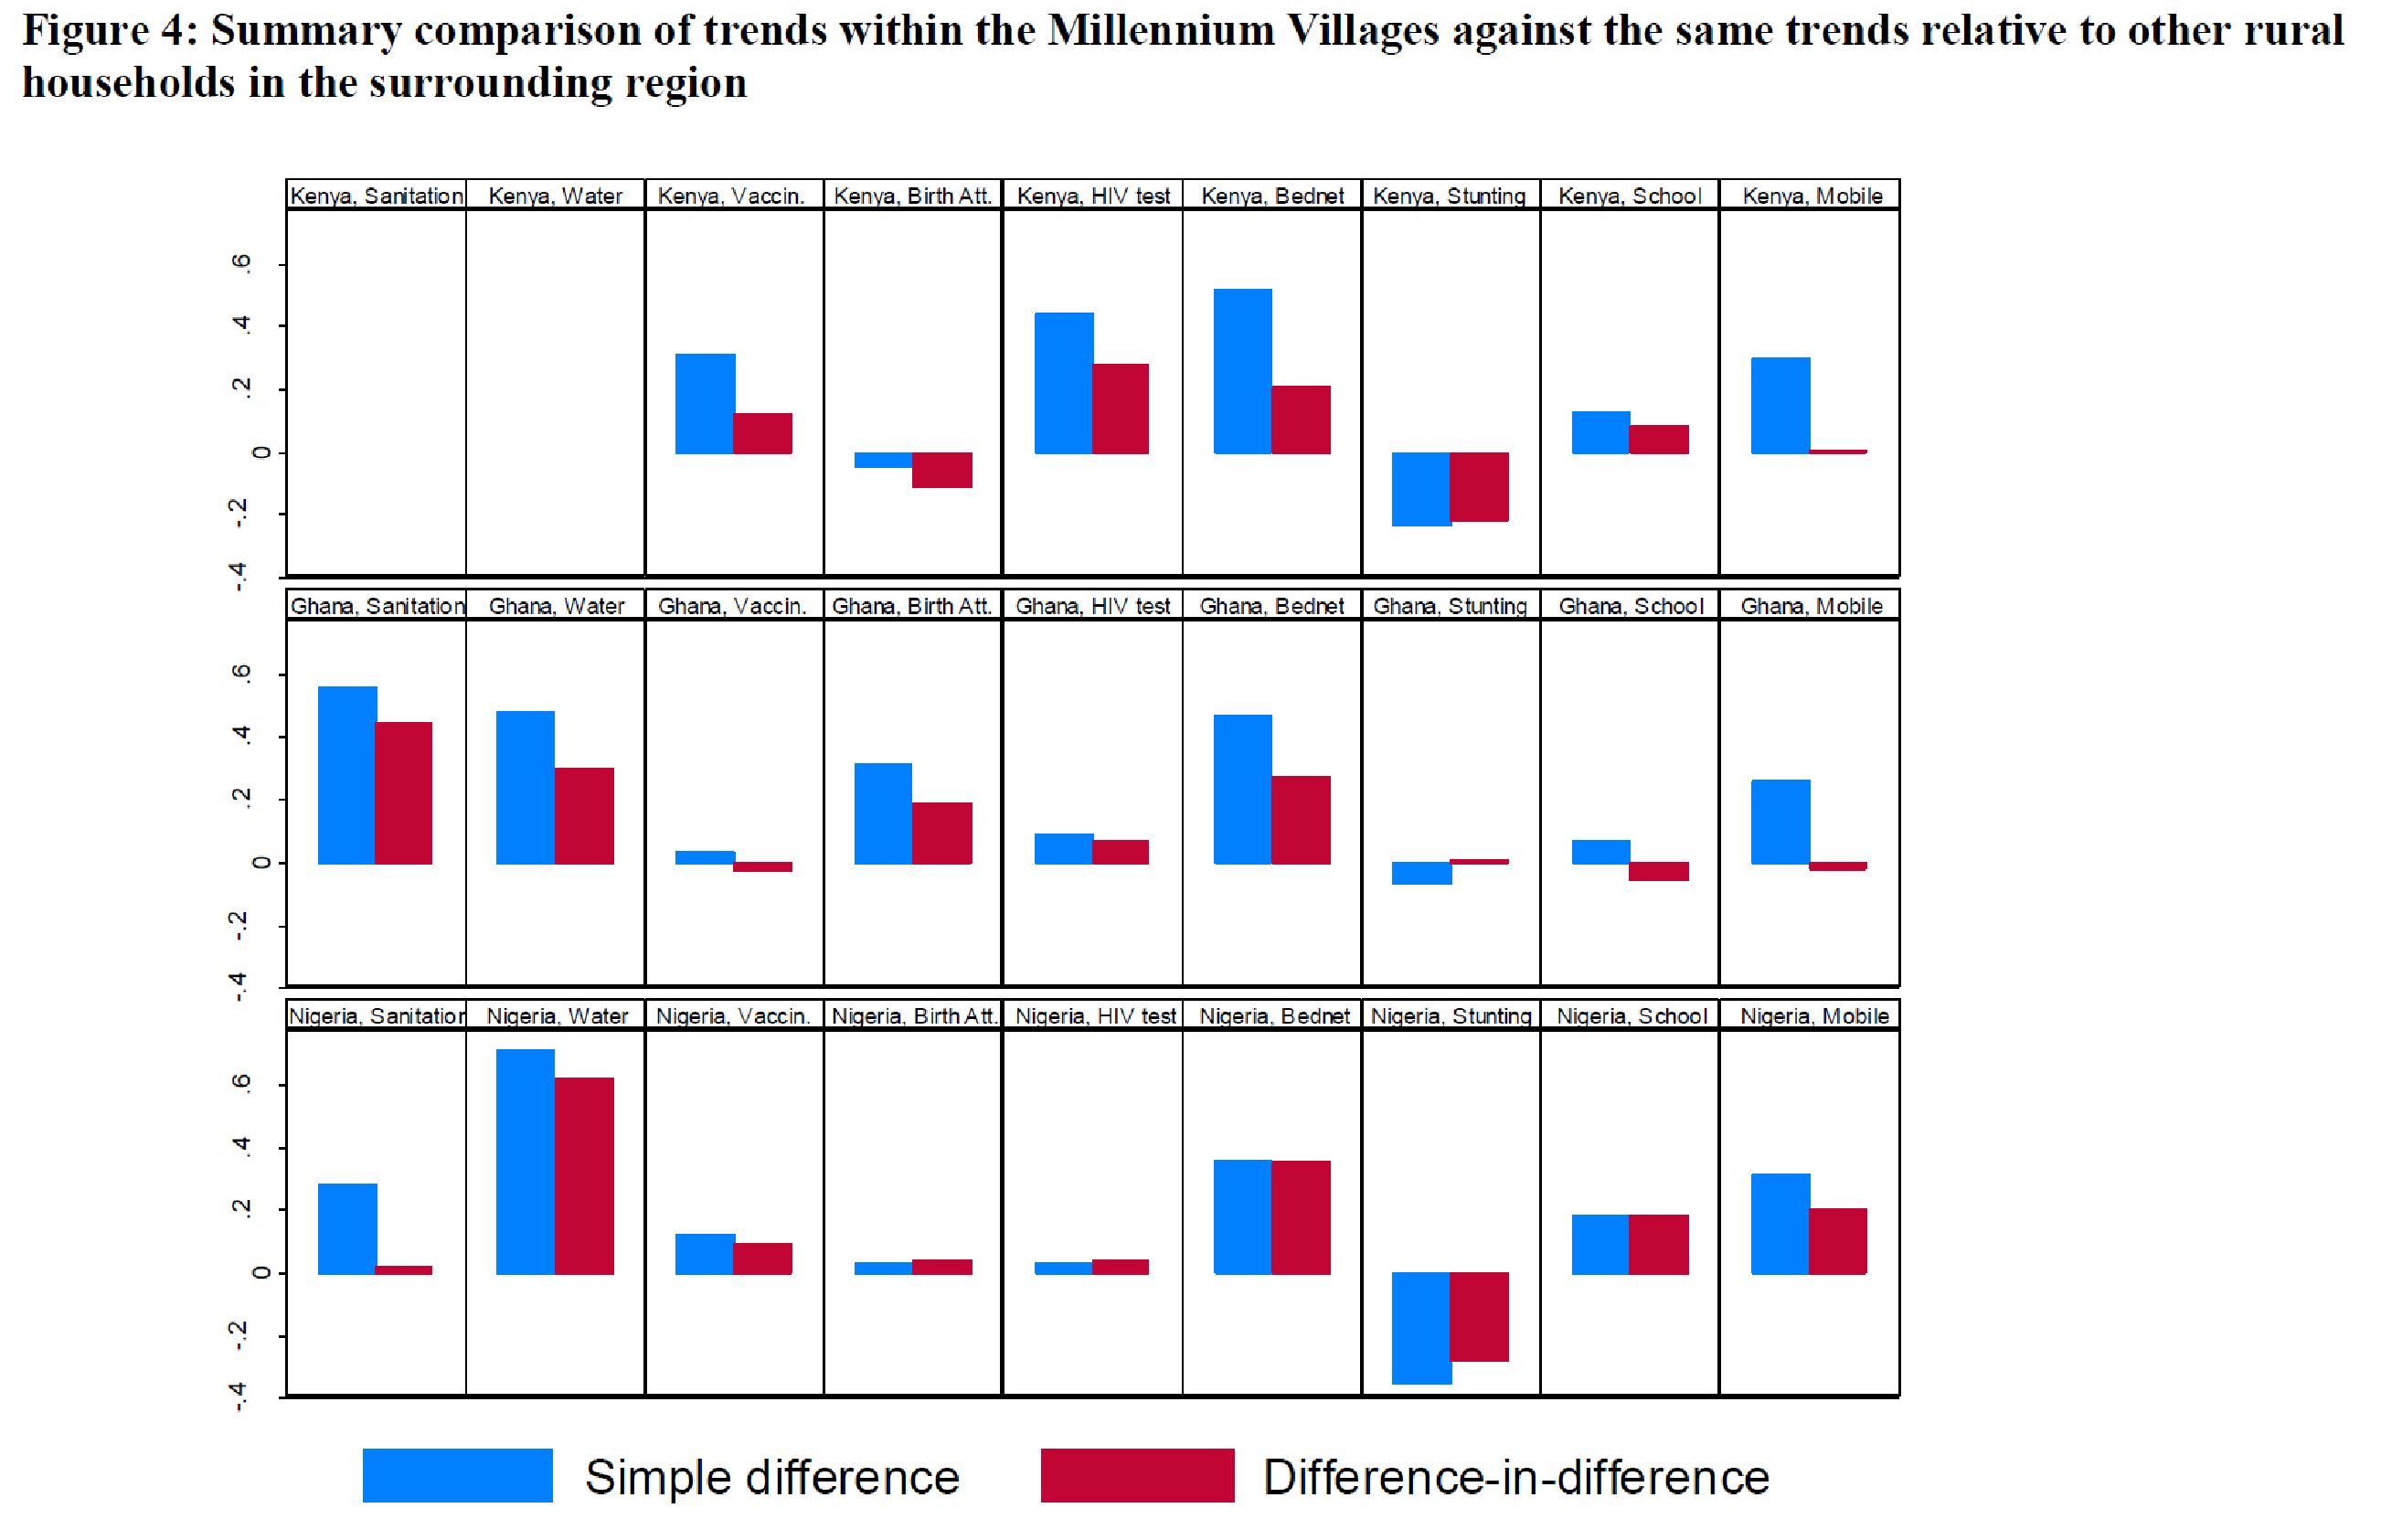
\includegraphics[keepaspectratio,height=4.8cm]{img/CD-DD-fig.pdf}}};
	
	\node [gray,anchor=north] at ([yshift=0.125cm]tab1.south)  {\tiny{source:  Clemens and Demombynes.~(2010)}};
	
	\end{tikzpicture}
\end{center}
\end{frame}




%%%%%%%%%%%%%%%%%%%%%%%%%%%%%%%%%%%%%%%%%%%%%%%%%%%%%%%%%%%%%%%%%%%%%%%%%%%

\begin{frame}[plain]

\only<beamer>{\begin{adjustwidth}{0cm}{-4cm}}

\begin{center}
	
	\Large{\textcolor{williams}{The end!}}
	
\end{center}

\only<beamer>{\end{adjustwidth}}
\end{frame}



\end{document}